\documentclass[11pt]{article}
\usepackage{amsmath, amssymb, amsfonts, mathtools}
%\usepackage{hyperref}
\usepackage[margin=1in]{geometry}
\usepackage{showlabels}
\usepackage{caption}
\newcommand{\tr}{\mathrm{tr}}
\newcommand{\ii}{\mathrm{i}}
\newcommand{\ep}{\epsilon}
\newcommand{\p}{\partial}
\newcommand{\dd}{\mathrm{d}}
\newcommand{\eps}{\varepsilon}
\newcommand{\mO}{\mathcal{O}}
\usepackage{
  jheppub
} % for details on the use of the package, please see the JINST-\
\newcommand{\nn}{\nonumber}
\usepackage{braket}
\newcommand{\lb}{\left(}
\newcommand{\rb}{\right)}
\usepackage{amsmath, amssymb}
\newcommand{\NL}[1]{\textcolor{blue}{#1}}
\usepackage{xcolor}

\newcommand{\JM}[1]{\textcolor{orange}{#1}}
\title{Relative entropy of mixtures of excited states in CFT}
\author{Nima Lashkari, Jignesh Mohanty to UIUC colleagues}
\affiliation{Department of Physics, Purdue University, West Lafayette, IN 47907, USA}
\emailAdd{nlashkari@purdue.edu}
%\abstract{We study the relative entropy of mixtures of excited states in conformal field theories in $1+1$ dimensions. We consider two energy eigenstates of a CFT $\ket{\mO_\alpha}$ and $\ket{\mO_\beta}$ corresponding to Virasoro primaries $\mO_{\alpha}$ and $\mO_{\beta}$. }


\begin{document}

\maketitle
\flushbottom
  \section{Introduction and Motivation}

  Consider a 2d CFT, and two energy eigenstates of $\ket{\mO_\alpha}$ and
  $\ket{\mO_\beta}$ corresponding to spinless Virasoro primaries $\Phi$ and
  $\Psi$. Denote by $\rho_\Phi$ and $\rho_\Psi$, the reduced density matrices of these states to a region $A$, and consider the mixture state $\rho_y=y\rho_\Phi+(1-y)\rho_\Psi$ for some $0\leq y\leq 1$. Motivated by connections to quantum error correction codes \cite{}, in this note, we study the relative entropies $S(\rho_\Phi\|\rho_y,A)$ in the small and large $|A|$ limits.
  
  
  % that for the mixture $(\rho_{\alpha}+\rho_{\beta})/2$ we
  % have the following asymptotic behavior of relative entropy
  % \begin{eqnarray}
  %   &&S(x):=S(\rho_\alpha|(\rho_\alpha+\rho_\beta)/2)\nn\\
  %   &&S(x)\simeq A_0 x^{\delta_0}, \qquad S(1-x)\simeq A_1(1-x)^{\delta_1},\nn\\
  %   &&\delta_1\leq \delta_0\ .
  % \end{eqnarray}
  % In this note, we check this conjecture. In particular, we will compute $\delta_1$ and $\delta_0$ in the special case of massless 2d free boson CFT and energy eigenstates created by the action of the vertex operator
  % states $V_{\alpha}=e^{i\alpha\phi}$ and $V_{\beta}= e^{i\beta\phi}$ at the
  % center of radial quantization. 

\section{Relative entropy of excited states}

\subsection{Setup and Replica Trick}

  Consider a conformal field theory (CFT) in $1+1$ dimensions on a cylinder
  $\mathcal{C}_{1}$ of circumference $R$. We focus on a spatial subsystem $A$ defined
  by the interval $(-l/2, l/2)$ at a fixed time slice. We simplify our notation
  by taking $A=(-\theta,\theta)$ on a cylinder of circumference $2\pi$ such that
  $\theta=\pi x$.

  Our states of interest are the reduced density matrices corresponding to
  energy eigenstates corresponding to the insertion of Virasoro primary fields at the center of radial quantization. These states are generated by the action of 
  % vertex operators $V_{\alpha}=:e^{i\alpha \phi}$
  % \JM{(
  operators $\Psi$ and $\Phi$ with conformal weights $(h_\Psi, \bar h_\Psi)$ and $(h_\Phi, \bar h_\Phi)$
  % )}: 
  % vertex operators $V_{\alpha}=:e^{i\alpha \phi}:$ 
  on the vacuum at past infinity in imaginary
  time on the Euclidean cylinder $\mathcal{C}_{1}$:
  % \begin{equation}
  %   |\alpha\rangle = \lim_{u\to i\infty}\frac{V_{\alpha}(u)|\Omega\rangle}{\braket{V_{-\alpha}(-u)V_\alpha(u)}^{1/2}}
  % \end{equation}
    \begin{equation}
    % \JM{
    |\Psi\rangle = \lim_{u\to i\infty}\frac{\Psi(u)|\Omega\rangle}{\braket{\Psi^*(-u)\Psi(u)}^{1/2}} \qquad |\Phi\rangle = \lim_{u\to i\infty}\frac{\Phi(u)|\Omega\rangle}{\braket{\Phi^*(-u)\Phi(u)}^{1/2}}
    % }
  \end{equation}
  % \JM{
  While considering the special case of massless free boson theory, we will replace these operators with Vertex operators.
  % }
  The reduced density matrix of the state   
  % $|\alpha\rangle$ 
  % \JM{(
  $|\Psi \rangle$
  % )}
  on the subsystem $A$
  is denoted by 
  % $\rho_{\alpha}$ \JM{(
  $\rho_\Psi$.
  % )}. 
  % A simple way to keep track of normalization of the
  % density matrix to define normalized operators
  % \begin{eqnarray}
  %   \tilde{V}_{\alpha}(u^+)\tilde{V}_{-\alpha}(u^-)=\frac{V_{\alpha}(u^{+})V_{-\alpha}(u^{-})}{\braket{V_{\alpha}(u^+)V_{-\alpha}(u^-)}_{\mathcal{C}_1}}
  % \end{eqnarray}
The replica trick that compute the relative entropy of excited states is
  % \begin{align}
  %   S\left(\rho_\alpha \Big\| \rho_\beta\right)&=\lb \partial_{n}
  %   \log \left[ \frac{\text{tr}(\rho_{\alpha}^{n})}{\text{tr}(\rho_{\alpha}\rho_{\beta}^{n-1})}
  %   \right]\rb_{n\to 1}\nn\\
  %   & =\lb\p_n\log\left[
  %   \frac{\braket{\prod_{i=1}^{n} V_{\alpha}(u^+_i)V_{-\alpha}(u^-_i)}_{\mathcal{C}_n}\braket{V_\beta(u^+)V_{-\beta}(u^-)}_{\mathcal{C}_1}^{n-1}}{\braket{V_\alpha(u^+_n)V_{-\alpha}(u^-_n)\mO^{(n-1)}_{\beta}}_{\mathcal{C}_n}\braket{V_\alpha(u^+)V_{-\alpha}(u^-)}_{\mathcal{C}_1}^{n-1}}\right]\rb_{n=1}\label{corrFncyl}\nn\\
  % \end{align}
  % where \JM{(this contains just the holomorphic part)}
  % \begin{eqnarray}
  %   &&\mO_{\beta}^{(n-1)}=
  %   V_{\beta}(u_1^+)V_{-\beta}(u_1^-)\cdots V_{\beta}(u_{n-1}^+)V_{-\beta}(u_{n-1}^-).
  % \end{eqnarray}
  \begin{align}\label{relEntropyReplica}
    S\left(\rho_\Psi \Big\| \rho_\Phi\right)&=\lb \partial_{n}
    \log \left[ \frac{\text{tr}(\rho_{\Psi}^{n})}{\text{tr}(\rho_{\Psi}\rho_{\Phi}^{n-1})}
    \right]\rb_{n\to 1}\nn\\
    % & =\lb\p_n\log\left[
    % \frac{\braket{\prod_{i=1}^{n} V_{\alpha}(u^+_{i,n}, \bar u_{i,n}^+)V_{-\alpha}(u^-_{i,n},\bar u_{i,n}^-)}_{\mathcal{C}_n}\braket{V_\beta(u^+,\bar u^+)V_{-\beta}(u^-,\bar u^-)}_{\mathcal{C}_1}^{n-1}}{\braket{V_\alpha(u^+_{n,n}, \bar u_{n,n}^+)V_{-\alpha}(u^-_{n,n},\bar u_{n,n}^-)\mO^{(n-1)}_{\beta}}_{\mathcal{C}_n}\braket{V_\alpha(u^+,\bar u^+)V_{-\alpha}(u^-,\bar u^-)}_{\mathcal{C}_1}^{n-1}}\right]\rb_{n=1}\label{corrFncyl}\nn\\
    % \JM{S(\rho_\Psi \| \rho_\Phi)}
    &=\lb
    % \JM{
    \p_n\log\left[
    \frac{\braket{\prod_{i=1}^{n} \Psi(u^+_{i,n}, \bar u_{i,n}^+)\Psi^*(u^-_{i,n},\bar u_{i,n}^-)}_{\mathcal{C}_n}\braket{\Phi(u^+,\bar u^+)\Phi^*(u^-,\bar u^-)}_{\mathcal{C}_1}^{n-1}}{\braket{\Psi(u^+_{n,n}, \bar u_{n,n}^+)\Psi^*(u^-_{n,n},\bar u_{n,n}^-)\mO^{(n-1)}_{\Phi}}_{\mathcal{C}_n}\braket{\Psi(u^+,\bar u^+)\Psi^*(u^-,\bar u^-)}_{\mathcal{C}_1}^{n-1}}\right]
    % }
    \rb_{n=1}
  \end{align}
  % \begin{eqnarray*}
  %   &&\mO_{\beta}^{(n-1)}=
  %   V_{\beta}(u_{1,n}^+,\bar u_{1,n}^+)V_{-\beta}(u_{1,n}^-, \bar u_{1,n}^-)\cdots V_{\beta}(u_{n-1,n}^+,\bar u_{n-1,n}^+)V_{-\beta}(u_{n-1,n}^-,\bar u_{n-1,n}^-).
  % \end{eqnarray*}
  \begin{eqnarray}\label{corrFncyl}
    % \JM{
    \mO_{\Phi}^{(n-1)}=
    \Phi(u_{1,n}^+,\bar u_{1,n}^+)\Phi^*(u_{1,n}^-, \bar u_{1,n}^-)\cdots \Phi(u_{n-1,n}^+,\bar u_{n-1,n}^+)\Phi^*(u_{n-1,n}^-,\bar u_{n-1,n}^-).
    % }
  \end{eqnarray}
   The conformal map \cite{Lashkari_2016}
  \begin{eqnarray}
    z=\lb\frac{\sin((u-\theta)/2)}{\sin((u+\theta)/2)}\rb^{1/n}
  \end{eqnarray}
  sends the interval $A=(-\theta,\theta)$ to $A=(0,\infty)$ uniformizing
  $\mathcal{C}_{n}$ to the complex plane. Under this transformation Virasoro primaries
  transform as
  \begin{eqnarray}
    &&\mO(u,\bar{u})=\lb\frac{\partial z}{\partial u} \rb^{h_\mO}\lb\frac{\partial
    \bar{z}}{\partial\bar{u}}
    \rb^{\bar{h}_\mO}\mO(z,\bar{z})\nn\\
    % &&V_\alpha(u_{k,n},\bar{u}_{k,n})=\lb\frac{z_{k,n}\Lambda}{n}\rb^{h_\alpha}\lb\frac{\bar{z}_{k,n}\Lambda}{n}\rb^{\bar{h}_\alpha}V_\alpha(z_{k,n},\bar{z}_{k,n}), \nn \\
    % &&\JM{
    &&\Psi(u_{k,n},\bar{u}_{k,n})=\lb\frac{z_{k,n}\Lambda}{n}\rb^{h_\alpha}\lb\frac{\bar{z}_{k,n}\Lambda}{n}\rb^{\bar{h}_\alpha}\Psi(z_{k,n},\bar{z}_{k,n}),
    % }
  \end{eqnarray}
  where in our example
  \begin{eqnarray}
    z_{k,n} = e^{\frac{2\pi ik}{n}},\qquad z^\pm_{k,n}=e^{\frac{i\pi}{n}(2k\pm x)},\qquad \Lambda=\frac{\sin(\theta)}{\cos(\theta)-\cos(u)}
  \end{eqnarray}
  We define 
%   \begin{align}
%   \mathcal{J}_{n,\alpha}&=\prod_{k=1}^{n-1}\lb \frac{\partial z^+_{k,n}}{\partial u^+_{k,n}}\rb^{h_\alpha}\lb \frac{\partial \bar{z}^+_{k,n}}{\partial \bar{u}^+_{k,n}}\rb^{\bar{h}_\alpha}\lb \frac{\partial z^-_{k,n}}{\partial u^-_{k,n}}\rb^{h_\alpha}\lb \frac{\partial \bar{z}^-_{k,n}}{\partial \bar{u}^-_{k,n}}\rb^{\bar{h}_\alpha}\nn\\
%   &=\prod_{k=1}^{n-1}\lb \frac{z^+_{k,n}z^-_{k,n}\Lambda^2}{n^2}\rb^{h_\alpha}\lb \frac{\bar{z}^+_{k,n}\bar{z}^-_{k,n}\Lambda^2}{n^2}\rb^{\bar{h}_\alpha}\nn\\
%   &=\prod_{k=1}^{n-1} (\Lambda/n)^{2(h_\alpha+\bar{h}_\alpha)}e^{4\pi i (h_\alpha-\bar{h}_\alpha)k/n}\nn\\
% %  &=n^{-2(n-1)(h_\alpha+\bar{h}_\alpha)}e^{2\pi i (n-1)(h_\alpha-\bar{h}_\alpha)}e^{-2\pi i (n-1)\bar{h}_\alpha}\nn\\
%   &=(\Lambda/n)^{2(n-1)\Delta_\alpha}e^{2\pi i(n-1) s_\alpha}
%   %=n^{-2(n-1)(\Delta_\alpha+\Delta_\beta)}
%   \end{align}
  \begin{align}
  \mathcal{J}_{n,\Psi}&=\prod_{k=1}^{n-1}\lb \frac{\partial z^+_{k,n}}{\partial u^+_{k,n}}\rb^{h_\Psi}\lb \frac{\partial \bar{z}^+_{k,n}}{\partial \bar{u}^+_{k,n}}\rb^{\bar{h}_\Psi}\lb \frac{\partial z^-_{k,n}}{\partial u^-_{k,n}}\rb^{h_\Psi}\lb \frac{\partial \bar{z}^-_{k,n}}{\partial \bar{u}^-_{k,n}}\rb^{\bar{h}_\Psi}\nn\\
  &=\prod_{k=1}^{n-1}\lb \frac{z^+_{k,n}z^-_{k,n}\Lambda^2}{n^2}\rb^{h_\Psi}\lb \frac{\bar{z}^+_{k,n}\bar{z}^-_{k,n}\Lambda^2}{n^2}\rb^{\bar{h}_\Psi}\nn\\
  &=\prod_{k=1}^{n-1} (\Lambda/n)^{2(h_\Psi+\bar{h}_\Psi)}e^{4\pi i (h_\Psi-\bar{h}_\Psi})k/n\nn\\
%  &=n^{-2(n-1)(h_\alpha+\bar{h}_\alpha)}e^{2\pi i (n-1)(h_\alpha-\bar{h}_\alpha)}e^{-2\pi i (n-1)\bar{h}_\alpha}\nn\\
  &=(\Lambda/n)^{2(n-1)\Delta_\Psi}e^{2\pi i(n-1) s_\Psi}
  %=n^{-2(n-1)(\Delta_\alpha+\Delta_\beta)}
  \end{align}
The overall conformal factor that captures the transformation of the correlator in (\ref{corrFncyl}) from the cylinder to the complex plane is
% \begin{align}
% \mathcal{J}&=\frac{\mathcal{J}_{n,\alpha}}{\mathcal{J}_{n,\beta}}\lb z^+_{1,1}z^-_{1,1}\Lambda^2\rb^{(n-1)(h_\beta-h_\alpha)}\lb\bar{z}^+_{1,1}\bar{z}^-_{1,1}\Lambda^2\rb^{(n-1)(\bar{h}_\beta-\bar{h}_\alpha)}\nn\\
% &=n^{-2(n-1)(\Delta_\alpha-\Delta_\beta)}e^{2\pi i(n-1)(s_\alpha-s_\beta)}
% \end{align}
\begin{align}
\mathcal{J}&=\frac{\mathcal{J}_{n,\Psi}}{\mathcal{J}_{n,\Phi}}\lb z^+_{1,1}z^-_{1,1}\Lambda^2\rb^{(n-1)(h_\Phi-h_\Psi)}\lb\bar{z}^+_{1,1}\bar{z}^-_{1,1}\Lambda^2\rb^{(n-1)(\bar{h}_\Phi-\bar{h}_\Psi)}\nn\\
&=n^{-2(n-1)(\Delta_\Psi-\Delta_\Phi)}e^{2\pi i(n-1)(s_\Psi-s_\Phi)}
\end{align}


 % where in the last step we have used the fact that $s_\alpha-s_\beta\in \mathbb{Z}$.
Therefore, mapping the correlator to the complex plane, we have 
% \begin{align}
%   S(\rho_\alpha\|\rho_\beta)=&\lb\p_n\log\mathcal{F}_n\rb_{n=1}\nn\\
%   \mathcal{F}_n&=\left[\frac{\braket{\prod_{i=1}^{n} V_{\alpha}(z^+_i)V_{-\alpha}(z^-_i)}\braket{V_\beta(z^+)V_{-\beta}(z^-)}^{n-1}}{\braket{V_\alpha(z^+_n)V_{-\alpha}(z^-_n)\tilde{\mO}^{(n-1)}_{\beta}}\braket{V_\alpha(z^+)V_{-\alpha}(z^-)}^{n-1}}\right]\lb \frac{e^{2\pi i (s_\alpha-s_\beta)}}{n^{2(\Delta_\alpha-\Delta_\beta)}}\rb^{n-1}\label{fncorrspin}\\
%   \tilde{\mO}^{(n-1)}_\beta&= \prod_{k=1}^{n-1} V_{\beta}(z^+_k)V_{-\beta}(z^-_k)
% \end{align}
\begin{align}
  S(\rho_\Psi\|\rho_\Phi)=&\lb\p_n\log\mathcal{F}_n\rb_{n=1}\nn\\
  \mathcal{F}_n&=\left[\frac{\braket{\prod_{i=1}^{n} \Psi (z^+_i)\Psi^(z^-_i)}\braket{\Phi(z^+)\Phi^*(z^-)}^{n-1}}{\braket{\Psi(z^+_n)\Psi^*(z^-_n)\tilde{\mO}^{(n-1)}_{\Phi}}\braket{\Psi(z^+)\Psi^*(z^-)}^{n-1}}\right]\lb \frac{e^{2\pi i (s_\Psi-s_\Phi)}}{n^{2(\Delta_\Psi-\Delta_\Phi)}}\rb^{n-1}\label{fncorrspin}\\
  \tilde{\mO}^{(n-1)}_\Phi&= \prod_{k=1}^{n-1} \Phi(z^+_k)\Phi^*(z^-_k)
\end{align}
% \NL{Add both $z$ and $\bar{z}$ dependence}
% \begin{align*}
%   S(\rho_\alpha\|\rho_\beta)=&\lb\p_n\log\mathcal{F}_n\rb_{n=1}\nn\\
%   \mathcal{F}_n&=\left[\frac{\braket{\prod_{i=1}^{n} V_{\alpha}(z^+_{i,n},\bar z^+_{i,n})V_{-\alpha}(z^-_{i,n},\bar z^-_{i,n})}\braket{V_\beta(z^+,\bar z^+)V_{-\beta}(z^-,\bar z^-)}^{n-1}}{\braket{V_\alpha(z^+_{n,n}, \bar z^+_{n,n})V_{-\alpha}(z^-_{n,n}, \bar z^-_{n,n})\tilde{\mO}^{(n-1)}_{\beta}}\braket{V_\alpha(z^+,\bar z^+)V_{-\alpha}(z^-,\bar z^-)}^{n-1}}\right]\lb \frac{e^{2\pi i (s_\alpha-s_\beta)}}{n^{2(\Delta_\alpha-\Delta_\beta)}}\rb^{n-1}\label{fncorrspin}\\
%   \tilde{\mO}^{(n-1)}_\beta&= \prod_{k=1}^{n-1} V_{\beta}(z^+_{k,n},\bar z^+_{k,n})V_{-\beta}(z^-_{k,n},\bar z^-_{k,n})
% \end{align*}
\begin{align}
  S(\rho_\Psi\|\rho_\Phi)=&\lb\p_n\log\mathcal{F}_n\rb_{n=1}\nn\\
  \mathcal{F}_n&=\left[\frac{\braket{\prod_{i=1}^{n} \Psi(z^+_{i,n},\bar z^+_{i,n})\Psi^*(z^-_{i,n},\bar z^-_{i,n})}\braket{\Phi(z^+,\bar z^+)\Phi^*(z^-,\bar z^-)}^{n-1}}{\braket{\Psi(z^+_{n,n}, \bar z^+_{n,n})\Psi^*(z^-_{n,n}, \bar z^-_{n,n})\tilde{\mO}^{(n-1)}_{\Phi}}\braket{\Psi(z^+,\bar z^+)\Psi^*(z^-,\bar z^-)}^{n-1}}\right]\lb \frac{e^{2\pi i (s_\Psi-s_\Phi)}}{n^{2(\Delta_\Psi-\Delta_\Phi)}}\rb^{n-1}\label{fncorrspin}\\
  \tilde{\mO}^{(n-1)}_\Phi&= \prod_{k=1}^{n-1} \Phi(z^+_{k,n},\bar z^+_{k,n})\Phi^*(z^-_{k,n},\bar z^-_{k,n})
\end{align}
Since $\Psi \Psi^*$ and $\Phi \Phi^*$ OPEs are invariant under a rotation of $\pi$ about its midpoint \cite{calabrese2011entanglement}, the total conformal spin should be an even integer. This requires $2s_\Psi, 2s_\Phi \in 2\mathbb{Z}$. Thus we have, $s_\Psi, s_\Phi \in \mathbb{Z}$ \cite{calabrese2011entanglement}. 
Since 
% $s_\alpha-s_\beta$ (\JM{
$s_\Psi-s_\Phi$
% })
is an integer, we drop the 
% $e^{2\pi i (s_\alpha-s_\beta)}$ (\JM{
$e^{2\pi i (s_\Psi-s_\Phi)}$ 
% }) 
term. \NL{Is this statement correct?}
% where we have used
% \begin{align}
%   \lb\p_n\log\left[n^{-2(n-1)(\Delta_\alpha+\Delta_\beta)}\right]\rb_{n\to 1}=0.
% \end{align}


% \NL{HERE}
%   Therefore, for normalized operators $\tilde{V}$ the contribution of $\Lambda$
%   terms cancel and we find\footnote{For scalar (spinless) operators in $2d$ we have $h_{\alpha}=\bar{h}_{\alpha}$
%   and we find
%   $\tilde{V}_{\alpha}(u_{k},\bar{u}_{k})=n^{-2h_\alpha}  \tilde{V}_{\alpha}(z_{k,n}
%     ,\bar{z}_{k,n})$.}
%   \begin{eqnarray}
%     \tilde{V}_\alpha(u^\pm_k,\bar{u}^\pm_k)&&=\lb\frac{z_{k,n}}{n z_{1,1}}\rb^{h_\alpha}\lb\frac{\bar{z}_{k,n}}{n
%     z_{1,1}}\rb^{\bar{h}_\alpha}\tilde{V}_\alpha(z_{k,n},\bar{z}_{k,n})\nn\\
%     &&=\lb\frac{e^{i\pi(2k\pm x)(1-n)/n}}{n }\rb^{h_\alpha}\lb\frac{e^{-i\pi(2k\pm
%     x)(1-n)/n}}{n}\rb^{\bar{h}_\alpha}\tilde{V}_\alpha(z^\pm_{k,n},\bar{z}^\pm_{k,n})
%   \end{eqnarray}
%   Therefore,
%   \begin{align}
%     \tilde{V}_\alpha(u^+_k,\bar{u}^+_k)\tilde{V}_{\alpha}(u^-_k,\bar{u}^-_k)=n^{-2\Delta_\alpha}e^{4\pi i k s_\alpha(n-1)/n}\tilde{V}_\alpha(z^+_{k,n},\bar{z}^+_{k,n})\tilde{V}_\alpha(z^-_{k,n},\bar{z}^-_{k,n})
%   \end{align}
% The relative entropy replica trick in terms of the correlator on the complex plane gives
%   \begin{align}\label{CorrFn}
%     S(\rho_\alpha\|\rho_\beta)&=\lb \partial_n\log\mathcal{F}_n(\alpha|\beta)\rb_{n\to 1}\nn\\
%     \mathcal{F}_n(\alpha|\beta)&=
%     \frac{\braket{\prod_{k=1}^{n} \tilde{V}_{\alpha}(z^+_{k,n})\tilde{V}_{-\alpha}(z^-_{k,n})}}{\braket{\tilde{V}_\alpha(z^+_{n,n})\tilde{V}_{-\alpha}(z^-_{n,n})\tilde{\mO}^{(n-1)}_{\beta}}}\nn\\
%     \tilde{\mO}_{\beta}^{(n-1)}&=n^{2(n-1)(\Delta_\alpha-\Delta_\beta)}\prod_{k=1}^{n-1}\lb e^{4\pi i k (s_\beta-s_\alpha)(n-1)/n}\frac{V_{\beta}(z_{k,n}^{+})V_{-\beta}(z_{k,n}^{-})}{\braket{V_{\beta}(z^+_{1,1})V_{-\beta}(z^-_{1,1})}}\rb\nn\\
%     &=n^{2(n-1)(\Delta_\alpha-\Delta_\beta)}e^{2\pi i (s_\beta-s_\alpha)(n-1)^2}\prod_{k=1}^{n-1}\frac{V_{\beta}(z_{k,n}^{+})V_{-\beta}(z_{k,n}^{-})}{\braket{V_{\beta}(z^+_{1,1})V_{-\beta}(z^-_{1,1})}}.
%   \end{align}
%   Note that the term $e^{2\pi i (s_\alpha-s_\beta)(n-1)^2}$ term does not contribute to relative entropy because
%   \begin{align}
%       &-\p_n\lb 2\pi i (s_\alpha-s_\beta)(n-1)^2\rb_{n\to 1}=0
%   \end{align}
%   As a result, we can drop this term from the denominator. 
 % We will specialize to the case where $s_\alpha=s_\beta$ so that we can drop the contribution of the spin.

  % \subsection{Small interval limit $x\to 0^+$}
\subsection{Small interval limit \texorpdfstring{$x\to 0^+$}{x -> 0+}}
Label by $\mO_L$, $\mO_{L''}$, and $\mO_{L'}$ the lightest Virasoro primaries that appear, respectively, in the OPE of $\Psi \Psi^*$, $\Phi\Phi^*$, and $\Psi\Phi^*$\footnote{Otherwise the lowest order
  term would come from stress tensor.}. 
  To simplify our notation, we define
   % \JM{(
   $C_{\Psi} = C^{L}_{\Psi\Psi^*}$, $C_{\Phi} = C^{L''}_{\Phi\Phi^*}$ and $C_{\Psi \Phi} = C^{L'}_{\Psi \Phi^*}=C^{L'}_{\Psi^*\Phi}$\footnote{Note that $C^{L'}_{\Psi\Phi^*}=(C^{L'}_{\Psi^*\Phi})^*$, but in a unitary CFT, the OPE coefficients are real.}.
   % )
   % } 
   % $C_{\omega}=C^{L}_{\omega(-\omega)}$ for $\omega=\alpha,\beta$ and $C_{\alpha\beta}=C^L_{\alpha\beta}$ 
   In the small $x$ limit, we can expand in the OPE
  channel
  % \begin{align}
  %   \frac{V_{w_k}(z_{k}^{+})V_{-w_k}(z_{k}^{-})}{\braket{V_{w_k}(z^+)V_{-w_k}(z^-)}}&=e^{-4\pi i k s_{w_k}/n}\lb
  %   \frac{\sin(\pi x)}{\sin(\pi x/n)}\rb^{2\Delta_{w_k}}\times\nn\\
  %   &\quad\lb 1+ C_{w_k}(2\sin(\pi x/n))^{\Delta_L}e^{\pi i s_L(2k/n+1/2)}\mO_L(e^{2\pi i k/n})+\cdots\rb
  % \end{align}
  \begin{align}
    \frac{\Psi(z_{k}^{+})\Psi^*(z_{k}^{-})}{\braket{\Psi(z^+)\Psi^*(z^-)}}&=e^{-4\pi i k s_{\Psi}/n}\lb
    \frac{\sin(\pi x)}{\sin(\pi x/n)}\rb^{2\Delta_{\Psi}}\times\nn \\
    &\quad\lb  1+ C_{\Psi}(2\sin(\pi x/n))^{\Delta_L}e^{\pi i s_L(2k/n+1/2)}\mO_L(e^{2\pi i k/n})+\rb  \\
    \frac{\Phi(z_{k}^{+})\Phi^*(z_{k}^{-})}{\braket{\Phi(z^+)\Phi^*(z^-)}}&=e^{-4\pi i k s_{\Phi}/n}\lb
    \frac{\sin(\pi x)}{\sin(\pi x/n)}\rb^{2\Delta_{\Phi}}\times\nn\\
    &\quad\lb  1+ C_{\Phi}(2\sin(\pi x/n))^{\Delta_{L''}}e^{\pi i s_{L''}(2k/n+1/2)}\mO_{L''}(e^{2\pi i k/n})+\cdots\rb 
  \end{align}
  % \begin{align*}
  %   \JM{\frac{V_{w_k}(z_{k,n}^{+},\bar z_{k,n}^+)V_{-w_k}(z_{k,n}^{-},\bar z_{k,n}^-)}{\braket{V_{w_k}(z^+)V_{-w_k}(z^-)}}}&=e^{-4\pi i k s_{w_k}/n}\lb
  %   \frac{\sin(\pi x)}{\sin(\pi x/n)}\rb^{2\Delta_{w_k}}\times\nn\\
  %   &\quad\lb 1+ C_{w_k}(2\sin(\pi x/n))^{\Delta_L}e^{\pi i s_L(2k/n+1/2)}\mO_L(e^{2\pi i k/n})+\cdots\rb
  % \end{align*}
  In our notation, the Virasoro primary $\mO_{L}$ has
  dimensions $(h_{L},\bar{h}_{L})$, weight $\Delta_{L}=h_{L}+\bar{h}_{L}<2$ and spin $s_{L}=h_{L}-\bar{h}_{L}$. Depending on the theory, there might be several operators contributing at the lowest order. In this case, we will have to sum over all possible operators.
We simplify our notation by keeping the sum over all possible operators implicit. Note that the factors coming from spins of $V_\alpha$ and $V_\beta$ becomes
% \begin{align}
%  \prod_{k=1}^{n-1} e^{-4\pi i k (s_\alpha-s_\beta)/n}=e^{-2\pi i (n-1)(s_\alpha-s_\beta)}
% \end{align}
\begin{align}
 \prod_{k=1}^{n-1} e^{-4\pi i k (s_\Psi-s_\Phi)/n}=e^{-2\pi i (n-1)(s_\Psi-s_\Phi)}
\end{align}
which precisely cancels out the that of equation (\ref{fncorrspin}).
Therefore, the analytic correlator we need to compute to find the relative entropy is
  \begin{align}
    \label{eq:F_n}\mathcal{F}_{n} & =\frac{\lb\,1+(2\sin(\pi x/n))^{2\Delta_L}f(n)+\cdots\,\rb}{\lb D_n(x)^{n-1}\left[\,1+(2\sin(\pi x/n))^{2\Delta_L}g(n)+\cdots\,\right] \rb}\\
    \label{Dn}
    D_{n}(x)&=\left(\frac{n\sin(\pi x/n)}{\sin(\pi x)}\right)^{2(\Delta_\Psi-\Delta_\Phi)}
    ,\qquad D_{1}(x)=1,
  \end{align}
  where the leading correction $f(n)$ and $g(n)$ are given by the sums in (\ref{fnexpression1}) and (\ref{gnw1}), respectively, over OPE coefficients and light operator correlators on the replica manifold. 
  First, observe that $D_n(x)^{n-1}$ term does not contribute to relative entropy:
  \begin{align}
  &-\p_n\lb (n-1)\log D_n(x)\rb_{n\to 1}=0,
  \end{align}
Hence, we drop it from the denominator, and
  \begin{align}
    % S(\rho_\alpha\|\rho_\beta)\to
    S(\rho_\Psi  \| \rho_\Phi)&=\p_n\left[\log \frac{1+\xi^{2\Delta_L} f(n)+\cdots}{1+\xi^{2\Delta_L} g(n)+\cdots}\right]_{n=1}=\xi^{2\Delta_L}\p_n\left[f(n)-g(n)\right]_{n=1}+\cdots\nn\\
    \xi&=\frac{2\pi x}{n}\ll 1.
  \end{align}
where
  % \begin{align}\label{fnexpression1}
  %   f(n) & =e^{i\pi s_L} \frac{C_{\alpha}^{2}}{2}\sum_{k\neq k'=0}^{n-1}e^{2\pi i s_L (k+k')/n}\langle \mO_{L}(e^{2\pi i k/n})\mO_{L}(e^{2\pi i k'/n})\rangle \nn    \\
  %   &=\frac{e^{i\pi s_L} C_\alpha^2}{2}\sum_{k\neq k'=0}^{n-1}(2i\sin(\pi(k-k')/n))^{-2h_L}(-2i\sin(\pi(k-k')/n))^{-2\bar{h}_L}\nn\\
  %        & =\frac{C_{\alpha}^{2}}{2}\sum_{k\neq k'=0}^{n-1}\frac{1}{(2\sin(\pi |k-k'|/n))^{2\Delta_L}}\ .
  % \end{align}
  \begin{align}\label{fnexpression1}
    f(n) & =e^{i\pi s_L} \frac{C_{\Psi}^{2}}{2}\sum_{k\neq k'=0}^{n-1}e^{2\pi i s_L (k+k')/n}\langle \mO_{L}(e^{2\pi i k/n})\mO_{L}(e^{2\pi i k'/n})\rangle \nn    \\
    &=\frac{e^{i\pi s_L} C_{\Psi}^2}{2}\sum_{k\neq k'=0}^{n-1}e^{-i\pi s_L}(2i\sin(\pi(k-k')/n))^{-2h_L}(-2i\sin(\pi(k-k')/n))^{-2\bar{h}_L}\nn\\
         & =\frac{C_{\Psi}^2}{2}\sum_{k\neq k'=0}^{n-1}\frac{1}{(2\sin(\pi |k-k'|/n))^{2\Delta_L}}\ .
  \end{align}
  % Rewrite the sum above by fixing the separation $m:=k-k' \ (\mathrm{mod}\ n)$. For
  % each $m\in\{1,2,\dots,n-1\}$, set $k'=k-m$ (mod $n$). Then
  % \[
  %   e^{-2\pi i s_L (k+k')/n}= e^{-2\pi i s_L (2k-m)/n}= e^{+2\pi i s_L m/n}\,e^{-4\pi
  %   i s_L k/n},
  % \]
  % and the denominator depends only on $m$. Hence the sum factorizes:
  % \begin{equation}
  %   \sum_{m=1}^{n-1}\frac{e^{2\pi i s_L m/n}}{\bigl(2\sin\frac{\pi m}{n}\bigr)^{2\Delta_L}}
  %   \underbrace{\sum_{k=0}^{n-1} e^{-4\pi i s_L k/n}}_{=:G(n)}.
  % \end{equation}
  % The inner sum $G(n)$ is a geometric series with ratio $q=e^{-4\pi i s_L/n}$:
  % \[
  %   G(n)=\sum_{k=0}^{n-1}q^{k}=
  %   \begin{cases}
  %     n, & q=1,     \\
  %     0, & q\neq 1.
  %   \end{cases}
  % \]
  % Therefore $S(n)=0$ for integer $n$ unless $q=1$, i.e.
  % \[
  %   e^{-4\pi i s_L/n}=1 \quad\Longleftrightarrow\quad \frac{4s_{L}}{n}\in\mathbb{Z}
  %   .
  % \]
  % Now, since $4s_{L}/n$ is not an integer, the numerator $e^{2\pi i s_L m/n}$ is
  % at most a sign. For $s_L=0$, we are left with
  The analytic continuation
  \begin{align}
     & S_{2}(n,\Delta_L)=\frac{n}{2}\sum_{k=1}^{n-1}(2\sin(\pi k/n))^{-2\Delta_L},\qquad S_{2}(1,\Delta_L)=0,
  \end{align}
  was discussed in
  \cite{calabrese2011entanglement}\footnote{Note that our notation has an extra factor $2^{-2\Delta_L}$.}
  \begin{align}
    S'_{2}(1,\Delta)=\frac{2^{-2\Delta}\sqrt{\pi}\Gamma(\Delta+1)}{4\Gamma(\Delta+3/2)}\ .
  \end{align}
  Therefore,
  \begin{align}
    f'(1)=C^2_\Psi \frac{2^{-2\Delta}\sqrt{\pi}\Gamma(\Delta+1)}{4\Gamma(\Delta+3/2)}
  \end{align}
  In a general CFT, there could be several inequivalent choices of the lightest primary
  operator $\mO_{L}$ that contribute at the same order. In this case, the leading
  correction $f(n)$ would be given by the sum over all such operators, that
  following \cite{calabrese2011entanglement} we denote by
  \begin{align}
    f(n) & = C_\Psi^2 S_{2}(n,\Delta) 
  \end{align}
  % \begin{align*}
  %     \JM{f(n) = C_\alpha^2 S_2(n)}
  % \end{align*}
The denominator in $\mathcal{F}_n$ depends on how $\Delta_L$ and $\Delta_{L''}$ compare. We first consider the case, $\Delta_L=\Delta_{L''}$. Then,
  % \begin{align}\label{gnw1}
  %   g(n)= & C_{\alpha}C_\beta\sum_{k=1}^{n-1}\frac{1}{(2\sin(\pi k/n))^{2\Delta_L}}+\frac{C_\beta^2}{2}\sum_{k\neq k'=1}^{n-1}\frac{1}{(2\sin(\pi |k-k'|/n))^{2\Delta_L}}, \nn\\% \nn\\
  %   =&(C_\alpha-C_\beta)C_\beta\sum_{k=1}^{n-1}\frac{1}{(2\sin(\pi k/n))^{2\Delta_L}}+C_\beta^2 S_2(n)
  %   % &=C_\alpha C_\omega \frac{2 S_2(n)}{n}+\sum_{k\neq k'=1}^{n-1}
  %   % \frac{C_{w_k}C_{w_{k'}}}{(2\sin(\pi |k-k'|/n))^{4h_L}}
  % \end{align}
  \begin{align}\label{gnw1}
    g(n)= & C_{\Psi}C_\Phi\sum_{k=1}^{n-1}\frac{1}{(2\sin(\pi k/n))^{2\Delta_L}}+\frac{C_\Phi^2}{2}\sum_{k\neq k'=1}^{n-1}\frac{1}{(2\sin(\pi |k-k'|/n))^{2\Delta_{L}}}, \nn\\% \nn\\
    =&(C_\Psi -C_\Phi)C_\Phi\sum_{k=1}^{n-1}\frac{1}{(2\sin(\pi k/n))^{2\Delta_L}}+C_\Phi^2 S_2(n,\Delta_{L})
    % &=C_\alpha C_\omega \frac{2 S_2(n)}{n}+\sum_{k\neq k'=1}^{n-1}
    % \frac{C_{w_k}C_{w_{k'}}}{(2\sin(\pi |k-k'|/n))^{4h_L}}
  \end{align}
Therefore, expanding in small $x$ we find
% \begin{align}
%   &\log\mathcal{F}_n(x)=(2\pi x/n)^{2\Delta_L}\lb(C_\alpha^2-C_\beta^2)S_2(n)-(C_\alpha-C_\beta)C_\beta \frac{2S_2(n)}{n}\rb+\cdot
% \end{align}
\begin{align}
  &\log\mathcal{F}_n(x)=(2\pi x/n)^{2\Delta_L}\lb(C_\Psi^2-C_\Phi^2)S_2(n)-(C_\Psi-C_\Phi)C_\Phi \frac{2S_2(n,\Delta_L)}{n}\rb+\cdot
\end{align}
Since $S_2(1,\Delta)=0$ we find
% \begin{align}
% S(\rho_\alpha\|\rho_\beta)=&(C_\alpha-C_\beta)^2 S'_2(1)(2\pi x)^{2\Delta_L}+\cdots \nn\\
% &=(C_\alpha-C_\beta)^2 \frac{\sqrt{\pi}\Gamma(\Delta_{L}+1)}{4\Gamma(\Delta_{L}+3/2)}(\pi x)^{2\Delta_L}+\cdots
% \end{align}
\begin{align}
% \JM{
S(\rho_\Psi\|\rho_\Phi)
% }
=&
% \JM{
(C_\Psi-C_\Phi)^2 S'_2(1,\Delta_L)(2\pi x)^{2\Delta_L}+\cdots \nn\\
&=(C_\Psi-C_\Phi)^2\frac{\sqrt{\pi}\Gamma(\Delta_{L}+1)}{4\Gamma(\Delta_{L}+3/2)}(\pi x)^{2\Delta_L}+\cdots
\end{align}

Next, consider the case $\Delta_{L''}<\Delta_L$. In this case, only the denominator of $\mathcal{F}_n$ contributes to the lowest order, and we have
  \begin{align}\label{gnw1p}
    g(n)= & \frac{C_\Phi^2}{2}\sum_{k\neq k'=1}^{n-1}\frac{1}{(2\sin(\pi |k-k'|/n))^{2\Delta_{L''}}}, \nn\\% \nn\\
    =&-C_\Phi^2\sum_{k=1}^{n-1}\frac{1}{(2\sin(\pi k/n))^{2\Delta_{L''}}}+C_\Phi^2 S_2(n,\Delta_{L''})
    % &=C_\alpha C_\omega \frac{2 S_2(n)}{n}+\sum_{k\neq k'=1}^{n-1}
    % \frac{C_{w_k}C_{w_{k'}}}{(2\sin(\pi |k-k'|/n))^{4h_L}}
  \end{align}
and since we assumed $\Delta_{L''}$
\begin{align}
  \log\mathcal{F}_n(x)&=(2\pi x/n)^{2\Delta_{L''}}\lb -C_\Phi^2 S_2(n,\Delta_{L''})+C_\Phi^2 \frac{2S_2(n,\Delta_{L''})}{n}\rb+\cdot\nn\\
% \JM{
S(\rho_\Psi\|\rho_\Phi)
% }
=&
% \JM{
C_\Phi^2 S'_2(1,\Delta_{L''})(2\pi x)^{2\Delta_{L''}}+\cdots \nn\\
&=C_\Phi^2\frac{\sqrt{\pi}\Gamma(\Delta_{L''}+1)}{4\Gamma(\Delta_{L''}+3/2)}(\pi x)^{2\Delta_{L''}}+\cdots
\end{align}

Finally, consider the case $\Delta_{L''}>\Delta_L$, then only the numerator contributes to the lowest order to $\mathcal{F}_n$, and we have
\begin{align}
% \JM{
S(\rho_\Psi\|\rho_\Phi)
% }
=&
% \JM{
C_\Psi^2 S'_2(1,\Delta_{L})(2\pi x)^{2\Delta_{L}}+\cdots \nn\\
&=C_\Psi^2\frac{\sqrt{\pi}\Gamma(\Delta_{L}+1)}{4\Gamma(\Delta_{L}+3/2)}(\pi x)^{2\Delta_{L}}+\cdots
\end{align}
The lesson to learn here is that when $\Delta_{L''}<\Delta_{L}$, to the lowest order the calculation is the same as $S(\rho_0\|\rho_\Phi)$, and when $\Delta_{L''}>\Delta_L$, to the lowest order, it is the same as $S(\rho_\Psi\|\rho_0)$, with $\rho_0$ the vacuum reduced state. As a result, in the remainder of this draft, with no loss of generality, we focus on the case $\Delta_L=\Delta_{L''}$ to simplify our notation. 

Stress tensors $T$ and $\bar{T}$ contribute to the OPE expansion with weights $(2,0)$ and $(0,2)$. In theories with conserved currents $J$ and $\bar{J}$ (e.g. Kac-Moody algebras), these currents have weights $(1,0)$ and $(0,1)$. Therefore, to the lowest order in small $x$ expansion, in any 2d CFT with a relevant deformation $\Delta_L<1$, we can ignore these corrections. 

 % \subsection{Relative entropy $S(\rho_\alpha\|\rho_\beta)$ in the limit $x\to 0^+$}

  In the small interval limit, $x\to 0^+$, the relative entropy of primary states of dimension 
  % $(h_\alpha,\bar{h}_\alpha)$ and $(h_\beta,\bar{h}_\beta)$
  $(h_\Psi,\bar{h}_\Psi)$ and $(h_\Phi,\bar{h}_\Phi)$
  is universal and given by \ref{Ssmallx}
  % \begin{align}
  % S(\rho_\alpha\|\rho_\beta)=\begin{cases}
  % \frac{\sqrt{\pi}\Gamma(\Delta+1)}{4\Gamma(\Delta+3/2)}(C^L_{\alpha\alpha}-C^L_{\beta\beta})^2 (\pi x)^{2\Delta_L}+\cdots&\text{if }\Delta_L\leq 2\\
  % \frac{16}{5c}(h_\alpha-h_\beta)^2(\pi x)^4+\cdots &\text{if }\Delta_L>2
  % \end{cases}
  % \end{align}
  % \begin{align*}
  % S(\rho_\Psi\|\rho_\Phi)=\begin{cases}
  % \frac{\sqrt{\pi}\Gamma(\Delta+1)}{4\Gamma(\Delta+3/2)}(C^L_{\Psi\Psi^*}-C^L_{\Phi\Phi^*})^2 (\pi x)^{2\Delta_L}+\cdots&\text{if }\Delta_L< 2\\
  % \frac{16}{5c}(h_\alpha-h_\beta)^2(\pi x)^4+\cdots &\text{if }\Delta_L>2
  % \end{cases}
  % \end{align*}
  % \NL{Look into the second line of the result above}
  where $\Delta_L$ is the scaling dimension of the lightest spinless primary in the spectrum that appears in the OPE

If we consider the case $\Delta_L>2$, then we will have the contribution from $T$ and $\bar T$ in the OPE which has scaling dimension 2. So we need the following OPEs,
\begin{align}
\frac{\Psi(z_{k}^{+})\Psi^*(z_{k}^{-})}
     {\braket{\Psi(z^+)\Psi^*(z^-)}}
&=
e^{-4\pi i k s_{\Psi}/n}
\left(
\frac{\sin(\pi x)}{\sin(\pi x/n)}
\right)^{2\Delta_{\Psi}}
\nonumber\\
&\quad\times
\Bigg(
1
+\frac{2h_\Psi}{c}(2\sin(\pi x/n))^{2}
 e^{2\pi i(2k/n+1/2)}
 T(e^{2\pi i k/n})
\nonumber\\
&\qquad \qquad
+\frac{2\bar h_\Psi}{c}(2\sin(\pi x/n))^{2}
 e^{-2\pi i(2k/n+1/2)}
 \bar T(e^{2\pi i k/n})
+\cdots
\Bigg),
\\[1ex]
\frac{\Phi(z_{k}^{+})\Phi^*(z_{k}^{-})}
     {\braket{\Phi(z^+)\Phi^*(z^-)}}
&=
e^{-4\pi i k s_{\Phi}/n}
\left(
\frac{\sin(\pi x)}{\sin(\pi x/n)}
\right)^{2\Delta_{\Phi}}
\nonumber\\
&\quad\times
\Bigg(
1
+\frac{2h_\Phi}{c}(2\sin(\pi x/n))^{2}
 e^{2\pi i(2k/n+1/2)}
 T(e^{2\pi i k/n})
\nonumber\\
&\qquad \qquad
+\frac{2\bar h_\Phi}{c}(2\sin(\pi x/n))^{2}
 e^{-2\pi i(2k/n+1/2)}
 \bar T(e^{2\pi i k/n})
+\cdots
\Bigg).
\end{align}
The identity contribution from the two point function of stress tensor is given by,
\begin{align}
    \langle T (z_{k'})T(z_k) \rangle &= e^{-4\pi i ((k'+k)/n + 1/2)}\frac{c}{2(2\sin(\pi (k'-k)/n))^4} \\
    \langle \bar T (\bar z_{k'})\bar T(\bar z_k) \rangle &= e^{4\pi i ((k'+k)/n + 1/2)}\frac{c}{2(2\sin(\pi (k'-k)/n))^4} 
\end{align}
It is clear that the phase term from the OPE gets cancelled from the phase in the two point function. Thus, we can now just substitute $C_\Psi = \frac{2h_\Psi}{c}$ and $C_\Phi = \frac{2h_\Phi}{c}$ in the final answer, with a factor of $c/2$ coming from the two point function of stress tensor. By adding the contribution from both the holomorphic and anti-holomorphic part, we get,
\begin{align}
    S(\rho_\Psi \| \rho_\Phi) &= (\pi x)^4\frac{c}{2} \frac{\sqrt{\pi}\Gamma(3)}{4\Gamma(7/2)}\left[\lb \frac{2h_\Psi}{c}- \frac{2h_\Phi}{c} \rb ^2 + \lb \frac{2\bar h_\Psi}{c}- \frac{2\bar h_\Phi}{c} \rb ^2  \right]+\cdots \nn\\
    &= (\pi x)^4\frac{8}{15c}\lb (h_\Psi - h_\Phi)^2 + (\bar h_\Psi - \bar h_\Phi)^2 \rb + \cdots
\end{align}
  In the small interval limit, $x\to 0^+$, the relative entropy of primary states of dimension 
  % $(h_\alpha,\bar{h}_\alpha)$ and $(h_\beta,\bar{h}_\beta)$
  $(h_\Psi,\bar{h}_\Psi)$ and $(h_\Phi,\bar{h}_\Phi)$
  is universal and given by  
%   \begin{align}
% \boxed{  S(\rho_\Psi\|\rho_\Phi)=\begin{cases}
%   \frac{\sqrt{\pi}\Gamma(\Delta+1)}{4\Gamma(\Delta+3/2)}(C^L_{\Psi\Psi^*}-C^L_{\Phi\Phi^*})^2 (\pi x)^{2\Delta_L}+\cdots&\text{if }\Delta_L\leq 2\\
%   \frac{8}{15c}\lb (h_\Psi - h_\Phi)^2 + (\bar h_\Psi - \bar h_\Phi)^2 \rb(\pi x)^4 + \cdots &\text{if }\Delta_L>2
%   \end{cases}}
%   \end{align}
\begin{align}\label{Ssmallx}
\boxed{
S(\rho_\Psi\|\rho_\Phi)
=
\begin{cases}
\begin{aligned}
&\sum_L\frac{\sqrt{\pi}\Gamma(\Delta_L+1)}
{4\Gamma(\Delta_L+\frac32)}
(C^L_{\Psi\Psi^*}-C^L_{\Phi\Phi^*})^2 
% &\qquad\qquad\qquad \qquad
(\pi x)^{2\Delta_L}
+\cdots
\end{aligned}
&
\text{if }\Delta_L< 2,
\\[2ex]
\begin{aligned}
&\frac{8}{15}
\Bigg[
\frac{(h_\Psi-h_\Phi)^2}{c} 
% &\qquad\qquad
+\frac{(\bar h_\Psi-\bar h_\Phi)^2}{\bar c}
\Bigg]
(\pi x)^4
+\cdots
\end{aligned}
&
\text{if }\Delta_L>2 .
\end{cases}
}
\end{align}
Note that we have included a sum over $L$ because there can be multiple scalar primaries of the same lowest dimension $\Delta_L$. 

\paragraph{Additivity of relative entropy:} Assume we have a theory that is the tensor product of left and right movers, so that any $\Psi$can be decomposed into $\Psi_L\otimes \Psi_R$ with dimensions, respectively, $(h_\Psi,0)$ and $(0,\bar{h}_\Psi)$. Then, for the second case $\Delta_L>2$, the relative entropy is additive, meaning that at least to the lowest order, we have $\rho_\Psi\simeq\rho_{\Psi_L}\otimes \rho_{\Psi_R}$, and similarly for $\Phi$. In the case $\Delta_L<2$, we continue to have the symmetry if the chiral and anti-chiral copies of the theory are isomorphic.

If we include the three-point function, it turns out that it is also independent of spin.
The three-point function contribution from the numerator is given by,
\begin{align}
   \frac{(\pi x)^{3\Delta_L}}{6}\sum_{k_1\neq k_2\neq k_3 =0}^{n-1} \frac{C_{LLL}(C^L_{\Psi\Psi^*})^3}{\lb \sin(\pi (k_3 - k_2)/n) \sin (\pi (k_2 - k_1)/n) \sin(\pi (k_3-k_1)/n)\rb^{\Delta_L}}
\end{align}
where $C_{LLL}$ is the three point OPE coefficient.
Define 
\begin{align}
     \mathcal{T}_n &= \frac{1}{6}\sum_{k_1\neq k_2\neq k_3 =0}^{n-1} \frac{1}{\lb \sin(\pi (k_3 - k_2)/n) \sin (\pi (k_2 - k_1)/n) \sin(\pi (k_3-k_1)/n)\rb^{\Delta_L}}.
\end{align}
Then, the three point function contributes,
\begin{align}
    (C^L_{\Psi\Psi^*})^3(\pi x)^{3\Delta_L}\mathcal{T}_n.
\end{align}
The contribution of it to the relative entropy is given by $\p_n \mathcal{T}_n|_{n=1}$. The analytic continuation of the three point function has already been computed in \cite{S_rosi_2018} using modular flow, and is given by,
\begin{align}
    \p_n\mathcal{T}_n|_{n=1} &= -\frac{2^{3\Delta_L}\Gamma \lb\frac{1+\Delta_L}{2}\rb^3}{12\pi \Gamma\lb\frac{3+3\Delta_L}{2}\rb}
\end{align}
The total contribution from the denominator consists of two classes of three-point functions. The first arises from inserting the lightest primary in each of the three $\Phi \Phi^*$ OPEs, and therefore is proportional to $C_\Phi^3$. 
  \begin{align}
     \sum_{k_1 \neq k_2 \neq k_3 = 1}^{n-1} &C_{LLL}(C^L_{\Phi\Phi^*})^3(\pi x)^{3\Delta_L} e^{i\pi s_L(2(k_1 + k_2+k_3)/n + 3/2) }\braket{ \mO_L(z_{k_3})\mO_L(z_{k_2})\mO_L(z_{k_1})} \\
            & = C_{LLL}(C^L_{\Phi\Phi^*})^3\frac{(\pi x)^{3\Delta_L}}{6}\sum_{k_1 \neq k_2 \neq k_3= 1}^{n-1}\frac{1}{\lb \sin(\pi (k_3 - k_2)/n) \sin (\pi (k_2 - k_1)/n) \sin(\pi (k_3-k_1)/n)\rb^{\Delta_L}}
  \end{align}
  Another one arises from inserting the lightest primary in two $\Phi \Phi^*$ OPEs and one from $\Psi \Psi^*$ OPE, which is proportional to $C_\Psi C_\Phi^2$. 
    \begin{align}
       \sum_{k_1 \neq k_2 = 1}^{n-1}C_{LLL}C_{\Psi\Psi^*}^L (C^L_{\Phi\Phi^*})^2&(\pi x)^{3\Delta_L} e^{i\pi s_L(2(k_1 + k_2)/n + 3/2) }\braket{ \mO_L(z_{k_2})\mO_L(z_{k_1})\mO_L(z_{0})} \nn \\ 
       & = C_{LLL}C_{\Psi\Psi^*}^L (C^L_{\Phi\Phi^*})^2\frac{(\pi x)^{3\Delta_L}}{2}\sum_{k_1 \neq k_2 = 1}^{n-1}\frac{1}{\lb \sin(\pi (k_2 - k_1)/n) \sin (\pi k_2/n) \sin(\pi k_1/n)\rb^{\Delta_L}}
  \end{align}
Using translation invariance, this sum can be written in terms of $\mathcal{T}_n$,
\begin{align}
    \frac{1}{2}\sum_{k_1 \neq k_2 = 1}^{n-1}\frac{1}{\lb \sin(\pi (k_2 - k_1)/n) \sin (\pi k_2/n) \sin(\pi k_1/n)\rb^{\Delta_L}} = \frac{3}{n}\mathcal{T}_n.
\end{align}
Then the contributions to the denominator would be of the form,
\begin{align}
    C_{LLL}\lb  (3/n) C_{\Psi\Psi^*}^L (C^L_{\Phi\Phi^*})^2 + \lb 1-\frac{3}{n} \rb  (C^L_{\Phi\Phi^*})^3 \rb \mathcal{T}_n (\pi x)^{3\Delta_L}
\end{align}
% These contributions can be combined in the following form,
% \begin{align}
%     &\frac{(\pi x)^{3\Delta_L}}{6}\sum_{k_1\neq k_2\neq k_3 =0}^{n-1} \frac{\delta_{k_1k_2k_3,0}\lb C_\Psi C_\Phi^2 - C_\Phi^3 \rb  + C_\Phi^3}{\lb \sin(\pi (k_3 - k_2)/n) \sin (\pi (k_2 - k_1)/n) \sin(\pi (k_3-k_1)/n)\rb^{\Delta_L}} \\
%     &= \frac{(\pi x)^{3\Delta_L}}{6} \lb C_\Phi^3  + \frac{3}{n} \lb C_\Psi C_\Phi^2 - C_\Phi^3 \rb\rb\mathcal{T}_n
% \end{align}
The net contribution to relative entropy from the three-point function would be,
% \begin{align}
%     S(\rho_\Psi \| \rho_\Phi) &= \frac{\sqrt{\pi}\Gamma(\Delta+1)}{4\Gamma(\Delta+3/2)}(C^L_{\Psi\Psi^*}-C^L_{\Phi\Phi^*})^2 (\pi x)^{2\Delta_L}+(\p_n \mathcal{T}_n )|_{n=1}(\pi x)^{3\Delta_L} +\cdots  \\
%     \mathcal{T}_n &= \frac{1}{6}\sum_{k_1\neq k_2 \neq k_3 = 0}^{n-1} \frac{C_\Psi^3 - C_\Phi^3 - \delta_{k_1k_2k_3,0}(C_\Psi C_\Phi^2 - C_\Phi^3)}{\lb \sin(\pi (k_3 - k_2)/n) \sin (\pi (k_2 - k_1)/n) \sin(\pi (k_3-k_1)/n)\rb^{\Delta_L}}
% \end{align}
\begin{align}
    S(\rho_\Psi \| \rho_\Phi) &=\sum_L \frac{\sqrt{\pi}\Gamma(\Delta_L+1)}{4\Gamma(\Delta_L+3/2)}(C^L_{\Psi\Psi^*}-C^L_{\Phi\Phi^*})^2 (\pi x)^{2\Delta_L} \nn \\
    &\qquad + \sum_LC_{LLL}\p_n \lb \lb (C^L_{\Psi\Psi^*})^3 -(C^L_{\Phi\Phi^*})^3 - 3/n(C^L_{\Psi\Psi^*} (C^L_{\Phi\Phi^*})^2 - (C^L_{\Phi\Phi^*})^3) \rb\mathcal{T}_n \rb|_{n=1}(\pi x)^{3\Delta_L} +\cdots  \\
     &= \sum_L\frac{\sqrt{\pi}\Gamma(\Delta_L+1)}{4\Gamma(\Delta_L+3/2)}(C^L_{\Psi\Psi^*}-C^L_{\Phi\Phi^*})^2 (\pi x)^{2\Delta_L} \nn \\
     & + \sum_L C_{LLL}(C^L_{\Psi\Psi^*} - C^L_{\Phi\Phi^*})^2 (C^L_{\Psi\Psi^*} + 2C^L_{\Phi\Phi^*}) \p_n \mathcal{T}_n|_{n=1} (\pi x)^{3\Delta_L} + \cdots \\
     &= \sum_L\frac{\sqrt{\pi}\Gamma(\Delta_L+1)}{4\Gamma(\Delta_L+3/2)}(C^L_{\Psi\Psi^*}-C^L_{\Phi\Phi^*})^2 (\pi x)^{2\Delta_L} \nn \\
     & + \sum_L \frac{2^{3\Delta_L}\Gamma \lb\frac{1+\Delta_L}{2}\rb^3}{12\pi \Gamma\lb\frac{3+3\Delta_L}{2}\rb}C_{LLL}(C^L_{\Psi\Psi^*} - C^L_{\Phi\Phi^*})^2 (C^L_{\Psi\Psi^*} + 2C^L_{\Phi\Phi^*})  (\pi x)^{3\Delta_L} + \cdots
\end{align} 
However, if we have multiple operators with the same scaling dimensions ($\Delta_L = \Delta_M= \Delta_N$), this result gets modified with the three point OPE coefficient $C_{LMN}$. We have the following contribution from three point function,
\begin{align}
    \log \mathcal{F}_n &= \mathcal{T}_n \sum_{LMN}(\pi x)^{3\Delta_L} C_{LMN} \Big( C_{\Psi\Psi^*}^LC_{\Psi\Psi^*}^MC_{\Psi\Psi^*}^N - \frac{3}{n} C_{\Psi\Psi^*}^LC_{\Phi\Phi^*}^MC_{\Phi\Phi^*}^N \nn \\
    &\qquad \qquad \qquad \qquad - \lb1-\frac{3}{n}\Big) C_{\Phi\Phi^*}^LC_{\Phi\Phi^*}^MC_{\Phi\Phi^*}^N \rb \\ 
    \implies  \p_n \log \mathcal{F}_n |_{n=1} &= \p_n \mathcal{T}_n|_{n=1} \sum_{LMN}(\pi x)^{3\Delta_L} C_{LMN} \Big(C_{\Psi\Psi^*}^LC_{\Psi\Psi^*}^MC_{\Psi\Psi^*}^N - 3 C_{\Psi\Psi^*}^LC_{\Phi\Phi^*}^MC_{\Phi\Phi^*}^N \nn \\
    &\qquad \qquad \qquad \qquad \qquad  +2C_{\Phi\Phi^*}^LC_{\Phi\Phi^*}^MC_{\Phi\Phi^*}^N \Big)
\end{align}
We can generalize this further for unequal dimensions, i.e., $\Delta_L \neq \Delta_M \neq \Delta_N$,
\begin{align}
    \log \mathcal{F}_n &= \mathcal{T}_n \sum_{LMN}(\pi x)^{\Delta_L+ \Delta_M + \Delta_N} C_{LMN} \Big( C_{\Psi\Psi^*}^LC_{\Psi\Psi^*}^MC_{\Psi\Psi^*}^N \nn \\&- \frac{1}{n} \lb C_{\Psi\Psi^*}^LC_{\Phi\Phi^*}^MC_{\Phi\Phi^*}^N + C_{\Phi\Phi^*}^LC_{\Psi\Psi^*}^MC_{\Phi\Phi^*}^N+C_{\Phi\Phi^*}^LC_{\Phi\Phi^*}^MC_{\Psi\Psi^*}^N\rb\nn \\
    &
    % \qquad \qquad \qquad \qquad
    - \lb1-\frac{3}{n}\Big) C_{\Phi\Phi^*}^LC_{\Phi\Phi^*}^MC_{\Phi\Phi^*}^N \rb\\
    \implies \p_n \log \mathcal{F}_n|_{n=1} &= \p_n \mathcal{T}_n|_{n=1} \sum_{LMN}(\pi x)^{\Delta_L+ \Delta_M + \Delta_N} C_{LMN} \Big[ C_{\Psi\Psi^*}^LC_{\Psi\Psi^*}^MC_{\Psi\Psi^*}^N \nn \\&- \lb C_{\Psi\Psi^*}^LC_{\Phi\Phi^*}^MC_{\Phi\Phi^*}^N + C_{\Phi\Phi^*}^LC_{\Psi\Psi^*}^MC_{\Phi\Phi^*}^N+C_{\Phi\Phi^*}^LC_{\Phi\Phi^*}^MC_{\Psi\Psi^*}^N\rb\nn \\
    &
    % \qquad \qquad \qquad \qquad
    +2 C_{\Phi\Phi^*}^LC_{\Phi\Phi^*}^MC_{\Phi\Phi^*}^N \Big]
\end{align}
\textbf{Heavy primaries}

If we have $\Delta_L>3$, or heavy lightest primaries, then we have the the leading contribution only from the stress tensors. We thus need to consider the following OPE (we drop the phases coming from spin for simplicity, as they don't contribute to the relative entropy),
\begin{align}
    \frac{\Psi(z_k^+) \Psi(z_k^-)}{\braket{\Psi(z^+) \Psi(z^-)}} &= \lb\frac{\sin(\pi x)}{\sin(\pi x/n)}\rb^{2\Delta_\Psi} \Bigg(1+ \frac{2h_\Psi}{c} \lb 2\sin (\pi x/n)\rb^2 T(z_k) \nn\\
    &\qquad\qquad  + \lb 2\sin (\pi x/n)\rb^4\Bigg[\frac{h_\Psi}{20c}\p^2T(z_k) + \frac{2h_\Psi(5h_\Psi+1)}{c(5c+22)}\lb :TT:(z_k) - \frac{3}{10}\p^2T(z_k)\rb\Bigg] + \cdots \Bigg)
\end{align}
where $\cdots$ include the anti-holomorphic and the higher order terms. This is obtained by using the end-point OPEs given in \cite{Zamolodchikov:1985wn},\cite{Mathieu_2007}, and then shifting the operators to write the mid-point OPEs. If we denote the level-4 operator by
\begin{align}
    \Lambda  \equiv \,\,\, :TT: - \frac{3}{10}\p^2T,
\end{align}
then the two point function $\braket{T\Lambda}$ vanishes as they are linearly independent \cite{Chen_2014}. Note that, we ignored the level-6 insertions, since the contribution of it to relative entropy would vanish. It vanishes precisely because of the $(n-1)$ factor sitting in front of it after taking the $\log$ of $\mathcal{F}_n$. Thus, at the order $x^6$, we are left with two point function of $\braket{T \p^2 T}$ and three point function of $\braket{TTT}$, with their anti-holomorphic components. 

Naively if we expand the two point function contribution, which goes as $\sin(\pi x)^4$ , to obtain the $O(x^6)$ contribution, we obtain,
\begin{align}
    S(\rho_\Psi \| \rho_\Phi)\Big|_{\braket{TT}}&= \frac{8}{15c}\lb h_\Psi - h_\Phi\rb^2(\pi x)^4 -\frac{16}{45c}\lb h_\Psi - h_\Phi\rb^2(\pi x)^6 + O(x^8).
\end{align}
Since, $\braket{T(z)T(w)} = \frac{c}{2(z-w)^4}$, then we have,
\begin{align}
    \braket{T(z)\p^2T(w)} &= \p^2_w \braket{T(z)T(w)} \\
    &= \p^2_w \frac{c}{2(z-w)^4}\\
    &=\frac{10c}{(z-w)^4}.
\end{align}
There are two contributions from this two point function, precisely because we have $T(z)\p^2T(w)$ and $T(w) \p^2T(z)$. Then we have,
\begin{align}
    S(\rho_\Psi \| \rho_\Phi) \Big|_{\braket{T\p^2T}} &= 2 \lb \frac{2h_\Psi}{c}-\frac{2h_\Phi}{c}\rb \lb 10c\rb \lb \frac{h_\Psi}{20c} - \frac{h_\Phi}{20c}\rb \lb2\sin (\pi x)\rb^6 S_2'(1,3)\\
    &= \frac{16}{35c}\lb h_\Psi - h_\Phi\rb^2 (\pi x)^6 + O(x^8).
\end{align}
where in last step we used $S_2'(1,3) = 1/280$. 

And finally, we have the contribution from the three point function $\braket{TTT}$, given by,
\begin{align}
    S(\rho_\Psi\|\rho_\Phi)\Big|_{\braket{TTT}} &= -\frac{2^{6}\Gamma\lb \frac{3}{2}\rb^3}{12\pi \Gamma\lb\frac{9}{2}\rb} c\lb\frac{2h_\Psi}{c}-\frac{2h_\Phi}{c}\rb^2\lb\frac{2h_\Psi}{c} + 2\frac{2h_\Phi}{c}\rb(\pi x)^6 + O(x)^8\\
    &= -\frac{256}{315}\Bigg[
\frac{(h_\Psi-h_\Phi)^2(h_\Psi+2h_\Phi)}{c^2}
\Bigg](\pi x)^6+ O(x)^8
\end{align}
where we used $C_{TTT} = c, \, \, \, C_{\bar{T}\bar{T}\bar{T}} = \bar c$, and $\braket{TTT} = c/\lb z_{12}z_{23}z_{31}\rb^2, \, \, \, \braket{\bar T\bar T\bar T} = \bar c/ \lb\bar z_{12} \bar z_{23}\bar z_{31}\rb^2$. 
Thus, the full contribution upto the order $O(x^6)$ is given by,
\begin{align}
    S(\rho_\Psi\|\rho_\Phi)
&=  \frac{8}{15}
\Bigg[
\frac{(h_\Psi-h_\Phi)^2}{c} 
% &\qquad\qquad
+\frac{(\bar h_\Psi-\bar h_\Phi)^2}{\bar c}
\Bigg]
(\pi x)^4 \nn \\&
+\frac{32}{315} \Bigg[
\frac{(h_\Psi - h_\Phi)^2}{c} \lb 1- \frac{8(h_\Psi +2 h_\Phi)}{c}\rb + \frac{(\bar h_\Psi - \bar h_\Phi)^2}{\bar c} \lb 1- \frac{8(\bar h_\Psi +2 \bar h_\Phi)}{\bar c}\rb
\Bigg](\pi x)^6 + \cdots
\end{align}

% \begin{align}\label{Ssmallx}
% \boxed{
% S(\rho_\Psi\|\rho_\Phi)
% =
% \begin{cases}
% \begin{aligned}
% &\sum_L f_{LL}(\Delta_L)
% (C^L_{\Psi\Psi^*}-C^L_{\Phi\Phi^*})^2 
% % &\qquad\qquad\qquad \qquad
% (\pi x)^{2\Delta_L} \nn \\
% &+ \sum_{LMN}^{\text{ord}}f_{LMN}C_{LMN} \Bigg[ C_{\Psi\Psi^*}^LC_{\Psi\Psi^*}^MC_{\Psi\Psi^*}^N - \frac{1}{n} \Big( C_{\Psi\Psi^*}^LC_{\Phi\Phi^*}^MC_{\Phi\Phi^*}^N \\& + C_{\Phi\Phi^*}^LC_{\Psi\Psi^*}^MC_{\Phi\Phi^*}^N+C_{\Phi\Phi^*}^LC_{\Phi\Phi^*}^MC_{\Psi\Psi^*}^N\Big)\nn
%     % \qquad \qquad \qquad \qquad
%     - \lb1-\frac{3}{n}\rb C_{\Phi\Phi^*}^LC_{\Phi\Phi^*}^MC_{\Phi\Phi^*}^N \Bigg](\pi x)^{\Delta_L+\Delta_M+\Delta_N}
% % \\
% % &+ \sum_L \frac{2^{3\Delta_L}\Gamma \lb\frac{1+\Delta_L}{2}\rb^3}{12\pi \Gamma\lb\frac{3+3\Delta_L}{2}\rb}C_{LLL}(C^L_{\Psi\Psi^*} - C^L_{\Phi\Phi^*})^2 (C^L_{\Psi\Psi^*} + 2C^L_{\Phi\Phi^*})  (\pi x)^{3\Delta_L} + \cdots
% \end{aligned}
% &
% \text{if }\Delta_L< 2 \cap \Delta_L + \Delta_M+\Delta_N <4,
% \\[2ex]
% \begin{aligned}
% &\frac{8}{15}
% \Bigg[
% \frac{(h_\Psi-h_\Phi)^2}{c} 
% % &\qquad\qquad
% +\frac{(\bar h_\Psi-\bar h_\Phi)^2}{\bar c}
% \Bigg]
% (\pi x)^4
% +\cdots
% \end{aligned}
% &
% \text{if }\Delta_L>2 
% \end{cases}
% }
% \end{align}

% \begin{align}\label{Ssmallx}
% \boxed{
% \begin{aligned}
% &S(\rho_\Psi\|\rho_\Phi)
% =
% \begin{cases}
% \begin{aligned}
% &\displaystyle
% \sum_{\Delta_L<2}
% f_{LL}
% \lb C^L_{\Psi\Psi^*}-C^L_{\Phi\Phi^*}\rb^2
% (\pi x)^{2\Delta_L}
% \nn\\[-1mm]
% &\displaystyle\quad
% +\sum_{\Delta_L+\Delta_M+\Delta_N<4}
% f_{LMN}\,C_{LMN}
% \Big[
% C^L_{\Psi\Psi^*}C^M_{\Psi\Psi^*}C^N_{\Psi\Psi^*}
% \nn\\[-1mm]
% &\displaystyle\qquad\qquad
% -C^L_{\Psi\Psi^*}C^M_{\Phi\Phi^*}C^N_{\Phi\Phi^*}
% -C^L_{\Phi\Phi^*}C^M_{\Psi\Psi^*}C^N_{\Phi\Phi^*}
% \nn\\[-1mm]
% &\displaystyle\qquad\qquad
% -C^L_{\Phi\Phi^*}C^M_{\Phi\Phi^*}C^N_{\Psi\Psi^*}
% +2C^L_{\Phi\Phi^*}C^M_{\Phi\Phi^*}C^N_{\Phi\Phi^*}
% \Big]
% \\[-1mm]
% &\displaystyle\qquad\qquad\times
% (\pi x)^{\Delta_L+\Delta_M+\Delta_N}
% +\cdots
% \end{aligned}
% &
% \Delta_{\rm min}<2,
% \\[7ex]
% \begin{aligned}
% &\displaystyle
% \frac{8}{15}
% \left[
% \frac{(h_\Psi-h_\Phi)^2}{c}
% +
% \frac{(\bar h_\Psi-\bar h_\Phi)^2}{\bar c}
% \right](\pi x)^4
% +\cdots
% \end{aligned}
% &
% 2<\Delta_{\rm min}<3,
% \\[5ex]
% \begin{aligned}
% &\displaystyle
% \frac{8}{15}
% \left[
% \frac{(h_\Psi-h_\Phi)^2}{c}
% +
% \frac{(\bar h_\Psi-\bar h_\Phi)^2}{\bar c}
% \right](\pi x)^4
% \nn\\[-1mm]
% &\displaystyle\quad
% +\frac{32}{315}
% \Bigg[
% \frac{(h_\Psi-h_\Phi)^2}{c}
% \left(
% 1-\frac{8(h_\Psi+2h_\Phi)}{c}
% \right)
% \nn\\[-1mm]
% &\displaystyle\qquad\qquad
% +
% \frac{(\bar h_\Psi-\bar h_\Phi)^2}{\bar c}
% \left(
% 1-\frac{8(\bar h_\Psi+2\bar h_\Phi)}{\bar c}
% \right)
% \Bigg](\pi x)^6
% +\cdots
% \end{aligned}
% &
% \Delta_{\rm min}>3 .
% \end{cases}
% \\[3mm]
% &f_{LL}
% \equiv
% \frac{\sqrt{\pi}\Gamma(\Delta_L+1)}
% {4\Gamma\lb\Delta_L+\frac32\rb} = -3f_{LL0} \qquad \qquad (\text{here 0 corresponds to identity operator}),
% \\[2mm]
% &f_{LMN}
% \equiv
% -\frac{\sqrt{\pi}}{12}
% \frac{
% \Gamma(\Delta_L+1)
% \Gamma(\Delta_M+1)
% \Gamma(\Delta_N+1)
% }{
% \Gamma\lb1+\frac{\Delta_L+\Delta_M-\Delta_N}{2}\rb
% \Gamma\lb1+\frac{\Delta_M+\Delta_N-\Delta_L}{2}\rb
% % }
% % \nn\\[-1mm]
% % &\hspace{24mm}\times
% % \frac{1}{
% \Gamma\lb1+\frac{\Delta_N+\Delta_L-\Delta_M}{2}\rb
% \Gamma\lb\frac{\Delta_L+\Delta_M+\Delta_N+3}{2}\rb
% }.
% \end{aligned}
% }
% \end{align}

% \begin{table}[t]
% \centering
% \begin{tabular}{c|l}
% \hline\hline
% Range of $\Delta_L$
% &
% Contributions before the first four-point term $\braket{\mO_L\mO_L\mO_L\mO_L}$
% \\
% \hline
% $0<\Delta_L<1$
% &
% $\mO_L\mO_L,\quad \mO_L\mO_L\mO_L$
% \\[1mm]
% $1<\Delta_L<\frac32$
% &
% $\mO_L\mO_L,\quad
% [\mO_L\mO_L]_{\text{level }2},\quad
% \mO_L\mO_L\mO_L,\quad
% TT,\quad
% T\mO_L\mO_L$
% \\[1mm]
% $\frac32<\Delta_L<2$
% &
% $\mO_L\mO_L,\quad
% [\mO_L\mO_L]_{\text{level }2},\quad
% \mO_L\mO_L\mO_L,\quad
% TT,\quad
% T\partial^2T,\quad
% TTT,\quad
% T\mO_L\mO_L$
% \\[1mm]
% $2<\Delta_L<\frac83$
% &
% $TT,\quad
% T\partial^2T,\quad
% TTT,\quad
% \mO_L\mO_L,\quad
% [\mO_L\mO_L]_{\text{level }2},\quad
% \mO_L\mO_L\mO_L,\quad
% T\mO_L\mO_L$
% \\[1mm]
% $\frac83<\Delta_L<3$
% &
% $TT,\quad
% T\partial^2T,\quad
% TTT,\quad
% \mO_L\mO_L,\quad
% [\mO_L\mO_L]_{\text{level }2},\quad
% T\mO_L\mO_L$
% \\[1mm]
% $3<\Delta_L<4$
% &
% $TT,\quad
% T\partial^2T,\quad
% TTT,\quad
% \mO_L\mO_L$
% \\[1mm]
% $\Delta_L>4$
% &
% $TT,\quad
% T\partial^2T,\quad
% TTT$
% \\
% \hline\hline
% \end{tabular}
\begin{table}[t]
\centering
\small
\renewcommand{\arraystretch}{1.35}
\begin{tabular}{c|c|c|c|c|c}
\hline\hline
Range of $\Delta_L$
&
$\mO_L\mO_L$
&
$\mO_L\mO_L\mO_L$
&
$TT$
&
$[\mO_L\mO_L]_{\rm sub.},\;[\mO_L\mO_L]_{\rm level\,2},\; T\mO_L\mO_L$
&
$[TT]_{\rm sub.},\; T\partial^2T,\; TTT$
\\
\hline

$0<\Delta_L\leq1$
&
$\checkmark$
&
$\checkmark$
& $\times$ 
& $\times$ 
&$\times$
\\

$1<\Delta_L\leq\frac{3}{2}$
&
$\checkmark$
&
$\checkmark$
&
$\checkmark$
&
$\checkmark$
& $\times$
\\

$\frac{3}{2}<\Delta_L<\frac{8}{3}$
&
$\checkmark$
&
$\checkmark$
&
$\checkmark$
&
$\checkmark$
&
$\checkmark$
\\

% $2<\Delta_L<\frac{8}{3}$
% &
% $\mO_L\mO_L$
% &
% $\mO_L\mO_L\mO_L$
% &
% $TT$
% &
% $[\mO_L\mO_L]_{\rm level\,2},\; T\mO_L\mO_L$
% &
% $[TT]_{\rm sub.},\; T\partial^2T,\; TTT$
% \\

$\frac{8}{3}\leq\Delta_L<3$
&
$\checkmark$
& $\times $
&
$\checkmark$
&
$\checkmark$
&
$\checkmark$
\\

$3\leq\Delta_L<4$
&
$\checkmark$
& $\times$
&
$\checkmark$
&$\times$
&
$\checkmark$
\\

$ 4 \leq \Delta_L$
&$\times$
&$\times $
&
$\checkmark$
&$\times$
&
$\checkmark$
\\

\hline\hline
\end{tabular}
\caption{
Contributions retained in the small-interval expansion up to the
first order at which an uncomputed four-point contribution enters.
A cross marked entry does not imply that the corresponding correlator
vanishes, but only that it contributes beyond the order of four point function of stress tensor or the primary. Antiholomorphic counterparts
are implicit.
}
\label{tab:small-x-contributions}
\end{table}
\textit{Comments on Table 1:} Note that, we did not include the contribution from the first level descendant, since they vanish explicitly in our mid-point OPEs. Also, if we consider the case $\Delta_L=1$, for example coherent states, one has to include the four-point function $\braket{\mO_L\mO_L\mO_L\mO_L}$ into account if one wants to go beyond three point-function. In other words, one has to include $TT$, $T\mO_L\mO_L$, $[\mO_L\mO_L]_{\text{level 2}}$ and $\braket{\mO_L\mO_L\mO_L\mO_L}$, all of which have the same dimension. The level 2 descendant include terms like $\braket{L_{-1}^2\mO_L\mO_L}$ and $\braket{L_{-2}\mO_L\mO_L}$, where $L_{-n}$ are Virasoro generators. Note that, there is no contribution from level 3 descendant since it vanishes from the midpoint OPEs. Similarly, it has been shown in the appendix that all the odd level descendants vanish. If we consider level 4 descendant, for example, $\braket{L_{-4}\mO_L\mO_L}$, which has dimension $2\Delta_L+4$. That will contribute only if $2\Delta_L+4 <4\Delta_L$, which says $\Delta_L>2$. However, the four point function of stress tensor is already of dimension 8. Comparing it with the four point function of stress tensor, $2\Delta_L+4<8$, gives $\Delta_L<2$. But then, it will have dimension larger than $\mO_L\mO_L\mO_L\mO_L$. Then, we can again ignore the contribution of level 4 descendant, since, we are restricting our computation till the 4-point function of primaries or the stress tensor. Same argument holds for operators of higher dimensions, such as $L_{-2}\mO_L\mO_L\mO_L$, etc. 

We define the following,
\begin{align}
    f_{LMN}
&\equiv
-\frac{\sqrt{\pi}}{12}
\frac{
\Gamma(\Delta_L+1)
\Gamma(\Delta_M+1)
\Gamma(\Delta_N+1)
}{
\Gamma\lb1+\frac{\Delta_L+\Delta_M-\Delta_N}{2}\rb
\Gamma\lb1+\frac{\Delta_M+\Delta_N-\Delta_L}{2}\rb
\Gamma\lb1+\frac{\Delta_N+\Delta_L-\Delta_M}{2}\rb
\Gamma\lb\frac{\Delta_L+\Delta_M+\Delta_N+3}{2}\rb
},\\
    f_{LL}
    &\equiv
    \frac{\sqrt{\pi}\Gamma(\Delta_L+1)}
    {4\Gamma\lb\Delta_L+\frac32\rb}=-3f_{LL0},\\
\mathcal B_{LMN}^{\Psi|\Phi}
&={}
C_\Psi^LC_\Psi^MC_\Psi^N
-C_\Psi^LC_\Phi^MC_\Phi^N
-C_\Phi^LC_\Psi^MC_\Phi^N
-
C_\Phi^LC_\Phi^MC_\Psi^N
+2C_\Phi^LC_\Phi^MC_\Phi^N .
\end{align}

\textbf{2-point function}
\begin{align}
    \mathcal S_{LL}^{[2\Delta_L]}
    &\equiv
    f_{LL}(C^L_{\Psi\Psi^*}-C^L_{\Phi\Phi^*})^2(\pi x)^{2\Delta_L},
\end{align}

\textbf{3-point function}
\begin{align}
    \mathcal S_{LMN}^{[\Delta_L+\Delta_M+\Delta_N]}
    &\equiv
    f_{LMN}C_{LMN}
    \mathcal B_{LMN}^{\Psi|\Phi}
    (\pi x)^{\Delta_L+\Delta_M+\Delta_N}.
\end{align}

\textbf{$TT$, $\bar T\bar T$ 2-point function}
\begin{align}
    \mathcal S_{\rm vac}^{[4]}
    &\equiv
    \frac{8}{15}
    \left[
    \frac{(h_\Psi-h_\Phi)^2}{c}
    +
    \frac{(\bar h_\Psi-\bar h_\Phi)^2}{\bar c}
    \right]
    (\pi x)^4 .
\end{align}

\textbf{Sub-leading term of 2-point function}
\begin{align}
    \mathcal S_{LL,{\rm sub}}^{[2\Delta_L+2]}
    &\equiv
    -\frac{\Delta_L}{3}
    f_{LL}(C^L_{\Psi\Psi^*}-C^L_{\Phi\Phi^*})^2
    (\pi x)^{2\Delta_L+2} = \Delta_L f_{LL0}(C^L_{\Psi\Psi^*}-C^L_{\Phi\Phi^*})^2
    (\pi x)^{2\Delta_L+2},
\end{align}

\textbf{Level 2 descendant}
\begin{align}
    \mathcal S_{LL,{\rm desc}}^{[2\Delta_L+2]}
    &\equiv
    \frac{\Delta_L(\Delta_L+1)}
    {2\Delta_L+3}
    f_{LL}(C^L_{\Psi\Psi^*}-C^L_{\Phi\Phi^*})^2
    (\pi x)^{2\Delta_L+2}.
\end{align}

\begin{align}
    \mathcal S_{LL,{\rm fam}}^{[2\Delta_L+2]}
    &\equiv
    \mathcal S_{LL,{\rm sub}}^{[2\Delta_L+2]}
    +
    \mathcal S_{LL,{\rm desc}}^{[2\Delta_L+2]}
    \nn\\
    &=
    \frac{\Delta_L^2}
    {3(2\Delta_L+3)}
    f_{LL}(C^L_{\Psi\Psi^*}-C^L_{\Phi\Phi^*})^2
    (\pi x)^{2\Delta_L+2}.
\end{align}

\textbf{$T\mO_L\mO_L$, $\bar T\mO_L\mO_L$ 3 point function}

Conformal Ward identity fixes the three point OPE coefficient $C_{T\mO_L\mO_L} = h_L$ \cite{yellowbook}. Thus,
\begin{align}
    \mathcal S_{TLL}^{[2\Delta_L+2]}
    &\equiv
    3
    f_{TLL}h_L
    \mathcal B_{TLL}^{\Psi|\Phi}
    (\pi x)^{2\Delta_L+2},
    \\
    \mathcal S_{\bar TLL}^{[2\Delta_L+2]}
    &\equiv
    3
    f_{\bar TLL}\bar h_L
    \mathcal B_{\bar TLL}^{\Psi|\Phi}
    (\pi x)^{2\Delta_L+2}.
\end{align}
Note that, the coefficient simplifies to,
\begin{align}
    f_{TLL} = f_{\bar TLL}
    &=
    -\frac{\sqrt{\pi}\Delta_L\Gamma(\Delta_L+1)}
    {6\Gamma\lb\Delta_L+\frac52\rb}
    =
    -\frac{4\Delta_L}
    {3(2\Delta_L+3)}f_{LL}.
\end{align}
\begin{align}
    \mathcal S_L^{[2\Delta_L+2]}
    \equiv
    \mathcal S_{LL,{\rm fam}}^{[2\Delta_L+2]}
    +
    \mathcal S_{TLL}^{[2\Delta_L+2]}
    +
    \mathcal S_{\bar TLL}^{[2\Delta_L+2]} .
\end{align}
The above equation simplifies to,
\begin{align}
\begin{aligned}
\mathcal S_L^{[2\Delta_L+2]}
={}&
\frac{\Delta_L f_{LL}}
{2\Delta_L+3}
\,(C^L_{\Psi\Psi^*}-C^L_{\Phi\Phi^*})
\Bigg[
\frac{\Delta_L}{3}(C^L_{\Psi\Psi^*}-C^L_{\Phi\Phi^*})
-\frac{8h_L}{c}
\left(
h_\Psi(C_\Psi^L+C_\Phi^L)
-2h_\Phi C_\Phi^L
\right)
\\
&\qquad \qquad\qquad\qquad\qquad\qquad
-\frac{8\bar h_L}{\bar c}
\left(
\bar h_\Psi(C_\Psi^L+C_\Phi^L)
-2\bar h_\Phi C_\Phi^L
\right)
\Bigg]
(\pi x)^{2\Delta_L+2}.
\end{aligned}
\end{align}

\textbf{$TTT$, $\bar T\bar T \bar T$ 3 point function}
\begin{align}
    \mathcal S_{\rm vac}^{[6]}
    &\equiv
    \frac{32}{315}
    \Bigg[
    \frac{(h_\Psi-h_\Phi)^2}{c}
    \left(
    1-\frac{8(h_\Psi+2h_\Phi)}{c}
    \right)
    % \nn\\
    % &\qquad\qquad
    +
    \frac{(\bar h_\Psi-\bar h_\Phi)^2}{\bar c}
    \left(
    1-\frac{8(\bar h_\Psi+2\bar h_\Phi)}{\bar c}
    \right)
    \Bigg]
    (\pi x)^6 .
\end{align}
Combining all of the above contribution, we finally obtain,
\begin{align}
\boxed{
\begin{aligned}
S(\rho_\Psi\|\rho_\Phi)
&=
\sum_{\substack{L\\2\Delta_L<\gamma}}
\mathcal S_{LL}^{[2\Delta_L]}
+
\sum_{\substack{{\rm ord}\;L,M,N\\
\Delta_L+\Delta_M+\Delta_N<\gamma}}
\mathcal S_{LMN}^{[\Delta_L+\Delta_M+\Delta_N]}+
\Theta(\gamma-4)\,
\mathcal S_{\rm vac}^{[4]}
\nn\\&+
\sum_{\substack{L\\2\Delta_L+2<\gamma}}
\mathcal S_L^{[2\Delta_L+2]}+
\Theta(\gamma-6)\,
\mathcal S_{\rm vac}^{[6]}
+
O(x^\gamma).\\
\gamma &= \min (4\Delta_*,8)\\
\Delta_* &= \min \{\Delta_L\}
\end{aligned}}
\end{align}
% \caption{
% Contributions to the small-interval relative entropy appearing before
% the first four-point correlator.  The antiholomorphic contributions are
% implicit.  $[O_LO_L]_{\text{level }2}$ denotes the complete level-two
% descendant correction to the $O_L$ conformal-family two-point
% contribution, including the corresponding subleading expansion of the
% leading term.
% }
% If we only have bosonic primaries in the OPEs, then $C_{LMN} = C_{(LMN)}$ holds, which simplifies the final form of relative entropy to,
% \begin{align}
%     S(\rho_\Psi \| \rho_\Phi) 
%      &= \sum_L\frac{\sqrt{\pi}\Gamma(\Delta_L+1)}{4\Gamma(\Delta_L+3/2)}(C^L_{\Psi\Psi^*}-C^L_{\Phi\Phi^*})^2 (\pi x)^{2\Delta_L} \nn \\
%      & + \sum_{LMN}\frac{2^{3\Delta_L}\Gamma \lb\frac{1+\Delta_L}{2}\rb^3}{12\pi \Gamma\lb\frac{3+3\Delta_L}{2}\rb}C_{LMN}(C^L_{\Psi\Psi^*} - C^L_{\Phi\Phi^*}) (C^M_{\Psi\Psi^*} - C^M_{\Phi\Phi^*})(C^N_{\Psi\Psi^*} + 2C^N_{\Phi\Phi^*}) 
%      % \p_n \mathcal{T}_n|_{n=1} 
%      (\pi x)^{3\Delta_L} + \cdots 
% \end{align}

\NL{Compute $S(\rho_\Psi\|\rho_\Phi)-S(\rho_\Phi\|\rho_\Psi)=\Delta \hat{K}_\Phi$ this is proportional to $(C_\Phi-C_\Psi)^3$ and due to the $\Delta \hat{K}_\Phi$.}

\begin{align}
    S(\rho_\Psi \|\rho_\Phi) -S(\rho_\Phi \|\rho_\Psi)   
    &=\sum_L \frac{2^{3\Delta_L}\Gamma \lb\frac{1+\Delta_L}{2}\rb^3}{12\pi \Gamma\lb\frac{3+3\Delta_L}{2}\rb}C_{LLL}(C^L_{\Psi\Psi^*} - C^L_{\Phi\Phi^*})^3(\pi x)^{3\Delta_L} +\cdots \\
    &=\lb \Delta K_\Psi - (S_\Psi - S_\Phi) \rb - \lb \Delta K_\Phi - (S_\Phi - S_\Psi) \rb
    \\
    &= \lb \Delta K_\Psi - \Delta K_\Phi \rb -2 \lb S_\Psi - S_\Phi\rb
\end{align}


\NL{Consider the generalization of the calculation above in the Heavy limit $\Delta_\Phi, \Delta_\Psi\gg 1$ with $\Delta_\Phi/c\sim \Delta_\Psi/c=O(1)$. In this limit, the expectation is that the correlation function is dominated by the Virasoro identity block, and is often said to be holographic. In this limit, we can compute the relative entropy above non-perturbatively using Zamolodchikov's exponentiation of conformal blocks. However, this is surprising because even though $\Delta S$ can be calculated holographically, there is no known way of computing $\Delta \hat{K}_\Phi$ holographically. What happens to the assumption of sparse spectrum?}


\NL{Another very exciting observation about the 2d Ising CFT is the following: since $C_{\ep\ep}^\ep=C^\sigma_{\ep\ep}=0$, the OPE of $[\ep][\ep]\sim [1]$, which means the correlation functions pick up contribution only from the Virasoro identity block. Does this mean that $S(\rho_I\|\rho_\ep)$ can be computed holographically? For example, in holography, if we used gravity to compute the 2n-point functions associated with $S(\rho_I\|\rho_\Phi)$ for any holographic state $\rho_\Phi$, up to a bunch of $\Phi$-dependent constants we can figure out the $x$ dependence should exactly match that of the Ising CFT $S(\rho_I\|\rho_\ep)$.}

\NL{If there were two Virasoro primaries $[\ep_1]$ and $[\ep_2]$ that each squared to identity, then we would have had a similar conclusion for relative entropy $S(\rho_1\|\rho_2)$, but it turns out this never happens in minimal models.}

\NL{In fact, every time we have primaries with the property }


\subsubsection{Some examples}
  \paragraph{Chiral vertex operators}

  In massless free boson theory, chiral coherent states $V_\alpha$ and $V_{i\partial\phi}$ are eigenstates of the Hamiltonian with eigenvalues $(\alpha^2/2,0)$ and $(\beta^2/2,0)$ respectively. The lowest-dimension scalar primary field that appears in the OPE of a pair of $V_\alpha$ is $J=i(\p\varphi)$ with dimension $(1,0)$, and $C^{i\p\varphi}_{\alpha\alpha}=-\alpha$. Therefore,
  \begin{align}
    S(\rho_\alpha\|\rho_\beta)=\frac{(\alpha-\beta)^2(\pi x)^2}{3}+\cdots
  \end{align}
  which matches the expansion of 
  \begin{align}
    S(\rho_\alpha\|\rho_\beta)=(\alpha-\beta)^2(1-\pi x\cot(\pi x))=\frac{(\alpha-\beta)^2(\pi x)^2}{3}+\cdots
  \end{align}

  \paragraph{Non-chiral vertex operators}

  The algebra of free massless boson is a tensor product of the $U(1)$ algebra $U(1)\times U(1)$, with generators $(J,\bar{J})$ and charges $(h_\alpha,\bar{h}_\alpha)$. A general vertex operator is
  \begin{align}
    V_{\alpha,\bar{\alpha}}(z,\bar{z})=(e^{i\alpha \varphi(z)}e^{i\bar{\alpha}\bar{\varphi}(\bar{z})})(z,\bar{z})
  \end{align}
  with dimesnion $(\alpha^2/2,\bar{\alpha}^2/2)$. The $n$-point function of these correlators factor 
  \begin{align}
    \braket{V_{\alpha_1,\bar{\alpha}_1}\cdots V_{\alpha_n,\bar{\alpha}_n}}=\braket{V_{\alpha_1}\cdots V_{\alpha_n}}\braket{V_{\bar{\alpha}_1}\cdots V_{\bar{\alpha}_n}}
  \end{align}
  and as a result, their relative entropies factor
  \begin{align}
  S(\rho_{\alpha,\bar{\alpha}}\|\rho_{\beta,\bar{\beta}})=S(\rho_{\alpha}\|\rho_{\beta})+S(\rho_{\bar{\alpha}}\|\rho_{\bar{\beta}})
  \end{align}
  Therefore, in the small interval expansion, we have
  \begin{align}\label{smallxCoherentstates}
\boxed{S(\rho_{\alpha,\bar{\alpha}}\|\rho_{\beta,\bar{\beta}})=((\alpha-\beta)^2+(\bar{\alpha}-\bar{\beta})^2)(1-\pi x\cot(\pi x))=\frac{((\alpha-\beta)^2+(\bar{\alpha}-\bar{\beta})^2)(\pi x)^2}{3}+O(x^4)}
  \end{align}
  Spinless vertex operators of a massless boson have charge $h_\alpha=\bar{h}_\alpha=\alpha$ and dimension $\Delta=\alpha^2$. Therefore,
  \begin{align}
  S(\rho_{\alpha,\alpha}\|\rho_{\beta,\beta})=(2(\alpha-\beta)^2)(1-\pi x\cot(\pi x))=\frac{2(\alpha-\beta)^2(\pi x)^2}{3}+O(x^4)
  \end{align}
    \begin{align}
  S(\rho_{\alpha}\|\rho_{\beta})&=(\alpha-\beta)^2(1-\pi x\cot(\pi x))\\
  &= (\alpha -\beta)^2\lb \frac{(\pi x)^2}{3} + \frac{(\pi x)^4}{45}  + \frac{2(\pi x)^6}{945} + O(x^8)\rb
  \end{align}

  \paragraph{Current operators}

  The relative entropy of the primary state created by $J=i\p\varphi$ with respect to a general chiral primary operator is \cite{Calabrese_2014},\cite{Essler_2013},\cite{Nakagawa_2017}
  \begin{align}
  S(\rho_{i\p\varphi}\|\rho_\beta)=S(\rho_{i\p\varphi}\|\rho_0)+S(\rho_0\|\rho_\beta)
  \end{align}
At small $x$ we have
  \begin{align}
      S(\rho_0\| \rho_\beta) = \beta^2\lb \frac{(\pi x)^2}{3} + \frac{(\pi x)^4}{45}+\frac{2(\pi x)^6}{945} + O(x^8)\rb
  \end{align}
  and
  \begin{align}
      S(\rho_{i\partial\phi}\|\rho_0)&=2(1-\pi x \cot(\pi x))+2\lb \log(2\sin(\pi x))+\psi_0(\csc(\pi x)/2)+\sin(\pi x)\rb\nn\\
      &\simeq_{x \to 0^+} \frac{8}{15}(\pi x)^4 -\frac{32}{45}\lb \pi x \rb^6  + O(x^8)
  \end{align}
  where we used the large $z$ expansion of $\psi_0$,
  \begin{align}
      \psi_0(z) &= \log z - \frac{1}{2z} - \frac{1}{12z^2} + \frac{1}{120z^4} + \cdots, \\ 
      z &= \frac{1}{2\sin(\pi x)}
  \end{align}
  This is also reproduced from the earlier result of ours, where we considered the vacuum contribution upto the order $O(x^6)$. Using  $(h_\Psi,\bar h_\Psi) = (1,0)$, $(h_\Phi,\bar h_\Phi) = (0,0)$ and $c = \bar c = 1$ reproduces the above expansion in small x.
  Adding the above two gives,
  \begin{align}
      S(\rho_{i\p \varphi}\| \rho_\beta) \simeq_{x \to 0^+} \frac{\beta^2}{3}(\pi x)^2 + \lb\frac{8}{15} + \frac{\beta^2}{45}\rb(\pi x)^4 + \mO(x^6)
  \end{align}
  To derive the fourth order term using our OPEs, we need to consider corrections in the denominator from $\braket{JJJJ}, \braket{TT},\braket{TJJ}, \braket{J \p^2 J}, \braket{(\p J)^2}, \braket{J^4}$ terms. 

We can also expand the above expression in small $1-x = \ep$ limit, to obtain,
\begin{align}
    S(\rho_{i\p \phi}\| \rho_0) \simeq_{\ep\to 0} \frac{2}{\ep} - \frac{2\pi^2}{3}\ep - \frac{2\pi^4}{45}\ep^4 + \frac{8\pi^4}{15}\ep^4 - \frac{4\pi^4}{945}\ep^5 - \frac{32\pi^6}{45}\ep^6 + O(\ep^7)
\end{align}

  \textbf{Ising CFT} We have two non-identity primaries, namely, $\sigma \equiv
 \lb \frac{1}{16}, \frac{1}{16}\rb$ and $\varepsilon\equiv \lb \frac{1}{2},\frac{1}{2}\rb$. The relative entropies of the primaries with respect to vacuum have been calculated exactly by bosonization \cite{Nakagawa_2017},
 \begin{align}
     S(\rho_\sigma\| \rho_0) &= S(\rho_0\| \rho_\sigma)  \\
     &=\frac{1}{4}(1-\pi x \cot(\pi x)) \\
     &\substack{\simeq \\x\to 0^+} \frac{(\pi x)^2}{12} + \frac{(\pi x)^4}{180} + \frac{(\pi x)^6}{1890} + O(x^8) \\
     S(\rho_\varepsilon \| \rho_0) &= S(\rho_{i \p \phi}\| \rho_0) \\
     &= 2(1-\pi x \cot(\pi x))+2\lb \log(2\sin(\pi x))+\psi_0(\csc(\pi x)/2)+\sin(\pi x)\rb\\
      &\substack{\simeq \\x\to 0^+} \frac{8}{15}(\pi x)^4  -\frac{32}{45}\lb \pi x \rb^6  + O(x^8)
 \end{align}
 The above equation agrees with our result of the vacuum contribution upto the order $O(x^6)$, when we substitute $h_\Psi = \bar h_\Psi = 1/2$, $h_\Phi = \bar h_\Phi =0$ and $c=\bar c = 1/2$. 
 
 It has also been shown that
 \begin{align}\label{Sepsigma}
     S(
     \rho_\varepsilon \| \rho_\sigma) &= S(\rho_\varepsilon \| \rho_0) + S(\rho_0 \| \rho_\sigma)  \\
     &= \frac{9}{4}(1-\pi x\cot(\pi x) )+2\lb \log(2\sin(\pi x))+\psi_0(\csc(\pi x)/2)+\sin(\pi x)\rb
     \\&\substack{\simeq \\x\to 0^+} \frac{(\pi x)^2}{12} +  \frac{97}{180}(\pi x)^4 + O(x^6)
 \end{align}
 The above results of Ising CFT are a special case for the calculation of relative entropy of mixtures. These results do agree with our OPE calculations, up to the lowest-order contribution. 

Naively, one would have expected that relative entropy in (\ref{Sepsigma}) to start at order $x^{2\Delta_L}$ where the lightest primary is $\sigma$ with $\Delta_L=1/16+1/16=1/8$; however, this term is absent due to the fact that in the Ising model $C_{\ep\ep}^\sigma=C_{\sigma\sigma}^\sigma=0$. So, the term proportional to $x^2$ arises from the next primary $\varepsilon$, which has $\Delta_\varepsilon = 1/2 + 1/2 = 1$. Note that $C_{\sigma\sigma}^\varepsilon = 1/2$ and $C_{\varepsilon\varepsilon}^\varepsilon = 0$, which upon using in our result, does reproduce the same expansion of the non-perturbative result, upto the lowest order. 

\NL{Now, if you expand in the $x\to 1^-$ limit you we will have the OPE of $\sigma \epsilon$, which has $\sigma$ in it, so the expectation is that besides the divergent term there will be a correction at order $\epsilon^{1/4}$. Check explicitly! }
 
  % $:(V^\dagger_\alpha V_\beta)(0):$ which is a coherent operator of charge $\alpha-\beta$, and dimension $h_L+\bar{h}_L=(\alpha-\beta)^2$.
  % This relative entropy has been discussed extensively in the small $x$ limit, and for coherent eigenstates $V_\alpha$ and $V_{i\partial\phi}$ states of the free boson CFT. 
  % Here, we first go over the less discussed $x\to 1^-$ limit of the relative entropy, and show that universally relative entropy is expected to diverge as
  % \begin{align}
  %   S(\rho_\alpha\|\rho_\beta)=
  % \end{align}
  

% \subsection{Large interval, \texorpdfstring{$x\to 1^-$ limit}{x -> 1-}}
% \subsection{Large interval, \texorpdfstring{$x\to 1^-$ limit}{x -> 1^- limit}}
\subsection{Large interval, \texorpdfstring{$x\to 1^-$ limit}{Large interval, x to 1 minus limit}}
% Before we start the replica trick, we note that for any pair of reduced states
% \begin{align}
% &S(\psi_A\|\chi_A)=\tr((\psi_A-\chi_A)K_{\chi_A})-\Delta S(A)\nn\\
% &S(\psi_{\bar{A}}\|\chi_{\bar{A}})=\tr\lb(\psi_{\bar{A}}-\chi_{\bar{A}})K_{\chi_\bar{A}}\rb -\Delta S(\bar{A})\nn\\
% &\Delta S(A)=S(\psi_A)-S(\chi_A),\qquad K_\rho\equiv -\log\rho .
% \end{align}
Before we start the replica trick, we note that for any pair of reduced states
\begin{align}
S(\psi_A\|\chi_A)
&=\operatorname{tr}\bigl((\psi_A-\chi_A)K_{\chi_A}\bigr)-\Delta S(A)\nonumber\\
S(\psi_{\bar A}\|\chi_{\bar A})
&=\operatorname{tr}\bigl((\psi_{\bar A}-\chi_{\bar A})K_{\chi_{\bar A}}\bigr)
-\Delta S(\bar A)\nonumber\\
\Delta S(A)
&=S(\psi_A)-S(\chi_A),\qquad K_\rho\equiv -\log\rho .
\end{align}
Since for pure global states we have $S(A)=S(\bar{A})$ we define the global modular Hamiltonian $\hat{K}_A=K_A-K_{\bar{A}}$ and find
\begin{align}\label{Khatformula}
   S(\psi_{\bar{A}}\|\chi_{\bar{A}})-S(\psi_A\|\chi_A)= -\braket{\Psi|\hat{K}_{\chi,A}|\Psi}\ .
\end{align}
Therefore, in the small $1-x$ limit, we should expect a term that is order $\ep^{2\Delta_L}$ coming from $S(\rho_\Psi\|\rho_\Phi)$, and then a correction term due to the modular Hamiltonian $\hat{K}_{\chi,A}$. As we see below, the key observation is that the $\hat{K}$ term diverges as $x\to 1$ with corrections starting at order $1/\ep$. Note that further corrections to $\hat{K}$ can appear at lower order than $\ep^{2\Delta_L}$, as well. 


%\NL{Change this paragraph from the notation $V_\alpha$ to $\Phi$ and $\Psi$}
In the large interval limit, we expand the correlator in (\ref{relEntropyReplica}) in the limit of small $\ep\equiv 1-x$. In this limit, we have to expand in a different OPE channel (at $z_k^+$ and $z_{k+1}^-$) where operators from sheet $k$ are close to operators on sheet $k+1$. The correlators with $n=1$ (normalizations of density matrices) are symmetric under $x\to 1-x$. 
% \begin{align}
%  &\frac{V_{w_k}(z_k^{+})V_{-w_{k+1}}(z_{k+1}^{-})}{\sqrt{\braket{V_{w_k}(z^+)V_{-w_k}(z^-)}\braket{V_{w_{k+1}}(z^+)V_{-w_{k+1}}(z^-)}}}=\sum_p C^p_{\omega_k\omega_{k+1}}\zeta_1^{\Delta_p}\lb \frac{\zeta_n}{\zeta_1}\rb^{\Delta_p-\Delta_{\omega_k}-\Delta_{\omega_{k+1}}}e^{i\pi\Phi_k^{(p)}}\mO_p(e^{i\pi(2k+1)/n})\nn\\
%  &\zeta_n=2\sin(\pi\ep/n),\qquad \Phi^{(p)}_k=s_p(\theta_k-1/2)-(s_{\omega_k}+s_{\omega_{k+1}})\lb \theta_k-1\rb,\qquad \theta_k=\frac{2k+1}{n}
% \end{align}
\begin{align}
 &\frac{\Psi(z_k^{+})\Phi^*(z_{k+1}^{-})}{\sqrt{\braket{\Psi(z^+)\Psi^*(z^-)}\braket{\Phi(z^+)\Phi^*(z^-)}}}=\sum_p C^p_{\Psi \Phi^*}\zeta_1^{\Delta_p}\lb \frac{\zeta_n}{\zeta_1}\rb^{\Delta_p-\Delta_{\Psi}-\Delta_{\Phi}}e^{i\pi\Omega_k^{(p)}}\mO_p(e^{i\pi(2k+1)/n})\nn\\
 &\zeta_n=2\sin(\pi\ep/n),\qquad \Omega^{(p)}_k=s_p(\theta_k-1/2)-(s_{\Psi}+s_{\Phi})\lb \theta_k-1\rb,\qquad \theta_k=\frac{2k+1}{n}
\end{align}
For the $n$-dependent correlators, at small $1-x$ the OPE expansion of the numerator remains the same as small $x$ with $x\to 1-x$. However, the denominator changes because for $k=0$ and $k=n-1$ we now have the OPE of $\Psi$ and $\Phi^*$ and $\Phi$ and $\Psi^*$ respectively.  For $h_\Psi\neq h_\Phi$, there cannot be an identity contribution in the OPE of $\Psi$ and $\Phi$. Therefore, in the denominator, to the lowest order, we need the following OPEs 
 %  \begin{align}
 %    % \frac{V_\beta(z_k^+)V_{-\beta}(z_{k+1}^{-})}{\braket{V_\beta(z^+)V_{-\beta}(z^-)}}&=\lb\frac{\zeta_1}{\zeta_n}\rb^{2\Delta_{\beta}}  e^{-2i\pi s_\beta(\theta_k-1)}\lb 1+ C_\beta\zeta_n^{\Delta_L} e^{i\pi s_L(\theta_k-1/2)}\mO_L(e^{i\pi\theta_k})\cdots\rb\nn\\
 %    \frac{\Phi^*(z_{k+1}^{-})\Phi(z_k^+)}{\braket{\Phi(z^+)\Phi^*(z^-)}}&=\lb\frac{\zeta_1}{\zeta_n}\rb^{2\Delta_{\Phi}}  e^{-2i\pi s_\Phi(\theta_k)}\lb 1+ C_\Phi\zeta_n^{\Delta_L} e^{i\pi s_L(\theta_k+1/2)}\mO_L(z_k^+)\cdots\rb\nn\\
 %   % \frac{V_{\alpha}(z_0^{+})V_{-\beta}(z_{1}^{-})}{\sqrt{\braket{V_{\alpha}(z^+)V_{-\alpha}(z^-)}\braket{V_{\beta}(z^+)V_{-\beta}(z^-)}}}&=\lb\frac{\zeta_1}{\zeta_n}\rb^{\Delta_\alpha+\Delta_{\beta}}\zeta_n^{\Delta_{L'}} C^{L'}_{\alpha\beta} e^{i\pi(s_L(1/n-1/2)-(s_\alpha+s_\beta)(1/n-1))}\mO_{L'}(e^{i\pi /n})+\cdots\nn\\
 %    \frac{\Phi^*(z_{1}^{-})\Psi(z_0^{+})}{\sqrt{\braket{\Psi(z^+)\Psi^*(z^-)}\braket{\Phi(z^+)\Phi^*(z^-)}}}&=\lb\frac{\zeta_1}{\zeta_n}\rb^{\Delta_\Psi + \Delta_\Phi} \zeta_n^{\Delta_{L'}}C_{\Psi\Phi}e^{i\pi(s_{L'} - s_\Psi - s_\Phi)(1/n+1/2)}e^{i\pi (s_\Psi + s_\Phi)/2}\mO_{L'}(z_0^+) + \cdots\nn \\
 %    % \frac{V_{\beta}(z_{n-1}^{+})V_{-\alpha}(z_0^{-})}{\sqrt{\braket{V_{\alpha}(z^+)V_{-\alpha}(z^-)}\braket{V_{\beta}(z^+)V_{-\beta}(z^-)}}}&=\lb\frac{\zeta_1}{\zeta_n}\rb^{\Delta_\beta+\Delta_{\alpha}}\zeta_n^{\Delta_{L'}} C^{L'}_{\alpha\beta} e^{ i\pi(s_L(3/2-1/n)-(s_\alpha+s_\beta)(1-1/n))}\mO_{L'}(e^{-i\pi /n})+\cdots \nn\\
 %    \frac{\Phi(z_{n-1}^{+})\Psi^*(z_0^{-})}{\sqrt{\braket{\Psi(z^+)\Psi^*(z^-)}\braket{\Phi(z^+)\Phi^*(z^-)}}}&= \lb\frac{\zeta_1}{\zeta_n}\rb^{\Delta_\Psi + \Delta_\Phi} \zeta_n^{\Delta_{L'}}C_{\Psi\Phi}e^{i\pi(s_{L'} -s_\Psi - s_\Phi)(-1/n + 5/2)}e^{i \pi (s_\Psi + s_\Phi)/2}\mO_{L'}(z_0^-) + \cdots
 % %   \delta s&=s_L-s_{\alpha}-s_{\beta}
 %  \end{align}
  \begin{align}\label{eq: general OPE with identity}
      \frac{\Phi^*(z_{k+1}^{-})\Phi(z_k^+)}{\braket{\Phi(z^+)\Phi^*(z^-)}}&=\lb\frac{\zeta_1}{\zeta_n}\rb^{2\Delta_{\Phi}}  e^{-2i\pi s_\Phi(\theta_k)}\lb 1+ \sum_j C^{j}_{\Phi}\zeta_n^{\Delta_j} e^{i\pi s_j(\theta_k+1/2)}\mO_{j}(e^{i\pi \theta_k})\cdots\rb\nn\\
      \frac{\Phi^*(z_{1}^{-})\Psi(z_0^{+})}{\sqrt{\braket{\Psi(z^+)\Psi^*(z^-)}\braket{\Phi(z^+)\Phi^*(z^-)}}}&=\lb\frac{\zeta_1}{\zeta_n}\rb^{\Delta_\Psi + \Delta_\Phi} C^{(0)}_{\Phi\Psi}\big(  e^{-2\pi i s_\Phi/n}1 +   \nn \\ &\qquad \sum_j C^j_{\Phi\Psi}\zeta_n^{\Delta'_j}e^{i\pi(s'_j - s_\Psi - s_\Phi)(1/n+1/2)}e^{i\pi (s_\Psi + s_\Phi)/2}\mO_j(e^{i\pi/n}) + \cdots\big)\nn \\
      \frac{\Phi(z_{n-1}^{+})\Psi^*(z_0^{-})}{\sqrt{\braket{\Psi(z^+)\Psi^*(z^-)}\braket{\Phi(z^+)\Phi^*(z^-)}}}&= \lb\frac{\zeta_1}{\zeta_n}\rb^{\Delta_\Psi + \Delta_\Phi}C^{(0)}_{\Phi\Psi}  \big(e^{-2\pi i s_{\Phi}(-1/n +2)}1 + \nn\\
      &\qquad \sum_j C^j_{\Psi\Phi}\zeta_n^{\Delta'_j}e^{i\pi(s'_j -s_\Psi - s_\Phi)(-1/n + 5/2)}e^{i \pi (s_\Psi + s_\Phi)/2}\mO_j(e^{i(2n-1)\pi/n}) + \cdots\big)
  \end{align}
  where $\mO_j$ is the $j^{th}$ lowest dimension operator in the OPE $\Psi\Psi^*$ and  $\Phi\Phi^*$,\footnote{As before, we continue to assume, without loss of generality, that the primaries in the OPEs of $\Psi \Psi^*$ and $\Phi \Phi^*$ have the same dimension.} and $\mO'_j$ is the $j^{th}$ lowest dimension primary in the OPE $\Psi\Phi^*$ (and similarly $(\mO'_j)^*$ is the $j^{th}$ lowest dimension primary in the OPE of $\Psi^*\Phi$) which need not be the same as $\mO_L$ which is the lowest dimension operator in the OPE of $\Phi$ and $\Phi^*$. To match the notation from previous section, we use $\Delta_L\equiv \Delta_1$, $C_\Phi=C_\Phi^{(1)}$, $C_{\Psi\Phi}=C^{(1)}_{\Psi\Phi}$, and $C=C_{\Psi\Phi^*}^{(0)}$

During computation of the contribution to $\mathcal{F}_n$, we want to keep only those terms which are invariant under a rotation of $\pi$ about its midpoint. The numerator would contribute only if $s_\Psi \in \mathbb{Z}$. This implies that the denominator will contribute only if $s_\Phi \in \mathbb{Z}$, since we would require $s_\Psi + s_\Phi \in \mathbb{Z}$, and hence $s_\Phi \in \mathbb{Z}$.


In the numerator of $\mathcal{F}_n$, the phases due to the identity piece is given by:
% \begin{align}
%   \prod_{k=0}^{n-1}e^{-2\pi i s_\alpha(\theta_k-1)}=1
% \end{align}
% or should we take the product over $z_{k+1}^-- z_{k}^+$, instead of $z_k^+-z_{k+1}^-$, which would give,
\begin{align}
  \prod_{k=0}^{n-1}e^{-2\pi i s_\Psi(\theta_k)}=e^{-2\pi i ns_\Psi}
\end{align}
and to the lowest order $\zeta_n^{2\Delta_L}$ we have 
% \begin{align}
%   &\lb \frac{\zeta_1}{\zeta_n}\rb^{2n\Delta_\alpha}\lb 1+\zeta_n^{2\Delta_L}\frac{C_\alpha^2}{2}\sum_{k\neq k'}e^{i\pi s_L(\theta_k+\theta_{k'}-1)}\braket{\mO_L(e^{i\pi\theta_k})\mO_L(e^{i\pi\theta_{k'}})}+\cdots \rb\nn\\
%   &=\lb \frac{\zeta_1}{\zeta_n}\rb^{2n\Delta_\alpha}\lb 1+\zeta_n^{2\Delta_L}\frac{C_\alpha^2}{2}\sum_{k\neq k'}\frac{1}{(2\sin(\pi|k-k'|/n))^{2\Delta_L}}+\cdots \rb\nn\\
%   &=\lb \frac{\zeta_1}{\zeta_n}\rb^{2n\Delta_\alpha}\lb 1+\zeta_n^{2\Delta_L}C_\alpha^2 S_2(n)+\cdots \rb
% \end{align}
\begin{align}
  &\lb \frac{\zeta_1}{\zeta_n}\rb^{2n\Delta_\Psi}\lb 1+\zeta_n^{2\Delta_L}\frac{C_\Psi^2}{2}\sum_{k\neq k'}e^{i\pi s_L(\theta_k+\theta_{k'}+1)}\braket{\mO_L(e^{i\pi\theta_k})\mO_L(e^{i\pi\theta_{k'}})}+\cdots \rb\nn\\
  &=\lb \frac{\zeta_1}{\zeta_n}\rb^{2n{\Delta_\Psi}}\lb 1+\zeta_n^{2\Delta_L}\frac{C^2_{\Psi}}{2}\sum_{k\neq k'}\frac{1}{(2\sin(\pi|k-k'|/n))^{2\Delta_L}}+\cdots \rb\nn\\
  &=\lb \frac{\zeta_1}{\zeta_n}\rb^{2n{\Delta_\Psi}}\lb 1+\zeta_n^{2\Delta_L}C^2_{{\Psi}} S_2(n)+\cdots \rb
\end{align}

To the lowest order, in the denominator, we have $n-2$ copies of the OPE of $\Phi$ and $\Phi^*$ and the OPEs of $\Psi\Phi^*$ and $\Psi^*\Phi$. 
% Once again, the phases that depend on $s_\Psi$ and $s_\Phi$ cancel \JM{(phases from the identity piece cancel), i.e.,
The phase from the identity piece in the denominator is given by,
% \begin{align*}
%   \prod_{k=1}^{n-2}e^{-2\pi i s_\beta(\theta_k-1)}=1
% \end{align*}
% (however, if we consider again $z_{k+1}^- - z_k^+$, we get,
\begin{align}
  \prod_{k=1}^{n-2}e^{-2\pi i s_\Phi\theta_k}=e^{-2\pi i s_\Phi(n-2)}
\end{align}
and to the lowest order we have
% \begin{align}
%   &\lb \frac{\zeta_1}{\zeta_n}\rb^{2((n-1)\Delta_\beta+\Delta_\alpha)}\zeta_n^{2\Delta_{L'}}C_{\alpha\beta}^2 e^{i\pi s_{L'}}\braket{\mO_{L'}(e^{i\pi/n})\mO_{L'}(e^{-i\pi/n})}\nn\\
%   &=\lb \frac{\zeta_1}{\zeta_n}\rb^{2((n-1)\Delta_\beta+\Delta_\alpha)}\zeta_n^{2\Delta_{L'}}C_{\alpha\beta}^2(2\sin(\pi/n))^{-2\Delta_{L'}}
% \end{align}
\begin{align}
  &\lb \frac{\zeta_1}{\zeta_n}\rb^{2((n-1)\Delta_\Phi+\Delta_\Psi)}\zeta_n^{2\Delta_{L'}}C_{\Psi\Phi}^2 e^{-2\pi i (n-2)s_\Phi} e^{i\pi s_{L'}}e^{2 \pi i (s_{L'} - s_\Psi - s_\Phi)}\braket{\mO_{L'}(1)\mO_{L'}(e^{\pi/n})}\nn\\
  &=\lb \frac{\zeta_1}{\zeta_n}\rb^{2((n-1)\Delta_\Phi+\Delta_\Psi)}C_{\Psi\Phi}^2e^{-2\pi i s_\Phi(n-2)}e^{-2 \pi i( s_\Psi + s_\Phi)}\xi_n^{2\Delta_{L'}}\nn\\
  \xi_n&=\frac{\sin(\pi \ep/n)}{\sin(\pi/n)}
\end{align}
The $e^{2\pi i s_{L'}}$ gets cancelled from the phase of the two-point function.
   % Therefore, the new expression for $\mathcal{F}_n$ is
  % Since the overall factors $(2\sin(\pi \ep/n))$ come with powers that are additive in the operator dimensions, the new expression for $\mathcal{F}_n$  takes the form
% \begin{align}
%     \label{eq:F_n_1_minus_x}
%     % \mathcal{F}_{n}&=\frac{\lb \,1+\zeta_n^{2\Delta_L}C_\alpha^2 S_2(n)+\cdots\,\rb}{\lb (D_n(\ep)e^{2\pi i (s_\alpha-s_\beta)})^{(n-1)}\zeta_n^{2\Delta_{L'}}C_{\alpha\beta}^2(2\sin(\pi/n))^{-2\Delta_{L'}}+\cdots \rb}.\\
%     \mathcal{F}_{n}&=\frac{e^{-2\pi i n s_\Psi}\lb \,1+\zeta_n^{2\Delta_L}C_\Psi^2 S_2(n)+\cdots\,\rb}{\lb \lb D_n(\ep)e^{-2\pi i (s_\Psi-s_\Phi)} \rb^{(n-1)}e^{-2\pi i (n-2)s_\Phi}e^{-2 \pi i( s_\Psi + s_\Phi)}\xi_n^{2\Delta_{L'}}(C^{L'}_{\Psi\Phi})^2 +\cdots\rb}.
%     %l(\ep)&=\sum_{ijk}C_\Phi^{(k)}\lb \frac{C_{\Psi\Phi}^{(i)}C_{\Psi\Phi}^{(j)}}{(C^{(1)}_{\Psi\Phi})^2}\rb 
% \end{align}

The denominator takes the following form,
\begin{align}
C^2\Bigg[
1
&+ \zeta_n^{2\Delta_L}
\Bigg(
\left(C_{\Phi\Phi^*}^{L}\right)^2
\sum_{\substack{1\le k,k'\le n-2\\ k\neq k'}}
\left[
\frac{1}{2\sin\!\left(\frac{\pi(k-k')}{n}\right)}
\right]^{2\Delta_L}
\nonumber\\
&\qquad
+ \left(C_{\Psi\Phi^*}^{L}\right)^2
\left[
\frac{1}{2\sin(\pi/n)}
\right]^{2\Delta_{L}}
\nonumber\\
&\qquad
+ 2C_{\Psi\Phi^*}^{L}C_{\Phi\Phi^*}^{L}
\left[
\frac{2S_2(n,\Delta_L)}{n}
-
\left(\frac{1}{2\sin(\pi/n)}\right)^{2\Delta_L}
\right]
\Bigg)
\Bigg] .
\end{align}

Using the sum
\begin{align}
    \sum_{\substack{1\le k,k'\le n-2\\ k\neq k'}}
\left[
\frac{1}{2\sin\!\left(\frac{\pi(k-k')}{n}\right)}
\right]^{2\Delta_L} = 
S_2(n,\Delta_L)
-\frac{4}{n}S_2(n,\Delta_L)
+\left[\frac{1}{\sin(\pi/n)}\right]^{2\Delta_L}
\end{align}
we can simplify the contribution coming from the two point functions to the following,
\begin{align}
\left(C_{\Phi\Phi^*}^{L}\right)^2 \lb S_2(n,\Delta_L) - \frac{4S_2(n,\Delta_L)}{n}\rb + 2C_{\Psi\Phi^*}^{L}C_{\Phi\Phi^*}^{L} \lb\frac{2S_2(n,\Delta_L)}{n}\rb + \lb  C_{\Phi\Phi^*}^{L} - C_{\Psi\Phi^*}^{L} \rb^2\left(\frac{1}{2\sin(\pi/n)}\right)^{2\Delta_L}.
\end{align}
Notice, we have a divergent piece $\lb 1/(2\sin(\pi/n))\rb^{2\Delta_L}$ which clearly blows up. Our aim was to use the OPE Coefficient $C$ in the mixing channel as a regulator, to control the divergence of relative entropy between two non-orthogonal states. However, the result still blows up. 
We will consider the relative entropy of mixtures in the following section, where we will that the classical probability of the mixture will regulate the divergence in the small $1-x$ limit. 

% Hence, upto the lowest order, we obtain,
% \begin{align}
%     \log \mathcal{F}_n = -2\log C + \mO(\ep^{2\Delta_L})+ \cdots 
% \end{align}



% % \begin{align}
% %     \log \mathcal{F}_n = -2\log C + \left(
% % S_2(n,\Delta_L)
% % -\frac{4}{n}S_2(n,\Delta_L)
% % +\left[\frac{1}{\sin(\pi/n)}\right]^{2\Delta_L}
% % \right)
% % \end{align}

% \begin{align}
% & C^2 \delta_{\Delta_{\Phi},\Delta_{\Psi}}
% + C^2 \delta_{\Delta_{\Phi},\Delta_{\Psi}}
%   \left(C_{\Phi\Phi^*}^{L}\right)^2
%   \zeta_n^{2\Delta_L}
%   \sum_{\substack{1\le k,k'\le n-2\\ k\neq k'}}
%   \left[
%   \frac{1}{2\sin\!\left(\frac{\pi(k-k')}{n}\right)}
%   \right]^{2\Delta_L}
% + \left(C_{\Psi\Phi}^{L'}\right)^2
%   \left[
%   \frac{\zeta_n}{2\sin(\pi/n)}
%   \right]^{2\Delta_{L'}}
% \\
% &= C^2 \delta_{\Delta_{\Phi},\Delta_{\Psi}}
% \Bigg[
% 1
% + \left(C_{\Phi\Phi^*}^{L}\right)^2
% \zeta_n^{2\Delta_L}
% \left(
% S_2(n,\Delta_L)
% -\frac{4}{n}S_2(n,\Delta_L)
% +\left[\frac{1}{\sin(\pi/n)}\right]^{2\Delta_L}
% \right)
% \Bigg]
% \nonumber\\
% &\qquad\qquad
% + \left(C_{\Psi\Phi}^{L'}\right)^2
% \left[
% \frac{\zeta_n}{2\sin(\pi/n)}
% \right]^{2\Delta_{L'}} .
% \end{align}
% \JM{Maybe we should add $\delta$ in front of dimension of $\Delta_{L'}$. so that we can take into account all the two point function, when we diagonalize.}

% \JM{Should we add $\delta_{L'L}$ in order to take the two point function of $\mO_L\mO_{L'}$?}

At this point, the leading term in the OPE of $\Psi\Phi^*$ results in a divergent relative entropy because $\p_n\xi_n|_{n\to 1}=\infty$. The origin of this divergence can be traced back to the fact that the two-point function of $\mO_{L'}\mO_{L'}$ is evaluated at distance $(2\sin(\pi/n))$ which vanishes at $n\to 1$. In fact, the limit $\ep\to 0$ and $n\to 1$ do not commute here. Note that the corrections to the denominator can come from summing over $L'$, namely the 2-point function of $\mO_{L'}\mO_{L'}$ coming from two pairs of OPEs of $\Phi\Psi^*$, and the three-point function coming from $\mO_{L'}\mO_{L''}\mO_L$, where $\mO_{L'}$ and $\mO_{L''}$ come from the OPEs of $\Phi\Psi^*$, and $\mO_L$ comes from the OPE of $\Phi\Phi$. There could also be higher point functions. Each correction from the two-point function also carries the same divergence! Going back to the same $x$ expansion of relative entropy in (\ref{fnexpression1}), we note that if we only pick one of the terms with fixed $k\neq k'$, the analytic continuation gives the same divergence.

Let us explain this point more explicitly. The difference between the numerator and the denominator of $\mathcal{F}_n$ is the switching of one copy $\Phi\Phi^*$ to a copy of $\Psi\Phi^*$ in the 2n-point function. Define the formal primary operator $(\Psi\Phi^{-1})$ with the property:
\begin{align}
    \lim_{\delta\to 0}\delta^{\Delta_{(\Psi\Phi^{-1})}}(\Psi\Phi^{-1})(\delta)\Phi(0)=\Psi(0)
\end{align}
so that in the denominator, we have the correlator
\begin{align}
  \lim_{\delta\to 0}  \braket{(\Psi\Phi^{-1})(z_0^+-\delta)(\Psi\Phi^{-1})^*(z_0^-+\delta)\prod_{k=0}^{n-1}\Phi(z_k^+)\Phi^*(z_k^-)}
\end{align}
Note that in general, such a primary might not exist. The intuition originates from the example of coherent states of $U(1)$ current algebra, the primary   $: e^{i(\alpha-\beta)\phi}:$ plays the role of $(e^{i\alpha \phi}e^{-i\beta\psi})$.
We can expand the normalized version of this correlator by taking the OPE of $(\Psi\Phi^{-1})(\Psi\Phi^{-1})^*$ with distance $(2\sin(\pi(1-x)/n)$, and taking pair-wise OPEs of $\Phi\Phi^*$ with distance $(2\sin(\pi \ep/n))$ so that we have
\begin{align}
    \lb \frac{\sin(\pi \ep/n)}{\sin(\pi (1-\ep)/n)}\rb^{-2\Delta_{(\Psi\Phi^{-1})}}\lb 1+\sum_p C^p_{(\Psi\Phi^{-1})(\Psi\Phi^{-1})} C^p_{\Phi\Phi}\lb \frac{\sin(\pi \ep/n)}{\sin(\pi (1-\ep)/n)}\rb^{-2\Delta_p}\sum_{k=0}^n\frac{1}{(2\sin(\pi (k+1/2)/n)^{2\Delta_p}}+\cdots\rb
\end{align}
Note that at small $\ep$ and integer $n$ this is a sensible expansion, and higher order terms are suppressed; however, the small $\ep$ does not commute with the small $n-1$. If we first expand in $\ep$ at integer $n$ we find
\begin{align}
    -2\Delta_{(\Psi\Phi^{-1})}\p_n\lb \frac{\sin(\pi \ep/n)}{\sin(\pi (1-\ep)/n)}\rb_{n\to 1}=2\Delta_{(\Psi\Phi^{-1})}\cot(\pi\ep)
\end{align}
which diverges as $\ep\to 0$. However, keeping $\ep$ small and fixed, and taking the $n\to 1$ limit we find that 
\begin{align}
    \frac{\sin(\pi \ep/n)}{\sin(\pi (1-\ep)/n)}=1-\pi\cot(\pi \ep)(n-1)+\cdots
\end{align}
which means that we are not allowed to truncate the series expansion, as higher order $\Delta_p$ also contribute at the same $1/\ep$ order.


To better understand the relative entropy in the limit $x\to 1^-$ we consider special cases.

\NL{Can we use any of this to compute the expansion of relative entropy of excited states in the Ising model, because there is $\sigma$ in the OPE of $\epsilon$ and $\sigma$, which makes the calculation highly non-trivial in the case $\lim_{x\to 1^-}S(\rho_\epsilon\|\rho_\sigma)$.}

\subsubsection{Special cases:}
\paragraph{Relative entropy $S(\rho_\Phi\|\rho_0)$ at $x\to 1^-$:}
%\NL{Change notation to $\Phi$ and $\Psi$}
The replica trick for this relative entropy in the $x\to 1^-$ limit is
% \begin{align}
%   \mathcal{F}_n=\frac{1+C_\beta^2(\sin(\pi \ep/n))^{2\Delta_L}f(n)+\cdots }{D_n(\ep)^{(n-1)}(2\sin(\pi \ep/n))^{4h_\beta}\braket{V_\beta(z_{n-1,n}^+)V_{-\beta}(z_{1,n}^-)}}
% \end{align}
\begin{align}
  \mathcal{F}_n&=\frac{1+C_\Phi^2(2\sin(\pi \ep/n))^{2\Delta_L}f(n)+\cdots }{\lb \frac{n \sin (\pi \ep /n)}{\sin \pi \ep} \rb^{2\Delta_\Phi (n-1)}\frac{e^{2\pi i ns_\Phi}e^{i\pi s_\Phi}}{e^{2\pi i (n-1)s_\Phi}}
  % D_n(\ep)^{(n-1)}
  \lb2\sin(\pi \ep/n)\rb^{2\Delta_\Phi}\braket{\Phi(z_{0,n}^+)\Phi^*(z_{0,n}^-)}} \nn \\
  &= \frac{1+C_\Phi^2(2\sin(\pi \ep/n))^{2\Delta_L}f(n)+\cdots }{D_n(\ep)^{n-1} \lb \frac{\sin(\pi \ep/n)}{\sin(\pi (1-\ep)/n)}\rb^{2\Delta_\Phi}
  % D_n(\ep)^{(n-1)}
  }
\end{align}
Therefore,
% \begin{align}
%   \log\mathcal{F}_n=&(\pi \ep/n)^{2\Delta_L}C_\beta^2 f(n)-(n-1)\log D_n(\ep)-4h_\beta\log\lb\frac{2\sin(\pi \ep/n)}{2\sin(\pi (1+\ep)/n)}\rb+\cdots
% \end{align}
\begin{align}
  \log\mathcal{F}_n=&(2\pi \ep/n)^{2\Delta_L}C_\Phi^2 f(n)-(n-1) 2\Delta_\Phi \log \lb \frac{n \sin (\pi \ep/n )}{\sin (\pi \ep)} \rb -2\Delta_\Phi\log\lb\frac{\sin(\pi \ep/n)}{\sin(\pi (1-\ep)/n)}\rb+\cdots\nn\\
  &=(2\pi \ep/n)^{2\Delta_L}C_\Phi^2 f(n)- 2n\Delta_\Phi \log \lb \frac{n \sin (\pi \ep/n )}{\sin (\pi \ep)} \rb -2\Delta_\Phi\log\lb\frac{\sin(\pi \ep)}{n\sin(\pi (1-\ep)/n)}\rb+\cdots
    \end{align}
We have
% \begin{align}
%   S(\rho_\alpha\|\rho_\beta)&=\p_n\left[\log \frac{1+\zeta^{2\Delta_L} f(n)+\cdots}{\zeta^{2\Delta_{L'}} g_2(n)+\cdots}\right]_{n=1}=\zeta^{2\Delta_L}\p_n\left[f(n)-g_2(n)\right]_{n=1}+\cdots\nn\\
%   &=(C_\alpha-C_{\alpha\beta})^2 S'_2(1)(2\pi (1-x))^{2\Delta_L}+\cdots \nn\\
% &=(C_\alpha-C_{\alpha\beta})^2 \frac{\sqrt{\pi}\Gamma(\Delta_{L}+1)}{4\Gamma(\Delta_{L}+3/2)}(\pi (1-x))^{2\Delta_L}+\cdots
% \end{align}
\begin{align}
  S(\rho_\Phi\|\rho_0)&=(\pi \ep)^{2\Delta_L}C_{\Phi}^2\frac{\sqrt{\pi}\Gamma(\Delta_L+1)}{4\Gamma(\Delta_L+3/2)} + 2\Delta_\Phi \pi \cot(\pi \ep) + \cdots \nn \\ 
&\simeq (\pi \ep)^{2\Delta_L}C_{\Phi}^2\frac{\sqrt{\pi}\Gamma(\Delta_L+1)}{4\Gamma(\Delta_L+3/2)}  +2\Delta_\Phi\lb \frac{1}{\ep} - \frac{\pi^2 \ep}{3} - \frac{\pi^4 \ep^3}{45} - \frac{2\pi^6 \ep^5}{945} + \cdots\rb 
% (C_\alpha-C_{\alpha\beta})^2 \frac{\sqrt{\pi}\Gamma(\Delta_{L}+1)}{4\Gamma(\Delta_{L}+3/2)}(\pi (1-x))^{2\Delta_L}+\cdots
\end{align}
We would like to highlight the appearance of the term $2\Delta_\Phi\pi \cot(\pi \ep)$. This is the expectation value of the full modular Hamiltonian of the vacuum in the state created by $\mO_{L}$:
\begin{align}
    -\braket{\mO_\Phi|\hat{K}_0|\mO_\Phi}=2\Delta_\Phi\pi\cot(\pi \ep)\ .
\end{align}
So the above result of relative entropy in large interval does satisfy,
\begin{align}
    S(\rho_{\Phi,\bar{A}}\|\rho_{0,\bar{A}}) - S(\rho_{\Phi,A}\|\rho_{0,A}) = -\braket{\mO_\Phi|\hat{K}_0|\mO_\Phi}
\end{align}
where $A$ corresponds to small interval, and $\bar{A}$ is the complement of $A$, i.e., large interval. 
% Once again, the divergent piece in the $x\to 1^-$ comes from the last term, while the numerator that computes the vacuum subtracted entanglement entropy is symmetric under $x\to 1-x$:
% % \begin{align}
% %   S(\rho_\beta\|\rho_0)&=4h_\beta\lb\frac{1}{\ep}+\frac{\pi^2\ep}{3}+\cdots\rb+C_\beta^2\ep^{2\Delta_L}\lb -2\Delta_L S_2(1)+S_2'(1)\rb+\cdots\nn\\
% %   &=4h_\beta\lb\frac{1}{\ep}+\frac{\pi^2\ep}{3}+\cdots\rb+C_\beta^2\ep^{2\Delta_L}\lb \frac{2^{-2\Delta_L}\sqrt{\pi}\Gamma(\Delta_L+1)}{4\Gamma(\Delta_L+3/2)}\rb+\cdots 
% % \end{align}
% \begin{align}
%   S(\rho_\Phi\|\rho_0)&=2\Delta_\Phi \lb\frac{1}{\ep}-\frac{\pi^2\ep}{3}+\cdots\rb+C_\Phi^2(2\pi \ep)^{2\Delta_L}\lb -2\Delta_L S_2(1)+S_2'(1)\rb+\cdots\nn\\
%   &=2\Delta_\Phi\lb\frac{1}{\ep}-\frac{\pi^2\ep}{3}+\cdots\rb +C_\Phi^2(\pi\ep)^{2\Delta_L}\lb \frac{\sqrt{\pi}\Gamma(\Delta_L+1)}{4\Gamma(\Delta_L+3/2)}\rb+\cdots 
% \end{align}
% Keeping the terms from the expansion in denominator, which are atleast as big as the numerator, we get
% \begin{align}
%     S(\rho_\Phi\|\rho_0) &= 2\Delta_{\Phi} \lb \frac{1}{\ep} - \sum_{k=1}^{K} \frac{2^{2k}|B_{2k}|} {(2k)!}\pi^{2k}\ep^{2k-1}+\mO\lb\ep^{2\Delta_L + 2}\rb\rb + (\pi \ep)^{2\Delta_L}C_{\Phi}^2\frac{\sqrt{\pi}\Gamma(\Delta_L+1)}{4\Gamma(\Delta_L+3/2)}  \nn \\
%     K &= \lfloor \Delta_L + 1/2\rfloor,
% \end{align}
% A better way to write this is


% \JM{Using the OPE given in eq.~[\ref{eq: general OPE with identity}], we obtain}
% \begin{align}
%     \JM{S(\rho_\Phi\|\rho_0)} &=\JM{
%     % (1-\delta_{\Psi \Phi}) 
%     2\Delta_{\Phi} \lb \frac{1}{\ep} - \frac{\ep}{3} + \cdots\rb } 
% \end{align}
% \pragraph{Relative entropy $S(\rho_\alpha\|\rho_\beta)$ at $x\to 1^-$:}

% As we saw above, the divergence in the relative entropy $S(\rho_\alpha\|\rho_\beta)$ in the $x\to 1^-$ limit comes from the denominator, because the numerator is symmetric under $x\to 1-x$. In this case, we have
% \begin{align}-\braket{\tilde{\mO}_{\alpha|\beta}^{(n-1)}}&=\lb \frac{n \sin(\pi\ep/n)}{\sin(\pi\ep)}\rb^{4(n-1)(h_\alpha-h_\beta)}(2\sin(\pi\ep/n))^{-4(n-1)(h_\alpha-h_\beta)}\times\nn\\
% &\Big(\braket{V_\alpha(z^+_{0,n})V_{-\alpha}(z^-_{0,n})}\nn\\
% &\quad+C_\beta \sum_{k=1}^{n-1} \lb 2\sin\lb\frac{\pi\epsilon}{n}\rb\rb^{\Delta_L}\braket{V_\alpha(z^+_{0,n})V_{-\alpha}(z^-_{0,n})\mO_L(e^{2\pi i k/n})}+\cdots\Big)\nn\\
% &=D_n(\ep)^{n-1}\lb\frac{\sin(\pi\ep/n)}{\sin(\pi(1+\ep)/n)}\rb^{4h_\beta}\times\nn\\
% &\Big(1+C_\beta^2\lb\frac{\sin(\pi\epsilon/n)}{\sin(\pi(1+\epsilon)/n)}\rb^{\Delta_L}\sum_{k=0}^{n-2} \lb 2\cos(\pi(1+\ep)/n)-2\cos(2\pi k/n) \rb^{-\Delta_L} +\cdots\Big)
% \end{align}



%\NL{Change $\alpha$ notation to $\Phi$ and $\Psi$}
{\bf Relative Entropy $S(\rho_0\|\rho_\Phi)$ at $x\to 1^-$:}
We would like to study the $x\to 1^-$ limit of relative entropy $S(\rho_0\|\rho_\Phi)$. In this limit, the replica trick requires us to compute the $2(n-1)$-point function of $\Phi$ in the OPE channel where $\Phi(z_k^+)$ approaches $\Phi^*(z_{k+1}^-)$. In this limit, the lowest order term in $\mathcal{F}_n$ comes from the two-point function at $z_{n-1,n}^+=\exp(\frac{2i\pi}{n}(n-1+x/2))$ and $z_{1,n}^-=\exp(\frac{2i\pi}{n}(1-x/2))$ and its OPE with $\mO_L$ inserted at $z_3 = \exp (i\pi 2k/n)$ for $k = 1,2, \cdots, n-2.$:
% \begin{align}
%   % &-\log\mathcal{F}_n=-\log\braket{\tilde{\mO_{\beta}^{(n-1)}}}\nn\\
%   &\log\mathcal{F}_n=-\log\braket{\tilde{\mO}_{\Phi}^{(n-1)}}\nn \\
% % &\braket{\tilde{\mO}_{\beta}^{(n-1)}}=\lb \frac{n \sin(\pi\ep/n)}{\sin(\pi\ep)}\rb^{-4(n-1)h_\beta}(2\sin(\pi\ep/n))^{4h_\beta}\times\nn\\
% % &\lb\braket{V_\beta(z^+_{n-1,n})V_{-\beta}(z^-_{1,n})}+C_\beta\sum_{k=1}^{n-2} \lb 2\sin\lb\frac{\pi\epsilon}{n}\rb\rb^{\Delta_L}\braket{V_\beta(z^+_{n-1,n})V_{-\beta}(z^-_{1,n})\mO_L(e^{2\pi i k/n})}+\cdots\rb \nn \\
% &\braket{\tilde{\mO}_{\Phi}^{(n-1)}}=\lb \frac{n \sin(\pi\ep/n)}{\sin(\pi\ep)}\rb^{-4(n-1)h_\Phi}(2\sin(\pi\ep/n))^{4h_\Phi}e^{2\pi i(n-1)s_\Phi  }e^{-2\pi i(n-2) s_\Phi}e^{i\pi s_\Phi}\times \nn\\
% &\lb\braket{\Phi(z^-_{1,n})\Phi^*(z^+_{n-1,n})}+C_\Phi\sum_{k=1}^{n-2} \lb 2\sin\lb\frac{\pi\epsilon}{n}\rb\rb^{\Delta_L}e^{i\pi s_L((2k+1)/n + 1/2)}\braket{\Phi(z^-_{1,n})\Phi^*(z^+_{n-1,n})\mO_L(e^{ i\pi (2k+1)/n}})+\cdots\rb
% % &\JM{\braket{\tilde{\mO}_{\beta}^{(n-1)}}=\lb \frac{n \sin(\pi\ep/n)}{\sin(\pi\ep)}\rb^{-4(n-1)h_\beta}\lb\frac{\sin(\pi\ep/n)}{\sin (\pi \ep)}\rb^{4h_\beta}\times}\nn\\
% % &\lb\braket{V_\beta(z^+_{n-1,n})V_{-\beta}(z^-_{1,n})}+C_\beta\sum_{k=1}^{n-2} \lb 2\sin\lb\frac{\pi\epsilon}{n}\rb\rb^{\Delta_L}\braket{V_\beta(z^+_{n-1,n})V_{-\beta}(z^-_{1,n})\mO_L(e^{2\pi i k/n})}+\cdots\rb \nn .
% %&=\lb 2\sin\lb\frac{\pi+\epsilon}{2 n}\rb\rb^{-4h_\beta}\lb 1+C_\beta \lb 4\sin\lb \frac{\pi(2k+1)+\epsilon/2}{2n}\rb\sin\lb\frac{\pi(2k-1)-\epsilon/2}{2n}\rb\rb^{-\Delta_L}+\cdots \rb\nn\\
% \end{align}

% We consider the three-point function  $\braket{\Phi(z^+_{n-1,n})\Phi^*(z^-_{1,n}) \mO_L(e^{i\pi (2k+1)/n})}$ as the correction term, where we sum over the indices $k = 1, \cdots , n-2$. It is computed by taking the two-point function of the operators $\mO(e^{i \pi (2k+1)/n})$ and the operator from the OPE of the pair $\Phi^*(z^+_{n-1,n})$ and $\Phi(z^+_{1,n})$. We have, 
\begin{align}
  % &-\log\mathcal{F}_n=-\log\braket{\tilde{\mO_{\beta}^{(n-1)}}}\nn\\
  &\log\mathcal{F}_n=-\log\braket{\tilde{\mO}_{\Phi}^{(n-1)}}\nn \\
% &\braket{\tilde{\mO}_{\beta}^{(n-1)}}=\lb \frac{n \sin(\pi\ep/n)}{\sin(\pi\ep)}\rb^{-4(n-1)h_\beta}(2\sin(\pi\ep/n))^{4h_\beta}\times\nn\\
% &\lb\braket{V_\beta(z^+_{n-1,n})V_{-\beta}(z^-_{1,n})}+C_\beta\sum_{k=1}^{n-2} \lb 2\sin\lb\frac{\pi\epsilon}{n}\rb\rb^{\Delta_L}\braket{V_\beta(z^+_{n-1,n})V_{-\beta}(z^-_{1,n})\mO_L(e^{2\pi i k/n})}+\cdots\rb \nn \\
&\braket{\tilde{\mO}_{\Phi}^{(n-1)}}=\lb \frac{n \sin(\pi\ep/n)}{\sin(\pi\ep)}\rb^{-4(n-1)h_\Phi}(2\sin(\pi\ep/n))^{4h_\Phi}e^{2\pi i(n-1)s_\Phi  }e^{-2\pi i(n-2) s_\Phi}e^{i\pi s_\Phi}\times \nn\\
&\lb\braket{\Phi(z^+_{n-1,n})\Phi^*(z^-_{1,n})}+C_\Phi^2 \sum_{k=1}^{n-2} \lb 2\sin\lb\frac{\pi\epsilon}{n}\rb\rb^{\Delta_L}e^{i\pi s_L((2k+1)/n + 1/2)}\braket{\Phi(z^+_{n-1,n})\Phi^*(z^-_{1,n}) \mO_L(e^{i\pi (2k+1)/n})})+\cdots\rb
% &\JM{\braket{\tilde{\mO}_{\beta}^{(n-1)}}=\lb \frac{n \sin(\pi\ep/n)}{\sin(\pi\ep)}\rb^{-4(n-1)h_\beta}\lb\frac{\sin(\pi\ep/n)}{\sin (\pi \ep)}\rb^{4h_\beta}\times}\nn\\
% &\lb\braket{V_\beta(z^+_{n-1,n})V_{-\beta}(z^-_{1,n})}+C_\beta\sum_{k=1}^{n-2} \lb 2\sin\lb\frac{\pi\epsilon}{n}\rb\rb^{\Delta_L}\braket{V_\beta(z^+_{n-1,n})V_{-\beta}(z^-_{1,n})\mO_L(e^{2\pi i k/n})}+\cdots\rb \nn .
%&=\lb 2\sin\lb\frac{\pi+\epsilon}{2 n}\rb\rb^{-4h_\beta}\lb 1+C_\beta \lb 4\sin\lb \frac{\pi(2k+1)+\epsilon/2}{2n}\rb\sin\lb\frac{\pi(2k-1)-\epsilon/2}{2n}\rb\rb^{-\Delta_L}+\cdots \rb\nn\\
\end{align}
If we naively truncate the denominator at the lowest order, and analytically continue in $n$ we find that this term results in a large negative relative entropy! This clearly means that our OPE expansion is invalid. What has gone wrong is that operators $\Phi(z^+_{n-1},n)\Phi^*(z^-_{1,n})$ are separated by angle $2\pi(1+x)/n$ which in the limit $n\to 1$ is larger than $2\pi$! 



\subsubsection{Some examples}

For the massless free boson theory, we consider two types of conformal primaries, the chiral vertex operator $V_{\alpha,\alpha}$, and the primary $i(\p\varphi+\bar{\p}\bar{\varphi})=i\p_t\phi$. The relative entropies in these cases are computed in \cite{Ruggiero_2017}. They diverge in large subsystem limit $\ep=(1-x)\to 0^+$ as
\begin{align}\label{eq: free massless boson result large x limit}
S(\rho_\alpha\|\rho_\beta)=(\alpha-\beta)^2 (1-\pi x \cot(\pi x))&\simeq_{x\to 1^-} (\alpha-\beta)^2\Bigg( \frac{1}{\ep}-\frac{\pi^2\ep}{3}+\frac{\pi^2\ep^2}{3}-\frac{\pi^4\ep^3}{45}+\frac{\pi^4\ep^4}{45}-\frac{2\pi^6}{945}\ep^5
\nn\\&\qquad\qquad\qquad\qquad\qquad+ \frac{2\pi^6}{945}\ep^6 + O(\ep^7)\Bigg)
\end{align}
The above result has been derived in the appendix.
\begin{align}
S(\rho_{i\partial\phi}\|\rho_0)&=2(1-\pi x \cot(\pi x))+2\lb \log(2\sin(\pi x))+\psi_0(\csc(\pi x)/2)+\sin(\pi x)\rb\\
&\simeq_{x\to 1^-} \frac{2}{\ep}-\frac{2\pi^2}{3}\ep- \frac{2\pi^4}{45}\ep^3 + \frac{8\pi^4}{15}\ep^4 -\frac{4\pi^6}{945}\ep^5 -\frac{32\pi^6}{45}\ep^6 + O(\ep^7)
\end{align}
The above result can be derived using our OPE upto $\ep^4$.  The numerator of $\mathcal{F}_n$ will give the contribution from $\braket{TT}$ term proportional to $x^4$. While the terms upto the third order comes from the denominator, which is just the two-point function of current. 
\begin{align}
&S(\rho_{i\partial\phi}\|\rho_\beta)=S(\rho_{i\partial\phi}\|\rho_0)+S(\rho_0\|\rho_\beta)\simeq_{x\to 1^-}\frac{2+\beta^2}{\ep} - \frac{(2+\beta^2)\pi^2}{3} + \frac{\beta^2 \pi^2}{3}\ep^2 \nn \\
&\qquad \qquad \qquad \qquad \qquad \qquad \qquad \qquad \qquad \qquad- \frac{(2+\beta^2)\pi^4}{45}\ep^3 + \lb \frac{8\pi^4}{15} + \frac{\beta^2\pi^4}{45}\rb\ep^4 + \mO(\ep^5) \\
&\qquad \qquad \qquad \qquad \qquad \qquad \qquad \qquad = \Bigg[\frac{2}{\ep} - \frac{2\pi^2}{3}\ep - \frac{2\pi^4}{45}\ep^3 + \frac{8\pi^4}{15}\ep^4\Bigg]\nn \\
&\qquad \qquad \qquad \qquad \qquad \qquad \qquad \qquad
+ \beta^2 \Bigg[\frac{1}{\ep} - \frac{\pi^2}{3}\ep + \frac{\pi^2}{3}\ep^2 - \frac{\pi^4}{45}\ep^3 + \frac{\pi^4}{45}\ep^4\Bigg] + \mO(\ep^5)
\end{align}
The numerator of $\mathcal{F}_n$ will give just the term $\frac{8\pi^4}{15}\ep^4$ from the two point function of stress tensor, i.e., $\braket{TT}$. While the rest of the terms comes from the denominator, which consist of mixing OPEs of $J$ and $V_{\pm \beta}$ at two sites, and non-mixing Vertex operator OPEs at the remaining sites. The contributions upto the order of $\ep^4$ requires us to compute several three point and four point functions in the denominator. 

The goal of this subsection is to reproduce these divergences from the replica trick.
% Note that the divergent piece of the relative entropy in the $x\to 1^-$ limit agrees with what we found above.




This term is precisely the divergent term we get from the contribution from just the two point function of the mixing OPE. There should be a factor in the denominator of $\mathcal{F}_n$ from the contribution of higher order terms, that will exactly cancel the numerator, and thus reproducing the massless free boson result (once we replace the general operators with Vertex operators. 

For non-chiral Vertex operators, the OPEs are given by,
\begin{align}
    V_\alpha(z_{k+1}^-)V_{-\alpha}(z_k^+)&= \zeta_n^{-2\alpha^2} [1 + \alpha \zeta_n J(e^{i\pi \theta_k}) + \cdots],\\
    V_\alpha(z_{k+1}^-)V_{-\beta}(z_k^+) &= \zeta_n^{-2\alpha\beta}V_{\alpha-\beta}(e^{i\pi \theta_k})\left[ 1+ \alpha \zeta_n J(e^{i\pi \theta_k}) + \cdots \right].
\end{align}
These OPEs are carried out at the midpoint of the two operators. This is also equivalent to the OPE,
\begin{align}
    V_\alpha(z_{k+1}^-)V_{-\alpha}(z_k^+) &= \zeta_n^{-2\alpha^2}[1 + \alpha \zeta_n J(z_k^+) + \cdots],\\
    V_\alpha(z_{k+1}^-)V_{-\beta}(z_k^+) &= \zeta_n^{-2\alpha\beta}V_{\alpha-\beta}(z_{k}^+)\left[ 1+ \alpha \zeta_n J(z_k^+) + \cdots \right].
\end{align}
The second OPE can be further approximated by,
\begin{align}
    V_\alpha(z_{k+1}^-)V_{-\beta}(z_k^+) &= \zeta_n^{-2\alpha\beta}V_{\alpha-\beta}(z_{k}^+)\left[ 1+ \alpha \zeta_n J(e^{i \pi \theta_k}) + \cdots \right]
\end{align}
where we Taylor expanded the current $J(z_k^+)\sim J(e^{i\pi \theta_k}) + \frac{\zeta_n}{2}\p J(e^{i\pi\theta_k}) + \cdots$, and we keep only terms of the order of $\zeta_n$.

Using this, the denominator of $\mathcal{F}_n$ gets modified, 
\begin{align}
    D_n(\ep)^{n-1}\zeta_n^{2(\alpha-\beta)^2}V_{\alpha- \beta}(e^{i\pi/n}) &(1 + \beta \zeta_n J(e^{i\pi /n}))\times \\
    &V_{\beta - \alpha} (e^{i\pi (2n-1)/n })(1 +\alpha \zeta_n J(e^{i\pi (2n-1)/n}))\prod_{k=1}^{n-2} (1 + \beta J(e^{i \pi \theta_k}))
\end{align}
Note, the term $\zeta_n^{2(\alpha - \beta)^2}$ follows directly from the OPEs we consider in the large interval limit, given in eq.~[\ref{eq: general OPE with identity}]. 
At the lowest order in $\zeta_n$, we have a two-point function of vertex operators of opposite charge $(\alpha-\beta)$. At the next order, we have to include a $J$ in this correlator; however, by conservation of charge, this three-point function vanishes. At the next order, we find  
\begin{align}
    D_n(\ep)^{n-1}
    \zeta_n^{2(\alpha-\beta)^2} \braket{V_{\alpha- \beta}(e^{i\pi/n})V_{\beta - \alpha} (e^{i\pi (2n-1)/n })} \lb 1 + \zeta_n^{2}g(n)\rb
\end{align}
where $g(n)$ is given in eq.~[\ref{gnw1}]. 
\begin{align}\label{eq: coherent states rel entr}
    \p_n \log \mathcal{F}_n &= \p_n \log \left[\frac{1+\zeta_n^{2} f(n)+\cdots}{D_n(\ep)^{n-1}\zeta_n^{2(\alpha-\beta)^2} (2\sin(\pi (1-\ep)/n))^{-2(\alpha-\beta)^2}\lb 1+ \zeta_n^2 g(n) +\cdots\rb}\right] \nn \\
    &= 2(\alpha - \beta)^2 \lb \frac{1}{\ep} - \frac{\pi^2 \ep}{3}+\mO(\ep^3)\rb + 2(\alpha- \beta)^2\frac{\lb \pi \ep \rb^2}{3} + \mO(\ep^4)\cdots\nn \\
    &= 2(\alpha - \beta)^2 \lb \frac{1}{\ep} - \frac{\pi^2\ep}{3}+ \frac{\pi^2\ep^2}{3}+ \mO(\ep^3)\rb .
\end{align}
This matches with the massless free boson result given in eq.~[\ref{eq: free massless boson result large x limit}]. This shows that we have to keep primaries in the mixing OPE until the dimension of which matches with that of numerator, in order to obtain the exact result. 

This calculation can be repeated for the coherent states to compute the relative entropy with respect to vacuum $S(\rho_0 \| \rho_\Phi)$.
\begin{align}
    V_{-\beta}(z_{1,n}^-) &= V_{-\beta}(z_{0,n}^+) - 2\zeta_n\p V_{-\beta}(z_{0,n}^+) + \cdots \\
    &=V_{-\beta}(z_{0,n}^+) + 2\zeta_n \beta J  V_\beta(z_{0,n}^+) + \cdots
\end{align}
where we used $\p V_{-\beta} = -\beta J V_\beta$ in the last line. 
% Similarly, for the other vertex operator sitting close to identity,
% \begin{align}
%     V_{-\beta}(z_{1,n}^-) &= V_{-\beta}(z_{0,n}^+) + 2\zeta_n\p V_{-\beta}(z_{0,n}^+) + \cdots \\
%     &=V_{-\beta}(z_{0,n}^-) + 2\zeta_n \beta J  V_{-\beta}(z_{0,n}^-) + \cdots
% \end{align}
Thus, in the denominator we have the following,
\begin{align}
    D_n(\ep)^{n-1} \zeta_n^{2\beta^2} V_{-\beta}(z_{0,n}^+)\lb V_\beta(z_{0,n}^-) (1+\beta \zeta_nJ(e^{i\pi (2n-1)/n}))\rb \prod_{k=1}^{n-2}(1+\beta J(e^{i\pi \theta_k}))
\end{align}
Note the asymetry we considered for the shifting of the Vertex operator sitting close to $\theta_1 = e^{i\pi/n}$.
We can substitute $\alpha = 0$ corresponding to the identity operator, we get in the denominator,
\begin{align}
    \frac{\beta^2}{2}\sum_{k\neq k'=1}^{n-1}\frac{1}{(2\sin(\pi(k-k')/n))^{2\beta^2}} = \beta^2 S_2(n,\beta^2) - \frac{2S_2(n,\beta^2)}{n}
\end{align}
The derivative of which is given by,
\begin{align}
    -C_\Phi^2 S_2'(2,\beta^2).
\end{align}
And thus reproduce the relative entropy of vacuum with respect to coherent states. 
\begin{align}
    S(\rho_0 \| \rho_\Phi) = 2\beta^2\lb \frac{1}{\ep} - \frac{\pi^2\ep}{3} + \frac{\pi^2\ep^2}{3} + \cdots \rb
\end{align}
This reduces to a particular case of the general relative entropy we calculated previously for coherent states, namely $S(\rho_\alpha \| \rho_\beta)$. 


  \section{Relative entropy of mixed excited states}

  

  We aim to compute the relative entropy $S(\rho || \sigma_{y})$ where
  $\rho = \rho_{\alpha}$ and the reference state is the mixture
  $\sigma_{y}= y\rho_{\alpha}+(1-y) \rho_{\beta}$ for $0\leq y\leq 1$. The standard
  replica trick for relative entropy relates this quantity to the analytic continuation
  of trace functionals that break replica symmetry. Specifically, for the mixed state
  case, we utilize the following identity derived from the generalized replica
  trick for normalized density matrices:
  % \begin{eqnarray}
  %   S\left(\rho_\alpha \Big\| y\rho_\alpha+(1-y)\rho_\beta\right)&&=\lb \partial_{n}
  %   \log \left[ \frac{\text{tr}(\rho_{\alpha}^{n})}{\text{tr}(\rho_{\alpha}(y\rho_{\alpha}+(1-y)\rho_{\beta})^{n-1})}
  %   \right]\rb_{n\to 1}\nn\\
  %   && =\lb\partial_n\log\left[
  %   \frac{\braket{\prod_{i=1}^{n} \tilde{V}_{\alpha}(u^+_i)\tilde{V}_{-\alpha}(u^-_i)}_{\mathcal{C}_n}}{\braket{\tilde{V}_\alpha(u^+_n)\tilde{V}_{-\alpha}(u^-_n)\mO^{(n-1)}_{\alpha|\beta}}_{\mathcal{C}_n}}\right]\rb_{n=1}
  % \end{eqnarray}
\begin{align}
    S\left(\rho_\Psi \Big\| y\rho_\Psi+(1-y)\rho_\Phi\right)&=\lb \partial_{n}
    \log \left[ \frac{\text{tr}(\rho_{\Psi}^{n})}{\text{tr}(\rho_{\Psi}(y\rho_{\Psi}+(1-y)\rho_{\Phi})^{n-1})}
    \right]\rb_{n\to 1}\nn\\
    &=\lb \partial_n\log\mathcal{F}_n(\Psi|\Phi;y)\rb_{n\to 1}
\end{align}
where
\begin{align}
    \mathcal{F}_n(\Psi|\Phi;y)&\equiv 
    \frac{\braket{\prod_{k=1}^{n} \tilde\Psi(z^+_{k,n})\tilde\Psi^*(z^-_{k,n})}}{\braket{\tilde\Psi(z^+_{n,n})\tilde\Psi^*(z^-_{n,n})\tilde{\mO}^{(n-1)}_{\Psi|\Phi}}}\nn\\
    \tilde{\mO}_{\Psi|\Phi;y}^{(n-1)}&=\sum_{p=0}^{n-1}y^{n-1-p}(1-y)^p\: n^{4p(h_\Psi-h_\Phi)}
    \sum_{\substack{w\in\{\Psi,\Phi\}^{n-1}\\ N_\Phi(w)=p}} \prod_{k=1}^{n-1}\frac{\mO_{w_k}(z_{k,n}^{+})\mO_{w_k^*}(z_{k,n}^{-})}{\braket{\mO_{w_k}(z^+_{1,1})\mO_{w_k^*}(z^-_{1,1})}}
  \end{align} 
   Here,$w=(w_{1},\dots,w_{n-1})$ is an ordered word and $N_{\Phi}(w)$ counts how many letters equal $\Phi$, and the operators are already mapped to the complex plane, as before. 

For simplicity, we often supppress the notation $(\Psi|\Phi;y)$ in $\mathcal{F}_n$.
The analytic continuation of the numerator in $\mathcal{F}_n$ after the $n$-derivative and the limit $n\to 1$ contributes as the vacuum subtracted entropy
% \begin{align}
%   \left[\partial_n\log(\tr(\rho_\alpha^n))-\log(\tr(\rho_0^n))\right]_{n\to 1}=S(\rho_0)-S(\rho_\alpha)
% \end{align}
\begin{align}
  \left[\partial_n\log(\tr(\rho_\Psi^n))- \partial_n\log(\tr(\rho_0^n))\right]_{n\to 1}=S(\rho_0)-S(\rho_\Psi)
\end{align}
whereas the analytic continuation of the denominator of $\mathcal{F}_n$ contributes as 
\begin{align}
-\left[\partial_n\log(\tr(\rho_\Psi \sigma_y^{n-1}))-\log(\tr(\rho_0^n)) \right]_{n\to 1}&=\tr(\rho_\Psi\log\sigma_y)+S(\rho_0)\nn\\
&=\tr(\rho_\Psi(\log\sigma_y-\log \rho_0))-\tr((\rho_0-\rho_\Psi)\log\rho_0)\nn\\
&=\braket{V_\alpha|(H_0-H_{\sigma_y})|V_\alpha}-\tr((\rho_\Psi-\rho_0)H_0)
\end{align}
\begin{align}
\left[\partial_n\log(\tr(\rho_\Psi \sigma_y^{n-1}))-\partial_n\log(\tr(\rho_0^n)) \right]_{n\to 1}&=\tr(\rho_\Psi\log\sigma_y)+S(\rho_0)\nn\\
&=\tr(\rho_\Psi(\log\sigma_y-\log \rho_0))-\tr((\rho_0-\rho_\Psi)\log\rho_0)\nn\\
&=\braket{\Psi|(H_0-H_{\sigma_y})|\Psi}-\tr((\rho_\Psi-\rho_0)H_0)
\end{align}
where 
% $\sigma_y=y\rho_\alpha+(1-y)\rho_\beta$ 
$\sigma_y=y\rho_\Psi+(1-y)\rho_\Phi$), and we have the modular Hamiltonians
\begin{align}
  H_{\sigma_y}&:=-\log\sigma_y; \qquad H_0=-\log\rho_0.
\end{align}
The reason we split the terms this way is that in vacuum 2d CFTs $H_0$ has a universal form that is a local integral over stress tensor. The modular Hamiltonian of the vacuum on a cylinder of circumference $2\pi$ in the interval $(-x,x)$ is given by
\begin{align}
H_0&=\frac{(2\pi)^2}{2}\int_{-x}^x\frac{\cos(\pi y)-\cos(\pi x)}{\sin(\pi x)}T_{00}(x).
\end{align}
In a state with uniform energy density, such as an exact energy eigenstate with dimension $h_\Phi$ on a cylinder of circumference $2\pi$ we have $\Delta T_{00}(y)=h/\pi$, and as a result
% \begin{align}
% \Delta H_\sigma\equiv \text{tr}((\rho_\alpha-\rho_0)H_0)=4h_\alpha(1-\pi x\cot(\pi x))
% \end{align}
\begin{align}
\Delta H_\sigma\equiv \text{tr}((\rho_\Phi-\rho_0)H_0)=4h_{\Psi}(1-\pi x\cot(\pi x))
\end{align}
This means that in computing the contribution of the exact energy eigenkets $\ket{V_\alpha}$ we should always expect a term of the form
% \begin{align}
%   -4h_\alpha(1-\pi x\cot(\pi x)).
% \end{align}
\begin{align}
  -4h_{\Psi}(1-\pi x\cot(\pi x)).
\end{align}
In other words,
% \begin{align}
% S(\rho_\Psi\|\sigma_y)=S(0)-S(\rho_\Psi)+\braket{V_\alpha|(H_0-H_{\sigma_y})|V_\alpha}-4h_\alpha(1-\pi x\cot(\pi x)).
% \end{align}
\begin{align}
S(\rho_\Psi\|\sigma_y)=S(0)-S(\rho_\Psi)-\braket{\Psi|(H_0-H_{\sigma_y})|\Psi}+4h_\Psi(1-\pi x\cot(\pi x)).
\end{align}
This way of splitting the relative entropy has the advantage that it makes the analysis of regions that are larger than half, i.e., $x>1/2$, clearer. Note that the $\Delta S$ term is symmetric under $x\to 1-x$. The term proportional to $h_\alpha$ at $x\to 0$ starts at order $x^2$, whereas at $x\to 1^-$ it has a simple pole $(1-x)^{-1}$. The remainder term is the vacuum-subtracted modular Hamiltonian whose $x\to 1-x$ behavior is to be studied. 

As we will see, in free massless boson, the coherent states of charge $\alpha$ have the property that $\rho_\alpha=U_\alpha \rho_0 U_\alpha^\dagger$ for some unitary operator $U_\alpha$. In this case, the relative entropy simplifies to
\begin{align}
S(\rho_\alpha\|y\rho_\alpha+(1-y)\rho_\beta)=S(\rho_0\|y\rho_0+(1-y)\rho_{\beta-\alpha}).
\end{align}



Another special case is $\rho_0$ the vacuum reduced density matrix. In this case, the numerator drops out, and the denominator becomes
% \begin{align}
% S(\rho_0\|\sigma_y)&=-\tr(\rho_0(H_{\sigma_y}-H_0))=\braket{H_{\sigma_y}-H_0}\nn\\
% \end{align}
\begin{align}
S(\rho_0\|\sigma_y)&=\tr(\rho_0(H_{\sigma_y}-H_0))=\braket{H_{\sigma_y}-H_0}\ .
\end{align}





  % The most non-trivial component of this calculation is the term
  % $\text{tr}\!\left (\rho_{\alpha}\,(y\rho_{\alpha}+(1-y)\rho_{\beta})^{n-1}\right
  % )$. Since the operators do not commute in general, one should expand the \emph{power}
  % as a sum over all words of length $n-1$ in the alphabet $\{\rho_{\alpha},\rho_{\beta}
  % \}$ rather than using a naive binomial theorem. In the case $\alpha=0$ we
  % write $\rho_{0}$ for the vacuum reduced density matrix and obtain the precise
  % finite-$n$ identity
  % \begin{equation}
  %   \label{eq:word-expansion-alpha0}\tr\!\left(\rho_{0}\,(y\rho_{0}+(1-y)\rho_{\beta}
  %   )^{n-1}\right) = \sum_{p=0}^{n-1}y^{\,n-1-p}(1-y)^{p}\sum_{\substack{w\in\{0,\beta\}^{n-1}\\ N_\beta(w)=p}}
  %   \tr\!\left(\rho_{0}\,\rho_{w_1}\rho_{w_2}\cdots \rho_{w_{n-1}}\right),
  % \end{equation}
  % where $w=(w_{1},\dots,w_{n-1})$ is an ordered word and $N_{\beta}(w)$ counts
  % how many letters equal $\beta$.

  % Equivalently, one may separate the ``naive binomial'' term (in which all
  % $\rho_{\beta}$ are taken to sit to the right) plus an explicit remainder built
  % from commutators. A convenient way to package this remainder is via the
  % adjoint action $\mathrm{ad}_{\rho_0}(X)\equiv[\rho_{0},X]$:
  % \begin{equation}
  %   \label{eq:binomial-plus-comm-alpha0}\tr\!\left(\rho_{0}\,(y\rho_{0}+(1-y)\rho
  %   _{\beta})^{n-1}\right) = \sum_{p=0}^{n-1}\binom{n-1}{p}y^{\,n-1-p}(1-y)^{p}\,
  %   \tr\!\left(\rho_{0}^{\,n-p}\rho_{\beta}^{\,p}\right) +\mathcal{C}_{n}(y),
  % \end{equation}
  % with the commutator correction
  % \begin{equation}
  %   \label{eq:Cn-def}\mathcal{C}_{n}(y) \equiv \sum_{p=0}^{n-1}y^{\,n-1-p}(1-y)^{p}
  %   \sum_{\substack{w\in\{0,\beta\}^{n-1}\\ N_\beta(w)=p}}\tr\!\left(\rho_{0}\,\Delta
  %   _{w}\right),\qquad \Delta_{w}\equiv \rho_{w_1}\cdots\rho_{w_{n-1}}-\rho_{0}^{\,n-1-p}
  %   \rho_{\beta}^{\,p}.
  % \end{equation}
  % Each $\Delta_{w}$ can be reduced to a finite sum of nested commutators by repeatedly
  % commuting $\rho_{0}$ past $\rho_{\beta}$ (so $\mathcal{C}_{n}(y)$ vanishes
  % whenever $[\rho_{0},\rho_{\beta}]=0$; in particular, for the free boson vertex-operator
  % states considered below the ordering dependence drops out).

  % Using the operator-state correspondence, the trace
  % $\text{tr}(\rho_{\alpha}^{n-p}\rho_{\beta}^{p})$ corresponds to a path
  % integral on an $n$-sheeted Riemann surface with specific operator insertions. In
  % the limit $n \to 1$, we can identify this with the correlation function of $p$
  % operators of type $\beta$ and $q=n-p$ operators of type $\alpha$:
  % \begin{equation}
  %   \label{fullcorr}C_{q,p}\equiv \langle \mathcal{O}_{\alpha}^{(q)}\mathcal{O}_{\beta}
  %   ^{(p)}\rangle
  % \end{equation}
  % As was pointed out, in the case of free bosons, the order of operators will not
  % matter, and the commutator terms vanish.
  % For operators $h_\alpha=\bar{h}_\alpha$, and $h_\beta=\bar{h}_\beta$, we have
  % \begin{eqnarray}
  %   \tilde{\mO}_{\alpha|\beta}^{(n-1)}=\sum_{p=0}^{n-1}y^{n-1-p}(1-y)^p\lb \frac{\Lambda^2}{n^2}\rb^{2p(h_\beta-h_\alpha)}\sum_{\substack{w\in\{\alpha,\beta\}^{n-1}\\ N_\beta(w)=p}}
  %   \prod_{k=1}^{n-1} \frac{V_{w_k}(z_k^+)V_{-w_k}(z_k^-)}{\braket{V_{w_k}(z^+)V_{-w_k}(z^-)}}
  % \end{eqnarray}

  % \subsection{Small $x$ limit}
\subsection{\texorpdfstring{Small $x$ limit}{Small x limit}}
  
  The analytic correlator we need to compute to find the relative entropy is
  \begin{align}
    \label{eq:F_n_mixed}\mathcal{F}_{n} & =\frac{\,1+(2\sin(\pi x/n))^{2\Delta_L}f(n)+\cdots\,}{\displaystyle \sum_{p=0}^{\,n-1}y^{\,n-1-p}((1-y)D_n(x))^{p}\sum_{\substack{w\in\{\Psi,\Phi\}^{\,n-1}\\ N_\Phi(w)=p}}\left[\,1+(2\sin(\pi x/n))^{2\Delta_L}g_{w}(n)+\cdots\,\right] }\\
    \label{Dn_mixed}
    D_{n}(x)&=\left(\frac{n\sin(\pi x/n)}{\sin(\pi x)}\right)^{2(\Delta_\Psi-\Delta_\Phi)}\simeq 1+\frac{(\Delta_\Psi-\Delta_\Phi)(\pi x)^2}{3}\lb 1-\frac{1}{n^2}\rb+\cdots 
    ,\qquad D_{1}(x)=1,
  \end{align}
  where the leading correction $f(n)$ and $g_w(n)$ are given by the sums in (\ref{fnexpression}) and (\ref{gnw}), respectively, over OPE coefficients and light operator correlators on the replica manifold. It can be shown that the phase terms also get cancelled exactly, one from the conformal factor and the other from $\zeta_n$ from each OPE. So, there is no dependency on spin, which showed up from these phases. First observation is that if $\Delta_L> 1$, the dominant contibution to $\mathcal{F}_n$ comes from the $D_n(x)$ term and the denominator becomes 
  % \begin{align}
  %   &\sum_{p=0}^{n-1} y^{n-1-p}(1-y)^p\binom{n-1}{p}\lb 1+\frac{2p(1-1/n)}{3}(h_\alpha-h_\beta)(\pi x)^2+\cdots\rb\nn\\
  %   &=1+\frac{2(n-1)^2(h_\alpha-h_\beta)(\pi x)^2(1-y)}{3n}+\cdots 
  % \end{align}
  \begin{align}
    &\sum_{p=0}^{n-1} y^{n-1-p}(1-y)^p\binom{n-1}{p}\lb 1+\frac{2p(1-1/n^2)}{3}(h_\Psi-h_\Phi)(\pi x)^2+\cdots\rb\nn\\
    &=1+\frac{2(n-1)^2(n+1)(h_\Psi-h_\Phi)(\pi x)^2(1-y)}{3n^2}+\cdots 
  \end{align}
  where we have used 
  \begin{align}
  \sum_{p=0}^{\,n-1}y^{\,n-1-p}(1-y)^{p}p = (n-1)(1-y)
  % \sum_{\substack{w\in\{\alpha,\beta\}^{\,n-1}\\ N_\beta(w)=p}}1=\binom{n-1}{p}.
  \end{align}
  % \begin{align*}
  % \JM{\sum_{\substack{w\in\{\alpha,\beta\}^{\,n-1}\\ N_\beta(w)=p}}1=\binom{n-1}{p}.}
  % \end{align*}
Taking the logarithm and the $n$-derivative at $n=1$ we find that the $x^2$ term does not contribute to the relative entropy
% \begin{align}
% \partial_n\log \mathcal{F}_n(x)=-\frac{2}{3}(h_\alpha-h_\beta)(1-y)(\pi x)^2\partial_n \lb \partial_n \frac{(n-1)^2}{n}\rb_{n\to 1}+O(x^{2\Delta_L})=O(x^{2\Delta_L})
% \end{align}
\begin{align}
\partial_n\log \mathcal{F}_n(x)=-\frac{2}{3}(h_\Psi-h_\Phi)(1-y)(\pi x)^2\partial_n \lb  \frac{(n-1)^2 (n+1)}{n^2}\rb_{n\to 1}+O(x^{2\Delta_L})=O(x^{2\Delta_L})
\end{align}
Therefore, we can ignore the contribution of the $D_n(x)$ term in $\mathcal{F}_n$. For future convenience, we keep $D_n(x)$ in the calculation for now, because it does not play an important role in the analytic continuation discussed below, and it will help us generalize to general $x$ later. 


The expression for $f(n)$ is
  % \begin{align}\label{fnexpression}
  %   f(n) & =C_{\alpha}^{2}\sum_{k\neq k'=1}^{n}\langle \mO_{L}(e^{2\pi i k/n})\mO_{L}(e^{2\pi i k'/n})\rangle \nn    \\
  %        & =C_{\alpha}^{2}\sum_{k\neq k'=1}^{n-1}\frac{e^{-2\pi i s_L(k+k')/n}}{(2\sin(\pi |k-k'|/n))^{2\Delta_L}}\ .
  % \end{align}
  \begin{align}\label{fnexpression}
    f(n) & =\frac{C_{\Psi}^{2}}{2}\sum_{k\neq k'=0}^{n}\langle \mO_{L}(e^{2\pi i k/n})\mO_{L}(e^{2\pi i k'/n})\rangle \nn    \\
         & =\frac{C_{\Psi}^{2}}{2}\sum_{k\neq k'=0}^{n-1}\frac{e^{-2\pi i s_L(k+k')/n}}{(2\sin(\pi |k-k'|/n))^{2\Delta_L}}\ .
  \end{align}
  Rewrite the sum above by fixing the separation $m:=k-k' \ (\mathrm{mod}\ n)$. For
  each $m\in\{1,2,\dots,n-1\}$, set $k'=k-m$ (mod $n$). Then
  \[
    e^{-2\pi i s_L (k+k')/n}= e^{-2\pi i s_L (2k-m)/n}= e^{+2\pi i s_L m/n}\,e^{-4\pi
    i s_L k/n},
  \]
  and the denominator depends only on $m$. Hence the sum factorizes:
  \begin{equation}
    \sum_{m=1}^{n-1}\frac{e^{2\pi i s_L m/n}}{\bigl(2\sin\frac{\pi m}{n}\bigr)^{2\Delta_L}}
    \underbrace{\sum_{k=0}^{n-1} e^{-4\pi i s_L k/n}}_{=:G(n)}.
  \end{equation}
  The inner sum $G(n)$ is a geometric series with ratio $q=e^{-4\pi i s_L/n}$:
  \[
    G(n)=\sum_{k=0}^{n-1}q^{k}=
    \begin{cases}
      n, & q=1,     \\
      0, & q\neq 1.
    \end{cases}
  \]
  Therefore $S(n)=0$ for integer $n$ unless $q=1$, i.e.
  \[
    e^{-4\pi i s_L/n}=1 \quad\Longleftrightarrow\quad \frac{4s_{L}}{n}\in\mathbb{Z}
    .
  \]
  Now, since $4s_{L}/n$ is not an integer, the numerator $e^{2\pi i s_L m/n}$ is
  at most a sign. For $s_L=0$, we are left with
  \begin{align}
     & S_{2}(n)=\frac{n}{2}\sum_{k=1}^{n-1}(2\sin(\pi k/n))^{-2\Delta_L},\qquad S_{2}(1)=0,
  \end{align}
  whose analytic continuation of $S_{2}(n)$ was discussed in
  \cite{calabrese2011entanglement} (note that our notation has an extra factor $2^{-2\Delta_L}$.)
  \begin{align}
    S'_{2}(1)=\frac{2^{-2\Delta}\sqrt{\pi}\Gamma(\Delta_{L}+1)}{4\Gamma(\Delta_{L}+3/2)}\ .
  \end{align}
  In a general CFT, there could be several inequivalent choices of the lightest primary
  operator $\mO_{L}$ that contribute at the same order. In this case, the leading
  correction $f(n)$ would be given by the sum over all such operators, that
  following \cite{calabrese2011entanglement} we denote by
  \begin{align}
    f(n) & =S_{2}(n)
  \end{align}
  Similarly, we have
  % \begin{align}\label{gnw}
  %   g_{w}(n)= & C_{\alpha}\sum_{k=1}^{n-1}\frac{C_{w_k}}{(2\sin(\pi k/n))^{2\Delta_L}}+\sum_{k\neq k'=1}^{n-1}\frac{C_{w_k}C_{w_{k'}}}{(2\sin(\pi |k-k'|/n))^{2\Delta_L}}, % \nn\\
  %   % &=C_\alpha C_\omega \frac{2 S_2(n)}{n}+\sum_{k\neq k'=1}^{n-1}
  %   % \frac{C_{w_k}C_{w_{k'}}}{(2\sin(\pi |k-k'|/n))^{4h_L}}
  % \end{align}
  \begin{align}\label{gnw}
    g_{w}(n)= & C_{\Psi}\sum_{k=1}^{n-1}\frac{C_{w_k}}{(2\sin(\pi k/n))^{2\Delta_L}}+\frac{1}{2}\sum_{k\neq k'=1}^{n-1}\frac{C_{w_k}C_{w_{k'}}}{(2\sin(\pi |k-k'|/n))^{2\Delta_L}}, % \nn\\
    % &=C_\alpha C_\omega \frac{2 S_2(n)}{n}+\sum_{k\neq k'=1}^{n-1}
    % \frac{C_{w_k}C_{w_{k'}}}{(2\sin(\pi |k-k'|/n))^{4h_L}}
  \end{align}

  We can simplify the denominator of $\mathcal{F}_{n}$ by noting that
  \begin{align}
    % &\sum_{\substack{w\in\{\alpha,\beta\}^{\,n-1}\\
    %                        N_\beta(w)=p}} 1=\binom{n-1}{p},\nn\\
     & \sum_{\substack{w\in\{\alpha,\beta\}^{\,n-1}\\ N_\beta(w)=p}}\left[\,1+(2\sin(\pi x/n))^{2\Delta_L}g_{w}(n)+\cdots\,\right]=\binom{n-1}{p}+(2\sin(\pi x/n))^{2\Delta_L}\bar{g}_{p}(n)+\cdots\,\nn                                   \\
     % & \bar{g}_{p}(n) =\sum_{\substack{w\in\{\alpha,\beta\}^{\,n-1}\\ N_\beta(w)=p}}g_{w}(n)=C_{\alpha}\sum_{k=1}^{n-1}\frac{A_{k}}{(2\sin(\pi k/n))^{2\Delta_L}}+\sum_{k\neq k'=1}^{n-1}\frac{B_{kk'}}{(2\sin(\pi |k-k'|/n))^{2\Delta_L}},
    &\bar{g}_{p}(n) =\sum_{\substack{w\in\{\Psi,\Phi\}^{\,n-1}\\ N_\Phi(w)=p}}g_{w}(n)=C_{\Psi}\sum_{k=1}^{n-1}\frac{A_{k}}{(2\sin(\pi k/n))^{2\Delta_L}}+\frac{1}{2}\sum_{k\neq k'=1}^{n-1}\frac{B_{kk'}}{(2\sin(\pi |k-k'|/n))^{2\Delta_L}},
  \end{align}
  % \begin{align*}
  %   \bar{g}_{p}(n) =\sum_{\substack{w\in\{\Psi,\Phi\}^{\,n-1}\\ N_\Phi(w)=p}}g_{w}(n)=C_{\Psi}\sum_{k=1}^{n-1}\frac{A_{k}}{(2\sin(\pi k/n))^{2\Delta_L}}+\frac{1}{2}\sum_{k\neq k'=1}^{n-1}\frac{B_{kk'}}{(2\sin(\pi |k-k'|/n))^{2\Delta_L}},
  % \end{align*}
  where we have exchanged the order of the sum over words and the sum over
  replica indices and defined
  \begin{align}
     % & A_{k}(p,n)=\sum_{\substack{w\in\{\alpha,\beta\}^{\,n-1}\\ N_\beta(w)=p}}C_{w_k}=\binom{n-2}{p}C_{\alpha}+\binom{n-2}{p-1}C_{\beta}\equiv A(p,n)\nn    
     % \\
      & A_{k}(p,n)=\sum_{\substack{w\in\{\Psi,\Phi\}^{\,n-1}\\ N_\Phi(w)=p}}C_{w_k}=\binom{n-2}{p}C_{\Psi}+\binom{n-2}{p-1}C_{\Phi}\equiv A(p,n)\nn  \\
     % & B_{kk'}(p,n)=\sum_{\substack{w\in\{\alpha,\beta\}^{\,n-1}\\ N_\beta(w)=p}}C_{w_k}C_{w_{k'}}=\binom{n-3}{p}C_{\alpha}^{2}+2\binom{n-3}{p-1}C_{\alpha}C_{\beta}+\binom{n-3}{p-2}C_{\beta}^{2}\equiv B(p,n),  \nn\\
     & B_{kk'}(p,n)=\sum_{\substack{w\in\{\Psi,\Phi\}^{\,n-1}\\ N_\Phi(w)=p}}C_{w_k}C_{w_{k'}}=\binom{n-3}{p}C_{\Psi}^{2}+2\binom{n-3}{p-1}C_{\Psi}C_{\Phi}+\binom{n-3}{p-2}C_{\Phi}^{2}\equiv B(p,n),
    % &=\frac{(n-1-p)(n-2-p)}{(n-1)(n-2)}C_{\alpha}^2+\frac{2p(n-1-p)}{(n-1)(n-2)}C_{\alpha}C_{\beta}+\frac{p(p-1)}{(n-1)(n-2)}C_{\beta}^2\nn
  \end{align}
  where we performed the sums over words for fixed $k\neq k'$ and found that the
  result is independent of $k$ and $k'$. Therefore, we obtain
  % \begin{align}
  %   g_{p}(n) & =C_{\alpha}A(p,n)\sum_{k=1}^{n-1}\frac{1}{(2\sin(\pi k/n))^{2\Delta_L}}+B(p,n)\sum_{k\neq k'=1}^{n-1}\frac{1}{(2\sin(\pi |k-k'|/n))^{2\Delta_L}}\nn      \\
  %            & =(C_{\alpha}A(p,n)-B(p,n))\sum_{k=1}^{n-1}\frac{1}{(2\sin(\pi k/n))^{2\Delta_L}}+B(p,n)\sum_{k\neq k'=0}^{n-1}\frac{1}{(2\sin(\pi |k-k'|/n))^{2\Delta_L}}\nn \\
  %            & =\frac{2S_{2}(n)}{n}(C_{\alpha}A(p,n)-B(p,n))+B(p,n)S_{2}(n)                                                                                         % \\
  %   %& =A(p,n)\frac{2S_{2}(n)}{n}+B(p,n)S_{2}(n)
  % \end{align}
  \begin{align}
    g_{p}(n) & =C_{\Psi}A(p,n)\sum_{k=1}^{n-1}\frac{1}{(2\sin(\pi k/n))^{2\Delta_L}}+\frac{B(p,n)}{2}\sum_{k\neq k'=1}^{n-1}\frac{1}{(2\sin(\pi |k-k'|/n))^{2\Delta_L}}\nn      \\
             & =(C_{\Psi}A(p,n)-B(p,n))\sum_{k=1}^{n-1}\frac{1}{(2\sin(\pi k/n))^{2\Delta_L}}+\frac{B(p,n)}{2}\sum_{k\neq k'=0}^{n-1}\frac{1}{(2\sin(\pi |k-k'|/n))^{2\Delta_L}}\nn \\
             & =\frac{2S_{2}(n)}{n}(C_{\Psi}A(p,n)-B(p,n))+B(p,n)S_{2}(n)                                                                                         % \\
    %& =A(p,n)\frac{2S_{2}(n)}{n}+B(p,n)S_{2}(n)
  \end{align}
  and as a result we can write
  \begin{align}
     & \left[\,1+(2\sin(\pi x/n))^{2\Delta_L}g_{w}(n)+\cdots\,\right]=\binom{n-1}{p}+(2\sin(\pi x/n))^{2\Delta_L}g_{p}(n)+\cdots\,
  \end{align}

We note the following identities
  \begin{align}
     & Z(n)\equiv \sum_{p=0}^{\,n-1}y^{\,n-1-p}((1-y)D_{n})^{p}\binom{n-1}{p}= (y+(1-y) D_{n})^{n-1}                                 \\
     % & A_{\alpha}(n)\equiv \sum_{p=0}^{\,n-1}y^{\,n-1-p}((1-y)D_{n})^{p}\binom{n-2}{p}=y(y+(1-y) D_{n})^{n-2}                        \\
     & A_{\Psi}(n)\equiv \sum_{p=0}^{\,n-1}y^{\,n-1-p}((1-y)D_{n})^{p}\binom{n-2}{p}=y(y+(1-y) D_{n})^{n-2} \                       \\
     % & A_{\beta}(n)\equiv \sum_{p=0}^{\,n-1}y^{\,n-1-p}((1-y)D_{n})^{p}\binom{n-2}{p-1}=(1-y)D_{n}(y+(1-y) D_{n})^{n-2}              \\
     & A_{\Phi}(n)\equiv \sum_{p=0}^{\,n-1}y^{\,n-1-p}((1-y)D_{n})^{p}\binom{n-2}{p-1}=(1-y)D_{n}(y+(1-y) D_{n})^{n-2}              \\
     % & B_{\alpha\alpha}(n)\equiv\sum_{p=0}^{\,n-1}y^{\,n-1-p}((1-y)D_{n})^{p}\binom{n-3}{p}= y^{2}(y+(1-y)D_{n})^{n-3}               \\
     & B_{\Psi\Psi}(n)\equiv\sum_{p=0}^{\,n-1}y^{\,n-1-p}((1-y)D_{n})^{p}\binom{n-3}{p}= y^{2}(y+(1-y)D_{n})^{n-3}               \\
     % & B_{\alpha\beta}(n)\equiv\sum_{p=0}^{\,n-1}y^{\,n-1-p}((1-y)D_{n})^{p}\binom{n-3}{p-1}= y(1-y) D_{n}(y+(1-y)D_{n})^{n-3}       \\
     & B_{\Psi\Phi}(n)\equiv\sum_{p=0}^{\,n-1}y^{\,n-1-p}((1-y)D_{n})^{p}\binom{n-3}{p-1}= y(1-y) D_{n}(y+(1-y)D_{n})^{n-3}       \\
     % & B_{\beta\beta}(n)\equiv\sum_{p=0}^{\,n-1}y^{\,n-1-p}((1-y)D_{n})^{p}\binom{n-3}{p-2}= (1-y)^{2}D_{n}^{2}(y+(1-y)D_{n})^{n-3},\\
     & B_{\Phi\Phi}(n)\equiv\sum_{p=0}^{\,n-1}y^{\,n-1-p}((1-y)D_{n})^{p}\binom{n-3}{p-2}= (1-y)^{2}D_{n}^{2}(y+(1-y)D_{n})^{n-3}, 
  \end{align}
  For simplicity, we define
  \begin{align}
     & X(n)=(y+(1-y)D_{n}), \qquad X(1)=1\nn                 \\
     % & Y_{\alpha\beta}(n)=(y C_{\alpha}+(1-y)D_{n}C_{\beta}) \\
     & Y_{\Psi\Phi}(n)=(y C_{\Psi}+(1-y)D_{n}C_{\Phi}) 
  \end{align}
  so that
  % \begin{align}
  %   B(p,n) & = C_{\alpha}^{2}B_{\alpha\alpha}(n)+2C_{\alpha}C_{\beta}B_{\alpha\beta}(n)+C_{\beta}^{2}B_{\beta\beta}(n)\nn \\
  %          & =Y_{\alpha\beta}(n)^{2}X(n)^{n-3}\nn                                                                                         \\
  %   A(p,n) & = C_{\alpha}A_{\alpha}(n)+C_{\beta}A_{\beta}(n)=Y_{\alpha\beta}(n)X(n)^{n-2}
  % \end{align}
  \begin{align}
    B(p,n) & = C_{\Psi}^{2}B_{\Psi\Psi}(n)+2C_{\Psi}C_{\Phi}B_{\Psi\Phi}(n)+C_{\Phi}^{2}B_{\Phi\Phi}(n)\nn \\
           & =Y_{\Psi\Phi}(n)^{2}X(n)^{n-3}\nn                 \\
    A(p,n) & = C_{\Psi}A_{\Psi}(n)+C_{\Phi}A_{\Phi}(n)=Y_{\Psi\Phi}(n)X(n)^{n-2}
  \end{align}
  Then, in the denominator we have
  \begin{align}
     & X(n)^{n-1}\lb 1+\lb\frac{2\pi x}{n}\rb^{2\Delta_L}\Delta(n)+\cdots \rb
  \end{align}
  where
  % \begin{align}
  %   \Delta(n) & \equiv \frac{2S_{2}(n)}{n}\frac{(C_{\alpha}A(p,n)-B(p,n))}{X(n)^{n-1}}+\frac{B(p,n)}{X(n)^{n-1}}S_{2}(n)\nn                                                          \\
  %             & =\frac{2S_{2}(n)}{n}\lb \frac{C_{\alpha}Y_{\alpha\beta}(n)}{ X(n)}-\frac{Y_{\alpha\beta}(n)^{2}}{X(n)^{2}}\rb+S_{2}(n)\lb \frac{Y_{\alpha\beta}(n)^{2}}{X(n)^{2}}\rb \\
  %             & =S_{2}(n)\lb \frac{Y_{\alpha\beta}(n)}{X(n)}\left(\frac{2C_{\alpha}}{n}\right)+\frac{Y_{\alpha\beta}^{2}(n)}{X(n)^{2}}\lb 1-\frac{2}{n}\rb\rb                        %& g_{1}(n)=\frac{2(y C_{\alpha}+(1-y)D_{n}C_{\beta})}{n(y+(1-y) D_{n})}+\frac{(yC_{\alpha}+(1-y)D_{n}C_{\beta})^{2}}{(y+(1-y) D_{n})^{2}}
  % \end{align}
\begin{align}
    \Delta(n) & \equiv \frac{2S_{2}(n)}{n}\frac{(C_{\Psi}A(p,n)-B(p,n))}{X(n)^{n-1}}+\frac{B(p,n)}{X(n)^{n-1}}S_{2}(n)\nn                                                          \\
              & =\frac{2S_{2}(n)}{n}\lb \frac{C_{\Psi}Y_{\Psi\Phi}(n)}{ X(n)}-\frac{Y_{\Psi\Phi}(n)^{2}}{X(n)^{2}}\rb+S_{2}(n)\lb \frac{Y_{\Psi\Phi}(n)^{2}}{X(n)^{2}}\rb \\
              & =S_{2}(n)\lb \frac{Y_{\Psi\Phi}(n)}{X(n)}\left(\frac{2C_{\Psi}}{n}\right)+\frac{Y_{\Psi\Phi}^{2}(n)}{X(n)^{2}}\lb 1-\frac{2}{n}\rb\rb                       %& g_{1}(n)=\frac{2(y C_{\alpha}+(1-y)D_{n}C_{\beta})}{n(y+(1-y) D_{n})}+\frac{(yC_{\alpha}+(1-y)D_{n}C_{\beta})^{2}}{(y+(1-y) D_{n})^{2}}
\end{align}
  Putting this back into (\ref{eq:F_n_mixed}) we find
  % \begin{align}
  %   \log\mathcal{F}_{n}=(1-n)\log X(n)+\log\left[\frac{1+\lb \frac{2\pi x}{n}\rb^{2\Delta_L}S_{2}(n)\lb C_{\alpha}^{2}+\cdots\rb}{1+\lb \frac{2\pi x}{n}\rb^{2\Delta_L}\Delta(n)+\cdots}\right]
  % \end{align}
    \begin{align}
    \log\mathcal{F}_{n}=(1-n)\log X(n)+\log\left[\frac{1+\lb \frac{2\pi x}{n}\rb^{2\Delta_L}S_{2}(n)\lb C_{\Psi}^{2}+\cdots\rb}{1+\lb \frac{2\pi x}{n}\rb^{2\Delta_L}\Delta(n)+\cdots}\right]
  \end{align}
  We first note that taking the $n$-derivative of the first factor in $\mathcal{F}
  _{n}$ and sending $n\to 1$ vanishes
  \begin{align}
    \partial_{n}\left[(1-n)\log(y+(1-y)D_{n})\right]\Big|_{n=1}=0
  \end{align}
  and we are left with
  % \begin{align}
  %   S(\rho_{\alpha}\|y\rho_{\alpha}+(1-y)\rho_{\beta}) & =\partial_{n}\left[\lb \frac{2\pi x}{n}\rb^{2\Delta_L}(S_{2}(n) C_{\alpha}^{2}-\Delta(n))+\cdots\right]_{n=1}
  % \end{align}
  \begin{align}
    S(\rho_\Psi\|y\rho_{\Psi}+(1-y)\rho_{\Phi}) & =\partial_{n}\left[\lb \frac{2\pi x}{n}\rb^{2\Delta_L}(S_{2}(n) C_\Psi^{2}-\Delta(n))+\cdots\right]_{n=1}
  \end{align}
Note that this is consistent with our previous observation that $D_n(x)$ does not contribute to the relative entropy at order $x^2$. However, the analytic continuation we achieved shows that the higher order terms of $D_n(x)$ do not contribute either.

  Since $S_{2}(1)=0$ and $X(1)=1$, we have
  % \begin{align}
  %   S(\rho_{\alpha}\|y\rho_{\alpha}+(1-y)\rho_{\beta}) & = (2\pi x)^{2\Delta_L}S_{2}'(1)(C_{\alpha}^{2}-2C_{\alpha}Y_{\alpha\beta}(1)+Y_{\alpha\beta}(1)^{2})+\cdots\nn                \\
  %                                                          & =(\pi x)^{2\Delta_L}\frac{\sqrt{\pi}\Gamma(\Delta_{L}+1)}{4\Gamma(\Delta_{L}+3/2)}(1-y)^{2}(C_{\alpha}-C_{\beta})^{2}+\cdots
  % \end{align}

   \begin{align}
  S(\rho_{\Psi}\|y\rho_{\Psi}+(1-y)\rho_{\Phi}) & = (2\pi x)^{2\Delta_L}S_{2}'(1)(C_{\Psi}^{2}-2C_{\Psi}Y_{\Psi\Phi}(1)+Y_{\Psi\Phi}(1)^{2})+\cdots\nn                \\
   & =(\pi x)^{2\Delta_L}\frac{\sqrt{\pi}\Gamma(\Delta_{L}+1)}{4\Gamma(\Delta_{L}+3/2)}(1-y)^{2}(C_{\Psi}-C_{\Phi})^{2}+\cdots
  \end{align}
  %where in the second line we have used $S_{2}(1)=0$. 
  In the special case,
  $\Psi =\Phi$ or $y\to 1$ the term vanishes as expected. In the case of vertex
  operators in free massless bosons the equations of motion are $\partial_z\partial_{\bar{z}}\phi(z,\bar{z})=0$, therefore the field splits into a chiral and anti-chiral mode $\phi(z,\bar{z})=\varphi(z)+\bar{\varphi}(\bar{z})$. This matches the result of \cite{Lashkari_2014,S_rosi_2016}. In the case $y\to 0$ we have
 \begin{align}
  S(\rho_\alpha\|\rho_\beta)=(C_\alpha-C_\beta)^2\frac{\pi^2 x^2}{3}+\cdots 
 \end{align}

  

  % \NL{HERE}
  % \begin{align}
  %    & \sum_{p=0}^{n-1}y^{n-1-p}((1-y)A)^{p}S(p)={}\nn                                                                                              \\
  %    & \frac{(n-1)(n-2)}{(n-1)(n-2)}C_{\alpha}^{2}y^{2}(y+(1-y)A)^{n-3}+\frac{2(n-1)(n-1)}{(n-1)(n-2)}C_{\alpha}C_{\beta}A y^{2}(y+(1-y)A)^{n-3}\nn \\
  %    & =(y+(1-y)A)^{n-3}(y C_{\alpha}+(1-y)A C_{\beta})^{2}
  % \end{align}
  % and the denominator of $\mathcal{F}_{n}$ becomes
  % \begin{align}
  %    & (y+(1-y)A)^{n-1}\left[1+(2\sin(\pi x/n))^{4h_L}h(n)+\cdots\right] \nn \\
  %    & h(n)=\lb\frac{y C_{\alpha}+(1-y)A_{n}C_{\beta}}{y+(1-y)A_{n}}\rb^{2}
  % \end{align}
  % Therefore, $\mathcal{F}_{n}$ in the small $x$ expansion becomes
  % \begin{align}
  %   \mathcal{F}_{n}= & \lb y+(1-y)A_{n}\rb^{1-n}\lb 1+(2\sin(\pi x/n))^{4h_L}S_{2}(n)(C_{\alpha}^{2}-h(n))+\cdots\rb\nn                                                      \\
  %   =                & \lb y+(1-y)A_{n}\rb^{1-n}\lb 1+F^{(1)}_{n}+\cdots\rb\nn                                                                                               \\
  %                    & F_{n}^{(1)}=(2\sin(\pi x/n))^{4h_L}S_{2}(n)\frac{A_{n}(C_{\alpha}-C_{\beta})(1-y)(A_{n}(C_{\alpha}+C_{\beta})(1-y)+2yC_{\alpha})}{(y+(1-y)A_{n})^{2}}
  % \end{align}

  % Taking the logarithm and $n$ derivative at $n\to 1$ of the first factor in $\mathcal{F}
  % _{n}$ vanishes
  % \begin{align}
  %   \partial_{n}\lb (1-n)\log(y+(1-y)A_{n})\rb_{n\to 1}=-\log(y+(1-y)A_{1})=0\ .
  % \end{align}
  % Therefore, the leading contribution to the relative entropy in the small $x$
  % limit comes from the second factor and since $S_{2}(1)=0$ we find
  % \begin{align}
  %   \partial_{n}\log\mathcal{F}_{n}\big|_{n\to 1}=\partial_{n}F_{n}^{(1)}\big|_{n\to 1}=(2\sin(\pi x))^{4h_L}S_{2}'(1)(1-y)(C_{\alpha}-C_{\beta})(C_{\alpha}+C_{\beta}+y(C_{\alpha}-C_{\beta}))\ .
  % \end{align}
  % Putting it all together, we find the leading small $x$ behavior of the relative
  % entropy
  % \begin{align}
  %   S(\rho_{\alpha}|y\rho_{\alpha}+(1-y)\rho_{\beta})=(2\sin(\pi x))^{4h_L}\frac{\sqrt{\pi}\Gamma(2h_{L}+1)}{4\Gamma(2h_{L}+3/2)}(1-y)(C_{\alpha}-C_{\beta})(C_{\alpha}+C_{\beta}+y(C_{\alpha}-C_{\beta}))+\cdots
  % \end{align}
  % For the special case $y=1/2$ and $\alpha=0$ we find
  % \begin{align}
  %   S(\rho_{0}|(\rho_{0}+\rho_{\beta})/2)=(2\sin(\pi x))^{4h_L}\frac{\sqrt{\pi}\Gamma(2h_{L}+1)}{8\Gamma(2h_{L}+3/2)}C_{\beta}^{2}+\cdots
  % \end{align}
  % In the special case of vertex operators in the massless free boson, the lowest
  % dimension primary is $\partial\phi$ and we find
  % \begin{align}
  %   S(\rho_{0}|(\rho_{0}+\rho_{\beta})/2)=(2\sin(\pi x))^{\beta^2}\frac{\sqrt{\pi}\Gamma(\beta^{2}+1)}{8\Gamma(\beta^{2}+3/2)}+\cdots
  % \end{align}



%\subsection{Limit $y\to 0$}

In the limit $y\to 0$, this is the replica trick already discussed in \cite{Lashkari_2014} that computes the relative entropy $S(\rho_\alpha||\rho_\beta)$. In this case, in the denominator $\tilde{O}_{\alpha|\beta;y}^{(n-1)}$ picks up only the $p=(n-1)$ term with only one word $w=\{\beta,\beta,\cdots, \beta\}$
\begin{align}
  \tilde{O}_\beta^{(n-1)} = \prod_{k=1}^{n-1}\frac{V_{\beta}(z_{k,n}^{+})V_{-\beta}(z_{k,n}^{-})}{\braket{V_{\beta}(z^+_{1,1})V_{-\beta}(z^-_{1,1})}}.
\end{align}
The denominator computes 
\begin{align}
\braket{V_\alpha|(H_0-H_\beta)|V_\alpha}-\tr((\rho_\alpha-\rho_0)H_0)
\end{align}
Similarly, repeating our calculation for the case where $\Delta_L>2$, in the lowest order we get the contribution from the two-point function of stress tensors. In full generality, wef obtain, 
% \begin{align}
% \boxed{ S(\rho_\Psi\|y\rho_\Psi + (1-y)\rho_\Phi)=\begin{cases} \frac{\sqrt{\pi}\Gamma(\Delta_L+1)}{4\Gamma(\Delta_L+3/2)}(C^L_{\Psi\Psi^*}-C^L_{\Phi\Phi^*})^2 (1-y)^2(\pi x)^{2\Delta_L}+\cdots&\text{if }\Delta_L\leq 2\\ \frac{8}{15c}\lb (h_\Psi - h_\Phi)^2 + (\bar h_\Psi - \bar h_\Phi)^2 \rb(1-y)^2(\pi x)^4 + \cdots &\text{if }\Delta_L>2 \end{cases}} \end{align}
\begin{align}\label{smallxMixture}
\boxed{
S(\rho_\Psi\|y\rho_\Psi+(1-y)\rho_\Phi)
=
\begin{cases}
\begin{aligned}
&\sum_L\frac{\sqrt{\pi}\Gamma(\Delta_L+1)}
{4\Gamma(\Delta_L+\frac32)}
(C^L_{\Psi\Psi^*}-C^L_{\Phi\Phi^*})^2
(1-y)^2(\pi x)^{2\Delta_L}
+\cdots
\end{aligned}
&
\text{if }\Delta_L< 2,
\\[2ex]
\begin{aligned}
&\frac{8}{15}
\Bigg[
\frac{(h_\Psi-h_\Phi)^2}{c} 
% &\qquad\qquad
+\frac{(\bar h_\Psi-\bar h_\Phi)^2}{\bar c}
\Bigg]
(1-y)^2(\pi x)^4
+\cdots
\end{aligned}
&
\text{if }\Delta_L>2 .
\end{cases}
}
\end{align}
where the sum over $L$ is over all operator of lowest dimension $\Delta_L$ in the OPE of $\Psi\Psi^*$ and $\Phi \Phi^*$.
An interesting feature of this equation is that it is symmetric under switching $\Psi$ and $\Phi$:
\begin{align}
S(\rho_\Psi\|y\rho_\Psi+(1-y)\rho_\Phi)\simeq S(\rho_\Phi\|y\rho_\Phi+(1-y)\rho_\Psi) + \cdots
\end{align}
% However, if we include the contribution from the three point function, the symmetry no longer exist. We have,
% \begin{align}
% \boxed{
% \begin{aligned}
% &S(\rho_\Psi\|y\rho_\Psi+(1-y)\rho_\Phi)
% % [-1ex]
% &=
% \left\{
% \begin{aligned}
% &
% \sum_L
% \frac{\sqrt{\pi}\Gamma(\Delta_L+1)}
% {4\Gamma(\Delta_L+\frac32)}
% (C^L_{\Psi\Psi^*}-C^L_{\Phi\Phi^*})^2
% (1-y)^2(\pi x)^{2\Delta_L}
% \\
% &\quad
% +
% \sum_L
% \frac{
% 2^{3\Delta_L}
% \Gamma\lb\frac{1+\Delta_L}{2}\rb^3
% }{
% 12\pi
% \Gamma\lb\frac{3+3\Delta_L}{2}\rb
% }
% C_{LLL}(1-y)^2
% (C^L_{\Psi\Psi^*}-C^L_{\Phi\Phi^*})^2
% \qquad
% \text{if }\Delta_L<2,
% \\
% &\qquad\qquad\times
% \lb
% (1+2y)C^L_{\Psi\Psi^*}
% +
% 2(1-y)C^L_{\Phi\Phi^*}
% \rb
% (\pi x)^{3\Delta_L}
% +\cdots
% \\[2ex]
% &
% \frac{8}{15}(1-y)^2
% \Bigg[
% \frac{(h_\Psi-h_\Phi)^2}{c}
% +
% \frac{(\bar h_\Psi-\bar h_\Phi)^2}{\bar c}
% \Bigg]
% (\pi x)^4
% \\
% &\quad
% +
% \frac{256}{315}(1-y)^2
% \Bigg[
% \frac{
% (h_\Psi-h_\Phi)^2
% \lb(1+2y)h_\Psi+2(1-y)h_\Phi\rb
% }{c^2}
% \qquad
% \text{if }\Delta_L>2,
% \\
% &\qquad\qquad
% +
% \frac{
% (\bar h_\Psi-\bar h_\Phi)^2
% \lb(1+2y)\bar h_\Psi+2(1-y)\bar h_\Phi\rb
% }{\bar c^2}
% \Bigg]
% (\pi x)^6
% +\cdots .
% \end{aligned}
% \right.
% \end{aligned}
% }
% \end{align}
% which is no longer symmetric under the exchange $\Psi \leftrightarrow\Phi$. 


\NL{Once again assuming that $h_\Phi$ and $h_\Psi$ are very heavy but $h_\Phi/c\sim h_\Psi/c=O(1)$, can we resum this using the identity block and is the answer holographic in any sense?}
% and if we define $\bar{\rho}_y=y\rho_\Psi+(1-y)\rho_\Phi$ then
% \begin{align}
%     y S(\rho_\Psi\|\bar{\rho}_y)=(1-y) S(\rho_\Phi\|\bar{\rho}_{y}) .
% \end{align}
% \subsubsection{Relative entropy of two mixtures at $x\to 0^+$}
\subsubsection{\texorpdfstring{Relative entropy of two mixtures at $x\to 0^+$}
{Relative entropy of two mixtures at x -> 0+}}

This can be generalized further by computing the relative entropy of a mixture with respect to another mixture, namely $S(\bar{\rho}_{y_1} \| \bar{\rho}_{y_2} )$, where $\bar{\rho}_{y_1}=y_1\rho_\Psi+(1-y_1)\rho_\Phi$ and $\bar{\rho}_{y_2}=y_2\rho_\Psi+(1-y_2)\rho_\Phi$. 
We want to compute it using replica trick, by computing the following,
\begin{align}
    S(\bar{\rho}_{y_1} \| \bar{\rho}_{y_2} ) = \p_n \log \left[\frac{\text{tr}(\bar{\rho}_{y_1}^n)}{\text{tr}(\bar{\rho}_{y_1}\bar{\rho}_{y_2}^{n-1})}\right]
\end{align}
For the numerator, we want to evaluate,
\begin{align}
    B_{kk'}(p,n) = \sum_{\substack{w\in\{\Psi,\Phi\}^{\,n}\\ N_\Phi(w)=p}} C_\Psi^2 \binom{n-2}{p} + 2C_\Psi C_\Phi \binom{n-2}{p-1} +C_\Phi^2\binom{n-2}{p-2}
\end{align}
The term other than the identity piece in the numerator evaluates to the following,
\begin{align}
    & \sum_{p=0}^{n} y_1^{n-p} \lb (1-y_1)D_n\rb^p\lb C_\Psi^2 \binom{n-2}{p} + 2C_\Psi C_\Phi \binom{n-2}{p-1} +C_\Phi^2\binom{n-2}{p-2} \rb \\
    &= \lb y_1+ (1-y_1 )D_n\rb^{n-2} \lb C_\Psi^2 y_1^2 + 2C_\Psi C_\Phi y_1(1-y_1)D_n + C_\Phi^2 ((1-y_1)D_n)^2  \rb \\
    &= X_1(n)^{n-2} \lb C_\Psi y_1 + C_\Phi(1-y_1)D_n \rb^2 \\
    &= X_1(n)^{n-2}Y_1(n)^{2}
\end{align}
where we defined
\begin{align}
    X_1(n) &= y_1 + (1-y_1)D_n \\
    Y_1(n) &=  C_\Psi y_1 + C_\Phi(1-y_1)D_n 
\end{align}
Finally the numerator is given by,
\begin{align}
    \text{tr}(\bar{\rho}_{y_1}^n) = X_1^n\lb1 + \lb\frac{2\pi x}{n}\rb^{2\Delta_L} S_2(n) \frac{Y_1(n)^2}{X_1(n)^2} + \cdots \rb
\end{align}
Now for the denominator, we want to evaluate the following, 
\begin{align}
    \text{tr}\lb \bar{\rho}_{y_1}\bar{\rho}_{y_2}^{n-1}  \rb
\end{align}
Again, we can define the following for the denominator,
\begin{align}
    X_2(n) &= y_2 + (1-y_2)D_n \\
    Y_2(n) &=  C_\Psi y_2 + C_\Phi(1-y_2)D_n 
\end{align}
The identity piece comes from precisely from $X_1 X_2^{n-1}$. The piece coming from the two point function evaluates to (following the same method we used earlier),
\begin{align}
    &X_2(n)^{n-2}\lb Y_1(n)Y_2 (n)\frac{2S_2(n)}{n} + \frac{1}{2}Y_2(n)^2 \lb S_2(n) - \frac{2S_2(n)}{n}\rb \rb \\
\end{align}
For simplicity, we use the notation,
\begin{align}
    X_1(n) &\equiv X_1 ,\qquad Y_1(n) \equiv Y_1 ,\\
    X_2(n)&\equiv X_2, \qquad Y_2(n) \equiv Y_2.
\end{align}
The denominator is then given by,
\begin{align}
    \text{tr}\lb \bar{\rho}_{y_1}\bar{\rho}_{y_2}^{n-1}  \rb &= X_1 X_2^{n-1} \Bigg[ 1+  \lb\frac{2\pi x}{n}\rb^{2\Delta_L} \Bigg(\frac{Y_1Y_2}{X_1X_2}\lb\frac{2S_2(n)}{n}\rb  + \lb\frac{Y_2}{X_2}\rb^2 \lb S_2(n)-\frac{2S_2(n)}{n}\rb\Bigg)+\cdots\Bigg]
\end{align}
We finally have,
\begin{align}
    S(\bar{\rho}_{y_1} \| \bar{\rho}_{y_2} ) &= \p_n \log \Bigg[ \frac{X_1^n\lb1 + \lb\frac{2\pi x}{n}\rb^{2\Delta_L} S_2(n) \frac{Y_1^2}{X_1^2} + \cdots \rb}{X_1 X_2^{n-1} \Bigg[ 1+  \lb\frac{2\pi x}{n}\rb^{2\Delta_L} \Bigg(\frac{Y_1Y_2}{X_1X_2}\lb\frac{2S_2(n)}{n}\rb + \lb\frac{Y_2}{X_2}\rb^2 \lb S_2(n)-\frac{2S_2(n)}{n}\rb\Bigg)+\cdots\Bigg]}\Bigg] \\
    &= \p_n \log \lb \frac{X_1}{X_2}\rb^{n-1} \lb 1+ \lb\frac{2\pi x}{n}\rb^{2\Delta_L} S_2'(1) \lb Y_1^2 -2Y_1Y_2 +Y_2^2\rb\rb
\end{align}
where we used $X_1(1) = X_2(1)= 1$. Using the definitions of $Y_1,Y_2$, we finally obtain the relative entropy of mixtures of two excited states,
\begin{align}
    S(\bar{\rho}_{y_1} \| \bar{\rho}_{y_2} ) &= \frac{\sqrt{\pi} \Gamma(\Delta_L + 1)}{4\Gamma(\Delta_L + 3/2)}\sum_L (C_{\Psi \Psi^*}^L - C_{\Phi \Phi^*}^L)^2(y_1-y_2)^2 (\pi x)^{2\Delta_L} + \cdots \qquad \text{if }\Delta_L \leq 2.
\end{align}
Generalizing our results for $\Delta_L \geq 2$, we thus have,
\begin{align}\label{smallxMixture_wrt_mixture}
\boxed{
S(\bar{\rho}_{y_1} \| \bar{\rho}_{y_2} )
=
\begin{cases}
\begin{aligned}
&\sum_L\frac{\sqrt{\pi}\Gamma(\Delta_L+1)}
{4\Gamma(\Delta_L+\frac32)}
(C^L_{\Psi\Psi^*}-C^L_{\Phi\Phi^*})^2
(y_1-y_2)^2(\pi x)^{2\Delta_L}
+\cdots
\end{aligned}
&
\text{if }\Delta_L < 2,
\\[2ex]
\begin{aligned}
&\frac{8}{15}
\Bigg[
\frac{(h_\Psi-h_\Phi)^2}{c} 
% &\qquad\qquad
+\frac{(\bar h_\Psi-\bar h_\Phi)^2}{\bar c}
\Bigg]
(y_1-y_2)^2(\pi x)^4
+\cdots
\end{aligned}
&
\text{if }\Delta_L>2 .
\end{cases}
}
\end{align}

\NL{Understand why this is symmetric under $(y_1,y_2)\to (y_1+c,y_2+c)$. The fact that it is proportional to $(y_1-y_2)^2$ is expected from the Fisher information form of it, but in principle it could be proportional to $(y_1-y_2)^2 f(y_1)$.}


% \subsection{Relative entropy of a M-mixture with respect to a N-mixture at $x\to 0^+$}
% {Relative entropy of M-mixture with respect to a N-mixture at x -> 0+}
\subsection{
\texorpdfstring{
Relative entropy of a $M$-mixture with respect to a $N$-mixture at $x\to 0^+$
}{
Relative entropy of a M-mixture with respect to a N-mixture at x to 0+
}
}
We further generalize our results by considering two mixtures by a set of $M$ $\{\Psi_a\}$ and $N$ $\{\Phi_b\}$. In particular, we consider,
\begin{align}
    \bar{\rho}_\textbf{p} &= \sum_{a=1}^M p_a \rho_{\Psi_a}, \qquad \sum_{a=1}^M p_a = 1 ,\\
    \bar{\rho}_\textbf{q} &= \sum_{b=1}^M q_b \rho_{\Phi_b}, \qquad \sum_{b=1}^N q_b = 1 .
\end{align}
Again, for simplicity, we assume that the same lightest operator $\mO_L$ with dimension $\Delta_L$ appears in all relevant diagonal OPEs. 
We can write down the OPE of a diagonal channel now,
\begin{align}
    \frac{\Psi_a(z_k^+) \Psi_a^*(z_k^-)} {\braket {\Psi_a(z^+) \Psi_a^*(z^-)}}&= D_{a,n}(x) \lb 1 + \zeta_n^{\Delta_L}C_a\mO_L(z_k) + \cdots\rb,\\
    \frac{\Phi_b(z_k^+) \Phi_b^*(z_k^-)} {\braket {\Phi_b(z^+) \Phi_b^*(z^-)}}&= \tilde{D}_{b,n}(x) \lb 1 + \zeta_n^{\Delta_L}C_b\mO_L(z_k) + \cdots\rb
\end{align}
where $D_{a,n}(x), \tilde{D}_{b,n}(x)$ are the  normalization and conformal factors corresponding to the diagonal OPEs. For simplicity, we used the notation $C_a \equiv C_{\Psi_a\Psi_a^*}^L, C_b \equiv C_{\Phi_b\Phi_b^*}^L$. Then we can generalize our previous notation by defining,
\begin{align}
    X_\textbf{p}(n) &= \sum_{a=1}^Mp_a D_{a,n}(x), \qquad Y_\textbf{p} = \sum_{a=1}^M p_a D_{a,n} C_a,\\
    X_\textbf{q}(n) &= \sum_{b=1}^Nq_b \tilde{D}_{b,n}(x), \qquad Y_\textbf{q} = \sum_{b=1}^N q_b \tilde{D}_{b,n} C_b.
\end{align}
We consider the numerator now, i.e., $\text{tr}(\rho_p^n)$. 
We have,
\begin{align}
    \bar{\rho}_\textbf{p}^n = \sum_{a_0,\cdots, a_{n-1}=1}^M \lb \prod_{j=0}^{n-1}p_{a_j} \rb \rho_{\Psi_{a_0}} \rho_{\Psi_{a_1}} \cdots \rho_{\Psi_{a_{n-1}}}. 
\end{align}
Then the identity contribution will pick a factor of $D_a$ from every diagonal OPE, and we get,
\begin{align}
    \sum_{\{a_j\}} \prod_{j=0}^{n-1}p_{a_j} D_{a_j,n} = \prod_{j=0}^{n-1} \lb \sum_{a=1}^M  p_a D_{a,n}\rb = X_\textbf{p}(n)^n.
\end{align}
Next we want to evaluate the contribution from the two point functions, which would take the following form,
\begin{align}
    \sum_{\{a_j\}} \lb \prod_{j=0}^{n-1}p_{a_j} D_{a_j,n} \rb C_{a_k} C_{a_{k'}} &= \Big[\prod_{j\neq \{k,k'\}}\sum_{a_j = 1}^M p_{a_j}D_{a_j,n} \Big] \Big[ \sum_{a_k = 1}^M p_{a_k} D_{a_k,n} C_{a_k}  \Big]\Big[ \sum_{a_{k'} = 1}^M p_{a_{k'}} D_{a_{k'},n} C_{a_{k'}}  \Big] \\
    &= X_\textbf{p}^{n-2} Y_\textbf{p}^2
\end{align}
Then, we have the following simplification,
\begin{align}
    \text{tr}(\bar{\rho}_\textbf{p}^n) = X_\textbf{p}^n\lb 1+ \zeta_n^{2\Delta_L}S_2(n,\Delta_L) \lb \frac{Y_\textbf{p}}{X_\textbf{p}} \rb^2 + \cdots \rb. 
\end{align}
Notice, this is the generalization of the previous calculation. 
Hence, we can directly write down the denominator,
\begin{align}
    \text{tr} (\bar{\rho}_\textbf{p} \bar{\rho}_\textbf{q}^{n-1}) = X_\textbf{p} X_\textbf{q}^{n-1} \lb 1 + \zeta_n^{2\Delta_L} \lb \frac{Y_\textbf{p} Y_\textbf{q}}{X_\textbf{p}X_\textbf{q}} \lb\frac{2S_2(n,\Delta_L)}{n}\rb + \lb\frac{Y_\textbf{q}}{X_\textbf{q}}\rb^2 \lb S_2(n,\Delta_L) - \frac{2S_2(n,\Delta_L)}{n}\rb \rb  + \cdots \rb
\end{align}
Finally, we define the following averaged OPE coefficients,
\begin{align}
    \braket{C^L_{\Psi \Psi^*}}_\textbf{p} &= \sum_{a=1}^M p_a C_{\Psi_a \Psi_a^*}^L, \qquad \braket{C^L_{\Phi \Phi^*}}_\textbf{q} = \sum_{b=1}^N q_b C_{\Phi_b \Phi_b^*}^L, \\
    \braket{h}_\textbf{p} &= \sum_{a=1}^M p_a h_{\Psi_a}, \qquad  \qquad \braket{\bar{h}}_\textbf{q} = \sum_{b=1}^N q_b h_{\Phi_b}
\end{align}
to obtain the relative entropy,
\begin{align}\label{smallx generalMixture_wrt_mixture}
\boxed{
S(\bar{\rho}_{\textbf{p}} \| \bar{\rho}_{\textbf{q}} )
=
\begin{cases}
\begin{aligned}
&\sum_L\frac{\sqrt{\pi}\Gamma(\Delta_L+1)}
{4\Gamma(\Delta_L+\frac32)}
\lb \braket{C^L_{\Psi \Psi^*}}_\textbf{p} - \braket{C^L_{\Phi \Phi^*}}_\textbf{q}\rb^2 (\pi x)^{2\Delta_L}
+\cdots
\end{aligned}
&
\text{if }\Delta_L < 2,
\\[2ex]
\begin{aligned}
&\frac{8}{15}
\Bigg[
\frac{\lb \braket{h}_\textbf{p} -\braket{h}_\textbf{q}\rb^2}{c} 
% &\qquad\qquad
+\frac{\lb \braket{\bar h}_\textbf{p}-\braket{\bar h}_\textbf{q}\rb^2}{\bar c}
\Bigg]
(\pi x)^4
+\cdots
\end{aligned}
&
\text{if }\Delta_L>2 .
\end{cases}
}
\end{align}
This result reproduces all our calculations of relative entropy so far, for small $x$ limit.
Notice that there is also a leading two-point symmetry in the above result, 
\begin{align}
    S(\bar{\rho}_\textbf{p} \| \bar{\rho}_\textbf{q}) &\simeq  S(\bar{\rho}_\textbf{q} \| \bar{\rho}_\textbf{p}) +\cdots
\end{align}

Now, we are all set to generalize the pure states result to the mixed excited states case. For simplicity of notation, we define the following quantities,
\begin{align}
\mathcal B_{LMN}^{\Psi|\Phi;\mathbf p|\mathbf q}
&\equiv{}
\left\langle C_{\Psi\Psi^*}^{L}\right\rangle_{\mathbf p}
\left\langle C_{\Psi\Psi^*}^{M}\right\rangle_{\mathbf p}
\left\langle C_{\Psi\Psi^*}^{N}\right\rangle_{\mathbf p}
-
\left\langle C_{\Psi\Psi^*}^{L}\right\rangle_{\mathbf p}
\left\langle C_{\Phi\Phi^*}^{M}\right\rangle_{\mathbf q}
\left\langle C_{\Phi\Phi^*}^{N}\right\rangle_{\mathbf q}
-
\left\langle C_{\Phi\Phi^*}^{L}\right\rangle_{\mathbf q}
\left\langle C_{\Psi\Psi^*}^{M}\right\rangle_{\mathbf p}
\left\langle C_{\Phi\Phi^*}^{N}\right\rangle_{\mathbf q}
\nn\\
&\quad
-
\left\langle C_{\Phi\Phi^*}^{L}\right\rangle_{\mathbf q}
\left\langle C_{\Phi\Phi^*}^{M}\right\rangle_{\mathbf q}
\left\langle C_{\Psi\Psi^*}^{N}\right\rangle_{\mathbf p}
+
2
\left\langle C_{\Phi\Phi^*}^{L}\right\rangle_{\mathbf q}
\left\langle C_{\Phi\Phi^*}^{M}\right\rangle_{\mathbf q}
\left\langle C_{\Phi\Phi^*}^{N}\right\rangle_{\mathbf q}.
\end{align}

\textbf{2-point function}
\begin{align}
    \mathcal S_{LL,\mathbf p|\mathbf q}^{[2\Delta_L]}
    &\equiv
    f_{LL}
    \left(
    \left\langle C_{\Psi\Psi^*}^{L}\right\rangle_{\mathbf p}
    -
    \left\langle C_{\Phi\Phi^*}^{L}\right\rangle_{\mathbf q}
    \right)^2
    (\pi x)^{2\Delta_L}.
\end{align}

\textbf{3-point function}
\begin{align}
    \mathcal S_{LMN,\mathbf p|\mathbf q}^{[\Delta_L+\Delta_M+\Delta_N]}
    &\equiv
    f_{LMN}C_{LMN}
    \mathcal B_{LMN}^{\Psi|\Phi;\mathbf p|\mathbf q}
    (\pi x)^{\Delta_L+\Delta_M+\Delta_N}.
\end{align}

\textbf{$TT$, $\bar T\bar T$ 2-point function}
\begin{align}
    \mathcal S_{{\rm vac},\mathbf p|\mathbf q}^{[4]}
    &\equiv
    \frac{8}{15}
    \left[
    \frac{
    \left(
    \left\langle h_\Psi\right\rangle_{\mathbf p}
    -
    \left\langle h_\Phi\right\rangle_{\mathbf q}
    \right)^2
    }{c}
    +
    \frac{
    \left(
    \left\langle \bar h_\Psi\right\rangle_{\mathbf p}
    -
    \left\langle \bar h_\Phi\right\rangle_{\mathbf q}
    \right)^2
    }{\bar c}
    \right]
    (\pi x)^4 .
\end{align}

\textbf{Sub-leading term of 2-point function}
\begin{align}
    \mathcal S_{LL,{\rm sub},\mathbf p|\mathbf q}^{[2\Delta_L+2]}
    &\equiv
    -\frac{\Delta_L}{3}
    f_{LL}
    \left(
    \left\langle C_{\Psi\Psi^*}^{L}\right\rangle_{\mathbf p}
    -
    \left\langle C_{\Phi\Phi^*}^{L}\right\rangle_{\mathbf q}
    \right)^2
    (\pi x)^{2\Delta_L+2}
    \nn\\
    &=
    \Delta_L f_{LL0}
    \left(
    \left\langle C_{\Psi\Psi^*}^{L}\right\rangle_{\mathbf p}
    -
    \left\langle C_{\Phi\Phi^*}^{L}\right\rangle_{\mathbf q}
    \right)^2
    (\pi x)^{2\Delta_L+2}.
\end{align}

\textbf{Level 2 descendant}
\begin{align}
    \mathcal S_{LL,{\rm desc},\mathbf p|\mathbf q}^{[2\Delta_L+2]}
    &\equiv
    \frac{\Delta_L(\Delta_L+1)}
    {2\Delta_L+3}
    f_{LL}
    \left(
    \left\langle C_{\Psi\Psi^*}^{L}\right\rangle_{\mathbf p}
    -
    \left\langle C_{\Phi\Phi^*}^{L}\right\rangle_{\mathbf q}
    \right)^2
    (\pi x)^{2\Delta_L+2}.
\end{align}

Combining the above two contributions,
\begin{align}
    \mathcal S_{LL,{\rm fam},\mathbf p|\mathbf q}^{[2\Delta_L+2]}
    &\equiv
    \mathcal S_{LL,{\rm sub},\mathbf p|\mathbf q}^{[2\Delta_L+2]}
    +
    \mathcal S_{LL,{\rm desc},\mathbf p|\mathbf q}^{[2\Delta_L+2]}
    \nn\\
    &=
    \frac{\Delta_L^2}
    {3(2\Delta_L+3)}
    f_{LL}
    \left(
    \left\langle C_{\Psi\Psi^*}^{L}\right\rangle_{\mathbf p}
    -
    \left\langle C_{\Phi\Phi^*}^{L}\right\rangle_{\mathbf q}
    \right)^2
    (\pi x)^{2\Delta_L+2}.
\end{align}

\textbf{$T\mO_L\mO_L$, $\bar T\mO_L\mO_L$ 3-point function}

Conformal Ward identity fixes the three point OPE coefficient
$C_{T\mO_L\mO_L}=h_L$ \cite{yellowbook}. Thus,
\begin{align}
    \mathcal S_{TLL,\mathbf p|\mathbf q}^{[2\Delta_L+2]}
    &\equiv
    3
    f_{TLL}h_L
    \mathcal B_{TLL}^{\Psi|\Phi;\mathbf p|\mathbf q}
    (\pi x)^{2\Delta_L+2},
    \\
    \mathcal S_{\bar TLL,\mathbf p|\mathbf q}^{[2\Delta_L+2]}
    &\equiv
    3
    f_{\bar TLL}\bar h_L
    \mathcal B_{\bar TLL}^{\Psi|\Phi;\mathbf p|\mathbf q}
    (\pi x)^{2\Delta_L+2}.
\end{align}
Note that, the coefficient simplifies to,
\begin{align}
    f_{TLL}=f_{\bar TLL}
    &=
    -\frac{\sqrt{\pi}\Delta_L\Gamma(\Delta_L+1)}
    {6\Gamma\lb\Delta_L+\frac52\rb}
    =
    -\frac{4\Delta_L}
    {3(2\Delta_L+3)}f_{LL}.
\end{align}

We then define
\begin{align}
    \mathcal S_{L,\mathbf p|\mathbf q}^{[2\Delta_L+2]}
    \equiv
    \mathcal S_{LL,{\rm fam},\mathbf p|\mathbf q}^{[2\Delta_L+2]}
    +
    \mathcal S_{TLL,\mathbf p|\mathbf q}^{[2\Delta_L+2]}
    +
    \mathcal S_{\bar TLL,\mathbf p|\mathbf q}^{[2\Delta_L+2]} .
\end{align}

The above equation simplifies to,
\begin{align}
\begin{aligned}
\mathcal S_{L,\mathbf p|\mathbf q}^{[2\Delta_L+2]}
={}&
\frac{\Delta_L f_{LL}}
{2\Delta_L+3}
\left(
\left\langle C_{\Psi\Psi^*}^{L}\right\rangle_{\mathbf p}
-
\left\langle C_{\Phi\Phi^*}^{L}\right\rangle_{\mathbf q}
\right)
\Bigg[
\frac{\Delta_L}{3}
\left(
\left\langle C_{\Psi\Psi^*}^{L}\right\rangle_{\mathbf p}
-
\left\langle C_{\Phi\Phi^*}^{L}\right\rangle_{\mathbf q}
\right)
\\
&\qquad\qquad
-\frac{8h_L}{c}
\Bigg(
\left\langle h_\Psi\right\rangle_{\mathbf p}
\left(
\left\langle C_{\Psi\Psi^*}^{L}\right\rangle_{\mathbf p}
+
\left\langle C_{\Phi\Phi^*}^{L}\right\rangle_{\mathbf q}
\right)
-
2
\left\langle h_\Phi\right\rangle_{\mathbf q}
\left\langle C_{\Phi\Phi^*}^{L}\right\rangle_{\mathbf q}
\Bigg)
\\
&\qquad\qquad
-\frac{8\bar h_L}{\bar c}
\Bigg(
\left\langle \bar h_\Psi\right\rangle_{\mathbf p}
\left(
\left\langle C_{\Psi\Psi^*}^{L}\right\rangle_{\mathbf p}
+
\left\langle C_{\Phi\Phi^*}^{L}\right\rangle_{\mathbf q}
\right)
-
2
\left\langle \bar h_\Phi\right\rangle_{\mathbf q}
\left\langle C_{\Phi\Phi^*}^{L}\right\rangle_{\mathbf q}
\Bigg)
\Bigg]
(\pi x)^{2\Delta_L+2}.
\end{aligned}
\end{align}

\textbf{$TTT$, $\bar T\bar T\bar T$ 3-point function}
\begin{align}
    \mathcal S_{{\rm vac},\mathbf p|\mathbf q}^{[6]}
    &\equiv
    \frac{32}{315}
    \Bigg[
    \frac{
    \left(
    \left\langle h_\Psi\right\rangle_{\mathbf p}
    -
    \left\langle h_\Phi\right\rangle_{\mathbf q}
    \right)^2
    }{c}
    \left(
    1-
    \frac{
    8\left(
    \left\langle h_\Psi\right\rangle_{\mathbf p}
    +
    2\left\langle h_\Phi\right\rangle_{\mathbf q}
    \right)
    }{c}
    \right)
    \nn\\
    &\qquad\qquad
    +
    \frac{
    \left(
    \left\langle \bar h_\Psi\right\rangle_{\mathbf p}
    -
    \left\langle \bar h_\Phi\right\rangle_{\mathbf q}
    \right)^2
    }{\bar c}
    \left(
    1-
    \frac{
    8\left(
    \left\langle \bar h_\Psi\right\rangle_{\mathbf p}
    +
    2\left\langle \bar h_\Phi\right\rangle_{\mathbf q}
    \right)
    }{\bar c}
    \right)
    \Bigg]
    (\pi x)^6 .
\end{align}

Combining all of the above contributions, we finally obtain,
\begin{align}
\boxed{
\begin{aligned}
S(\bar\rho_{\mathbf p}\|\bar\rho_{\mathbf q})
&=
\sum_{\substack{L\\2\Delta_L<\gamma}}
\mathcal S_{LL,\mathbf p|\mathbf q}^{[2\Delta_L]}
+
\sum_{\substack{{\rm ord}\;L,M,N\\
\Delta_L+\Delta_M+\Delta_N<\gamma}}
\mathcal S_{LMN,\mathbf p|\mathbf q}^{[\Delta_L+\Delta_M+\Delta_N]}
+
\Theta(\gamma-4)\,
\mathcal S_{{\rm vac},\mathbf p|\mathbf q}^{[4]}
\nn\\
&\quad+
\sum_{\substack{L\\2\Delta_L+2<\gamma}}
\mathcal S_{L,\mathbf p|\mathbf q}^{[2\Delta_L+2]}
+
\Theta(\gamma-6)\,
\mathcal S_{{\rm vac},\mathbf p|\mathbf q}^{[6]}
+
O(x^\gamma).
\\
\gamma &= \min(4\Delta_*,8),
\\
\Delta_* &= \min\{\Delta_L\}.
\end{aligned}}
\end{align}


% There are two important functions above: 1) $(1-\pi x\cot(\pi x))$ has a simple pole at $x=1$. 2) $\log(2\sin(\pi x))$ has a branch point at $x=1$. 

% Near $x=1$ and $n$ a positive integer we have
% \begin{align}
%   D_n(1-x)\simeq \lb \frac{n\sin(\pi/n)}{\pi (1-x)}\rb^{-4p(h_\alpha-h_\beta)}\lb 1-\frac{4(h_\alpha-h_\beta)p}{n}\pi\cot(\pi/n)(1-x)+O((1-x)^2)\rb
% \end{align}
% However, this expansion does not help us much with the analytic continuation because the leading term still has the form of function of $x$ to power $p$. Therefore, we keep $D_n(1-x)$ as it is.



  % \subsection{Small $1-x$ limit
%   \begin{align}
% \label{smallx_generalMixture_wrt_mixturewith_general_three_point_fn}
% S(\bar{\rho}_{p}\|\bar{\rho}_{q})
% =
% \left\{
% \begin{aligned}
% &
% \sum_L
% \frac{\sqrt{\pi}\Gamma(\Delta_L+1)}
% {4\Gamma(\Delta_L+\frac32)}
% \left(
% \braket{C^L_{\Psi\Psi^*}}_p
% -
% \braket{C^L_{\Phi\Phi^*}}_q
% \right)^2
% (\pi x)^{2\Delta_L}
% \qquad
% \text{if }\Delta_L<2,
% \\
% &\quad
% +
% \sum_{L,M,N}
% \frac{
% 2^{3\Delta_L}
% \Gamma\lb\frac{1+\Delta_L}{2}\rb^3
% }{
% 12\pi
% \Gamma\lb\frac{3+3\Delta_L}{2}\rb
% }
% C_{LMN}
% (\pi x)^{3\Delta_L}
% \Bigg[
% \braket{C^L_{\Psi\Psi^*}}_p
% \braket{C^M_{\Psi\Psi^*}}_p
% \braket{C^N_{\Psi\Psi^*}}_p
% \\
% &\qquad\qquad
% -3\,
% \braket{C^L_{\Psi\Psi^*}}_p
% \braket{C^M_{\Phi\Phi^*}}_q
% \braket{C^N_{\Phi\Phi^*}}_q
% +
% 2\,
% \braket{C^L_{\Phi\Phi^*}}_q
% \braket{C^M_{\Phi\Phi^*}}_q
% \braket{C^N_{\Phi\Phi^*}}_q
% \Bigg]
% +\cdots
% \\[3ex]
% &
% \frac{8}{15}
% \Bigg[
% \frac{
% \lb\braket{h}_p-\braket{h}_q\rb^2
% }{c}
% +
% \frac{
% \lb\braket{\bar h}_p-\braket{\bar h}_q\rb^2
% }{\bar c}
% \Bigg]
% (\pi x)^4
% \qquad
% \text{if }\Delta_L>2,
% \\
% &\quad
% +
% \frac{256}{315}
% \Bigg[
% \frac{
% \lb\braket{h}_p-\braket{h}_q\rb^2
% \lb\braket{h}_p+2\braket{h}_q\rb
% }{c^2}
% +
% \frac{
% \lb\braket{\bar h}_p-\braket{\bar h}_q\rb^2
% \lb\braket{\bar h}_p+2\braket{\bar h}_q\rb
% }{\bar c^2}
% \Bigg]
% (\pi x)^6
% +\cdots .
% \end{aligned}
% \right.
% \end{align}

% If we consider the primaries in the OPEs to be bosonic, then it
% simplifies to the following form:
% \begin{align}
% \label{smallx_generalMixture_wrt_mixturewith_three_point_fn_bosonic}
% S(\bar{\rho}_{p}\|\bar{\rho}_{q})
% =
% \left\{
% \begin{aligned}
% &
% \sum_L
% \frac{\sqrt{\pi}\Gamma(\Delta_L+1)}
% {4\Gamma(\Delta_L+\frac32)}
% \left(
% \braket{C^L_{\Psi\Psi^*}}_p
% -
% \braket{C^L_{\Phi\Phi^*}}_q
% \right)^2
% (\pi x)^{2\Delta_L}
% \qquad
% \text{if }\Delta_L<2,
% \\
% &\quad
% +
% \sum_{L,M,N}
% \frac{
% 2^{3\Delta_L}
% \Gamma\lb\frac{1+\Delta_L}{2}\rb^3
% }{
% 12\pi
% \Gamma\lb\frac{3+3\Delta_L}{2}\rb
% }
% C_{LMN}
% \left(
% \braket{C^L_{\Psi\Psi^*}}_p
% -
% \braket{C^L_{\Phi\Phi^*}}_q
% \right)
% \left(
% \braket{C^M_{\Psi\Psi^*}}_p
% -
% \braket{C^M_{\Phi\Phi^*}}_q
% \right)
% \\
% &\qquad\qquad\times
% \left(
% \braket{C^N_{\Psi\Psi^*}}_p
% +
% 2\braket{C^N_{\Phi\Phi^*}}_q
% \right)
% (\pi x)^{3\Delta_L}
% +\cdots
% \\[3ex]
% &
% \frac{8}{15}
% \Bigg[
% \frac{
% \lb\braket{h}_p-\braket{h}_q\rb^2
% }{c}
% +
% \frac{
% \lb\braket{\bar h}_p-\braket{\bar h}_q\rb^2
% }{\bar c}
% \Bigg]
% (\pi x)^4
% \qquad
% \text{if }\Delta_L>2,
% \\
% &\quad
% +
% \frac{256}{315}
% \Bigg[
% \frac{
% \lb\braket{h}_p-\braket{h}_q\rb^2
% \lb\braket{h}_p+2\braket{h}_q\rb
% }{c^2}
% +
% \frac{
% \lb\braket{\bar h}_p-\braket{\bar h}_q\rb^2
% \lb\braket{\bar h}_p+2\braket{\bar h}_q\rb
% }{\bar c^2}
% \Bigg]
% (\pi x)^6
% +\cdots .
% \end{aligned}
% \right.
% \end{align}
\subsection{\texorpdfstring{Small $1-x$ limit}{Small 1-x limit}}

Next, we would like to compute the relative entropy of mixtures in the limit $x\to 1^-$. In this limit, we have to expand (\ref{eq:F_n_1_minus_x_mixed}) in a different OPE channel (at $z_k^+$ and $z_{k+1}^-$) where operators from sheet $k$ are close to operators on sheet $k+1$. The correlators with $n=1$ (normalizations of density matrices) are symmetric under $x\to 1-x$. For the $n$-dependent correlators, at small $1-x$ the OPE expansion of the numerator remains the same as small $x$ with $x\to 1-x$. However, the denominator changes significantly because for $p>0$ there are terms that involve the OPE of operators $\Psi$ and $\Phi^*$ of weights $h_\Psi$ and $h_{\Phi}$ at $z_k^+$ and $z_{k+1}^-$. It can be shown that the phase terms also get cancelled exactly, one from the conformal factor and the other from $\zeta_n$ from each OPE. So, there is no dependency on spin, which showed up from these phases. 
% The leading term is given by
%   \begin{align}
%     V_{w_k}(z_{k}^{+})V_{-w_{k+1}}(z_{k+1}^{-})&=(2\sin(\pi (1-x)/n)^{-2(h_{\omega_k}+h_{\omega_{k+1}})} \times\nn\\
%     &\lb \delta_{w_kw_{k+1}}+ C_{w_kw_{k+1}}(2\sin(\pi (1-x)/n))^{\Delta_L}\mO_L(e^{2\pi i k/n})+\cdots\rb\nn
%   \end{align}
  The key difference compared to the previous case is that previously, all OPEs involved operators of the same weight, which starts with the identity term, whereas now, for $h_\Phi\neq h_\Psi$, there is no identity term in the OPE, and the fact that the lowest dimension operator is $\mO_{L'}$ comes with a new OPE coefficient that we denote $C_{\Psi\Phi^*}$. Since the overall factors $(2\sin(\pi (1-x)/n))$ come with powers that are additive in the operator dimensions, the new expression for $\mathcal{F}_n$  takes the form
% \begin{align}
%     &\label{eq:F_n_1_minus_x_mixed}\mathcal{F}_{n} \nn \\
%     &=\lb \,1+\lb 2\sin\lb\frac{\pi (1-x)}{n}\rb\rb^{2\Delta_L}f(n)+\cdots\,\rb\times 
%     \nn\\
%     &\quad\Bigg(\sum_{p=0}^{\,n-1}y^{\,n-1-p}((1-y)D_n(1-x))^{p}\sum_{\substack{w\in\{\alpha,\beta\}^{\,n-1}\\ N_\beta(w)=p}}\Big[\,\prod_{k=0}^{n-1}\delta_{w_kw_  {k+1}}\nn\\
%     &\qquad+\lb 2\sin\lb\frac{\pi (1-x)}{n}\rb\rb^{2\Delta_L}g_{w}(n)+\cdots\,\Big]\Bigg)^{-1}
%     \nn\\
%     &=\lb\,1+\lb\frac{2\pi (1-x)}{n}\rb^{2\Delta_L}f(n)+\cdots\,\rb\times
%     \nn\\
%     &\quad\Bigg(\sum_{p=0}^{\,n-1}y^{\,n-1-p}((1-y) D_n(1-x))^{p}\sum_{\substack{w\in\{\alpha,\beta\}^{\,n-1}\\ N_\beta(w)=p}}\Big[\,\prod_{k=0}^{n-1}\delta_{w_kw_  {k+1}}\nn\\
%     &\qquad+\lb\frac{2\pi (1-x)}{n}\rb^{2\Delta_L}g_{w}(n)+\cdots\,\Big]\Bigg)^{-1}
%     %D_n(x)&=\lb\frac{n\sin(\pi x/n)}{\sin(\pi x)}\rb^{4(h_\alpha-h_\beta)}
%     \end{align}
\begin{align}\label{eq:F_n_1_minus_x_mixed}
    &\mathcal{F}_{n}
    =\lb \,1+\lb 2\sin\lb\frac{\pi \ep}{n}\rb\rb^{2\Delta_L}f(n)+\cdots\,\rb\times 
    \nn\\
    &\quad\Bigg(\sum_{p=0}^{\,n-1}y^{\,n-1-p}((1-y)D_n(1-x))^{p}\sum_{\substack{w\in\{\Psi,\Phi\}^{\,n-1}\\ N_\Phi(w)=p}}\Big[\,\prod_{k=0}^{n-1}C^{(0)}_{w_kw_  {k+1}}+\lb 2\sin\lb\frac{\pi \ep}{n}\rb\rb^{2\Delta_L}g_{w}(n)+\cdots\,\Big]\Bigg)^{-1}
    \nn\\
    &=\lb\,1+\lb\frac{2\pi \ep}{n}\rb^{2\Delta_L}f(n)+\cdots\,\rb\times
    \nn\\
    &\quad\Bigg(\sum_{p=0}^{\,n-1}y^{\,n-1-p}((1-y) D_n(\ep))^{p}\sum_{\substack{w\in\{\Psi,\Phi\}^{\,n-1}\\ N_\Phi(w)=p}}\Big[\,C^{a(w)}+\lb\frac{2\pi \ep}{n}\rb^{2\Delta_L}g_{w}(n)+\cdots\,\Big]\Bigg)^{-1}
    %D_n(x)&=\lb\frac{n\sin(\pi x/n)}{\sin(\pi x)}\rb^{4(h_\alpha-h_\beta)}
    \end{align}
    where $a(w)$ is the number of transitions $\Phi\Psi$ ({\it defects}) in the word $w$ \footnote{For instance, for a word $w\in\{0,1\}^n$, the number of transitions of $w$ is $\sum_{k=1}^n|w_k-w_{k+1}|$.}.

    The leading correction $f(n)$ in the numerator remains the same, whereas in the denominator, the lowest order term due to the identity in the OPE is now modified to 
    \begin{align}
        \sum_{p=0}^{n-1}
    \end{align}

    The leading correction $f(n)$ in the numerator remains the same, whereas $g_{w}(n)$ changes to
  \begin{align}\label{gnw_1_minus_x_mixed}
    % g_{w}(n)&=\sum_{k\neq k'=0}^{n-1}\frac{C_{w_kw_{k+1}}C_{w_{k'}w_{k'+1}}}{(2\sin(\pi |k-k'|/n))^{2\Delta_L}}\prod_{\substack{i=1\\i\neq k,i\neq k'}}^n  \delta_{w_i w_{i+1}} \\ 
    g_{w}(n)&=\sum_{k\neq k'=0}^{n-1}\frac{C_{w_kw_{k+1}}C_{w_{k'}w_{k'+1}}}{(2\sin(\pi |k-k'|/n))^{2\Delta_{\alpha-\beta}}}\prod_{\substack{i=1\\i\neq k,i\neq k'}}^n  \delta_{w_i w_{i+1}} \nn
  \end{align}  
  where we have defined $w_0=\Psi=w_n$. Note that $C_{w_kw_{k'}}^{(0)}=1$ if $w_k=w_{k+1}$, and 
  
  
  
  The product $\prod_{k=0}^{n-1}\delta_{\omega_k\omega_{k+1}}$ is non-zero only if $w_k=\Psi$) for all $k$, which means $p=0$ and 
  % $w=(\alpha,\dots,\alpha)$ 
  $w=(\Psi,\dots,\Psi)$. Therefore, the leading term in the denominator is
  % \begin{align}
  %   &\sum_{p=0}^{n-1}y^{n-1-p}((1-y)D_n(1-x))^p\sum_{\substack{w\in\{\alpha,\beta\}^{n-1}\\N_\beta(w)=p}}\prod_{\substack{i=1}}^n\delta_{w_i w_{i+1}}\nn\\
  %   &=\sum_{p=0}^{n-1}y^{n-1-p}((1-y) D_n(1-x))^p\delta_{p,0}=y^{n-1}.
  % \end{align}
  \begin{align}
    &\sum_{p=0}^{n-1}y^{n-1-p}((1-y)D_n\ep)^p\sum_{\substack{w\in\{\Psi,\Phi\}^{\,n-1}\\ N_\Phi(w)=p}}\prod_{k=0}^{n-1}\delta_{w_kw_  {k+1}}\nn\\
    &=\sum_{p=0}^{n-1}y^{n-1-p}((1-y) D_n\ep)^p\delta_{p,0}=y^{n-1}.
  \end{align}
It is clear from (\ref{gnw_1_minus_x_mixed}) that since there is no identity element in the OPE of 
% $\alpha$ and $\beta$
$\Psi$ and $\Phi^*$, the only words and $k\neq k'$ configurations that can give non-vanishing contributions with two pairs OPEs $\Psi\Phi^*$ must have $p$ consecutive $\Phi$ with $k+1$ the 
% location of the first $\beta$ and $k'-1$ the location of the last $\beta$ 
% \JM{(
location of last $\Phi$ should be k', then only, the total number of $\Phi$ should match with $k' - (k+1) +1 = k'-k =  p$
% )
% }
. All other terms are higher order because they involve four or more pairs of $\Psi\Phi^*$ OPEs.
Therefore, for fixed $k$ and $k'$ only one word contributes and we find
% \begin{align}
%   \sum_{\substack{w\in \{\alpha,\beta\}^{n-1}\\N_\beta(w)=p}}C_{w_k w_{k+1}}C_{w_{k'}w_{k'+1}}\prod_{\substack{i=1\\i\neq k,i\neq k'}}^n  \delta_{w_i w_{i+1}} =C_\alpha^2\delta_{p,0}+C_{\alpha\beta}^2\delta_{p |k-k'|}
% \end{align}
\begin{align}
  \sum_{\substack{w\in \{\Psi,\Phi\}^{n-1}\\N_\Phi}(w)=p}C_{w_k w_{k+1}}C_{w_{k'}w_{k'+1}}\prod_{\substack{i=1\\i\neq k,i\neq k'}}^n  \delta_{w_i w_{i+1}} =C_\Psi^2\delta_{p,0}+C_{\Psi\Phi}^2\delta_{p |k-k'|}
\end{align}
The $p=0$ in the denominator becomes
\begin{align}
y^{n-1} (1+(2\pi (1-x)/n)^{2\Delta_L}f(n))
\end{align}
whereas for non-zero $p$ we get
\begin{align}
  % \sum_{k\neq k'}\frac{\delta_{p|k-k'|}}{(2\sin(\pi|k-k'|/n))^{2\Delta_L}}=\frac{2(n-p)}{(2\sin(\pi p/n))^{2\Delta_L}}\\
  \frac{1}{2}\sum_{k\neq k'}\frac{\delta_{p|k-k'|}}{(2\sin(\pi|k-k'|/n))^{2\Delta_{L'}}}=\frac{1}{2}\frac{2(n-p)}{(2\sin(\pi p/n))^{2\Delta_{L'}}}
\end{align}
% \JM{(For the above equation, one should take 1/2 of it, since double counting).}
and as a result we pick up the contribution
\begin{align}
  % y^{n-1-p}((1-y) D_n(1-x))^p \frac{2(n-p) C_{\alpha\beta}^2}{(2\sin(\pi p/n))^{2\Delta_L}}(2\pi (1-x)/n)^{2\Delta_L} \\
  y^{n-1-p}((1-y) D_n(1-x))^p \frac{(n-p) C_{\Psi\Phi}^2}{(2\sin(\pi p/n))^{2\Delta_{L'}}}(2\pi (1-x)/n)^{2\Delta_{L'}}
\end{align}
Note that the $p=0$ term in the denominator corresponds to the same correlation function as the one appearing in the numerator with an extra factor of $y^{n-1}$, therefore we only need to keep track of $p>0$ terms. Plugging these back in $\mathcal{F}_n$ and expanding in small $1-x$ we find
% \begin{align}
% \mathcal{F}_n
%     &=\frac{\,1+(2\pi (1-x)/n)^{2\Delta_L}f(n)+\cdots\,}{\displaystyle y^{n-1}\lb 1+(2\pi (1-x)/n)^{2\Delta_L}\lb f(n)+2C_{\alpha\beta}^2\mu(n,x)\rb\rb}\nn\\
% &=y^{1-n}\lb 1-\lb\frac{2\pi (1-x)}{n}\rb^{2\Delta_L} 2 C_{\alpha\beta}^2 \:\mu(n,x)+\cdots \rb\nn\\
% \mu(n,x)&=\sum_{p=1}^{n-1}\frac{(n-p)((y^{-1}-1)D_n(1-x))^p}{(2\sin(\pi p/n))^{2\Delta_L}}
% \end{align}
\begin{align}
\mathcal{F}_n
    &=\frac{\,1+(2\pi (1-x)/n)^{2\Delta_L}f(n)+\cdots\,}{\displaystyle y^{n-1}\lb 1+(2\pi (1-x)/n)^{2\Delta_L} f(n)+\sum_{L'}\lb 2\pi (1-x)/n\rb ^{2\Delta_{L'}} C_{\Psi\Phi}^2\mu(n,x,y;\Delta_{L'})+\cdots\rb}\nn\\
&=y^{1-n}\lb 1-\sum_{L'}\lb\frac{2\pi (1-x)}{n}\rb^{2\Delta_{L'}}  C_{\Psi\Phi}^2 \:\mu(n,x,y;\Delta_{L'})+\cdots \rb\nn\\
\mu(n,x,y;\Delta_{L'})&=\sum_{p=1}^{n-1}\frac{(n-p)((y^{-1}-1)D_n(1-x))^p}{(2\sin(\pi p/n))^{2\Delta_{L'}}} \label{eq: mu (n,x,DeltaL')}
\end{align}
where $D_n$ is defined in (\ref{Dn_mixed}). 
This straightaway gives the relative entropy,
\begin{align}
    S(\rho_\Psi \| y\rho_\Psi + (1-y)\rho_\Phi)=-\log y - C_{\Psi\Phi}^2(2\pi (1-x))^{2\Delta_{L'}}\p_n\mu(n,x,y;\Delta_{L'})|_{n=1}+\cdots.
\end{align}

Note, here we took into account the correction due to the two point functions of the higher order primaries arising from the mixing OPE of $\Psi \Phi^*$ and $\Psi^* \Phi$. They are sub-leading corrections, however, we should keep the contribution from every primary from the mixing OPE which will have the same dimension that of the sub-leading correction of the numerator. For example, in the coherent states, in order to produce the exact result, we should take two operators in the OPE of $V_\alpha$ and $V_{-\beta}$, which are $V_{\alpha - \beta}$ and $C_{\alpha\beta} V_{\alpha-\beta}J$. This will reproduce our previous result of coherent states in (\ref{eq: coherent states rel entr}) for $y\to 0$ limit. 

The reader should also note that, in our previous calculation of relative entropy $S(\rho_\Psi \| \rho_\Phi)$, we were essentially computing the $y \to 0$ limit of this relative entropy of mixture calculation. The leading divergent piece came from the fact that we had just $p=n-2$ $\Phi \Phi^*$ OPE insertions, and the mixing OPEs of $\Psi \Phi^*$ and $\Phi \Psi^*$. That gave us a term in the denominator of $\mathcal{F}_n$,
\begin{align}
    \frac{1}{(2\sin (\pi/n))^{2\Delta_{L'}}}
\end{align}
which is clearly divergent when we compute the relative entropy. However, in the mixture, we have a summation over $p$ in (\ref{eq: mu (n,x,DeltaL')}), where $p$ is the number of pairs of $\Phi \Phi^*$ insertions. We expect this summation to regulate our final answer, as we saw previously in the case where 
\begin{align}
    S_2(n,\Delta) = \sum_{k=1}^{n-1}\frac{1}{(2\sin(\pi k/n))^{2\Delta}}
\end{align}
in the limit $n\to 1$ vanishes, however, the individual terms diverge. 

For simplicity, assume $y=1/2$ so that we can expand in small $\ep=1-x$ as
% \begin{align}
%   \mu(n,\ep)=\sum_{p=1}^{n-1}\frac{(n-p)(1+p\pi^2\ep^2(n^2-1)/(6n^2)+O(\ep^4))}{(2\sin(\pi p/n))^{2\Delta_L}}=\mu_0(n)+\mu_1(n)\ep^2+\cdots.
% \end{align}
\begin{align}
  \mu(n,\ep,\Delta_{L'})=\sum_{p=1}^{n-1}\frac{(n-p)(1+2p\pi^2\ep^2(n^2-1)(h_\Psi - h_\Phi)/(3n^2)+O(\ep^4))}{(2\sin(\pi p/n))^{2\Delta_{L'}}}=\mu_0(n,\Delta_{L'})+\mu_1(n,\Delta_{L'})\ep^2+\cdots.
\end{align}
We note that since the denominator of the summand is symmetric under $p\to n-p$ we have
\begin{align}
  \mu_0(n,\Delta_{L})&=\sum_{p=1}^{n-1}\frac{n-p}{(2\sin(\pi p/n))^{2\Delta_L}}=\frac{1}{2}\sum_{p=1}^{n-1}\frac{p+(n-p)}{(2\sin(\pi p/n))^{2\Delta_L}}\nn\\
  &=\frac{n}{2}\sum_{p=1}^{n-1}\frac{1}{(2\sin(\pi p/n))^{2\Delta_L}}=S_2(n,\Delta_{L})\ .
\end{align}
We find
% \begin{align}
%   S(\rho_\alpha\|(\rho_\alpha+\rho_\beta)/2))&=\log 2-(2\pi \ep)^{2\Delta_L} 2 C_{\alpha\beta}^2 (\mu'_0(1)+\mu'_1(1)\ep^2+\cdots)\nn\\
%   &=\log 2-(\pi \ep)^{2\Delta_L} 2 C_{\alpha\beta}^2 \frac{\sqrt{\pi}\Gamma(\Delta_L+1)}{4\Gamma(\Delta_L+3/2)} +\cdots
% \end{align}
\begin{align}
 S(\rho_\Psi\|(\rho_\Psi+\rho_\Phi)/2))&=\log 2-\sum_{L'}(2\pi \ep)^{2\Delta_{L'}}  C_{\Psi \Phi}^2(\mu'_0(1)+\mu'_1(1)\ep^2+\cdots)
\end{align} 
Therefore,
\begin{align}
    \boxed{S(\rho_\Psi\|(\rho_\Psi+\rho_\Phi)/2))=\log 2-\sum_{L'}(\pi \ep)^{2\Delta_{L'}} C_{\Psi \Phi}^2 \frac{\sqrt{\pi}\Gamma(\Delta_{L'}+1)}{4\Gamma(\Delta_{L'}+3/2)} +\cdots}
\end{align}
For the next order term, we find
\begin{align}
    \mu_1(n) = \sum_{p=1}^{n-1}2\pi^2 \lb n-1/n\rb  (h_\Psi - h_\Phi) \frac{p}{(2\sin(\pi p/n))^{2\Delta_{L'}}} - \sum_{p=1}^{n-1}2\pi^2 (1-1/n^2) (h_\Psi- h_\Phi) \frac{p^2}{(2\sin(\pi p/n))^{2\Delta_{L'}}} 
\end{align}
The first sum can be carried out again using the symmetry $\sin(x) = \sin (\pi - x)$, and that would give $S_2(n)$. Here the derivative at $n=1$ from that term would contribute $S_2'(1)$.

The analytic continuation of the second series $\mu_1'(n)$ is given in the appendix,
\begin{align}
    \mu_1'(n)\big|_{n=1} &= 2^{-2\Delta_{L'}+1}\pi^2(1-1/n^2)(h_\Psi - h_\Phi) \Bigg(\frac{\sqrt{\pi}\Gamma(\Delta_{L'}+1)}{4\Gamma(\Delta_{L'}+3/2)} \nn  \\
    &\qquad\qquad
    % \qquad\qquad \qquad
    % \frac{2^{2\Delta_{L'}+1}\sin(\pi \Delta_{L'})\Gamma(\Delta_{L'})\Gamma(-2\Delta_{L'})}{\pi \Gamma(-\Delta_{L'})}
    -\frac{ B(\Delta_{L'},-2\Delta_{L'})\cos(\pi \Delta_{L'})}{4}\left[ -\frac{12}{\Delta_{L'}} + \frac{2\Delta_{L'} }{2\Delta_{L'} + 1} \lb \pi^2 -6\psi_1(\Delta_{L'}) + \frac{6}{\Delta_{L'}^2} \rb  \right]
    \Bigg) \\
    & = 0.
\end{align}

\textbf{Special case of averaged mixture:}

As a special case, we consider the following,
\begin{align}
    S(\rho_0 \| (\rho_0 + \rho_\Phi)/2) &= \p_n \log \frac{\,2^{n-1}}{\displaystyle \lb 1+\sum_{L'}\lb 2\pi (1-x)/n\rb ^{2\Delta_{L}} C_{\Psi\Phi}^2\mu_0(n,x,1/2;\Delta_{L})+\cdots\rb}\\
    S(\rho_\Phi \| (\rho_0 + \rho_\Phi)/2)&= \p_n \log \frac{\,2^{n-1}\lb 1+(2\pi (1-x)/n)^{2\Delta_L}f(n)+\cdots\rb}{\displaystyle \lb 1+(2\pi (1-x)/n)^{2\Delta_L}f(n)+\sum_{L'}\lb 2\pi (1-x)/n\rb ^{2\Delta_{L}} C_{\Psi\Phi}^2\mu_0(n,x,1/2;\Delta_{L})+\cdots\rb}
\end{align}
Notice that, in both the cases we kept only $\mu_0$ piece in the denominator, which is an approximation. Also, in the second line, the numerator gets cancelled exactly from the $p=n-1$ contribution from the denominator, and we will be left with $\mu_0(n,x,1/2;\Delta_{L})$. Hence, we have, 
\begin{align}
     S(\rho_0 \| (\rho_0 + \rho_\Phi)/2) \simeq S(\rho_\Phi \| (\rho_0 + \rho_\Phi)/2)+\cdots 
\end{align}
upto the leading order contribution coming from the two point function of the primaries from the mixing OPE.
Similarly, this can be extended to show,
\begin{align}
    S(\rho_\Psi \| (\rho_\Psi + \rho_\Phi)/2) \simeq S(\rho_\Phi \| (\rho_\Psi + \rho_\Phi)/2)+ \cdots
\end{align}
Even further, it can be shown that the relative entropy is symmetric under the exchange of $\Psi \leftrightarrow \Phi$ for general binary mixture,
\begin{align}
    S(\rho_\Psi \| y\rho_\Psi + (1-y)\rho_\Phi) \simeq S(\rho_\Phi \| y\rho_\Phi + (1-y)\rho_\Phi) = -\log y - C_{\Psi\Phi}^2(2\pi (1-x))^{2\Delta_{L'}}\p_n\mu(n,x,y;\Delta_{L'})|_{n=1}+\cdots
\end{align}
Similarly, we can obtain,
\begin{align}
    S(\rho_\Psi \| y\rho_\Phi + (1-y)\rho_\Psi) &\simeq S(\rho_\Phi \| y\rho_\Phi + (1-y)\rho_\Phi)\nn\\& = -\log (1-y) - C_{\Psi\Phi}^2(2\pi (1-x))^{2\Delta_{L'}}\p_n\mu(n,x,1-y;\Delta_{L'})|_{n=1}+\cdots
\end{align}
We have analytically continued the derivative of $\mu(n,x,y;\Delta_{L'})$ as $n\to 1$. It is given by,
\begin{align}
    \p_n\mu(n,x,y;\Delta_{L'})|_{n=1} &=\frac{\sqrt{\frac{1-y}{y}}}{\Gamma(2\Delta +2)} \Bigg|\Gamma\lb \Delta + 1 +\frac{i\log \frac{1-y}{y}}{2\pi}\rb\Bigg|^2\Bigg[\frac{1}{2}+ \frac{1}{\pi} \Im \psi\lb\Delta + 1 + \frac{i\log \frac{1-y}{y}}{2\pi}\rb\Bigg]
\end{align}

\subsection{Three point function}
We compute the contribution of three point function which we expect to be suppressed compared to the two point function. 
For $p=0$, the contribution from both numerator and denominator,
\begin{align}
    f_{3pt}(n) = C_\Psi^3 \zeta_n^{3\Delta_L} \mathcal{T}_n 
\end{align}
which is suppressed by a factor of $\zeta_n^{3\Delta_L}$ coming from the OPEs of $\Psi \Psi^*$.
Note that, for $p=0$ case, the three point function contribution from the numerator and the denominator of $\mathcal{F}_n$ are identical, so they cancel each other.

% For $p=1$, there are $n-p-1= n-2$ copies of 
% \begin{align}
%     \braket{\mO_L(z_k) \mO_{L'}(z_0)\mO_{L'}(z_{n-1}) } &= C_{\Psi\Phi}^2C_\Phi\frac{e^{-i3\pi (2s_{L'} -s_L)/2}}{\lb2\sin(\pi/n)\rb^{2\Delta_{L'}-\Delta_L}}\times\nn \\ 
%     & \qquad \qquad \qquad \qquad 
%     \sum_{k=1}^{n-2}\Bigg( \frac{e^{-i\pi s_L(k/n+3/2)}}{\lb2\sin(\pi(k+1)/n)\rb^{\Delta_L}} \frac{e^{-i\pi s_L((k+1)/n+1/2)}}{\lb 2\sin(\pi k/n)\rb^{\Delta_L}}\Bigg) \nn \\
%     &= C_{\Psi\Phi}^2C_\Phi e^{-3\pi is_{L'} } e^{-i\pi s_L/2}\lb 2\sin (\pi /n)\rb^{\Delta_L-2\Delta_{L'}}\times \nn \\
%     &\qquad \qquad \qquad \qquad \sum_{k=1}^{n-2}\frac{e^{-i\pi s_L (2k+1)/n}}{\lb(  4\sin(\pi (k+1)/n)\sin(\pi k /n)\rb)^{\Delta_L}} 
% \end{align}
The numerator of $\mathcal{F}_n$ including the corrections from the three point function would be,
\begin{align}
    1 + \zeta_n^{2\Delta_L}f(n) + \zeta_n^{3\Delta_L}f_{3pt}(n) + \cdots
\end{align}
The denominator of $\mathcal{F}_n$ including the corrections from the three point functions for $p> 0$ $\braket{\mO_{L'} \mO_{L'}\mO_L}$ for $p>0$, would be,
\begin{align}
y^{n-1}\Bigg( 1+ \zeta_n^{2\Delta_L} f(n)  + + \zeta_n^{3\Delta_L}f_{3pt}(n) + \sum_{L'} \zeta_n^{2\Delta_{L'} } C_{\Psi \Phi}^2 \mu(n,x,y;\Delta_{L'}) \nn\\
+ \sum_{L,L'}\zeta_n^{2\Delta_{L'} + \Delta_L}C^2_{\Psi\Phi} \mu_G^{\Psi|\Phi}(n,x,y;\Delta_{L'},\Delta_L)+\cdots\Bigg)
\end{align}
where we define
\begin{align}
    q &= y^{-1}-1 \\
    % \lambda_p &= D_n(\ep)^p \lb \frac{\sin(\pi (1-x)/n)}{\sin (\pi p /n)}\rb^{2\Delta_{L'}}\\
    G_p(n) &= \sum_{m=1}^{p-1} \frac{1}{\lb \sin(\pi m/n) \sin(\pi (p-m)/n)\rb^{\Delta_L}}\\
    \mu_G^{\Psi|\Phi} (n,x,y;\Delta_{L'},\Delta_L) &= \sum_{p=1}^{n-1}   \frac{q^p (n-p)D_n(\ep)^{p}}{\lb \sin(\pi p/n)\rb^{2\Delta_{L'}-\Delta_L}} \lb C_\Phi G_p(n) + C_\Psi G_{n-p}(n)\rb
\end{align}
To check whether the three point function breaks the symmetry of $\Psi \leftrightarrow \Phi$, we consider,
\begin{align}
    \mu_G^{\Phi|\Psi}(n,x,y;\Delta_{L'},\Delta_L) &= \sum_{p=1}^{n-1}\frac{q^{n-p} p D_n(\ep)^{-(n-p)}}{\lb\sin(\pi p/n)\rb^{2\Delta_{L'}-\Delta_L}}\lb C_\Phi G_{p}(n) + C_\Psi G_{n-p}(n) \rb
\end{align}
where we performed the swapping of $p \to n-p$. Then the difference between the two is given by,
\begin{align}
    \mu_G^{\Psi|\Phi} (n,x,y;\Delta_{L'},\Delta_L) - \mu_G^{\Phi|\Psi} (n,x,y;\Delta_{L'},\Delta_L) &=\sum_{p=1}^{n-1}\frac{C_\Phi G_p(n) + C_\Psi G_{n-p}(n)}{\lb\sin(\pi p/n)\rb^{2\Delta_{L'}-\Delta_L}}\times\nn\\
    &\qquad\qquad\qquad\qquad\Bigg[(n-p) \lb qD_n(\ep)\rb^p - p\lb\frac{q}{D_n(\ep)}\rb^{n-p}\Bigg]
\end{align}
One can check that, for $n=3$, the above quantity is non-zero. 
However, we want to see if the derivative of the above at $n=1$ vanishes. 

\NL{Do the analytic continuation of the above sum using the modular flow method}


% \begin{align}
%     \mu_G^{\Psi|\Phi} (n,x,y;\Delta_{L'},\Delta_L) - \mu_G^{\Phi|\Psi} (n,x,y;\Delta_{L'},\Delta_L) &=  \sum_{p=1}^{n-1}\frac{q^p (n-p)}{\sin(\pi p/n)^{2\Delta_{L'}-\Delta_L}}   \Big[ \lb C_\Phi D_n(\ep)^p - C_\Psi D_n(\ep)^{-p}\rb G_p(n) \\&\qquad\qquad\qquad\qquad \qquad  + \lb C_\Psi D_n(\ep)^p - C_\Phi D_n(\ep)^{-p}\rb G_{n-p}(n) \Big]\\
%     &=
% \end{align}
\textbf{Fisher information}

$S(\rho_0 \| y\rho_0 + (1-y)\rho_\Phi)$. 

The denominator starts from 1, coming from $p=0$. For $p=1$, we just have a sum over two-point functions. 
\begin{align}
    y^{n-1}\lb 1  + \frac{(n-1) (y^{-1}-1)D_n(\ep)\zeta_n^{2\Delta_\Phi}}{(2\sin(\pi (1-\ep)/n))^{2\Delta_\Phi}}+ \cdots\rb
\end{align}
For $p=2$, we can have either have a string of $\Phi \Phi^*$ of length $p=2$, or a pair of $\Phi \Phi^*$ which do not share common site. The contribution from $p=2$ is,
\begin{align}
    \lb(y^{-1}-1)D_n(\ep)\rb^2\lb  (n-2)\lb\frac{\sin(\pi \ep/n)}{\sin(\pi (2-\ep)/n)}\rb^{2\Delta_\Phi}  + \mO\lb\sin(\pi \ep/n)^{4\Delta_\Phi}\rb\rb
\end{align}
where the higher order terms come from the non-stringy contribution, which is clearly subleading term. 
Ignoring the non-stringy contribution, we have,
\begin{align}
    \mathcal{F}_n = \frac{1}{y^{n-1}\lb 1+ \zeta_n^{2\Delta_\Phi} \sum_{p=1}^{n-1} (n-p)\frac{\lb(y^{-1}-1)(D_n(\ep)\rb^p}{\lb2\sin(\pi (p-\ep)/n)\rb^{2\Delta_\Phi}} + \cdots \rb}
\end{align}
If we want to consider $y\to 1$ limit and keep the term up to the order of $(1-y)^2$ to relate it to quantum Fisher information, we thus have the following in the limit $y \to 1$,
\begin{align}
    S(\rho_0 \|( \rho_0 + (1-y)(\rho_\Phi - \rho_0))) &= -\log y - \p_n \Bigg(  (n-1)  (y^{-1}-1)D_n(\ep) \lb\frac{\zeta_n}{2\sin(\pi(1-\ep)/n)}\rb^{2\Delta_\Phi}\nn \\
    &\qquad+ (n-2)\lb(y^{-1}-1)(D_n(\ep)\rb^2\lb\frac{\zeta_n}{2\sin(\pi(2-\ep)/n)}\rb^{2\Delta_\Phi} +\cdots
    \Bigg)\Bigg|_{n=1}
\end{align}
Notice, when the derivative hits $(n-1)$, in the limit $y\to 1$, the contribution from $(y^{-1}-1)\simeq (1-y)$ gets cancelled from $\log y$ expansion. Hence, we are left with terms of order $(1-y)^2$ and higher. Therefore, in the limit $y \to 1$, for coherent states upto the smallest order we have,
\begin{align}
    S(\rho_0 \|( \rho_0 + (1-y)(\rho_\beta - \rho_0))) 
    &\simeq (1-y)^2/2 -\p_n \Bigg[(n-2)\lb(y^{-1}-1)D_n(\ep)\rb^2\lb\frac{\zeta_n}{2\sin(\pi(2-\ep)/n)}\rb^{2\Delta_\Phi}\times \nn\\
    & \Bigg(1+ 2\beta^2 \lb\frac{\pi \ep}{n}\rb \cot(\pi/n) + \frac{1}{2}\lb 2\beta^2 \lb\frac{\pi \ep}{n}\rb \cot(\pi/n)\rb^2\nn\\&\qquad+ \lb\frac{\pi \ep}{n}\rb^2\beta^2\csc^2(\pi/n)+\cdots\Bigg)
    \Bigg]\Bigg|_{n=1} \\
    &\propto (1-y)^2 
\end{align}
where in the first line, the first term comes from the expansion of $-\log y$. We also added the corrections due to the three point and four point functions in the first line.

----
\begin{align}
S(\rho_0 \|( \rho_0 + (1-y)(\rho_\Phi - \rho_0))) 
    &= (-1)^{2\Delta_\Phi+1}2^{-2\Delta_\Phi}(1-y)^2 +  (1-y)^2 \p_n\lb D_n(\ep)^2  \lb\frac{\zeta_n}{2\sin(2\pi(1-\ep)/n)}\rb^{2\Delta_\Phi}\rb 
\end{align}
where the first term is a result of the derivative hitting $(n-2)$, which gives $(-1)^{2\Delta_\Phi}$ from $\sin(2\pi (1-\ep)/n)^{2\Delta_\Phi}$. We then have,
\begin{align}
S(\rho_0 \|( \rho_0 + (1-y)(\rho_\Phi - \rho_0))) 
    &=  (-1)^{2\Delta_\Phi+1}2^{-2\Delta_\Phi}(1-y)^2 \nn \\ &\qquad\qquad+ (1-y)^2 \p_n\Bigg( \lb\frac{n\sin(\pi \ep/n)}{\sin(\pi \ep)}\rb^{-4\Delta_\Phi}\times 
\lb\frac{\zeta_n}{2\sin(2\pi(1-\ep)/n)}\rb^{2\Delta_\Phi}\Bigg)  \\ 
    &= (-1)^{2\Delta_\Phi+1}2^{-2\Delta_\Phi}(1-y)^2 \nn\\
    & \qquad\qquad+ (1-y)^2 (\sin(\pi \ep))^{4\Delta_\Phi} \times 
    \p_n\lb\frac{1}{n^2 \sin(\pi \ep/n) \sin(2\pi (1-\ep)/n)}\rb^{2\Delta_\Phi} \\
    &=(-1)^{2\Delta_\Phi+1}2^{-2\Delta_\Phi}(1-y)^2 + 2\Delta_\Phi (1-y)^2 (\pi \ep)^{4\Delta_\Phi}\Bigg( -2  + \frac{\pi \ep}{n^2} \cot \lb\frac{\pi \ep}{n}\rb   \nn\\
    &\qquad\qquad +\frac{2\pi (1-\ep)}{n^2} \cot \lb\frac{2\pi (1-\ep)}{n}\rb \Bigg)\Big|_{n=1}\\
    &= (-1)^{2\Delta_\Phi+1}2^{-2\Delta_\Phi}(1-y)^2 + 2\Delta_\Phi (1-y)^2 (\pi \ep)^{4\Delta_\Phi}\Bigg( -2 + \pi \ep \lb \frac{1}{\pi \ep} - \frac{\pi \ep}{3} + \cdots\rb \nn\\
    &\qquad \qquad - 2\pi (1-\ep)\lb \frac{1}{2\pi \ep} - \frac{2\pi \ep}{3} + \cdots \rb\Bigg)\\
    &= (-1)^{2\Delta_\Phi+1}2^{-2\Delta_\Phi}(1-y)^2 + 2\Delta_\Phi (1-y)^2 (\pi \ep)^{4\Delta_\Phi} \lb -\frac{1}{\ep} + \frac{4\pi^2 \ep}{3} - \frac{5\pi^2 \ep^2}{3} + \cdots \rb
\end{align}
% \JM{Check the contribution of $\braket{\Phi \mO \Phi^*}$.
% % It seems, that the contribution has also divergence, but it depends on $\Delta_L,\Delta_\Phi$ which whether it is suppressed or even more divergent.
% }

% The denominator of $\mathcal{F}_n$ takes the following form when we include the contribution from the three point function,
% \begin{align}
%     y^{n-1}\Bigg( 1+ (n-2) \lb (y^{-1}-1)D_n(\ep)\rb^2 \lb\frac{\zeta_n}{\sin(2\pi(1-\ep)/n}\rb^{2\Delta_\Phi}\left[1+ C_\Phi\frac{\lb\zeta_n\sin(2\pi(1-\ep)/n)\rb^{\Delta_L}}{\lb \sin (\pi (1-\ep)/n)\rb^{2\Delta_L}}+\cdots\right]\Bigg)
% \end{align}
% where we did not include the $p=1$ case since it has a $(n-1)$ factor sitting infront of it.
% \begin{align}
%     &S(\rho_0 \|( \rho_0 + (1-y)(\rho_\Phi - \rho_0)))\big|_{y\to 1} =\nn\\
%     &\Bigg((-1)^{2\Delta_\Phi +1}2^{-2\Delta_\Phi}(1-y)^2 + 2\Delta_\Phi (1-y)^2  (\pi \ep)^{4\Delta_\Phi}\lb -\frac{1}{\ep} + \frac{4\pi^2 \ep}{3} - \frac{5\pi^2 \ep^2}{3} + \cdots \rb \Bigg) \lb 1 + C_\Phi(-2)^{\Delta_L} (\pi \ep)^{2\Delta_L -2\Delta_\Phi}\rb\nn\\
%     &+ C_\Phi(1-y)^2 (-1)^{2\Delta_\Phi + \Delta_L + 1 }2^{\Delta_L-2\Delta_\Phi}(\pi \ep)^{4\Delta_\Phi} \Bigg( (\Delta_L - 2\Delta_\Phi)\frac{1}{\ep} + (\Delta_\Phi - 2\Delta_L) \frac{2\pi^2 \ep}{3} \nn \\
%     & 
%     -(\Delta_\Phi - 6\Delta_L )\frac{\pi^2 \ep^2}{6} -2( \Delta_\Phi + \Delta_L)\Bigg)
% \end{align}

If we consider the following,
\begin{align}
   & S
(\rho_\Psi \|( \rho_\Psi + (1-y)(\rho_0 - \rho_\Psi))) \\&\qquad\qquad= \p_n \log \left[\frac{1+\zeta_n^{2\Delta_L}f(n) + \cdots}{y^{n-1}\lb 1+\zeta_n^{2\Delta_L}f(n) + (n-2)\lb (y^{-1}-1)D_n(\ep)\rb^2 \lb\frac{\zeta_n}{2\sin(2\pi(1+\ep)/n}\rb^{2\Delta_\Phi} +\cdots\rb}\right]
\end{align}
Here we did not include the contribution from $p=1$ since it does not contribute to the relative entropy, because of the $n-1$ factor sitting in front of it. Also notice that the numerator gets cancelled exactly from the $p=0$ term in the denominator. This gives us,
\begin{align}
    S
(\rho_\Psi \|( \rho_\Psi + (1-y)(\rho_0 - \rho_\Psi))) &=-2^{-2\Delta_\Phi}(1-y)^2 + 2\Delta_\Phi (1-y)^2 (\pi \ep)^{4\Delta_\Phi}\Bigg( -2  + \frac{\pi \ep}{n^2} \cot \lb\frac{\pi \ep}{n}\rb   \nn\\
    &\qquad\qquad +\frac{2\pi (1+\ep)}{n} \cot \lb\frac{2\pi (1+\ep)}{n}\rb \Bigg)\Big|_{n=1}\\
    &= -2^{-2\Delta_\Phi}(1-y)^2 + 2\Delta_\Phi (1-y)^2 (\pi \ep)^{4\Delta_\Phi}\Bigg( -2 + \pi \ep \lb \frac{1}{\pi \ep} - \frac{\pi \ep}{3} + \cdots\rb \nn\\
    &\qquad \qquad + 2\pi (1+\ep)\lb \frac{1}{2\pi \ep} - \frac{2\pi \ep}{3} + \cdots \rb\Bigg)\\
    &= -2^{-2\Delta_\Phi}(1-y)^2 + 2\Delta_\Phi (1-y)^2 (\pi \ep)^{4\Delta_\Phi}\lb \frac{1}{\ep} - \frac{4\pi^2 \ep}{3} - \frac{5\pi^2 \ep^2}{3} + \cdots \rb
\end{align}
Here, we get positive divergence, in contrast to the previous case. 

% ----

% \JM{If we consider the general OPE with the identity piece as given in eq.~[\ref{eq: general OPE with identity}], the denominator will be given by}
% \begin{align}
%     &\delta_{\Psi \Phi} \sum_{p=0}^{n-1}\Big[(y^{n-1-p}\lb (1-y)D_n(\ep) \rb^p\binom{n-1}{p} \lb 1 + \lb 2\pi (1-x)/n\rb ^{2\Delta_{L}} f(n) + \cdots\rb  \Big]\nn \\
%     &+ (1- \delta_{\Psi \Phi}) \Big( \lb 2\pi (1-x)/n\rb ^{2\Delta_{L'}} \sum_{p=1}^{n-1}\Big[  \frac{y^{n-1-p}\lb (1-y)D_n(\ep)\rb^p(n-p)}{\lb 2 \sin(\pi p/n)\rb ^{2\Delta_{L'}}}\Big]\Big)
% \end{align}
% \JM{Since the first term has $\delta_{\Psi \Phi}$, it will act on $D_n(\ep)$ to make it equal to 1, and we are left with $(y + (1-y))^{n-1} =1$. Hence, the first term now exactly cancels the numerator. We are left with,}
% \begin{align*}
% \mathcal{F}_n
%     &=\frac{1}{\JM{(1- \delta_{\Psi \Phi}) \Big( \lb 2\pi (1-x)/n\rb ^{2\Delta_{L'}} \sum_{p=1}^{n-1}\Big[  \frac{y^{n-1-p}\lb (1-y)D_n(\ep)\rb^p(n-p)}{\lb 2 \sin(\pi p/n)\rb ^{2\Delta_{L'}}}\Big]\Big)}}\nn\\ 
%     &= \frac{1}{\JM{(1- \delta_{\Psi \Phi}) \Big( \lb 2\pi (1-x)/n\rb ^{2\Delta_{L'}} y^{n-1}\mu(n,x)\Big)}}\nn \\
% % &=\JM{y^{1-n}\lb 1-\lb\frac{2\pi (1-x)}{n}\rb^{2\Delta_{L'}}  C_{\Psi\Phi}^2 \:\mu(n,x)+\cdots \rb}\nn\\
% \mu(n,x)&=\sum_{p=1}^{n-1}\frac{(n-p)((y^{-1}-1)D_n(1-x))^p}{(2\sin(\pi p/n))^{2\JM{\Delta_{L'}}}}
% \end{align*}
% \JM{Then we have,}
% \begin{align}
%     \JM{\p_n \log \mathcal{F}_n =-\p_n \log \Bigg[ (1-\delta_{\Psi \Phi})\Bigg( \lb 2\pi (1-x)/n\rb ^{2\Delta_{L'}} \sum_{p=1}^{n-1}\Bigg[  \frac{y^{n-1-p}\lb (1-y)D_n(\ep)\rb^p(n-p)}{\lb 2 \sin(\pi p/n)\rb ^{2\Delta_{L'}}}\Bigg]\Bigg)  \Bigg]}
% \end{align}
% \JM{We can see that, if we take the limit $y\to 0$ limit in this expression, the only term that survives in $\mu(n,x)$ is when $p = n-1$, which gives the leading divergent piece. 
% % This matches with our previous answer in eq.~[\ref{eq: small 1-x limit}]. 
% Similarly, taking $y\to 1$ limit, we get $\log \mathcal{F}_n$ vanishes, which shows that the relative entropy between two identical states vanishes, as expected.}

% \JM{For $y = 1/2$, we have}
% \begin{align}
%     \JM{S(\rho_{\Psi}\| (\rho_\Psi + \rho_\Phi)/2)} &= \JM{-\p_n \log \Bigg [ \zeta^{2\Delta_{L'}}_n 2^{-(n-1)}\sum_{p=1}^{n-1}\frac{(n-p)\Big((1  + 2p\pi^2 \ep^2 (n^2 - 1)(h_\Psi - h_\Phi)/(3n^2) + \mO(\ep^4)\Big)}{(2\sin(\pi p/n))^{2\Delta_{L'}}} \Bigg]\Bigg|_{n=1}} \nn \\
%     &=\JM{\log 2 - \p_n \log \Big[  \zeta_n^{2\Delta_{L'} }\big( \mu_0(n) + \ep^2 \mu_1(n)\big)\Big]}
% \end{align}
% \JM{where}
% \begin{align}
%   \mu_0(n)&=\JM{\sum_{p=1}^{n-1}\frac{n-p}{(2\sin(\pi p/n))^{2\Delta_{L'}}}=\frac{1}{2}\sum_{p=1}^{n-1}\frac{p+(n-p)}{(2\sin(\pi p/n))^{2\Delta_{L'}}}}\nn\\
%   &=\JM{\frac{n}{2}\sum_{p=1}^{n-1}\frac{1}{(2\sin(\pi p/n))^{2\Delta_{L'}}}=S_2(n) }\\
%   \mu_1(n) &= \JM{\frac{(n^2-1)\lb2\pi^2 (h_\Psi - h_\Phi)\rb}{3n^2}\sum_{p=1}^{n-1} \frac{(n-p)p}{(2\sin(\pi p/n))^{2\Delta_{L'}}}}\nn \\
%   &= \JM{\frac{(n^2-1)\lb2\pi^2 (h_\Psi - h_\Phi)\rb}{3n^2} \lb nS_2(n) - \sum_{p=1}^{n-1}\frac{p^2}{(2\sin(\pi p/n))^{2\Delta_{L'}}}\rb} 
% \end{align}

\subsection{Some examples}
We consider a mixture of coherent states. We will evaluate the relative entropy $S(\rho_\alpha \|y\rho_\alpha + (1-y)\rho_\beta)$, where the $\rho_{\alpha},\rho_\beta$ are reduced density matrices of some excited states created by Vertex operators $V_\alpha, V_\beta$. As discussed in the previous section, the numerator of $\mathcal{F}_n$ evaluates to $1+ \zeta_n^{2\Delta_L}f(n)$, however for the denominator, we get the divergent piece from the two point function of the vertex operators $V_{\alpha- \beta}$ and $V_{\beta- \alpha}$. This gets multiplied with the two point function of the currents $J$, with the appropriate OPE coefficient that sits infront of $J$. The denominator takes the following form,
\begin{align}
    &\sum_{p=1}^{n-1} y^{n-1-p} (1-y)^p D_n(\ep)^p (n-p) \lb 2\sin(p\pi(1-\ep)/n)\rb^{-2(\alpha - \beta)^2} \left[  1+ \zeta_n^2 g_p(n) + \cdots  \right]\\
    &g(p) =  \frac{1}{2}\sum_{k\neq k' =0}^{n-1} c_k c_{k'} \lb 2\sin( \pi (k-k')/n )\rb^{-2}\\
    &c_k = \begin{cases}
        \beta , \qquad  k = 1,2,\cdots ,p \\
        \alpha , \qquad k = 0 ,p+1, p+2, \cdots, n-1
    \end{cases}
\end{align}
We can introduce an indicator function,
\begin{align}
    \chi_k^{(p)} = \begin{cases}
        1 \qquad k \in \{ 1, 2 ,\cdots , p\}\\
        0 \qquad k\in \{0,p+1,p+2, \cdots , n-1 \} 
    \end{cases}
\end{align}
to write 
\begin{align}
    c_k = \alpha + (\beta - \alpha)\chi_k^{(p)}
\end{align}
Then $g_p(n)$ simplifies to,
\begin{align}
    g_p(n) &= \frac{1}{2}\sum_{k\neq k' = 0}^{n-1} c_k c_{k'} \lb 2\sin( \pi (k-k')/n )\rb^{-2} \\
    &= \alpha^2 S_2(n) + \frac{\alpha (\beta - \alpha) }{2}\sum_{k\neq k'}^{n-1}\frac{\chi_k + \chi_{k'}}{\lb2\sin (\pi (1-\ep)/n)\rb^2} + \frac{1}{2}(\beta - \alpha)^2 \sum_{k\neq k'=0}^{n-1} \frac{\chi_k \chi_{k'}}{\lb2\sin (\pi (1-\ep)/n)\rb^2}
\end{align}
The second sum can be simplified to,
\begin{align}
     \frac{\alpha (\beta - \alpha) }{2}\sum_{k\neq k'}^{n-1}\frac{\chi_k + \chi_{k'}}{\lb2\sin (\pi (k-k')/n)\rb^2} &= \alpha (\beta - \alpha) \sum_{k\neq k' = 0}^{n-1} \frac{\chi_k}{\lb2\sin (\pi (k-k')/n)\rb^2} \\
     &=\alpha (\beta - \alpha) \sum_{k=1}^p \sum_{k'\neq k} \frac{1}{\lb2\sin (\pi (k-k')/n)\rb^2}\\
     &= \alpha (\beta - \alpha)p \frac{2S_2(n)}{n}
\end{align}
where in the last step, the sum over $k'$ is $\frac{2S_2(n)}{n}$. Consider the third sum,
\begin{align}
    \frac{1}{2}(\beta - \alpha)^2 \sum_{k\neq k'=0}^{n-1} \frac{\chi_k \chi_{k'}}{\lb2\sin (\pi (1-\ep)/n)\rb^2} &= \frac{1}{2}(\beta - \alpha)^2 \sum_{k\neq k'=1}^{p} \frac{\chi_k \chi_{k'}}{\lb2\sin (\pi (1-\ep)/n)\rb^2} \\
    &= (\beta-\alpha)^2 \sum_{m=1}^{p-1} \frac{p-m}{\lb2\sin(\pi m /n)\rb^2}
\end{align}
Now we can write the full $\mathcal{F}_n$,
\begin{align}
    \mathcal{F}_n &= \frac
    {1+\zeta_n^{2}f(n)+\cdots}{y^{n-1}\lb 1+\zeta_n^2f(n) + \sum_{p=1}^{n-1} (y^{-1}-1)^pD_n(\ep)^p (n-p) \frac{\zeta_n^{2(\alpha-\beta)^2}}{\lb 2\sin \lb p\pi (1-\ep)/n\rb\rb^2}\lb 1+\zeta_n^2 g_p(n) + \cdots \rb\rb } \\
    g(p) & = \lb  \alpha^2 + \frac{2\alpha (\beta - \alpha)p}{n}\rb S_2(n)  +(\beta - \alpha)^2 \\
    H_p(n) &= \sum_{m=1}^{p-1} \frac{(p-m)}{\lb 2\sin (\pi m /n)\rb^2}.
\end{align}
To simplify the notation, we define,
\begin{align}
    &q = y^{-1}-1, \qquad \lambda_p = D_n(\ep)^p \lb \frac{\zeta_n}{\sin(p \pi (1-\ep)/n)}\rb^{(\alpha - \beta)^2} \\
    &\mu_0(n,y) = \sum_{p=1}^{n-1} q^p (n-p)\lambda_p \\
    & \mu_1(n,y) = \sum_{p=1}^{n-1}q^p p(n-p) \lambda_p \\
    &\mu_H(n,y) = \sum_{p=1}^{n-1} q^p (n-p) \lambda_p H_p(n)
\end{align}
In terms of these sums, we get,
\begin{align}
    \mathcal{F}_n &= \frac{1 + \zeta_n^2 f(n)+\cdots}{y^{n-1}\lb  1+ \zeta_n^2 f(n) + \mu_0(n,y) + \zeta_n^2\lb  \alpha^2 S_2(n) \mu_0(n,y)+ \frac{2\alpha (\beta - \alpha)S_2(n)}{n} \mu_1(n,y) + (\beta - \alpha)^2 \mu_H(n,y)\rb \rb} \\
    \p_n \log \mathcal{F}_n &= -\log y - \mu_0'(1,y) - (\pi \ep)^2 (\beta - \alpha)^2 \p_n \lb \sum_{p=1}^{n-1} q^p (n-p) \lambda_p H_p \rb \Bigg|_{n=1}
\end{align}
where in the last step, we used the fact $S_2(n)=0$, when the derivative hits $\mu_0,\mu_1$ and is evaluated at $n=1$. 

The limit $y\to 1$ is trivial, since $q \to 0$, and hence $\mu_0 = \mu_1 = \mu_H = 0$. $\mathcal{F}_n = 1$, and hence the relative entropy vanishes as expected. 

For the other limit, $y \to 0$ limit, we pull the $y^{n-1}$ back into the paranthesis in the denominator. Then in the sums $\mu_0,\mu_1,\mu_H$, only $p = n-1$ contributes. Then we have the simplification,
\begin{align}
    \lambda_{n-1}  &= D_n(\ep)^{n-1} \\
    \mu_0(n,y) &= \lambda_{n-1} \\
    \mu_1 & = (n-1)\lambda_{n-1}\\
    \mu_H &= \lambda_{n-1} \sum_{p=1}^{n-2} \frac{n-1-m}{(2\sin(\pi m /n))^2} = \lambda_{n-1} \sum_{m=1}^{n-1}\frac{n-1-m}{(2\sin(\pi m/n))^2} \\
    &= \lambda_{n-1} \frac{n-2}{n}S_2(n) 
\end{align}
In this limit, we have
\begin{align}
    \mathcal{F}_n &= \frac{1 + \zeta_n^2 f(n)+\cdots}{  \lambda_{n-1} \lb 1 + \zeta_n^2 \lb \alpha^2 S_2(n) + \frac{2\alpha (\beta - \alpha)(n-1)}{n}S_2(n) + (\beta-\alpha)^2  \lb\frac{n-2}{n}\rb S_2(n)\rb\rb } 
\end{align}
Taking the log and derivative, the $\lambda_{n-1}$ piece gives the divergent piece, the $\alpha^2S_2(n)$ in the denominator cancels with the numerator, while the second term proportional to $\frac{n-1}{n}$ does not contribute to relative entropy when we take the limit $n\to 1$. So we are left with,
\begin{align}
    S(\rho_\alpha \| \rho_\beta) = (\alpha - \beta)^2 \lb \frac{1}{\ep} - \frac{\ep}{3}\rb + (\alpha - \beta)^2 \frac{(\pi \ep)^2}{3}+\cdots
\end{align}
Similarly, for the non-chiral vertex operators, we will get,
\begin{align}
    S(\rho_\alpha \| \rho_\beta) = 2(\alpha - \beta)^2 \lb \frac{1}{\ep} - \frac{\pi^2\ep}{3}\rb + 2(\alpha - \beta)^2 \frac{(\pi \ep)^2}{3}+\cdots
\end{align}

\subsection{Some limits}

\paragraph{Limit of $y\to 0$:}

It is instructive to think about the limit $y\to 0$ and $x\to 1^-$. To simplify, further, we take $\rho_\alpha$ to be the vacuum density matrix. In this case, the numerator of $\mathcal{F}_n$ is just one, and the denominator is contains only the $p=n-1$ term which is an $2(n-1)$ point function of $V_\beta$:
\begin{align}
  D_n(1-x)^{n-1}\frac{2C_{\alpha\beta}^2}{(2\sin(\pi(n-1)/n))^{2\Delta_L}}\lb\frac{2\pi (1-x)}{n}\rb^{2\Delta_L}+\cdots 
\end{align}

To find the relative entropy we need to compute
\begin{align}
  \partial\log\mathcal{F}_n|_{n\to 1}&=\partial\left[(1-n)\log y-2C_{0\beta}^2\lb\frac{2\pi (1-x)}{n} \rb^{2\Delta_L} \mu(n,x)+\cdots \right]_{n\to 1}\nn\\
  &=-\log y-2C_{\alpha\beta}^2(2\pi (1-x))^{2\Delta_L}(-2\Delta \: \mu(1,x)+\partial_n\mu(1,x)|_{n\to 1})+\cdots
\end{align}

In Appendix \ref{app:analytic-continuation}, we use a method similar to that of Tonni et al based on Carlson's theorem that analytically continues $\mu(n)$ to complex $n$, and show that 
\begin{align}
  \partial_n\mu(n)|_{n=1}=
\end{align}


\paragraph{Mixtures with vacuum:}

We focus on the case where $\alpha=0$. In this case, $\mathcal{F}_n$ simplifies to
\begin{align}
  1/\mathcal{F}_n&=\braket{\tilde{O}_{0|\beta}^{(n-1)}}\nn\\
\tilde{O}_{0|\beta}^{(n-1)}&=\sum_{p=0}^{n-1}y^{n-1-p}(1-y)^p
\end{align}
%  \NL{HERE}

  % In this case, we have
  % \begin{eqnarray}
  %   &&S(\rho_0\|y\rho_0+(1-y)\rho_\beta)=\partial_n\left[ \frac{(y\braket{1}_{\mathcal{C}_1}+(1-y)\braket{V_\beta(u^+) V_{-\beta}(u^-)}_{\mathcal{C}_1})^{n-1}}{\braket{\mO^{(n-1)}_\beta}_{\mathcal{C}_n}}\right]_{n=1}\nn\\
  %   &&\mO_\beta^{(n-1)}=\sum_{p=0}^{n-1}y^{n-1-p}(1-y)^p\sum_{\substack{w\in\{0,\beta\}^{n-1}\\ N_\beta(w)=p}}
  % V_{w_1}(u_1^+)V_{-w_1}(u_1^-)\cdots V_{w_{n-1}}(u_{n-1}^+)V_{-w_{n-1}}(u_{n-1}^-)\nn\\
  % \end{eqnarray}

% \section{Examples of $x\to 0^+$ and $x\to 1^-$ limits}
\section{\texorpdfstring{Examples of $x\to 0^+$ and $x\to 1^-$ limits}
{Examples of x->0+ and x->1- limits}}

\subsection{Non-chiral compact free boson 1D}
$\ket{00}$ denotes the ground state, while $\ket{ss}$ denotes the primary state that corresponds to the vertex operator $V(z,\bar z) = \exp \lb \frac{i}{\sqrt{2}}\phi(z) + \frac{i}{\sqrt{2}}\bar \phi(\bar z) \rb$. We also consider another primary $\ket{3s,s}$ that corresponds to the vertex operator $V(z,\bar z) = \exp \lb i\frac{3}{\sqrt{2}}\phi(z) + \frac{i}{\sqrt{2}}\bar \phi(\bar z) \rb$.
Consider the mixture state with $p\equiv y=1/2, \bar \rho_A = \frac{1}{2}\lb \rho_A^{00} + \rho_A^\chi \rb$. 

For $x \to 0^+$ limit, we have $\Delta_L =1$. For the state $\ket{ss}$ we have,  $\alpha = C_{\alpha (-\alpha)}^L =  \bar \alpha = \bar C _{\alpha(- \alpha)}^L = 1 $. And similarly, for $\ket{3s,s}$, we have  $\alpha = C_{\alpha (-\alpha)}^L = 3/\sqrt{2}; \qquad  \bar \alpha = \bar C _{\alpha(- \alpha)}^L = 1/\sqrt{2} $. Hence,we have
\begin{align}
    S(\rho_A^{00}\| \bar \rho_A^{(\chi)}) = \begin{cases}
        \frac{\pi^2}{12} x^2 & \chi = \ket{ss} \\
        \frac{5\pi^2 }{12}x^2 & \chi = \ket{3s,s}
    \end{cases}
\end{align}

For $x \to 1^-$ limit, we have to consider the $\Delta_{L'}$ for the mixing OPE. For $\ket{ss}$, $\Delta_{L'} = \frac{1}{2}\lb \lb 1/\sqrt{2} -0\rb^2 + \lb 1/\sqrt{2} -0\rb^2 \rb= 1/2$. The mixing OPE coefficient $C_{\alpha ,I}^\alpha = \bar C_{\bar \alpha, I}^{\bar \alpha} = 1$. Hence, 
\begin{align}
    \delta_\beta^{(\chi)} &= \log 2 - \frac{1}{2}\lb S(\rho_B^{00} \| \bar \rho^{(\chi)}_B  ) + S(\rho^\chi_B \| \bar \rho ^{(\chi)}_B)   \rb  \\&= \log 2 - \frac{1}{2}\lb \log 2 - (\pi \ep) \frac{\sqrt{\pi} \Gamma(3/2)}{4\Gamma(2)} + O(\ep^2)\rb - \frac{1}{2}\lb  \log 2 - (\pi \ep) \frac{\sqrt{\pi} \Gamma(3/2)}{4\Gamma(2)}+ O(\ep^2)\rb \\
    &= \frac{\pi^2\ep}{8} + O(\ep^2)\\
    &= 1.234 \ep+ O(\ep^2) 
\end{align}


Similarly, for $\ket{3s,s}$,
$\Delta_{L'} = \frac{1}{2}\lb\left(3/\sqrt{2}-0\right)^2
+ \left(1/\sqrt{2}-0\right)^2\rb = 5/2$.
And the mixing OPE coefficients are
$C_{\alpha,I}^{\alpha}=1$ and
$\bar{C}_{\bar{\alpha},I}^{\bar{\alpha}}=1$.
Hence,
\begin{align}
    \delta_\beta^{(\chi)}  &= \log 2 - \frac{1}{2}\lb \log 2 - (\pi \ep)^{5}\frac{\sqrt{\pi}\Gamma(7/2)}{4\Gamma(4)} + O(\ep^6)\rb - \frac{1}{2}\lb  \log 2 - (\pi \ep)^{5}\frac{\sqrt{\pi}\Gamma(7/2)}{4\Gamma(4)}+ O(\ep^6)\rb  \\
    &=(\pi \ep)^{5}\frac{\sqrt{\pi}\Gamma(7/2)}{4\Gamma(4)}+ O(\ep^6) \\
    &= 75.108 \ep^{5} + O(\ep^6).
\end{align}
In the above two cases, notice, $S(\rho_B^{00} \| \bar \rho^{(\chi)}_B  ) = S(\rho^\chi_B \| \bar \rho ^{(\chi)}_B) + \cdots$. 

\subsection{Ising CFT}
We have two non-identity primaries, namely, $\sigma \equiv
 \lb \frac{1}{16}, \frac{1}{16}\rb$ and $\varepsilon\equiv \lb \frac{1}{2},\frac{1}{2}\rb$. 
We have the following OPEs,
\begin{align}
    \sigma(z_1)\times \sigma(z_2) &= \frac{1}{|z_{12}|^{1/4}}\lb 1+ \frac{1}{2} |z_{12}| \varepsilon(z_{2}) + \cdots \rb \\
    \varepsilon(z_1) \times \varepsilon(z_2) &= \frac{1}{|z_{12}|^2} \lb 1+ 2|z_{12}|^2 T(z_{2}) + 2|\bar{z}_{12}|^2\bar{T}(\bar{z}_{2})  + \cdots\rb \\
    \varepsilon(z_1) \times \sigma(z_2) &= \frac{1}{2|z_{12}|}\lb \sigma(z_2) + 4|z_{12}| \p \sigma(z_2) + 4|\bar{z}_{12}|\bar{\p}\sigma  (z_2) + \cdots \rb \\
    \sigma(z_1) \times \varepsilon(z_2) &= \frac{1}{2|z_{12}|}\lb \sigma(z_2) -3|z_{12}| \p \sigma(z_2) -3|\bar{z}_{12}|\bar{\p}\sigma  (z_2) + \cdots \rb 
\end{align}
So, for small interval, we have the following results,
\begin{align}
    S(\rho_I \| y \rho_I + (1-y)\rho_\sigma) &= \frac{1}{12} (1-y)^2(\pi x)^2+\underbrace{O(x^{4})}_{\substack {\braket{\varepsilon\varepsilon\varepsilon\varepsilon} ,\braket{T\varepsilon\varepsilon}, \braket{\bar T \varepsilon\varepsilon},\\ \quad \braket{TT},\braket{\bar T \bar T}}}\\
    S(\rho_\sigma \| y \rho_I + (1-y)\rho_\sigma) &= \frac{1}{12} y^2(\pi x)^2+\underbrace{O(x^{4})}_{\substack {\braket{\varepsilon\varepsilon\varepsilon\varepsilon} ,\braket{T\varepsilon\varepsilon}, \braket{\bar T \varepsilon\varepsilon},\\ \quad \braket{TT},\braket{\bar T \bar T}}} \\ 
    S(\rho_I \| y \rho_I + (1-y)\rho_\varepsilon) &= \frac{8}{15} (1-y)^2 (\pi x)^4+\frac{32}{315}(1-y)^2\lb16y - 15\rb (\pi x)^6 + \underbrace{O(x^8)}_{\braket{TTTT},\braket{\bar T\bar T\bar T\bar T}, \text{ desc.}} \\
    S(\rho_\varepsilon \| y \rho_I + (1-y)\rho_\varepsilon) &= \frac{8}{15} y^2 (\pi x)^4 +\frac{32}{315}y^2\lb16y - 23\rb (\pi x)^6 +\underbrace{O(x^8)}_{\braket{TTTT},\braket{\bar T\bar T\bar T\bar T}, \text{ desc.}}\\
    S(\rho_\sigma \| y \rho_\sigma + (1-y)\rho_\varepsilon) &= \frac{1}{12} (1-y)^2(\pi x)^2+\underbrace{O(x^{4})}_{\substack {\braket{\varepsilon\varepsilon\varepsilon\varepsilon} ,\braket{T\varepsilon\varepsilon}, \braket{\bar T \varepsilon\varepsilon},\\ \quad \braket{TT},\braket{\bar T \bar T}}} \\
    S(\rho_\varepsilon \| y \rho_\sigma + (1-y)\rho_\varepsilon) &= \frac{1}{12} y^2(\pi x)^2+\underbrace{O(x^{4})}_{\substack {\braket{\varepsilon\varepsilon\varepsilon\varepsilon} ,\braket{T\varepsilon\varepsilon}, \braket{\bar T \varepsilon\varepsilon},\\ \quad \braket{TT},\braket{\bar T \bar T}}}
\end{align}
where we used the two point function, three point and descendant of stress tensor in the third and fourth line, which comes from the OPEs of a pair of $\varepsilon$. For the remaining equations, the $O(x^4)$ will involve the computation of 4 point function $\braket{\varepsilon\varepsilon\varepsilon\varepsilon}$
% , the second level descendants of $\braket{\varepsilon\varepsilon}$, $\braket{T\varepsilon\varepsilon}$ and $\braket{TT}$
which is not included in our computation, since the 4 point function for a general CFT is non-universal.

Similarly, for the large interval limit, we have the following,
\begin{align}
    S(\rho_I \| y \rho_I + (1-y)\rho_\sigma) &= -\log y - (2\pi \ep)^{1/4} \mu'(1,x,y;1/8)+ \underbrace{O(\ep^{1/2})}_{\braket{\sigma\sigma\sigma\sigma}}+ \underbrace{O(\ep^{5/4})}_{\braket{\sigma\sigma\varepsilon}}+\cdots \\
    &= -\log y  -\Bigg[ (2\pi \ep)^{1/4}\frac{\sqrt\frac{1-y}{y}}{\Gamma(\frac{9}{4})}\Bigg| \Gamma\lb \frac{9}{8} + \frac{i}{2\pi}\log \frac{1-y}{y}\rb \Bigg|^2 \nn\\
    &\qquad\qquad\times\Bigg( \frac{1}{2} + \frac{1}{\pi}\Im \psi \lb \frac{9}{8}+ \frac{i}{2\pi}\log \frac{1-y}{y}\rb\Bigg)\Bigg]+ \underbrace{O(\ep^{1/2})}_{\braket{\sigma\sigma\sigma\sigma}}+ \underbrace{O(\ep^{5/4})}_{\braket{\sigma\sigma\varepsilon}}+\cdots \\
    S(\rho_I \| y \rho_I + (1-y)\rho_\varepsilon) &= -\log y - (2\pi \ep)^{2} \mu'(1,x,y;1)+ \underbrace{O(\ep^{4})}_{\substack{\braket{\varepsilon\varepsilon\varepsilon\varepsilon} ,\braket{T\varepsilon\varepsilon}, \braket{\bar T \varepsilon\varepsilon},\\\quad \braket{TT},\braket{\bar T \bar T}}}+\cdots\\
    &=  -\log y  - \Bigg[\frac{(2\pi \ep)^{2}}{6}\sqrt \frac{1-y}{y}\Bigg| \Gamma\lb 2 + \frac{i}{2\pi}\log \frac{1-y}{y}\rb \Bigg|^2 \nn\\
    &\qquad\qquad \times\Bigg( \frac{1}{2} + \frac{1}{\pi}\Im \psi \lb 2+ \frac{i}{2\pi}\log \frac{1-y}{y}\rb\Bigg)\Bigg]+ \underbrace{O(\ep^{4})}_{\substack{\braket{\varepsilon\varepsilon\varepsilon\varepsilon} ,\braket{T\varepsilon\varepsilon}, \braket{\bar T \varepsilon\varepsilon},\\\quad \braket{TT},\braket{\bar T \bar T}}}+\cdots \cdots \\
    S(\rho_\sigma \| y \rho_\sigma + (1-y)\rho_\varepsilon) &= -\log y -  \frac{1}{4}(2\pi \ep)^{1/4} \mu'(1,x,y;1/8)+ \underbrace{O(\ep^{1/2})}_{\braket{\sigma\sigma\sigma\sigma}} +\underbrace{O(\ep^{5/4})}_{\braket{\sigma\sigma\varepsilon}} +\cdots\\
    &= -\log y  -\Bigg[ \frac{1}{4}(2\pi \ep)^{1/4}\frac{\sqrt\frac{1-y}{y}}{\Gamma(\frac{9}{4})}\Bigg| \Gamma\lb \frac{9}{8} + \frac{i}{2\pi}\log \frac{1-y}{y}\rb \Bigg|^2 \nn\\
    &\qquad\qquad
    \times\Bigg( \frac{1}{2} + \frac{1}{\pi}\Im \psi \lb \frac{9}{8}+ \frac{i}{2\pi}\log \frac{1-y}{y}\rb\Bigg)\Bigg] + \underbrace{O(\ep^{1/2})}_{\braket{\sigma\sigma\sigma\sigma}} +\underbrace{O(\ep^{5/4})}_{\braket{\sigma\sigma\varepsilon}}+\cdots 
\end{align}
where the $1/4$ in the third case comes from the square of the OPE coefficient $C^\sigma_{\sigma\varepsilon} = 1/2$. Particular to the averaged mixture ($y =1/2$), we have the following result,
\begin{align}
    S\lb \rho_0 \Big\|\frac{\rho_0 + \rho_\sigma}{2}\rb &= \log 2 - \frac{\sqrt \pi \Gamma(9/8)}{4\Gamma (13/8)} (\pi \ep)^{1/4} + \underbrace{O(\ep^{1/2})}_{\braket{\sigma\sigma\sigma\sigma}}+ \underbrace{O(\ep^{5/4})}_{\braket{\sigma\sigma\varepsilon}}+\cdots \\
    S\lb \rho_0 \Big\|\frac{\rho_0 + \rho_\varepsilon}{2}\rb &= \log 2 -  \frac{(\pi \ep)^{2}}{3} + \underbrace{O(\ep^{4})}_{\substack{\braket{\varepsilon\varepsilon\varepsilon\varepsilon} ,\braket{T\varepsilon\varepsilon}, \braket{\bar T \varepsilon\varepsilon},\\\quad \braket{TT},\braket{\bar T \bar T}}}+\cdots \\
    S\lb \rho_\sigma \Big\|\frac{\rho_\sigma + \rho_\varepsilon}{2}\rb &= \log 2 - \frac{1}{4}\frac{\sqrt \pi \Gamma(9/8)}{4\Gamma (13/8)} (\pi \ep)^{1/4} + \underbrace{O(\ep^{1/2})}_{\braket{\sigma\sigma\sigma\sigma}} +\underbrace{O(\ep^{5/4})}_{\braket{\sigma\sigma\varepsilon}}+\cdots 
\end{align}



\textbf{Numerics matching: } 

 For $x \to 1^-$ limit, we consider the mixture of $\ket I -\ket \sigma$, and  $\ket I -\ket \varepsilon$. For $\ket{I}-\ket{\sigma}$, $\Delta_{L'} = 1/8$ , while for $\ket{I}-\ket{\varepsilon}$, $\Delta_{L'} = 1$. The mixing OPE coefficients are trivial and equal to 1 in these cases, as the second operator is Identity. Hence we have,
\begin{align}
    \delta_\beta|_{\ket I-\ket{\sigma}} = (\pi \ep)^{1/4} \frac{\sqrt{\pi} \Gamma(9/8)}{4\Gamma(13/8)} = 0.619 \ep^{1/4}. 
\end{align}
Similarly, we can compute it for the other mixture with $\ket{\varepsilon}$. Finally,
 \begin{align}
     \delta_\beta^{(\chi)} = \begin{cases}
         0.619  \ep^{1/4} & \ket{I}-\ket{\sigma} \\
         3.289 \ep^2 & \ket{I}-\ket{\varepsilon}
     \end{cases}
 \end{align}
\subsection{Current operators}
The OPEs we need,
\begin{align}
    J(z_1)\times J(z_2) &= \frac{1}{|z_{12}|^2}\lb 1 +2|z_{12}|^2 T(z_2) + \mO(|z_{12}|^4) \rb \\
    J(z_1) \times V_\beta (z_2) &= 
\end{align}

\subsection{Numerics mismatch?}
Define,
\begin{align}
    \delta_{a|b}^{(1/2)}(\ep)  = \log 2 - S(a\| (a+b)/2)
\end{align}
where $a,b$ are reduced density matrices of excited states. We have the corresponding theoretical values given by, $A_{\text{th}}\ep^{\text{th}}$. Fitting is done to obtain,
\begin{align}
    \delta_{a|b}^{(1/2)}(\ep)  = A_{\text{fit}}\ep^{\text{fit}}
\end{align}
We want to find, at what value of $\ep$  the theoretical result matches exactly with the numerical result. So we do the following to find the subsystem size,
\begin{align}
    A_{\text{fit}}\ep^{\text{fit}} &= A_{\text{th}}\ep^{\text{th}} \implies
    \ep_\times := \lb\frac{A_{\text{th}}}{A_{\text{fit}}}\rb^{\frac{1}{(\beta_{\text{fit}} - \beta_{\text{th}})}}
\end{align}
This suggests that even if theory is close to numerics (but not exactly equal) then the plots might not overlap for a given range of $\ep$ that is being plotted. 
% For example, consider,
% \begin{align}
%     23 \ep^5 &= 23 \ep^{5.001},
%     \\
%     \ep_\times &\simeq 1
% \end{align}
In figure 1, $\ep$ ranges from $2/24 = 0.0833$ to $\ep = 6/18 = 0.33$, while in figure 2, $\ep$ ranges from $2/24 = 0.0833$ to $\ep = 4/16 = 0.25$.
So the plots will not be on top of each other even though the theory agrees with the numerical results pretty well. 
\begin{table}[ht]
\centering
\renewcommand{\arraystretch}{1.35}
\begin{tabular}{|c|c|c|c|}
\hline
Relative entropy &
Numerical fit &
Theory &
$\epsilon_\times = \lb\frac{A_{\text{th}}}{A_{\text{fit}}}\rb^{\frac{1}{(\beta_{\text{fit} }- \beta_{\text{th}})}}$
\\
\hline

$S\!\left(\ket{00}\Big\|\frac12(\ket{00}+\ket{ss})\right)$
&
$1.35\,\epsilon^{1.036}$
&
$1.23\,\epsilon$
&
$7.53\times10^{-2}$
\\
\hline

$S\!\left(\ket{ss}\Big\|\frac12(\ket{00}+\ket{ss})\right)$
&
$1.22\,\epsilon^{0.996}$
&
$1.23\,\epsilon$
&
$1.30\times10^{-1}$
\\
\hline

$S\!\left(\ket{00}\Big\|\frac12(\ket{00}+\ket{3s,s})\right)$
&
$10.3\,\epsilon^{4.579}$
&
$75.1\,\epsilon^{5}$
&
$8.92\times10^{-3}$
\\
\hline

$S\!\left(\ket{3s,s}\Big\|\frac12(\ket{00}+\ket{3s,s})\right)$
&
$23.5\,\epsilon^{5.030}$
&
$75.1\,\epsilon^{5}$
&
$6.6\times10^{16}$
\\
\hline

$S\!\left(\ket{ss}\Big\|\frac12(\ket{ss}+\ket{3s,s})\right)$
&
$2.16\,\epsilon^{1.955}$
&
$3.29\,\epsilon^{2}$
&
$8.69\times10^{-5}$
\\
\hline

$S\!\left(\ket{3s,s}\Big\|\frac12(\ket{ss}+\ket{3s,s})\right)$
&
$3.12\,\epsilon^{2.186}$
&
$3.29\,\epsilon^{2}$
&
$1.33$
\\
\hline

$S\!\left(I\Big\|\frac12(I+\sigma)\right)$
&
$0.816\,\epsilon^{0.295}$
&
$0.620\,\epsilon^{1/4}$
&
$2.23\times10^{-3}$
\\
\hline

$S\!\left(\sigma\Big\|\frac12(I+\sigma)\right)$
&
$0.814\,\epsilon^{0.294}$
&
$0.620\,\epsilon^{1/4}$
&
$2.06\times10^{-3}$
\\
\hline

$S\!\left(I\Big\|\frac12(I+\varepsilon)\right)$
&
$2.22\,\epsilon^{1.861}$
&
$3.29\,\epsilon^{2}$
&
$5.90\times10^{-2}$
\\
\hline

$S\!\left(\varepsilon\Big\|\frac12(I+\varepsilon)\right)$
&
$3.01\,\epsilon^{1.959}$
&
$3.29\,\epsilon^{2}$
&
$1.11\times10^{-1}$
\\
\hline

\end{tabular}
\caption{Crossing points obtained by solving
$A_{\rm fit}\epsilon^{\beta_{\rm fit}}
=
A_{\rm th}\epsilon^{\beta_{\rm th}}$
using the fitting parameters displayed in Fig.~1 and 2. }
\end{table}

For small interval, we have this,
\begin{table}[ht]
\centering
\renewcommand{\arraystretch}{1.35}
\begin{tabular}{|c|c|c|c|}
\hline
Relative entropy &
Numerical fit &
Theory &
$x_\times
=
\lb\frac{A_{\text{th}}}{A_{\text{fit}}}\rb^{\frac{1}{(\beta_{\text{fit}}-\beta_{\text{th}})}}$
\\
\hline

$S\!\left(\ket{00}\Big\|\frac12(\ket{00}+\ket{ss})\right)$
&
$0.993\,x^{2.204}$
&
$\frac{\pi^2}{12}x^2 = 0.822\,x^{2}$
&
$3.98\times10^{-1}$
\\
\hline
$S\!\left(\ket{ss}\Big\|\frac12(\ket{00}+\ket{ss})\right)$
&
$1.002\,x^{2.209}$
&
$\frac{\pi^2}{12}x^2 = 0.822\,x^{2}$
&
$3.88\times10^{-1}$
\\
\hline

$S\!\left(\ket{00}\Big\|\frac12(\ket{00}+\ket{3s,s})\right)$
&
$3.652\,x^{2.072}$
&
$\frac{5\pi^2}{12}x^2 = 4.112\,x^{2}$
&
$5.22$
\\
\hline



$S\!\left(\ket{3s,s}\Big\|\frac12(\ket{00}+\ket{3s,s})\right)$
&
$3.720\,x^{2.070}$
&
$\frac{5\pi^2}{12}x^2 = 4.112\,x^{2}$
&
$4.18$
\\
\hline

\end{tabular}
\caption{Crossing points $x_\times$ are obtained by solving
$A_{\rm fit}x^{\beta_{\rm fit}}
=
A_{\rm th}x^{\beta_{\rm th}}$
using the fitting parameters from the short-interval analysis.}
\label{tab:short_interval_crossings}
\end{table}
\begin{figure}
        \centering
        % \captionsetup{justification=centering} 
        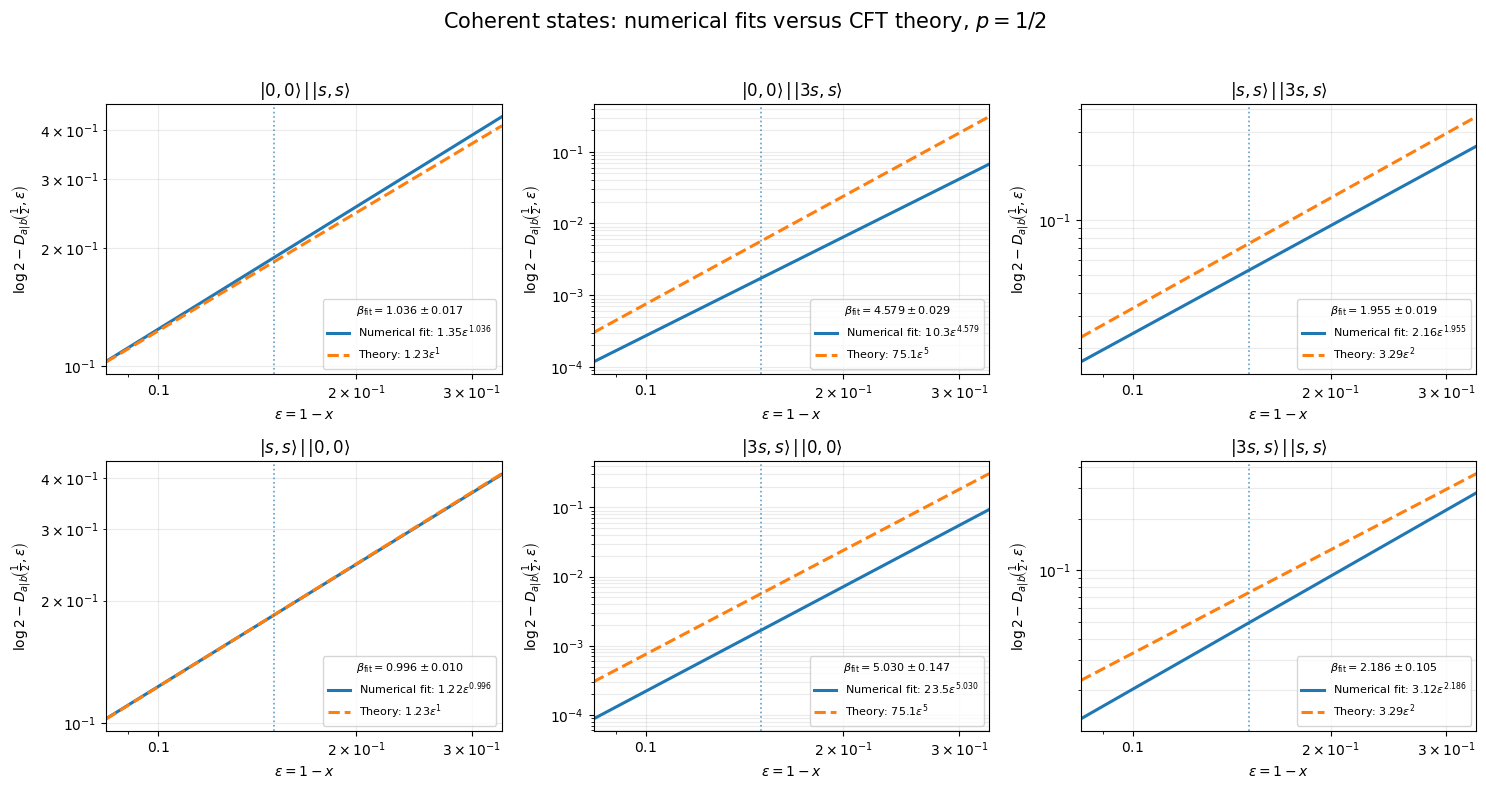
\includegraphics[width=1.0\textwidth]{rel_entropy_mixture_large_interval_numerics_theoryv3.png}
\end{figure}
\begin{figure}
        \centering
        % \captionsetup{justification=centering} 
        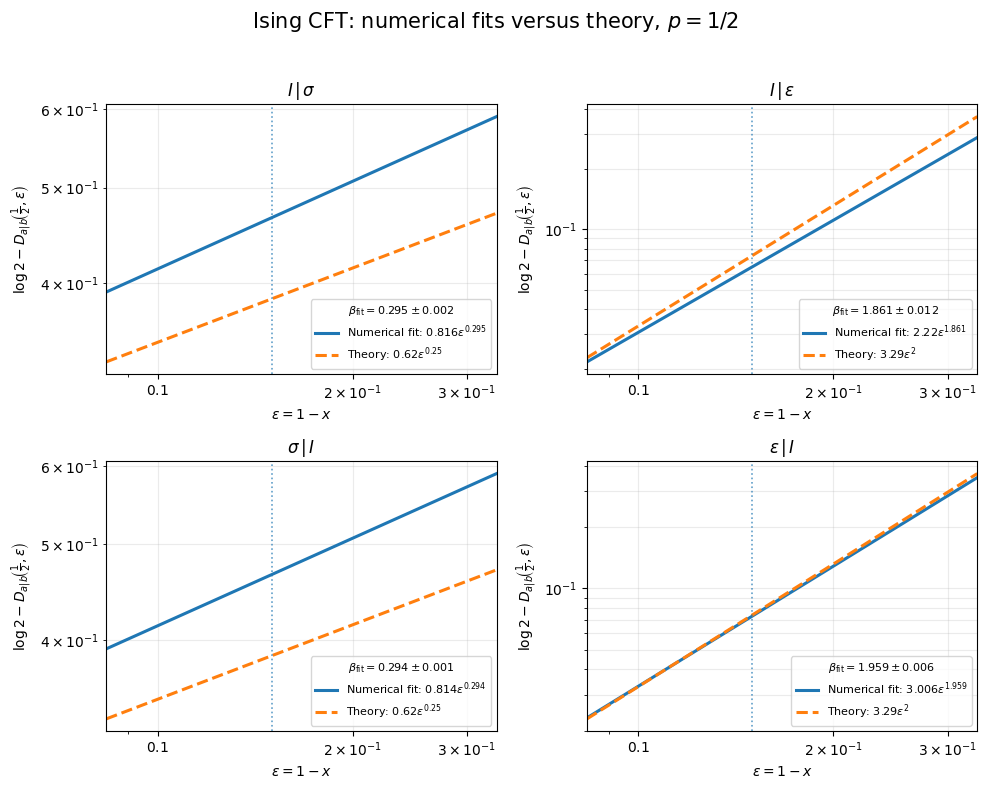
\includegraphics[width=0.7\textwidth]{rel_entropy_ising_mixture_large_interval_numerics_theoryv2.png}
        \caption{ Relative entropy in the Large Interval limit}
\end{figure}
\begin{figure}
        \centering
        % \captionsetup{justification=centering} 
        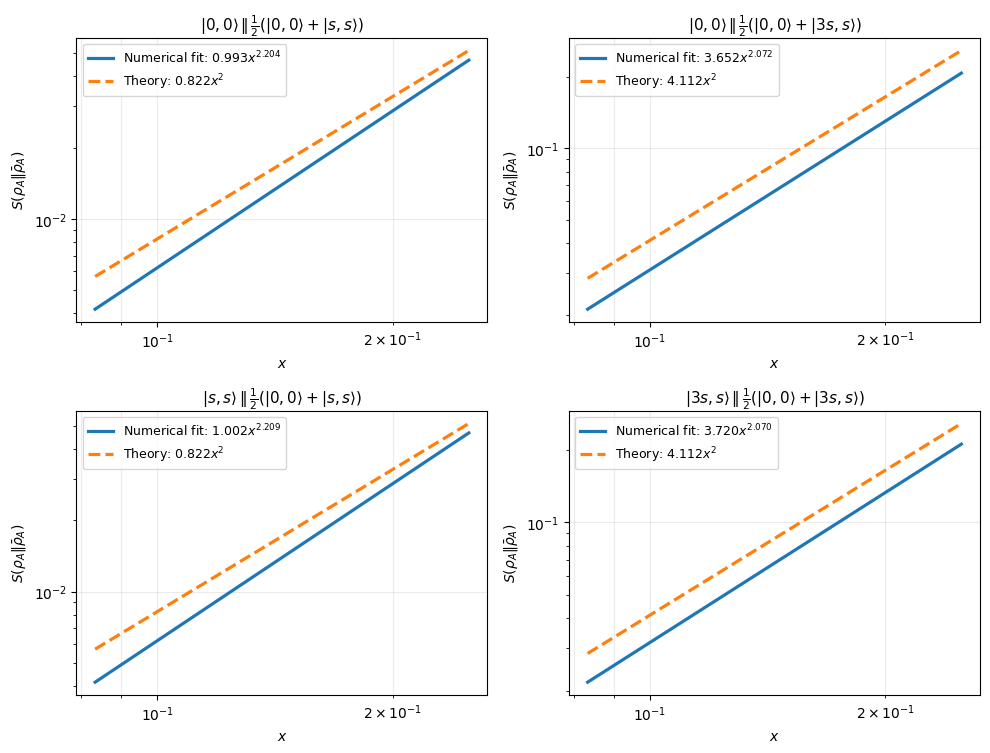
\includegraphics[width=1.0\textwidth]{rel_entropy_mixture_short_interval_numerics_theoryv5.png}
        \caption{ Relative entropy of Coherent states in the Small Interval limit}
\end{figure}

\subsection{Free boson}




\subsection{Minimal models}

% \section{Beyond small intervals}

% \subsection{Massless free boson}

%   In the free boson theory, the equation of motion is $\partial\bar{\partial}\phi(z,\bar{z})=0$ which means that the solutions to the equations of motion can be written as
%   \begin{align}
%     \phi(z,\bar{z})=\varphi(z)+\bar{\varphi}(\bar{z}).
%   \end{align}
%   The algebra of observables factors as the tensor product of a chiral and anti-chiral $U(1)$ current algebras with two–point functions 
% \[
% \langle \varphi(z)\varphi(0)\rangle=-\ln z, \qquad
% \langle \bar\varphi(\bar z)\bar\varphi(0)\rangle=-\ln \bar z, \qquad
% \langle \varphi(z)\bar\varphi(0)\rangle=0 .
% \]
% From the Schwinger-Dyson equations we know that up to contact terms $\partial\bar\partial\phi=0$ holds as an operator equation. This means that we can replace vertex operators in $\phi$ and $\partial_\mu \phi$ with their on-shell values up to contact terms. In free field theory, normal ordering keeps track of these contact terms. A general vertex operator of conformal weight $(\alpha ^2/2,\bar{\alpha}^2/2)$ is
% \begin{align}
% V_{\alpha,\bar{\alpha}}(z,\bar{z})&=:e^{i(\alpha\varphi(z)+\bar{\alpha}\bar{\varphi}(\bar{z}))}:=V_\alpha(z)V_{\bar\alpha}(\bar z)\nn\\
% V_\alpha(z)&=:e^{i \alpha\varphi(z)}:,\qquad V_{\bar\alpha}(\bar{z})=:e^{i \bar\alpha\bar\varphi(\bar z)}:
% \end{align}
% For now, we are assuming that the field is non-compact, i.e., $\phi:\mathbb{R}^{1,1}\to\mathbb{R}$, therefore $\alpha$ and $\bar{\alpha}$ are arbitrary real charges. We postpone a discussion of compact boson, the quantization of charge and winding until subsection \ref{sec:compact-boson}. 

% For linear functional of free fields we have
% \begin{align}
% :e^A::e^B:=e^{\langle A,B\rangle}\: :e^{A+B}:
% \end{align}
% Therefore, for the product of vertex operators we have the Wick contractions
% \[
% V_{\alpha,\bar\alpha}(z,\bar z)V_{\beta,\bar\beta}(0,0)
% =
% z^{\alpha\beta}\bar z^{\bar\alpha\bar\beta}V_{\gamma,\bar{\gamma}},\qquad \gamma=\alpha+\beta,\qquad \bar{\gamma}=\bar{\alpha}+\bar{\beta},
% % \nn\\
% % V_{}
% % :\exp\!\big(i\alpha\varphi(z)+i\beta\varphi(0)
% % +i\bar\alpha\bar\varphi(\bar z)+i\bar\beta\bar\varphi(0)\big): .
% \]

% \subsection{Vertex operators}

% The modular Hamiltonian of the vacuum on a cylinder of circumference $2\pi$ in the interval $(-x,x)$ is given by
% \begin{align}
% H_0&=\frac{(2\pi)^2}{2}\int_{-x}^x\frac{\cos(\pi y)-\cos(\pi x)}{\sin(\pi x)}T_{00}(x).
% \end{align}
% In a state with uniform energy density such as an exact energy eigenstate with dimension $h_\alpha$ on a cylinder of circumference $2\pi$ we have $\Delta T_{00}(y)=h/\pi$, and as a result
% \begin{align}
% \Delta H_\sigma\equiv \text{tr}((\rho_\alpha-\rho_0)H_0)=4h(1-\pi x\cot(\pi x))
% \end{align}
% For vertex operator with $h_\alpha=\bar{h}_\alpha$, a direct calculation shows that $S(\rho_\alpha)=S(\rho_0)$ which implies that 
% \begin{align}
% S(\rho_\alpha\|\rho_0)&=2\alpha^2(1-\pi x \cot(\pi x))=\Delta H_0\ .
% \end{align}
% As a result, we find $S(\rho_\alpha)=S(\rho_0)$ for all $x$ and $\alpha$. This suggests that $\rho_\alpha=V\rho_0V^\dagger$ for some unitary $V$. In fact, since $H_0$ generates a geometric flow in the Euclidean plane, it is indeed true that 
% \begin{align}
% V_{\alpha,\bar{\alpha}}(z,\bar{z})\sigma_0^{1/2}=\sigma_0^{1/2}V_{\alpha,\bar{\alpha}}(z',\bar{z}')
% \end{align}
% Then, since $\rho_\alpha=\sigma_0^{(1/2-x)}V_\alpha \sigma_0^{2x}V_{-\alpha}\sigma_0^{(1/2-x)}$, we have
% \begin{align}
%   \rho_\alpha=V_\alpha \sigma_0 V_\alpha^\dagger
% \end{align}
% and since $V_\alpha$ is unitary, we have
% \begin{align}
%   H_\alpha=V_\alpha \rho_0 V_\alpha^\dagger.
% \end{align}
% As a result,
% \begin{align}
% \tr(\rho_\alpha\log\rho_\beta)&=\tr(\rho_{\alpha-\beta}\log \rho_0)\nn\\
% S(\rho_\alpha\|\rho_\beta)&=S(\rho_{\alpha-\beta}\|\rho_0)=S(\rho_0\|\rho_{\alpha-\beta}).
% \end{align}
% In particular, this implies further that for a probability distribution $y_0+\sum_i y_i=0$ we have
% \begin{align}
% S(\rho_\alpha\|y_0\rho_\alpha+\sum_i y_i\rho_{\beta_i})&=S(\rho_0\|y_0\rho_0+\sum_i y_i\rho_{\beta_i-\alpha})
% \end{align}

% For an arbitrary energy eigenket we have
% \begin{align}
% S(\rho_h\|\rho_0)=S(\rho_h)-S(\rho_0)+4h(1-\pi x\cot(\pi x))
% \end{align}
% For instance, in the case of the eigenket generated by the action of $i\partial\varphi$ in the chiral free boson theory, we have
% \begin{align}
% &S(\rho_{i\partial\phi}\|\rho_0)=2(1-\pi x \cot(\pi x))+2\lb \log(2\sin(\pi x))+\psi_0(\csc(\pi x)/2)+\sin(\pi x)\rb
% \end{align}
% which implies the second term 
% \begin{align}
% 2\lb \log(2\sin(\pi x))+\psi_0(\csc(\pi x)/2)+\sin(\pi x)\rb
% \end{align}
% has the interpretation of $\Delta S$ as can be checked by the symmetry $x\to 1-x$. For these states we also have
% \begin{align}
% S(\rho_{i\partial \varphi}\|\rho_\beta)=S(\rho_{i\partial \varphi}\|\rho_0)+S(\rho_0\|\rho_\beta)
% \end{align}
% which requires an extra condition 
% \begin{align}
%   \tr((\rho_{i\partial \varphi}-\rho_0)(H_\beta-H_0))=0.
% \end{align}
% To derive this relation, we note that the current operator can be defined either as a spatial derivative of a vertex operator at zero charge, or the normal-ordered product of two vertex operators with unit and opposite charges
% \begin{align}
%   (i\partial \varphi)&=\frac{1}{\alpha}\partial_z V_\alpha|_{\alpha=0}=\partial_\alpha\partial_z V_\alpha|_{\alpha=0}\nn\\
%   (i\partial \varphi)&=\lim_{z\to 0} :V_\alpha(z)V_{-\alpha}(0):
% \end{align}
% Note that vertex operators of unit charge $\psi=e^{i\varphi}$ can be interpreted as a complex fermion:
% \begin{align}
% &\psi(z) \psi(w)=\frac{1}{(z-w)}:e^{i(\varphi(z)+\varphi(w))}=-\psi(w)\psi(z)\nn\\
% &(i\partial\varphi)(z)=J(z)=:\psi^\dagger\psi(z):
% \end{align}




% \NL{HERE}

% Expand the chiral/anti-chiral modes around the center of coordinates:
% \[
% \varphi(z)=\varphi(0)+z\,\partial\varphi(0)+\frac{z^2}{2}\partial^2\varphi(0)+O(z^3),
% \]

% \[
% \bar\varphi(\bar z)=
% \bar\varphi(0)+\bar z\,\bar\partial\bar\varphi(0)
% +\frac{\bar z^2}{2}\bar\partial^2\bar\varphi(0)+O(\bar z^3).
% \]
% and substituting into the exponent gives
% \begin{align}
% i\alpha\varphi(z)+i\beta\varphi(0)
% +i\bar\alpha\bar\varphi(\bar z)+i\bar\beta\bar\varphi(0)&=
% i\gamma\varphi(0)+i\bar\gamma\bar\varphi(0)
% +i\alpha z\,\partial\varphi(0)
% +i\bar\alpha\bar z\,\bar\partial\bar\varphi(0)\nn\\
% &\quad
% +\frac{i\alpha}{2}z^2\partial^2\varphi(0)
% +\frac{i\bar\alpha}{2}\bar z^2\bar\partial^2\bar\phi(0)
% +\cdots .
% \end{align}
% where we have defined the fused charges $
% \gamma=\alpha+\beta$ and $\bar\gamma=\bar\alpha+\bar\beta$.
% Therefore
% \[
% \begin{aligned}
% V_{\alpha,\bar\alpha}(z,\bar z)V_{\beta,\bar\beta}(0,0)
% &=
% z^{\alpha\beta}\bar z^{\bar\alpha\bar\beta}
% :\exp\!\Big(i\gamma\phi(0)+i\bar\gamma\bar\phi(0)\Big) \\
% &\qquad \times
% \exp\!\Big(
% i\alpha z\,\partial\phi(0)
% +i\bar\alpha \bar z\,\bar\partial\bar\phi(0) \\
% &\qquad\quad
% +\frac{i\alpha}{2}z^2\partial^2\phi(0)
% +\frac{i\bar\alpha}{2}\bar z^2\bar\partial^2\bar\phi(0)
% +\cdots
% \Big):\nn\\
% &=z^{\alpha\beta}\bar z^{\bar\alpha\bar\beta}
% :V_{\gamma,\bar\gamma}(0,0)e^Y:\nn\\
% Y&=i\alpha z\partial\phi(0)
% +i\bar\alpha\bar z\bar\partial\bar\phi(0)
% +\frac{i\alpha}{2}z^2\partial^2\phi(0)
% +\frac{i\bar\alpha}{2}\bar z^2\bar\partial^2\bar\phi(0)
% +\cdots .
% \end{aligned}
% \]
% Expanding $e^Y$ up to second order in derivatives we find
% \begin{align}
% e^Y
% &=
% 1
% +i\alpha z\,\partial\phi
% +i\bar\alpha \bar z\,\bar\partial\bar\phi
% +\frac{i\alpha}{2}z^2\partial^2\phi
% +\frac{i\bar\alpha}{2}\bar z^2\bar\partial^2\bar\phi\nn\\
% &\quad-\frac{\alpha^2}{2}z^2(\partial\phi)^2
% -\frac{\bar\alpha^2}{2}\bar z^2(\bar\partial\bar\phi)^2
% -\alpha\bar\alpha z\bar z\,\partial\phi\,\bar\partial\bar\phi
% +O(\text{level }3).
% \end{align}
% Combining everything, and defining $J=i \partial_z \varphi(z)$ and $\bar J=i \bar\partial_z \bar\varphi(z)$ we obtain
% \begin{align}
% V_{\alpha,\bar\alpha}(z,\bar z)V_{\beta,\bar\beta}(0,0)
% &=
% z^{\alpha\beta}\bar z^{\bar\alpha\bar\beta}
% \Big[
% V_{\gamma,\bar\gamma}(0,0)+:(\alpha zJ
% +\bar{\alpha}\bar{z} \bar{J})\,V_{\gamma,\bar\gamma}(0,0):\nn\\
% &\frac{1}{2}:\lb z^2(\alpha J'+\alpha^2 J^2)+\bar{z}^2(\bar{\alpha}\bar{J}'+\bar{\alpha}^2\bar{J}^2)\rb V_{\gamma,\bar\gamma}(0,0):\nn\\
% &+\alpha\bar{\alpha} z\bar{z}:J\bar{J} V_{\gamma,\bar\gamma}(0,0):
% +\cdots
% \Big].
% \end{align}
% In the case $\gamma=\alpha+\beta=0$ and $\bar{\gamma}=\bar{\alpha}+\bar{\beta}=0$, we have
% \begin{align}
% V_\alpha(z,\bar{z})V_{-\alpha}(0,0)&=(z\bar{z})^{-\alpha^2}\Big[ 1+\alpha :(z J+\bar{z}\bar{J})(0):\nn\\
% &\quad+\frac{\alpha}{2}:\lb z^2J+\bar{z}^2\bar{J}\rb(0):+\frac{\alpha^2}{2}:(z J+\bar{z}\bar{J})^2(0):+\cdots\Big]
% \end{align}
% We saw that the only operators that contribute for us have spin $h-\bar{h}$ is a multiple of $4$. Therefore, to this order the only operator that contributes to our correlator is 
% \begin{align}
% V_\alpha(z,\bar{z})V_{-\alpha}(0,0)=(z\bar{z})^{-\alpha^2}\lb 1+\alpha^2 \bar{z}\bar{z} (J\bar{J})(0,0)+\cdots\rb
% \end{align} 
% which has $h_p=\bar{h}_p=1$ and $C_\alpha=\alpha$. Therefore, $\Delta_L=2$ and
% \begin{align}
% S(\rho_\alpha\|y\rho_\alpha+(1-y)\rho_\beta)&=(\pi x)^4\frac{\sqrt{\pi}\Gamma(3)}{4\Gamma(7/2)}(1-y)^2(\alpha-\beta)^2+\cdots \nn\\
% &=\frac{4(\pi x)^4}{15}(1-y)^2(\alpha-\beta)^2+\cdots
% \end{align}
% At $y=1/2$ and $\alpha=0$ we find
% \begin{align}
%   S(\rho_0\|(\rho_0+\rho_\beta)/2)=\frac{(\pi x)^4\beta^2}{15}+\cdots
% \end{align}
% Note that this is $x^4$ order, not $x^2$ order. This is a consequence of the fact that the lowest primaries $J$ and $\bar{J}$ did not contribute because they are spin one. If instead of $V_{\alpha,\alpha}$ we considered chiral primaries, then $J$ would contribute at $x^2$ order \NL{Repeat the calculation in that case.}


% \subsection{Compact boson}\label{sec:compact-boson}

% For compact boson $\phi\sim \phi+2\pi R$ we have the momentum $m/R$ and winding modes $w R$ for $m,w\in\mathbb{Z}$, and left and right charges are
% \begin{align}
%   p_L=\frac{m}{R}+\frac{w}{2\pi R}, \qquad p_R=\frac{m}{R}-\frac{w}{2\pi R}.
% \end{align}
% The vertex operators are 
% \begin{align}
%   V_{m,w}(z,\bar{z})&=:e^{i(p_L\varphi(z)+p_R\bar\varphi(\bar{z}))}:,\qquad (h,\bar{h})=(p_L^2/2,p_R^2/2),\nn\\
%   \Delta&=h+\bar{h}=\frac{m^2}{R^2}+w^2 R^2,\qquad s=h-\bar{h}=m w.
% \end{align}
% The OPE is
% \begin{align}
%   V_{m,w}(z,\bar{z})V_{m',w'}(0,0)=z^{p_L p'_L}\bar{z}^{p_R p'_R}V_{m+m',w+w'}(0,0)\lb 1+\cdots\rb
% \end{align}
% We can use the Coulomb gas formalism to describe the operator content and OPE of all minimal models in terms of the OPE of vertex operators combined with screening charges. \NL{Do Ising model as an example}

% \subsection{Global symmetry}

% Symmetry resolved relative entropy

% In an exact energy eigenstate, the reduced density matrix is supposed to commute with the charge operator $Q$. There are superselection sectors, and the reduced state takes the form
% \begin{align}
%   &\rho=\oplus_q p_q \rho_q, \qquad \rho_q=\Pi_qr\rho_q \Pi_q,
% \end{align}
% where $\Pi_q$ is the projector onto the sector with charge $q$. 
% In the case of $U(1)$ current algebra, we have
% \begin{align}
%   &\Pi_q=\frac{1}{2\pi}\int d\alpha e^{-i\alpha Q}e^{i \pi q}
% \end{align}
% As explained in \cite{Capizzi} this project is given by the insertion of two vertex operators at the end points of the region. 



%   \subsection*{Operator Insertions on the Strip}

%   We perform the calculation on a strip of width $2\pi$, obtained via the
%   standard conformal mapping from the $n$-sheeted cylinder. The replica sheets are
%   indexed by $k = 0, \dots, n-1$.

%   The operator insertion points $t_{k}^{\pm}$ on the strip are:
%   \begin{equation}
%     t_{k}^{\pm}= \frac{2\pi k}{n}\pm \frac{\pi x}{n}
%   \end{equation}
%   where $x = l/R$ is the dimensionless interval size. For the correlator $\langle
%   \mathcal{O}_{\alpha}^{(q)}\mathcal{O}_{\beta}^{(p)}\rangle$ with $q=n-p$, the
%   operators are explicitly distributed as follows: On sheets $k=0, \dots, q-1$ ($\alpha$-sector)
%   we insert $V_{\alpha}$ at $t_{k}^{+}$ and $V_{-\alpha}$ at $t_{k}^{-}$, and on
%   sheets $k=q, \dots, n-1$ ($\beta$-sector) we insert $V_{\beta}$ at $t_{k}^{+}$
%   and $V_{-\beta}$ at $t_{k}^{-}$.

%   \subsection*{Special case}

%   For simplicity, focus on the special case $y=1/2$ so that we need to compute
%   \begin{eqnarray}
%     2^{-(n-1)}\frac{\tr(\rho_{0}(\rho_{0}+\rho_{\beta})^{n-1})}{\tr(\rho_{0}^{n})}&&=2^{-(n-1)}\Big(
%     1+(n-1)\frac{\tr(\rho_{0}^{n-1}\rho_{\beta})}{\tr(\rho_{0}^{n})}\nn\\
%     &&\quad+(n-1)\sum_{k=1}^{n-2}\frac{\tr(\rho_{0}^{k}\rho_{\beta}\rho_{0}^{n-1-k}\rho_{\beta})}{\tr(\rho_{0}^{n})}
%     \nn\\
%     &&\quad+(n-1)\sum_{k_1=1}^{n-3}\sum_{k_2=0}^{n-3-k_1}\frac{\tr(\rho_{0}^{k_1}\rho_{\beta}\rho_{0}^{k_2}\rho_{\beta}\rho_{0}^{n-3-k_1-k_2}\rho_{\beta})}{\tr(\rho_{0}^{n})}+\cdots\Big)
%   \end{eqnarray}
%   In this case, the first term $p=1$ gives
%   \begin{eqnarray}
%     &&\frac{\tr(\rho_{0}^{n-1}\rho_{\beta})}{\tr(\rho_{0}^{n})}=f(x)^{-\beta^2}\nn\\
%     &&f(x)\equiv (2\sin(\pi x/n)),
%   \end{eqnarray}
%   whereas the $p=2$ becomes
%   \begin{eqnarray}
%     &&\sum_{k=1}^{n-2}\frac{\tr(\rho_{0}^{k}\rho_{\beta}\rho_{0}^{n-1-k}\rho_{\beta})}{\tr(\rho_{0}^{n})}=f_1(x)^{-2\beta^2}
%     g_2(x;\beta)\nn\\
%     &&g_2(x;\beta) = \sum_{k=1}^{n-2} \left[
%     \frac{\sin^{2}\left(\frac{\pi k}{n}\right)}{\sin\left(\frac{\pi(k+x)}{n}\right)
%     \sin\left(\frac{\pi(k-x)}{n}\right)}
%     \right]^{\beta^2}\ .
%   \end{eqnarray}
%   For the $p=3$ term, we find
%   \begin{eqnarray}
%     \sum_{k_1=1}^{n-3}\sum_{k_2=0}^{n-3-k_1}\frac{\tr(\rho_{0}^{k_1}\rho_{\beta}\rho_{0}^{k_2}\rho_{\beta}\rho_{0}^{n-3-k_1-k_2}\rho_{\beta})}{\tr(\rho_{0}^{n})}=\cdots
%   \end{eqnarray}

% %  \section{General $x$}

  

%   \subsection*{Calculation of the correlator}

%   The correlation function for primary vertex operators $V_{Q}= :e^{i Q \phi}:$
%   is given by the product of distances raised to the power of the product of
%   their charges. The chordal distance on the strip is $d(t_{i}, t_{j}) = 2 \sin(\frac{t_{i}-
%   t_{j}}{2})$.
%   \begin{equation}
%     \langle \prod_{i}V_{Q_i}(t_{i}) \rangle \sim \prod_{i<j}\left[ 2 \sin\left( \frac{t_{i}-
%     t_{j}}{2}\right) \right]^{Q_i Q_j}
%   \end{equation}
%   \begin{itemize}
%     \item \textbf{Like charges} ($Q_{i}Q_{j}> 0$): The operators repel (regular
%       zero), leading to a positive exponent $+Q_{i}Q_{j}$.

%     \item \textbf{Opposite charges} ($Q_{i}Q_{j}< 0$): The operators attract (singular
%       pole), leading to a negative exponent $-|Q_{i}Q_{j}|$.
%   \end{itemize}

%   We have the following contributions:
%   \paragraph{1. Nearest Neighbor Interactions (Same sheet, same sector)}
%   These are the contractions between $t_{k}^{+}$ and $t_{k}^{-}$ on the same sheet.
%   \begin{itemize}
%     \item $\alpha$-sector ($q$ pairs): $(\alpha, -\alpha)$ separated by
%       $\Delta t = 2\pi x/n$.
%       \[
%         \implies \left( 2 \sin \frac{\pi x}{n}\right)^{-q \alpha^2}
%       \]

%     \item $\beta$-sector ($p$ pairs): $(\beta, -\beta)$ separated by
%       $\Delta t = 2\pi x/n$.
%       \[
%         \implies \left( 2 \sin \frac{\pi x}{n}\right)^{-p \beta^2}
%       \]
%   \end{itemize}
%   Putting the two together, we have
%   \begin{eqnarray}
%     \label{Nfunc} \mathcal{N}(q,p;x)=\left( 2 \sin \frac{\pi x}{n} \right)^{-(q\alpha^2+p\beta^2)}
%   \end{eqnarray}

%   \paragraph{2. Intra-sector Interactions (Different sheets, same sector)}
%   For the $\alpha$-sector, we sum over sheet separations $k = 1, \dots, q-1$. The
%   number of pairs at distance $k$ is $(q-k)$.
%   \begin{itemize}
%     \item Like charges $(\alpha, \alpha)$ and $(-\alpha, -\alpha)$:
%       \[
%         \text{Dist}= \frac{2\pi k}{n}\implies \text{Exp}= +\alpha^{2}\times 2
%       \]

%     \item Opposite charges $(\alpha, -\alpha)$: Two diagonals
%       $\frac{2\pi k}{n}\pm \frac{2\pi x}{n}$.
%       \[
%         \text{Dist}= \frac{2\pi (k\pm x)}{n}\implies \text{Exp}= -\alpha^{2}\text{
%         (each)}
%       \]
%   \end{itemize}
%   Collecting these terms for the $\alpha$ sector gives $[g(q;x)]^{\alpha^2}$:
%   \begin{eqnarray}
%     g(q;x) &= \prod_{k=1}^{q-1} \left(
%     \frac{\sin^{2}(\frac{\pi k}{n})}{\sin(\frac{\pi(k+x)}{n}) \sin(\frac{\pi(k-x)}{n})}
%     \right)^{q-k} \ .
%   \end{eqnarray}
%   The $\beta$ sector is identical with $q \to p$ and $\alpha \to \beta$, and we
%   have the overall contribution
%   \begin{eqnarray}
%     g(q;x)^{\alpha^2}g(p;x)^{\beta^2}\ .
%   \end{eqnarray}

%   \paragraph{3. Cross-sector Interactions}
%   Interactions between the $q$ $\alpha$-sheets and $p$ $\beta$-sheets yield
%   terms involving the product $\alpha \beta$. These collect into $[h(p,q;x)]^{\alpha\beta}$:
%   \begin{align}
%     \label{hfunct}h(q,p;x) & = \prod_{l=1}^{p}\prod_{k=1}^{q}\frac{\sin^{2}(\frac{\pi(k+l-1)}{n})}{\sin(\frac{\pi(k+l-1+x)}{n}) \sin(\frac{\pi(k+l-1-x)}{n})}
%   \end{align}

%   Putting all the pieces together, we find that the full correlator is
%   \begin{equation}
%     \label{eq:mixed_correlator}\langle \mathcal{O}_{\alpha}^{(q)}\mathcal{O}_{\beta}
%     ^{(p)}\rangle = \mathcal{N}(n-p,p;x) \left[ g(n-p;x) \right]^{\alpha^2}\left[
%     g(p;x) \right]^{\beta^2}\left[ h(n-p,p;x) \right]^{\alpha\beta}\ .
%   \end{equation}

%   We need to continue in $n$ analytically:
%   \begin{eqnarray}
%     \label{Fn} F(n)\equiv \text{tr}(\rho(\rho+\sigma)^{n-1}) &&= \sum_{p=0}^{n-1}
%     \binom{n-1}{p} \langle \mathcal{O}_{\alpha}^{(q)} \mathcal{O}_{\beta}^{(p)} \rangle
%   \end{eqnarray}

%   \subsection{Analytic continuation in $n$}

%   We consider the relative entropy $S(\rho_{\alpha}|| \sigma)$ where
%   $\sigma = y \rho_{\alpha}+ (1-y)\rho_{\beta}$ for excited coherent states in a
%   1+1D free boson CFT. The replica trick requires evaluating:
%   \begin{equation}
%     \text{tr}(\rho_{\alpha}\sigma^{n-1}) = \sum_{p=0}^{n-1}\binom{n-1}{p}y^{n-1-p}
%     (1-y)^{p}C_{n-p, p}
%   \end{equation}
%   where
%   $C_{n-p, p}= \langle \mathcal{O}_{\alpha}^{(n-p)}\mathcal{O}_{\beta}^{(p)}\rangle$
%   is the mixed correlator on the $n$-sheeted replica surface.

%   \paragraph{Step 1 Log-Sum expansion of the correlator:}
%   The correlator is a product of geometric functions $g$ and $h$. We focus
%   on the intra-sector term $\log g(p;x)$. For integer $p$, it is defined as:
%   \begin{equation}
%     \log g(p;x) = \sum_{k=1}^{p-1}(p-k) \left[ 2 \log d\left(\frac{k}{n}\right) -
%     \log d\left(\frac{k+x}{n}\right) - \log d\left(\frac{k-x}{n}\right) \right]
%   \end{equation}
%   where $d(y) = 2\sin(\pi y)$ is the distance between operator insertions. We
%   utilize the Fourier expansion for $\log \sin(\pi y)$:
%   \begin{equation}
%     \log \sin(\pi y) = -\log 2 - \sum_{m=1}^{\infty}\frac{\cos(2\pi m y)}{m}
%   \end{equation}
%   Substituting this into the potential $\mathcal{V}(k,x)$ inside the sum, the
%   constants cancel, yielding:
%   \begin{equation}
%     \mathcal{V}(k,x) = -2 \sum_{m=1}^{\infty}\frac{1}{m}\left[ 1 - \cos\left(\frac{2\pi
%     m x}{n}\right) \right] \cos\left(\frac{2\pi m k}{n}\right)
%   \end{equation}
%   The expression above has the advantage that it has separated the contribution
%   of $k$ from those of $x$, and we can now perform the sum over $k$.

%   \paragraph{Step 2 Sum over $k$:}
%   Following Section 6 of Calabrese, Cardy, and Tonni (2011), we perform the sum over
%   $k$ for each mode $m$:
%   \begin{equation}
%     \log g(p;x) = -2 \sum_{m=1}^{\infty}\frac{1 - \cos(2\pi m x/n)}{m}\sum_{k=1}^{p-1}
%     (p-k) \cos\left(\frac{2\pi m k}{n}\right)
%   \end{equation}
%   The inner sum $S_{m}(p) = \sum_{k=1}^{p-1}(p-k) \cos(k\theta_{m})$ is
%   evaluated using geometric series. For integer $p$ and $\theta_{m}=2\pi m/n$:
%   \begin{equation}
%     S_{m}(p) = \text{Re}\left[ \frac{p e^{i\theta_m}}{1-e^{i\theta_m}}- \frac{e^{i\theta_m}(1-e^{ip\theta_m})}{(1-e^{i\theta_m})^{2}}
%     \right]=\frac{-p}{2}+\frac{(1-\cos(p\theta_{m}))}{4\sin^{2}(\theta_{m}/2)},
%   \end{equation}
%   Therefore, we find
%   \begin{eqnarray}
%     \log g(p;x)=\sum_{m=1}^\infty \frac{1-\cos(\frac{2\pi m x}{n})}{m}\lb p-\frac{\sin^{2}(\pi
%     p m/n)}{\sin^{2}(\pi m/n)}\rb
%   \end{eqnarray}

%   Define the mode kernels
%   \begin{equation}
%     L(n,x):=\sum_{m=1}^{\infty}\frac{1-\cos(2\pi m x/n)}{m}, \qquad K_{m}(n,x):=
%     \frac{1-\cos(2\pi m x/n)}{2m\,\sin^{2}(\pi m/n)}. \label{eq:L-Km}
%   \end{equation}
%   to write
%   \begin{equation}
%     \log g(p;x)= p\,L(n,x)\;-\;\sum_{m=1}^{\infty}K_{m}(n,x)\,\bigl(1-\cos(p\theta
%     _{m})\bigr). \label{eq:logg-final}
%   \end{equation}
%   All $p$-independent pieces can be absorbed into $\Omega_{n}^{\rm (rest)}(x)$
%   later.

%   A technical note to keep in mind is that to make every rearrangement fully
%   justified, one may define all mode sums with a common Abel factor $e^{-\eps m}$
%   in the summand and take $\eps\to 0^{+}$ at the end. This guarantees absolute
%   and uniform convergence in intermediate steps.

%   Next, we move to the function $h(q,p;x)$ in (\ref{hfunct}) which includes a double
%   product over $(k,l)$ with $1\le k\le q$, $1\le l\le p$. Taking logs and using the
%   same log-sum representation as in we did for the $g$ function yields
%   \begin{equation}
%     \log h(q,p;x)=\sum_{r=1}^{n-1}w_{r}(p,q)\,V(r,x), \label{eq:logh-weighted}
%   \end{equation}
%   where $w_{r}(p,q)$ counts the number of pairs $(k,l)$ such that $k+l-1=r$.

%   It is convenient to evaluate the weighted cosine sum via generating functions.
%   Let $\theta$ be arbitrary and note
%   \begin{equation}
%     \sum_{r=1}^{n-1}w_{r}(p,q)e^{\ii r\theta}=\sum_{k=1}^{q}\sum_{l=1}^{p}e^{\ii(k+l-1)\theta}
%     =e^{-\ii\theta}\Big(\sum_{k=1}^{q}e^{\ii k\theta}\Big)\Big(\sum_{l=1}^{p}e^{\ii
%     l\theta}\Big). \label{eq:w-gen}
%   \end{equation}
%   Now specialize to the case $q=n-p$ and $\theta=\theta_{m}=2\pi m/n$. Using
%   \begin{equation}
%   \sum_{k=1}^{n-p}e^{\ii k\theta_m}=-e^{-\ii p\theta_m/2}\,\frac{\sin(p\theta_{m}/2)}{\sin(\theta_{m}/2)}
%   \quad\text{and}\quad
%   \sum_{l=1}^{p}e^{\ii l\theta_m}=e^{\ii(p+1)\theta_m/2}\,\frac{\sin(p\theta_{m}/2)}{\sin(\theta_{m}/2)},
%   \end{equation}
%   the right-hand side of \eqref{eq:w-gen} becomes real and equals
%   \begin{equation}
%     \sum_{r=1}^{n-1}w_{r}(p,n-p)\cos(r\theta_{m}) = -\left(\frac{\sin(p\theta_{m}/2)}{\sin(\theta_{m}/2)}
%     \right)^{2}= -\frac{1-\cos(p\theta_{m})}{2\sin^{2}(\theta_{m}/2)}. \label{eq:wcos-eval}
%   \end{equation}
%   Substituting \eqref{eq:wcos-eval} into \eqref{eq:logh-weighted} gives the exact
%   mode form
%   \begin{equation}
%     \log h(n-p,p;x)= 2\sum_{m=1}^{\infty}K_{m}(n,x)\,\bigl(1-\cos(p\theta_{m})\bigr
%     ), \label{eq:logh-final}
%   \end{equation}
%   with the \emph{same} $K_{m}(n,x)$ as in \eqref{eq:L-Km}.

%   We are now ready to put together all the pieces back into $C_{n-p,p}$. Using
%   \eqref{eq:logg-final} and \eqref{eq:logh-final}, we find
%   \begin{align}
%     \alpha^{2}\log g(q;x)+\beta^{2}\log g(p;x)+\alpha\beta\log h(q,p;x) & =(\alpha^{2}q+\beta^{2}p)\,L(n,x) \nonumber                                                             \\
%                                                                         & \quad-(\alpha-\beta)^{2}\sum_{m=1}^{\infty}K_{m}(n,x)\,\bigl(1-\cos(p\theta_{m})\bigr) \label{eq:combo}
%   \end{align}
%   where we have used a similar log-sum expansion for the function $\mathcal{N}$.
%   Absorbing all $p$-independent constants (including the $-(\alpha-\beta)^{2}\sum
%   _{m}K_{m}$ term) into $\Omega_{n}(x)$, we obtain
%   \begin{equation}
%     C_{n-p,p}(x) =\Omega_{n}(x)\,\Lambda_{\alpha}^{\,n-p}\,\Lambda_{\beta}^{\,p}\,
%     \exp\!\left[\sum_{m=1}^{\infty}a_{m}(n,x)\cos(p\theta_{m})\right], \label{eq:C-expcos}
%   \end{equation}
%   where
%   \begin{equation}
%     a_{m}(n,x)=(\alpha-\beta)^{2}\,K_{m}(n,x) =(\alpha-\beta)^{2}\,\frac{1-\cos(2\pi
%     m x/n)}{2m\,\sin^{2}(\pi m/n)}\ . \label{eq:am}
%   \end{equation}

%   \subsection{Fourier/Bessel expansion and definition of the $R$-modes}
%   Let $\theta:=\frac{2\pi p}{n}$ so that $\cos(p\theta_{m})=\cos(m\theta)$. Using
%   $e^{a\cos(m\theta)}=\sum_{r\in\mathbb{Z}}I_{r}(a)\,e^{\ii r m\theta}$ (modified
%   Bessel functions), we expand
%   \begin{equation}
%     \exp\!\left[\sum_{m\ge 1}a_{m}\cos(m\theta)\right] =\sum_{R\in\mathbb{Z}}W_{R}
%     (n,x;\alpha,\beta)\,e^{\ii R\theta}, \label{eq:WR-Fourier}
%   \end{equation}
%   where the coefficients are the (infinite) Bessel convolution
%   \begin{equation}
%     W_{R}(n,x;\alpha,\beta)= \sum_{\{r_m\}\,:\,\sum_{m\ge1} m r_m=R}\;\prod_{m\ge1}
%     I_{r_m}\!\big(a_{m}(n,x)\big), \qquad W_{-R}=W_{R}. \label{eq:WR-def}
%   \end{equation}
%   This allows us to rewrite
%   \begin{equation}
%     C_{n-p,p}(x) =\Omega_{n}\,\Lambda_{\alpha}^{\,n-p}\Lambda_{\beta}^{\,p}\; \sum
%     _{R\in\mathbb{Z}}W_{R}(n)\,e^{\ii \frac{2\pi R}{n}p}. \label{eq:C-R}
%   \end{equation}

%   Note that with an Abel regulator in the defining mode sums, the function of
%   $\theta$ in \eqref{eq:WR-Fourier} is real-analytic in a complex strip, which
%   implies exponential decay of $W_{R}$ and in particular
%   $\sum_{R}|W_{R}|<\infty$.

%   The expression in (\ref{eq:C-R}) has the advantage that if we can swap the sum
%   over $R$ with the sum over $p$, we can perform the $p$-sum explicitly. That is
%   our next step. {\bf I believe swapping the two sums can be justified using Abel regulators but I am not entirely sure!}

%   Plugging these back in \ref{Fn} and swapping the order of summation, we obtain
%   \begin{align}
%     F(n) & =\Omega_{n}\,\Lambda_{\alpha}\sum_{R\in\mathbb{Z}}W_{R}(n) \sum_{p=0}^{n-1}\binom{n-1}{p}\, (y\Lambda_{\alpha})^{n-1-p}\, \bigl((1-y)\Lambda_{\beta}e^{\ii2\pi R/n}\bigr)^{p}\nonumber \\
%          & = \Omega_{n}\,\Lambda_{\alpha}\sum_{R\in\mathbb{Z}}W_{R}(n)\, \Bigl(y\Lambda_{\alpha}+(1-y)\Lambda_{\beta}e^{\ii2\pi R/n}\Bigr)^{n-1}\ . \label{eq:F-R}
%   \end{align}

%   Next, we would like to argue that only the $R=0$ term in the expression above contrinutes
%   to the $n\to 1$ limit. To establish this, define $\eps=n-1$ and
%   \begin{equation}
%     A_{R}(n):=y\Lambda_{\alpha}+(1-y)\Lambda_{\beta}e^{\ii2\pi R/n},\qquad A_{0}:
%     =y\Lambda_{\alpha}+(1-y)\Lambda_{\beta}>0.
%   \end{equation}
%   Then \eqref{eq:F-R} reads
%   \begin{equation}
%     F(n)=\Omega_{n}\Lambda_{\alpha}\sum_{R\in\mathbb{Z}}W_{R}(n)\,A_{R}(n)^{\eps}
%     . \label{eq:F-eps}
%   \end{equation}

%   With an Abel regulator $W_{R}$ decays exponentially and has finite moments.
%   Expand the phase for $n=1+\eps$:
%   \begin{equation}
%     e^{\ii2\pi R/n}=e^{\ii2\pi R/(1+\eps)}=\exp\!\bigl(-\ii2\pi R\eps+O(R\eps^{2}
%     )\bigr),
%   \end{equation}
%   so $A_{R}(n)=A_{0}+\delta_{R}$ with $\delta_{R}=O(R\eps)$ for fixed $R$ and $\delta
%   _{-R}=\overline{\delta_R}$. Using
%   \begin{equation}
%     A_{R}^{\eps}=\exp\!\bigl(\eps\log(A_{0}+\delta_{R})\bigr)=A_{0}^{\eps}\left[1
%     +\eps\frac{\delta_{R}}{A_{0}}+O(\eps|\delta_{R}|^{2})\right],
%   \end{equation}
%   and the evenness $W_{-R}=W_{R}$, the potentially dangerous linear term $\sum_{R}
%   W_{R}\,\delta_{R}$ cancels at $O(\eps)$ (its leading part is odd/purely
%   imaginary), leaving only $O(\eps^{2})$ corrections after summing over $R$. Consequently,
%   after absorbing $\sum_{R}W_{R}$ into $\Omega_{n}$ (a $p$-independent normalization),
%   \begin{equation}
%     F(1+\eps)=\Omega_{1+\eps}\Lambda_{\alpha}\,A_{0}^{\eps}\bigl(1+O(\eps^{2})\bigr
%     ). \label{eq:F-asymp}
%   \end{equation}
%   Thus the $R\neq 0$ modes do not affect $\partial_{n}\log F(n)$ at $n=1$.

%   The replica prescription for the relative entropy is
%   \begin{equation}
%     S(\rho_{\alpha}\|\sigma_{y})= \left.\partial_{n}\Bigl(\log \tr(\rho_{\alpha}^{n}
%     )-\log \tr(\rho_{\alpha}\sigma_{y}^{n-1})\Bigr)\right|_{n=1}. \label{eq:S-replica}
%   \end{equation}
%   In the same framework one has $\tr(\rho_{\alpha}^{n})=\widetilde\Omega_{n}\,\Lambda
%   _{\alpha}^{\,n}$ so that $\partial_{n}\log \tr(\rho_{\alpha}^{n})|_{n=1}=\log\Lambda
%   _{\alpha}$ (all $\widetilde \Omega_{n}$ terms cancel against $\Omega_{n}$ in
%   the difference). Using \eqref{eq:F-asymp},
%   \begin{equation}
%     \left.\partial_{n}\log \tr(\rho_{\alpha}\sigma_{y}^{n-1})\right|_{n=1}=\log A
%     _{0}=\log\!\bigl(y\Lambda_{\alpha}+(1-y)\Lambda_{\beta}\bigr).
%   \end{equation}
%   Therefore
%   \begin{equation}
%     S(\rho_{\alpha}\|\sigma_{y})=\log\Lambda_{\alpha}-\log\!\bigl(y\Lambda_{\alpha}
%     +(1-y)\Lambda_{\beta}\bigr) = -\log\!\left[y+(1-y)\frac{\Lambda_{\beta}}{\Lambda_{\alpha}}
%     \right]. \label{eq:S-Lambda}
%   \end{equation}

%   For coherent-state excitations in the free boson CFT one may identify
%   \begin{equation}
%     \frac{\Lambda_{\beta}}{\Lambda_{\alpha}}=e^{-S(\alpha\|\beta)}, \qquad S(\alpha
%     \|\beta)=(\alpha-\beta)^{2}K(x), \qquad K(x)=1-\pi x\cot(\pi x). \label{eq:Salpha}
%   \end{equation}
%   Substituting \eqref{eq:Salpha} into \eqref{eq:S-Lambda} gives the final answer
%   \begin{equation}
%     \boxed{ S\!\left(\rho_\alpha\,\Big\|\,y\rho_\alpha+(1-y)\rho_\beta\right) = -\log\!\left( y+(1-y)\exp\!\big[-(\alpha-\beta)^2(1-\pi x\cot(\pi x))\big] \right). }
%     \label{eq:S-final}
%   \end{equation}

% \subsection{Current algebra: Symmetry resolved relative entropy}



%   \section{Consistency tests}
%   \label{sec:tests}

%   Let $s:=(\alpha-\beta)^{2}K(x)\ge 0$ and $a:=e^{-s}\in(0,1]$ so that
%   \begin{eqnarray}
%     S(y)\equiv S\!\left(\rho_\alpha\,\Big\|\,y\rho_\alpha+(1-y)\rho_\beta\right)=-\log\lb
%     y+(1-y)a\rb=-\log(a+(1-y)a)
%   \end{eqnarray}
%   We are gonna test the following limits:
%   \begin{itemize}
%     \item \textbf{Identical states:}
%       $\alpha=\beta\Rightarrow s=0\Rightarrow a=1\Rightarrow S(y)=0$ as expected.

%     \item \textbf{No mixing:} $S(1)\to 0$ as expected and
%       $S(0)=S(\alpha\|\beta)$ as expected. Therefore, we can write
%       \begin{eqnarray}
%         e^{-S(y)}=y e^{-S(1)}+(1-y)e^{-S(0)}\ .
%       \end{eqnarray}

%     \item \textbf{Much heavier state:}
%       $s\to\infty\Rightarrow a\to 0\Rightarrow S_{y}\to -\log y$.
%   \end{itemize}

%   Next, we test the following properties:

%   \begin{itemize}
%     \item \textbf{Positivity:} Since $y\le a+y(1-a)\le 1$, we have $0\le S(y)\le
%       -\log y$ as required fo r relative entropy.

%     \item \textbf{Convexity in $y$:} Taking derivatives with respect to $y$
%       \begin{equation}
%         S'(y)= -\frac{1-a}{a+y(1-a)}\le 0, \qquad S''(y)=\frac{(1-a)^{2}}{(a+y(1-a))^{2}}
%         \ge 0.
%       \end{equation}
%       Thus $S(y)$ is decreasing and convex in the mixing parameter $y$ (strictly
%       convex if $s>0$), consistent with the general theorem that $S(\rho\|\sigma)$
%       is convex in $\sigma$.

%     \item \textbf{Monotonicity and concavity in $s$:} Treating $S$ as a function
%       of $s$:
%       \begin{equation}
%         \frac{\partial S}{\partial s}=\frac{(1-y)e^{-s}}{y+(1-y)e^{-s}}\ge 0, \qquad
%         \frac{\partial^{2}S}{\partial s^{2}}=-\frac{y(1-y)e^{-s}}{(y+(1-y)e^{-s})^{2}}
%         \le 0.
%       \end{equation}
%       So $S$ increases with $s$ but is concave in $s$, consistent with
%       saturation at $-\log y$. A direct derivative gives the derivative of relative
%       entropy in region size
%       \begin{equation}
%         K'(x)=\frac{\pi}{\sin^{2}(\pi x)}\left(\pi x-\frac{1}{2}\sin(2\pi x)\right
%         )>0 \qquad \text{for }x\in(0,1),
%       \end{equation}
%       since $\sin u<u$ for $u>0$. Thus $K(x)$ (and therefore $S$) is increasing
%       in $x$ for $\alpha\neq\beta$, as expected from data processing.
%   \end{itemize}

%   Finally, we note that in the small interval limit $x\ll 1$ we have
%   \begin{equation}
%     K(x)=1-\pi x\cot(\pi x)=\frac{\pi^{2}}{3}x^{2}+\frac{\pi^{4}}{45}x^{4}+O(x^{6}
%     ).
%   \end{equation}
%   Hence
%   \begin{equation}
%     S(y)= (1-y)\,(\alpha-\beta)^{2}\frac{\pi^{2}}{3}x^{2}+O(x^{4}).
%   \end{equation}
%   The relative entropy vanishes as $x^{2}$ for small intervals, as expected.

%   \subsection*{Alternative analytic continuation}
%   \label{sec:small-n1} An alternative analytic continuation follows from observing
%   that since we are interested in small $n-1$, and the sum over
%   $p=1,\cdots , n-1$, we linearize our functions in $p$ and discard higher order
%   terms:
%   \begin{equation}
%     S_{m}(p)= -\frac{p}{2}+\frac{1-\cos(p\theta_{m})}{4\sin^{2}(\theta_{m}/2)}= -
%     \frac{p}{2}+O(p^{2}). \label{eq:Sm-smallp}
%   \end{equation}
%   Expanding the $g$ function in $n=1+\epsilon$ results in
%   \begin{equation}
%     \log g(p;x)=p\,L(n,x)+O(p^{2})=p\,L(n,x)+O(\eps^{2}),
%   \end{equation}
%   uniformly over the relevant range $p\in\{0,\dots,n-1\}$. This reproduces the linear-in-$p$
%   structure that one would obtain by keeping only the ``smooth'' term $S_{m}(p)\approx
%   -p/2$ and effectively discarding the oscillatory $\cos(p\theta_{m})$ piece at this
%   order. While this results in a different analytic continuation than what we
%   computed above, the $n\to 1$ limit gives the same result, and the same final
%   expression \eqref{eq:S-final} for relative entropy.

  %------------------------------------------------------------
  % Appendix-style writeup: pole-matching analytic continuation
  %------------------------------------------------------------

  \section{Information-theoretic interpretation}

  \appendix
\section{Analytic continuation of the replica sum with a phase}
\label{app:analytic-continuation}

In this appendix we derive the analytic continuation in the replica index
of the sum
\begin{align}
\mu(n)&=\sum_{p=1}^{n-1}\frac{(n-p)e^{-2\pi i \kappa_n p}}{\sin^{2\Delta}\!\left(\frac{\pi p}{n}\right)}\nn\\
e^{-2\pi i \kappa_n}&:=r_n(x):=(y^{-1}-1)D_n(1-x)=(y^{-1}-1)\lb\frac{n\sin(\pi (1-x)/n)}{\sin(\pi (1-x))} \rb^{4(h_\alpha-h_\beta)},
\end{align}
and compute its derivative at $n=1$. First note that for all positive integer $n$ the function $D_n(1-x)\geq 1$, which means that for $h_\beta\geq h_\alpha$ and $0\leq y\leq 1/2$ the function $r_n(x)$ is real, and bounded above by one:
\begin{align}
  \forall\: 0\leq y\leq 1/2, h_\alpha\leq h_\beta: \qquad 0\leq r_n(x)\leq 1,   
\end{align}
We are going to focus on this case. Redefining $p\to n-p$ we have
\begin{align}
\mu(n)=r_n(x)^{n}\sum_{p=1}^{n-1}\frac{p e^{2\pi i \kappa_n p}}{\sin^{2\Delta}\left(\frac{\pi p}{n}\right)}.
\end{align}


Our derivation of the analytic continuation $\mu(1)$ and $\mu'(1)$ in this limit follows closely the
method used by Cardy, Tonni and collaborators\cite{calabrese2011entanglement}, based on Fourier analysis
and Carlson's theorem.

\subsection{Fourier coefficients of the sine kernel}

Define the periodic kernel
\begin{equation}
f(x)=\sin^{-2\Delta}(\pi x).
\end{equation}
Its Fourier coefficients are
\begin{equation}
f_\Delta(m)=\int_0^1 dx\,\frac{e^{-2\pi i m x}}{\sin^{2\Delta}(\pi x)},
\qquad m\in\mathbb Z .
\end{equation}
Using the standard beta-function integral one finds
\begin{equation}
f_\Delta(m)=
\frac{2^{2\Delta}\Gamma(1-2\Delta)e^{-i\pi m}}
{\Gamma(1-\Delta+m)\Gamma(1-\Delta-m)} .
\end{equation}
For analytic continuation it is convenient to introduce a holomorphic
interpolation of the positive Fourier coefficients to complex $m$,
\begin{equation}\label{eq: Fourier coeff of csc^2Delta}
g_\Delta(m)=c_\Delta\,\frac{\Gamma(m+\Delta)}{\Gamma(m+1-\Delta)},
\qquad
c_\Delta=\frac{2^{2\Delta}\Gamma(1-2\Delta)\sin(\pi\Delta)}{\pi}.
\end{equation}
This function reproduces the discrete data
\(
g_\Delta(m)=f_\Delta(m)
\)
for integer $m\ge0$ and satisfies the growth conditions required for the
application of Carlson's theorem.

\subsection{Analytic continuation of the replica sum}

Following the Poisson-resummation strategy used in
\cite{calabrese2011entanglement}, the analytic continuation of the replica sum can be
written as
\begin{equation}
S_n(k_0,\Delta)=
\frac{1}{2}\sum_{m\ge1}\big[n\,g(nm-\kappa_n)-g(m-\kappa_n)\big]
+
\sum_{m\ge0}\big[n\,g(-nm-\kappa_n)-g(-m-\kappa_n)\big],
\end{equation}
where
\begin{equation}
\kappa_n=-\frac{n k_0}{2\pi}.
\end{equation}

This expression reproduces the original discrete sum for integer $n$ and
provides its analytic continuation.

% \subsection{Derivative at $n=1$}
\subsection{\texorpdfstring{Derivative at $n=1$}{Derivative at n=1}}

To compute the derivative at $n=1$ we differentiate term by term.  In the
strip $0<\Re\Delta<1/2$ the series converge absolutely, allowing the
interchange of differentiation and summation.  One obtains
% \begin{equation}
% \partial_n S_n\big|_{n=1}=
% \sum_{m=1}^\infty\big[g(m-\kappa)+m g'(m-\kappa)\big]
% +
% \sum_{m=0}^\infty\big[g(m+\kappa)-m g'(m+\kappa)\big],
% \end{equation}
\begin{align}
\partial_n S_n\big|_{n=1}&=\frac{1}{2}
\sum_{m=1}^\infty\big[g(m-\kappa)+m g'(m-\kappa)\big]
+
\sum_{m=0}^\infty\big[g(-m-\kappa)-m g'(-m-\kappa)\big],  \nn \\
% \p_n S_n \big|_{n=1} 
&= \frac{1}{2}
\sum_{m=1}^\infty\big[g(m-\kappa)+m g'(m-\kappa)\big] + \sum_{m=0}^\infty\big[g(m-\kappa)+m g'(m-\kappa)\big].
\end{align}
where $\kappa=\kappa_{n=1}=-k_0/(2\pi)$.

\subsection{Integral representation}

To evaluate these sums we use the beta-function identity
\begin{equation}
\frac{\Gamma(z+\Delta)}{\Gamma(z+1-\Delta)}
=
\frac{1}{\Gamma(1-2\Delta)}
\int_0^1 dt\, t^{z+\Delta-1}(1-t)^{-2\Delta},
\end{equation}
valid for $0<\Re\Delta<1/2$.

This gives
\begin{equation}
g(z)=A_\Delta\int_0^1 dt\, t^{z+\Delta-1}(1-t)^{-2\Delta},
\qquad
A_\Delta=\frac{2^{2\Delta}\sin(\pi\Delta)}{\pi}.
\end{equation}

Differentiating,
\begin{equation}
g'(z)=A_\Delta\int_0^1 dt\, t^{z+\Delta-1}(1-t)^{-2\Delta}\ln t .
\end{equation}

Substituting these expressions into the derivative formula and
interchanging the order of summation and integration we obtain
% \begin{equation}
% \partial_n S_n\big|_{n=1}=
% A_\Delta\int_0^1 dt (1-t)^{-2\Delta}
% \left[
% \sum_{m=1}^\infty t^{m-\kappa+\Delta-1}(1+m\ln t)
% +
% \sum_{m=0}^\infty t^{m+\kappa+\Delta-1}(1-m\ln t)
% \right].
% \end{equation}
\begin{equation}
\partial_n S_n\big|_{n=1}=
\frac{A_\Delta}{2}\int_0^1 dt (1-t)^{-2\Delta}
\left[
\sum_{m=1}^\infty t^{m-\kappa+\Delta-1}(1+m\ln t)
+
\sum_{m=0}^\infty t^{m-\kappa+\Delta-1}(1+m\ln t)
\right].
\end{equation}

\subsection{Performing the sums}

Using the geometric-series identities
\begin{align}
\sum_{m=1}^\infty t^m &=\frac{t}{1-t},\\
\sum_{m=1}^\infty m t^m &=\frac{t}{(1-t)^2},\\
\sum_{m=0}^\infty t^m &=\frac{1}{1-t},
\end{align}
the sums can be evaluated explicitly.  This yields
% \begin{equation}
% \partial_n S_n\big|_{n=1}=
% A_\Delta\int_0^1 dt
% \left[
% \frac{t^{\Delta-\kappa}+t^{\Delta+\kappa-1}}{(1-t)^{2\Delta+1}}
% +
% \frac{(t^{\Delta-\kappa}-t^{\Delta+\kappa})\ln t}{(1-t)^{2\Delta+2}}
% \right].
% \end{equation}
\begin{equation}
\partial_n S_n\big|_{n=1}=
\frac{A_\Delta}{2}\int_0^1 dt
\left[
\frac{t^{\Delta-\kappa}+t^{\Delta-\kappa-1}}{(1-t)^{2\Delta+1}}
+
\frac{2t^{\Delta-\kappa}\ln t}{(1-t)^{2\Delta+2}}
\right].
\end{equation}

\subsection{Final evaluation}

The remaining integrals can be evaluated using
\begin{align}
\int_0^1 dt\, t^{a-1}(1-t)^{b-1}&=B(a,b),\\
\int_0^1 dt\, t^{a-1}(1-t)^{b-1}\ln t
&=B(a,b)\,[\psi(a)-\psi(a+b)].
\end{align}

After straightforward algebra we obtain
% \begin{equation}
% \begin{aligned}
% \partial_n S_n(k_0,\Delta)\big|_{n=1}
% &=
% \frac{2^{2\Delta}\sin(\pi\Delta)}{\pi}
% \Big[
% B(1+\Delta-\kappa,-2\Delta)
% +
% B(\Delta+\kappa,-2\Delta)
% \\
% &\quad
% +
% B(1+\Delta-\kappa,-1-2\Delta)
% (\psi(1+\Delta-\kappa)-\psi(-\Delta-\kappa))
% \\
% &\quad
% -
% B(1+\Delta+\kappa,-1-2\Delta)
% (\psi(1+\Delta+\kappa)-\psi(\kappa-\Delta))
% \Big],
% \end{aligned}
% \end{equation}
\begin{equation}
\begin{aligned}
\partial_n S_n(k_0,\Delta)\big|_{n=1}
&=
\frac{2^{2\Delta-1}\sin(\pi\Delta)}{\pi}
\Big[
B(1+\Delta-\kappa,-2\Delta)
+
B(\Delta\JM{-}\kappa,-2\Delta)
\\
&\quad
+ 2
B(1+\Delta-\kappa,-1-2\Delta)
(\psi(1+\Delta-\kappa)-\psi(-\Delta-\kappa))\Big],
% \\
% &\quad
% -
% B(1+\Delta+\kappa,-1-2\Delta)
% (\psi(1+\Delta+\kappa)-\psi(\kappa-\Delta))
% \Big],
\end{aligned}
\end{equation}
with
\begin{equation}
\kappa=-\frac{k_0}{2\pi}.
\end{equation}

This expression gives the analytically continued derivative of the replica
sum at $n=1$.

Now if we set $\kappa = 0$, we get the desired result. This can be shown by using the identities of Gamma and digamma functions.
\begin{align}
    \mu_0'(1) =  \p_nS_n(k_0 = 0,\Delta)\big|_{n=1}& = \frac{2^{2\Delta -1}\sin (\pi \Delta)}{\pi} \Big[ \frac{\Gamma(\Delta +1) \Gamma(-2\Delta)}{\Gamma(-\Delta +1)} + \frac{\Gamma(\Delta) \Gamma(-2\Delta)}{\Gamma(-\Delta)} \nn \\
    &\qquad \qquad \qquad+ 2B(\Delta + 1, -2\Delta -1) (\psi(1+ \Delta) - \psi(-\Delta))\Big]  
    \nn \\
    & = \frac{2^{2\Delta -1}\sin (\pi \Delta)}{\pi}  \Big[ \frac{\Delta \Gamma(\Delta)\Gamma(-2\Delta)}{-\Delta \Gamma(-\Delta) } + \frac{\Gamma(\Delta)\Gamma(-2\Delta)}{\Gamma(-\Delta)}\nn \\
    &\qquad \qquad \qquad+ \frac{2\Gamma(\Delta + 1)\Gamma(-2\Delta - 1)}{\Gamma(-\Delta)}(-\pi \cot (\pi \Delta))
    \Big]\nn \\
    &= 2^{2\Delta}\cos (\pi \Delta) \Big[  \frac{\Gamma(\Delta + 1)\Gamma(-2\Delta -1)}{\frac{\pi }{\sin(\pi \Delta)\Gamma(1+\Delta)}}\Big]\nn \\
    &=  \frac{2^{2\Delta - 1}} {\pi}\sin(2\pi \Delta) (\Gamma(1+\Delta))^2 \Gamma(-2\Delta - 1) \nn \\
    &= 2^{2\Delta - 1}  \frac{(\Gamma(1+\Delta))^2}{\Gamma(2+2\Delta)} \nn \\
    &= \frac{2^{2\Delta -1}(\Gamma(1+\Delta))^2}{\Big(\frac{\Gamma(1+\Delta)\Gamma(\Delta + 3/2)}{\sqrt{\pi} 2^{1-2(1+\Delta)}}\Big)} \nn \\
    &= \frac{\sqrt{\pi }\Gamma(1+\Delta)}{4 \Gamma(\Delta + 3/2)}.
\end{align}

where we used the following identities,
\begin{align*}
    \psi(1+\Delta) - \psi(-\Delta) &= -\pi \cot(\pi \Delta)\nn \\
    \Gamma(1+z)\Gamma(-z) &= -\frac{\pi}{\sin(\pi z)} \nn \\ 
    \Gamma(z)\Gamma(z+1/2)& = 2^{1-2z}\sqrt{\pi}\Gamma(2z)
\end{align*}

% \JM{The result above should match with $\mu_0'(1)= \frac{2^{-2\Delta_L}\sqrt{\pi}\Gamma(\Delta_L+1)}{4\Gamma(\Delta_L+3/2)}$, however from the result above, $\partial_n S_n(k_0 =0,\Delta)\big|_{n=1} = 0$. This can be shown by taking $\kappa =0$, the third and fourth term cancel, and we are left with
% \begin{align}
%     B(1+\Delta - ,-2\Delta) + B(\Delta + ,-2\Delta) &= \frac{\Gamma(1+\Delta)\Gamma(-2\Delta)}{\Gamma(1-\Delta)} + \frac{\Gamma(\Delta)\Gamma(-2\Delta)}{\Gamma(-\Delta)} \nn \\
%     &= \frac{\Delta \Gamma(\Delta) \Gamma(-2\Delta)}{-\Delta \Gamma(-\Delta)} + \frac{\Gamma(\Delta)\Gamma(-2\Delta)}{\Gamma(-\Delta)} \nn \\
%     &= 0.
% \end{align}
% }

% \section{Analytic continuation of $\mu_1(n)$ using Cardy, Tonni and collaborators}
\section{\texorpdfstring{Analytic continuation of $\mu_1(n)$ using Cardy, Tonni and collaborators}
{Analytic continuation of mu1(n) using Cardy, Tonni and collaborators}}
Cardy, Tonni and collaborators analyticaaly continued the sum $S_2(n)$ and its derivative at $n=1$ using Carlson's theorem. They analytically continued 
\begin{align*}
    S_2(n) = \frac{1}{2}\sum_{j=1}^{n-1} \frac{1}{\big[\sin^2\lb \frac{2\pi j}{2n} \rb\big]^\alpha} \equiv \frac{1}{2}\sum_{k = -\infty}^{\infty}[ng(nk)-g(k)]
\end{align*}
where $g(k)$ is the analytic continuation of the Fourier modes $f(k)$ of $\lb\sin^2(u/2)\rb^{-\alpha}$. However, for $\mu_1(n)$, we want the analytic continuation of the sum involving,
\begin{align}
    \mu_1(n) = \frac{1}{2}\sum_{p=1}^{n-1}\frac{p^2}{\lb \sin^2\lb \frac{\pi p}{n}\rb \rb^\Delta}
\end{align}
For this higher moment, we will consider the Fourier modes of the generating function,
\begin{align}
    \frac{e^{-2i\kappa u }}{(\sin^2(u))^\Delta}
\end{align}
We can take two derivatives with respect to $\kappa$ to obtain the desired sum, and set $\kappa= 0$ in the end. 
By adding this extra source term, we replace $m$ with $m + \kappa$ in eq.~[\ref{eq: Fourier coeff of csc^2Delta}], and obtain,
\begin{align}
    g(m,\kappa) = c_\Delta \frac{\Gamma(1-2\Delta) \Gamma(m + \kappa + \Delta)}{\Gamma(m+\kappa + 1 - \Delta)}
\end{align}
Then the sum is given by,
\begin{align}
    \mu_1(n) &= -\frac{1}{4}\frac{1}{2}\p_\kappa^2 \left[ \sum_{m\geq 1} \lb ng(n(m+\kappa)) - g(m+\kappa) \rb+ \sum_{m\geq 0}\lb ng(-nm+n\kappa) - g(-m-\kappa) \rb \right] \nn \\
    & = -\frac{1}{8} \left[ \sum_{m\geq 1}\lb n^3 g''(n(m+\kappa)) - g''(m+\kappa) \rb +\sum_{\geq 0}\lb n^3g''(-nm+n\kappa) -g''(-m-\kappa) \rb  \right].
\end{align}
% where in the second step, we used $g(-m) = g(m)$ for integer $m$.
Then, we take the derivative with respect to $n$, and take the limit $n=1$ and $\kappa = 0$, along with using the reflection $g(-m) = g(m)$ for integer $m$, to obtain,
\begin{align}
    \p_n \mu_1 \big|_{n=1,\kappa = 0} = -\frac{1}{8} \left[ \sum_{m\geq 1} \lb 3g''(m) + mg'''(m) \rb  + \sum_{m\geq 0}\lb  3g''(m) + mg'''(m) \rb\right]
\end{align}
Making use of the following integral representation of the analytically continued Fourier modes, 
\begin{align}
    g(m+\kappa) &= A_\Delta \int_0^1 dt \, t^{m+\kappa + \Delta - 1} (1-t)^{-2\Delta} \\
    g'(m+\kappa) &= A_\Delta \int_0^1 dt \, t^{m+\kappa + \Delta - 1} (1-t)^{-2\Delta} \ln t \\ 
    g''(m+\kappa) &= A_\Delta \int_0^1 dt \, t^{m+\kappa + \Delta - 1} (1-t)^{-2\Delta} (\ln t)^2 \\ 
    g'''(m+\kappa) &= A_\Delta \int_0^1 dt \, t^{m+\kappa + \Delta - 1} (1-t)^{-2\Delta} (\ln t)^3 \\ 
\end{align}
We obtain,
\begin{align}
    \p_n \mu_1(n)\big|_{n=1} &= -\frac{A_\Delta}{8} \Big( \sum_{m\geq 1} 3 \int_0^1 dt \, t^{m+\kappa + \Delta - 1}(1-t)^{-2\Delta} (\ln t)^2  + \sum_{m\geq 1} m\int_0^1 dt \, t^{m+\kappa + \Delta - 1}(1-t)^{-2\Delta} (\ln t)^3 \\
    & \qquad \qquad  \sum_{m\geq 0 }3 \int_0^1 dt \, t^{m+\kappa + \Delta - 1}(1-t)^{-2\Delta} (\ln t)^2  +  \sum_{m\geq 1} m\int_0^1 dt \, t^{m+\kappa + \Delta - 1}(1-t)^{-2\Delta} (\ln t)^3
    \Big)
\end{align}
Doing the sum over $m$, we get,
\begin{align}
    \p_n \mu_1(n)\big|_{n=1} &= -\frac{A_\Delta}{8} \Bigg( 3\int_0^1 dt \, \frac{t^{\kappa + \Delta} (\ln t)^2}{(1-t)^{2\Delta + 1}} + 2\int_0^1  dt \, \frac{t^{\kappa + \Delta }(\ln t)^3}{(1-t)^{2\Delta + 2}} +  3\int_0^1 dt \, \frac{t^{\kappa + \Delta-1} (\ln t)^2}{(1-t)^{2\Delta + 1}} \Bigg)
\end{align}
We use the following integrals,
\begin{align}
    \int_0^1 dt \, t^{a-1} (1-t)^{b-1}(\ln t)^2 &= B(a,b) \left[ \lb \psi(a) - \psi(a+b) \rb^2 + \lb \psi_1(a) - \psi_1(a+b) \rb  \right] \\ 
    \int_0^1 dt \, t^{a-1} (1-t)^{b-1}(\ln t)^3 &= B(a,b)\lb \psi(a) - \psi(a+b) \rb \left[\lb \psi(a) - \psi(a+b)  \rb^2 + \lb \psi_1 (a) - \psi_1(a+b) \rb \right] \nn \\ 
    & +B(a,b) \left[ 2 \lb \psi(a) - \psi(a+b)  \rb \lb \psi_1(a) - \psi_1(a+b)  \rb + \lb \psi_2(a) - \psi_2(a+b)\rb\right]
\end{align}
to obtain,
\begin{align}
    \p_n \mu_1(n)\big|_{n=1,\kappa = 0} &= -\frac{A_\Delta}{8} \Big[ 3B(1+\Delta, -2\Delta) \left( \lb \psi(\Delta+1) - \psi(-\Delta+1)\rb^2  + \lb \psi_1(\Delta+1) - \psi_1(-\Delta+1) \rb  \right) \Big] \nn \\
    &\qquad - \frac{A_\Delta}{8} \Big[ 3B(\Delta, -2\Delta) \lb  \lb \psi(\Delta) - \psi(-\Delta) \rb^2  + \lb \psi_1(\Delta) - \psi_1(-\Delta) \rb \rb \Big] \nn \\
    & \qquad -\frac{A_\Delta}{8}\Bigg[ 2B(\Delta + 1,-2\Delta -1) \Big[ \lb \psi(\Delta + 1) - \psi(-\Delta)\rb \times \nn \\ 
    &\qquad \qquad \lb \lb \psi(\Delta + 1) - \psi(-\Delta) \rb^2 + \lb \psi_1(\Delta + 1) - \psi_1(-\Delta) \rb   \rb   \nn \\
    &\qquad \qquad +2 \lb \psi(\Delta + 1) - \psi(-\Delta)\rb \lb \psi_1(\Delta + 1) - \psi_1(-\Delta) \rb + \lb \psi_2(\Delta + 1) - \psi_2(-\Delta)\rb \Big] \Bigg]
\end{align}
We use the following identities of Beta function, digamma, trigamma and poly-gamma function, 
\begin{align}
    B(1+\Delta, -2\Delta) &= -B(\Delta, -2\Delta)\\ 
    B(\Delta +1,-2\Delta -1)&= -\frac{\Delta}{2\Delta +1} B(\Delta, -2\Delta)\\
    \psi(\Delta) - \psi(-\Delta) &= -\pi \cot(\pi \Delta) - \frac{1}{\Delta} \\ 
    \psi(1+\Delta) - \psi(1-\Delta) &= -\pi \cot(\pi \Delta) + \frac{1}{\Delta} \\ 
    \psi(1+\Delta) - \psi(-\Delta) &= -\pi \cot(\pi \Delta) \\ 
    \psi_1(\Delta) - \psi_1(-\Delta) &= 2\psi_1(\Delta) - \pi^2 \csc^2(\pi \Delta) -\frac{1}{\Delta^2} \\
    \psi_1(1+\Delta) - \psi_1(1-\Delta) &= 2\psi_1(\Delta) - \pi^2 \csc^2 (\pi \Delta) - \frac{1}{\Delta^2} \\
    \psi_1(1+\Delta) - \psi_1(-\Delta) &= 2\psi_1(\Delta) -\pi^2 \csc^2(\pi\Delta) -\frac{2}{\Delta^2}\\
    \psi_2(\Delta) - \psi(-\Delta) &= -2\pi^3 \csc^2 (\pi \Delta \cot(\pi \Delta)) -\frac{2}{\Delta^3} \\
    \psi_2(1+\Delta) - \psi_2(1-\Delta) &= -2\pi^3 \csc^2 (\pi \Delta) \cot(\pi \Delta) + \frac{2}{\Delta^3} \\ 
    \psi_2(1+\Delta)- \psi_2(-\Delta) &= -2\pi^3 \csc^2 (\pi \Delta)\cot(\pi \Delta)
\end{align} 
Plugging these in the previous equation to obtain,
\begin{align}
    \p_n \mu_1 \big|_{n=1} &= -\frac{A_\Delta}{8} B(\Delta, -2\Delta)\Bigg( 3  \Big[ \lb -\pi \cot(\pi \Delta) - \frac{1}{\Delta} \rb^2 - \lb -\pi \cot(\pi \Delta) + \frac{1}{\Delta} \rb^2\Big] \Bigg) \nn \\ 
    &\qquad +\frac{A_\Delta}{4}\frac{\Delta}{2\Delta+1} B(\Delta, -2\Delta) \Big(  C(C^2 + D) + 2CD + F \Big) \\
    & = T_1 + T_2 \\
\end{align}
where 
\begin{align}
    P &= \pi \cot(\pi \Delta)\\
    Q&= \pi^2 \csc^2(\pi \Delta)\\
    C &= \psi(1+\Delta) - \psi(-\Delta) = -P \\
    D & = \psi_1(1+\Delta) - \psi_1(-\Delta) = 2\psi_1(\Delta ) - Q -\frac{2}{\Delta^2} \\ 
    F &= \psi_2(1+\Delta) - \psi_2(-\Delta) = -2PQ
\end{align}
Then the second term ($T_2$) in these new variables is given by,
\begin{align}
    T_2 &= -P(P^2 + D) -2PD - 2PQ \nn \\
    &= -P^3 -3PD -2PQ \nn \\
    &= -P^3  -3P(2\psi_1(\Delta) - Q - \frac{2}{\Delta^2}) - 2PQ\nn \\
    &= -P^3 -6P\psi_1(\Delta) + PQ + \frac{6P}{\Delta^2} \nn \\
    &= P\left[ \pi^2 -6\psi_1(\Delta) + \frac{6}{\Delta^2} \right]
\end{align}
where in the last step we used $Q^2 = \pi^2 + P^2$. 
Finally we get,
\begin{align}
    \p_n \mu_1 \big|_{n=1, \kappa = 0} &= -\frac{3A_\Delta B(\Delta,-2\Delta)\pi \cot(\pi\Delta)}{2\Delta} + \frac{A_\Delta B(\Delta,-2\Delta) \Delta \pi \cot(\pi \Delta)}{4(2\Delta +1)} \lb \pi^2 -6\psi_1(\Delta) + \frac{6}{\Delta^2} \rb \nn \\
    &= \frac{A_\Delta B(\Delta,-2\Delta)\pi \cot(\pi\Delta)}{8}\left[ -\frac{12}{\Delta} + \frac{2\Delta }{2\Delta + 1} \lb \pi^2 -6\psi_1(\Delta) + \frac{6}{\Delta^2} \rb  \right]
\end{align}
\subsection{\texorpdfstring{$\Delta = 1$ case} {Delta = 1 case}}
We can also check that it does not blow at $\Delta = 1$, which is of interest as it corresponds to massless free boson theory. 
We use the following identity,
\begin{align}
    B(\Delta, -2\Delta)\Big|_{\Delta \to N} = (-1)^N \frac{(N-1)! (N)!}{2(2N)!}.
\end{align}
to get $B(1,-2) = -1/4$. Hence,
\begin{align}
    \p_n \mu_1 (\Delta = 1) \big|_{n=1, \kappa = 0} &= \frac{1}{8} \left[ -12 + \frac{2}{3}\lb \pi^2 -6\psi_1(1) + 6 \rb \right] 
\end{align}
We use the following series expansion of poly-gamma function,
\begin{align}
    \psi_m(z) = (-1)^{m+1} (m!) \sum_{k=0}^\infty \frac{1}{(z+k)^{m+1}}, \qquad \qquad m\geq 1
\end{align}
to get, 
\begin{align}
    \p_n \mu_1  \big|_{n=1, \kappa = 0} (\Delta = 1)&= -1
\end{align}
Similarly, we can check $\p_n \mu_1 \big|_{n=1, \kappa = 0}(\Delta = 2)  = 0$. 
\section{\texorpdfstring{$S_2'(2)$}{ S2'(2)}}
We want to compute the derivative of $S_2(n)$ at $n=2$. Thus we require,
\begin{align}
    \p_n S_n |_{n=2} &= \frac{1}{2}\sum_{m\geq 1} \lb g(2m) + 2m g'(2m) \rb + \frac{1}{2}\sum_{m\geq 0} \lb g(-2m) -2m g'(-2m) \rb \\
    &= \frac{1}{2}\sum_{m\geq 1} \lb g(2m) + 2m g'(2m) \rb + \frac{1}{2}\sum_{m\geq 0} \lb g(2m) +2m g'(2m) \rb
\end{align}
where in the last line, we used the reflection property ($g(-m) = g(m)$) at integer $m$. Then using the integral representation of $g_{\Delta}(m)$ and $g'_\Delta (m)$, we get,
\begin{align}
    \p_n S_n |_{n=2} = \frac{A_\Delta}{2}\left[ \int_0^1 dt \, (1-t)^{-2\Delta} \lb \sum_{m\geq 1}t^{2m+\Delta - 1}(1+2m \ln t) + \sum_{m\geq 0} t^{2m+\Delta - 1}(1+2m \ln t)\rb\right]
\end{align}
We use the following geometric sums,
\begin{align}
    \sum_{m\geq 1} t^{2m} &= \frac{t^2}{1-t^2},\\
    \sum_{m\geq 1} 2mt^{2m}&= \frac{2t}{(1-t^2)^2}
\end{align}
to obtain,
\begin{align}
    \p_n S_n |_{n=2} &= \frac{A_\Delta}{2}\Big( \int_0^1 dt \, t^{\Delta +1}\, (1-t)^{-2\Delta - 1}\, (1+t)^{-1} + \int_0^1 dt \, t^{\Delta -1}\, (1-t)^{-2\Delta - 1}\, (1+t)^{-1} \nn \\
    & \qquad +2\int_0^1 dt \, t^{\Delta }\, (1-t)^{-2\Delta - 1}\, (1+t)^{-1}\ln t \Big)
\end{align}
We use the following identities,
\begin{align}
    \int_0^1 dt \, t^{a-1} (1-t)^{b-1} (1+t)^{-c} &= B(a,b)\, _2F_1(a,c;a+b;-1)\\
    \int_0^1 dt \, t^{a-1} (1-t)^{b-1} (1+t)^{-c} \ln t &= \p_z \lb B(z,b)\, _2F_1(z,c;z+b;-1) \rb|_{z=a}
\end{align}
Denote 
\begin{align}
    I(a,b,c) = B(a,b) \, _2F_1(a,c;a+b;-1) \\
\end{align}
we finally obtain,
\begin{align}
    \p_nS_2(n)|_{n=2} = \frac{A_\Delta}{2}\lb I(\Delta + 2,-2\Delta,1) + I(\Delta,-2\Delta,1) +2\p_aI(a,-2\Delta,1)|_{a = \Delta +1}\rb.
\end{align}

\section{\texorpdfstring{Is there an OPE expansion for $S(\rho_0\|\rho_\Phi)?$}{Is there an OPE expansion for S(rho0 || rho Phi}}

where the first factor comes the normalization of the density matrices, and we have used $\sin(\pi x)=\sin(\pi(1-x))$. We also used the following OPE for the $\Phi$ and $\Phi^*$ with identity close to it,
\begin{align}
    \Phi(z_{1,n}^-) I(z_{0,n}^+) &\sim \Phi(z_{0,n}^+) + \cdots 
    % e^{i\pi (1/n-1/2)}(2\zeta_n)\p \Phi(z_{0,n}^+)+\cdots
    \nn\\
    \Phi^*(z_{n-1,n}^+)I(z_{0,n}^-) &\sim \Phi^*(z_{0,n}^-)+ \cdots 
    % +e^{-i\pi (1/n-1/2)}(2\zeta_n)\p \Phi^*(z_{0,n}^-)\cdots
\end{align}
We compute the two and three point functions above \
% JM{(one should then also consider the two point function of the descendant with the identities, but those are higher order)}
\begin{align}
 % & \braket{V_\beta(z^+_{n-1,n})V_{-\beta}(z^-_{1,n})}=\lb 2\sin\lb\frac{\pi(1+\ep)}{n}\rb\rb^{-4h_\beta}\nn\\
 &\braket{\Phi^*(z^+_{0,n})\Phi(z^-_{0,n})}=\lb 2\sin\lb\frac{\pi(1-\ep)}{n}\rb\rb^{-2\Delta_\Phi}e^{-3\pi i s_\Phi}\\
  &\braket{\Phi(z^+_{n-1,n})\Phi^*(z^-_{1,n})}=\lb 2\sin\lb\frac{\pi(1+\ep)}{n}\rb\rb^{-2\Delta_\Phi}e^{-3\pi i s_\Phi}
% &\braket{V_\beta(z^+_{n-1,n})V_{-\beta}(z^-_{1,n})\mO_L(e^{2\pi i k/n})}=\nn\\
% &C_\beta\lb 2\sin\lb\frac{\pi(1+\ep)}{n}\rb\rb^{-4h_\beta+\Delta_L}\lb 2\sin\lb\frac{\pi(2k+1+\ep)}{2n}\rb\rb^{-\Delta_L}\lb 2\sin\lb\frac{\pi(2k-1-\ep)}{2n}\rb\rb^{-\Delta_L}\nn\\
% &=C_\beta\lb 2\sin\lb\frac{\pi(1+\ep)}{n}\rb\rb^{-4h_\beta+\Delta_L}\lb2\cos(\pi(1+\ep)/n)-2\cos(2\pi k/n) \rb^{-\Delta_L}
\end{align}
\begin{align}
\braket{\Phi(z^-_{0,n})\Phi^*(z^+_{0,n})\mO_L(e^{i\pi(2k+1) /n})}&=C_\Phi\lb 2\sin\lb\frac{\pi(1-\ep)}{n}\rb\rb^{-2\Delta_\Phi+\Delta_L}\lb 2\sin\lb\frac{\pi(k+1-\ep/2)}{n}\rb\rb^{-\Delta_L}\times\nn\\
&\qquad \qquad \qquad \qquad\lb 2\sin\lb\frac{\pi(k+\ep/2)}{n}\rb\rb^{-\Delta_L}e^{-3\pi i s_\Phi}e^{-i\pi s_L\lb (2k+1)/n+1/2)\rb}\nn\\
&=C_\Phi\lb 2\sin\lb\frac{\pi(1-\ep)}{n}\rb\rb^{-2\Delta_\Phi+\Delta_L}\times\nn \\
&\qquad\lb2\cos(\pi(1-\ep)/n)-2\cos(\pi (2k+1)/n) \rb^{-\Delta_L}e^{-3\pi i s_\Phi}e^{-i\pi s_L\lb (2k+1)/n+1/2)\rb}
\end{align}

\begin{align}
\braket{\Phi(z^+_{n-1,n})\Phi^*(z^-_{1,n})\mO_L(e^{i\pi(2k+1) /n})}&=e^{3\pi i s_\Phi/2}e^{-i\pi (s_L+s_\Phi)\lb (2k+1)/(2n)+1/2)\rb} \times \nn\\
&C_\Phi^2\lb 2\sin\lb\frac{\pi(1+\ep)}{n}\rb\rb^{\Delta_L}\times\lb 2\sin\lb\frac{\pi(2k+ 1))}{2n}\rb\rb^{-2\Delta_L}\nn\\
% &=C_\Phi\lb 2\sin\lb\frac{\pi(1-\ep)}{n}\rb\rb^{-2\Delta_\Phi+\Delta_L}\times\nn \\
% &\qquad\lb2\cos(\pi(1-\ep)/n)-2\cos(\pi (2k+1)/n) \rb^{-\Delta_L}e^{-3\pi i s_\Phi}e^{-i\pi s_L\lb (2k+1)/n+1/2)\rb}
\end{align}


Therefore, in the small $\ep$ expansion we have
% \begin{align}
% \braket{\tilde{\mO}_{0|\beta}^{(n-1)}}&=D_n(\ep)^{n-1}\lb\frac{\sin(\pi\ep/n)}{\sin(\pi(1+\ep)/n)}\rb^{4h_\beta}\times\nn\\
% &\lb 1+C_\beta^2\lb\frac{\sin(\pi\epsilon/n)}{\sin(\pi(1+\epsilon)/n)}\rb^{\Delta_L}\sum_{k=0}^{n-2} \lb 2\cos(\pi(1+\ep)/n)-2\cos(2\pi k/n) \rb^{-\Delta_L} +\cdots\rb\ .
% \end{align}
\begin{align}
\braket{\tilde{\mO}_{0|\Phi}^{(n-1)}}=&\lb \frac{n \sin(\pi\ep/n)}{\sin(\pi\ep)}\rb^{-2\Delta_\Phi (n-1)}\lb\frac{\sin(\pi\ep/n)}{\sin(\pi(1-\ep)/n))}\rb^{2\Delta_\Phi}
% \lb\frac{1}{2\sin(\pi(1+\ep)/n)}\rb^{4h_\beta}
\times\nn\\
&\Bigg( 1+C_\Phi\lb\sin(\pi\epsilon/n)\sin(\pi(1-\epsilon)/n)\rb^{\Delta_L}\times \nn \\
&\sum_{k=1}^{n-2}\lb \frac{1}{\sin(\pi (k+1-\ep/2)/n) \sin (\pi (k+\ep/2) /n)}\rb^{-\Delta_L} +\cdots\Bigg)\ .
\end{align}
\begin{align}
\braket{\tilde{\mO}_{0|\Phi}^{(n-1)}}=&\lb \frac{n \sin(\pi\ep/n)}{\sin(\pi\ep)}\rb^{-2\Delta_\Phi (n-1)}\lb\frac{\sin(\pi\ep/n)}{\sin(\pi(1+\ep)/n))}\rb^{2\Delta_\Phi}
% \lb\frac{1}{2\sin(\pi(1+\ep)/n)}\rb^{4h_\beta}
\times\nn\\
&\Bigg( 1+C_\Phi^2 e^{4\pi i s_\Phi} \frac{\lb \sin \lb \pi (1+\ep)/n\rb \rb^{2\Delta_\Phi + \Delta_L}}{\lb \sin (\pi \ep / n)\rb^{2\Delta_\Phi - \Delta_L}}\times \sum_{k=1}^{n-2} \frac{e^{i \pi (s_L - s_\Phi)((2k+1)/(2n))}}{\lb \sin\lb \frac{ \pi(2k+1)}{2n}\rb\rb^{2\Delta_L } } +\cdots\Bigg) \\
=& \lb \frac{n \sin(\pi\ep/n)}{\sin(\pi\ep)}\rb^{-2\Delta_\Phi (n-1)}\lb\frac{\sin(\pi\ep/n)}{\sin(\pi(1+\ep)/n))}\rb^{2\Delta_\Phi}
% \lb\frac{1}{2\sin(\pi(1+\ep)/n)}\rb^{4h_\beta}
\times\nn\\
&\Bigg( 1+C_\Phi^2 e^{4\pi i s_\Phi} \lb\frac{ \sin \lb \pi (1+\ep)/n\rb }{ \sin (\pi \ep / n)}\rb^{2\Delta_\Phi}(\sin(\pi(1+\ep)/n)\sin (\pi \ep/n))^{ \Delta_L} \sum_{k=1}^{n-2} \frac{1}{\lb \sin\lb \frac{ \pi(2k+1)}{2n}\rb\rb^{2\Delta_L} } +\cdots\Bigg)
\end{align}
If we did not have any phase term in the sum in the last line of the above equation, then we have
\begin{align}
    \sum_{k=0}^{n-1} \frac{1}{\sin^2 \lb \pi (2k+1) / (2n)\rb^{\Delta}}= \frac{2}{2n}\sum_{k=1}^{2n-1} \frac{1}{\lb \sin^2\lb \frac{\pi j }{2n}\rb \rb^{\Delta}} -\frac{2}{n}S_2(n,\Delta)
\end{align}
Here we wrote the sum over the odd sites to be the sum over all $2n-1$ sites, and subtract the sum over even sites, which is $2S_2(n)/n$. Note that we have to subtract the terms for $k=1,n-1$ as well. 
Thus we can simplify the sum,
\begin{align}
    \sum_{k=1}^{n-2} \frac{1}{\lb \sin\lb \frac{ \pi(2k+1)}{2n}\rb\rb^{2\Delta_L } } = 2^{2\Delta_L}\lb \frac{S_2(2n,\Delta_L)}{n} - \frac{2S_2(n,\Delta_L)}{n} - \frac{2}{\lb \sin(\pi/(2n))\rb^{2\Delta_L}}\rb 
\end{align} 
The correction to the divergent piece comes when we take the derivative of $\log$ of the things inside parentheses. 
We have the divergent piece in the denominator as the common factor. When the derivative hits the summation, we get,
\begin{align}
    S_2'(2) -S_2(2) - 2S_2'(1) 
\end{align}
While the derivative hitting the term outside the sum gives,
\begin{align}
  &  \lb \lb\frac{ \sin \lb \pi (1+\ep)/n\rb }{ \sin (\pi \ep / n)}\rb^{2\Delta_\Phi}(\sin (\pi (1+\ep)/n)\sin (\pi \ep/n))^{ \Delta_L}\rb'\Bigg|_{n=1} \\&= (-1)^{2\Delta_\Phi+\Delta_L}(\pi \ep)^{2\Delta_L} \lb (2\Delta_\Phi + \Delta_L) \lb -\frac{1}{\ep} + \frac{\pi^2 \ep}{3} + \cdots \rb  - 2\Delta_L\lb 1-\frac{\pi^2 \ep^2}{3} \cdots\rb\rb
    % &\simeq  (-1)^{3\Delta_\Phi+1}\lb 3\Delta_\Phi + \ep (\Delta_L + \Delta_\Phi)\rb \lb \pi \ep\rb^{\Delta_L + \Delta_\Phi} \lb \frac{1}{\ep} - \frac{\pi^2 \ep}{3} + \cdots \rb 
\end{align}
So this piece is divergent, but is suppressed from the leading divergent piece. Similarly, the other piece gives,
\begin{align}
     S_2'(2,\Delta_L) -1 -2\frac{\sqrt{\pi } \Gamma(\Delta_L + 1)}{4\Gamma (\Delta_L + 3/2)} 
\end{align}
where we used $2^{2\Delta_L}S_2(2) = 1$
We compute $S_2'(2)$ in the appendix,
\begin{align}
    &S_2'(2) = \frac{2^{2\Delta}\sin(\pi \Delta)}{\pi} \lb I(\Delta +2,-2\Delta,1) + I(\Delta ,-2\Delta,1) +2\p_aI(a,-2\Delta,1)|_{a=\Delta} \rb\\
    & I (a,b,c) = \int_0^1 dt \, t^{a-1}(1-t)^{b-1} (1+t)^{-c} = B(a,b) \,_2F_1(a,c;a+b;-1) \\
    & \p_a I (a,b,c) = \int_0^1 dt \, t^{a-1}(1-t)^{b-1} (1+t)^{-c} \ln t = \p_a \lb B(a,b) \,_2F_1(a,c;a+b;-1)\rb 
\end{align}
As long as $S_2'(2)$ is finite, these corrections are suppressed.
Finally, we obtain the relative entropy,
\begin{align}
    S(\rho_0\|\rho_\Phi) &= - 2\Delta_\Phi \lb \frac{1}{\ep} - \frac{\pi^2\ep}{3} +\cdots \rb \nn \\&+ (-1)^{2\Delta_\Phi + \Delta_L}C_\Phi^2 (\pi \ep)^{2\Delta_L } \Bigg( (2\Delta_\Phi + \Delta_L  ) \lb \frac{1}{\ep} - \frac{\pi^2 \ep}{3}+\cdots\rb+2\Delta_L \lb 1-\frac{\pi^2 \ep^2}{3}\rb \nn \\
    &- \lb  S_2'(2) +1 - 2\frac{\sqrt \pi \Gamma (\Delta +1)}{4\Gamma (\Delta + 3/2)} \rb\Bigg)
\end{align}

We need to take the logarithm followed by a $\partial_n$ at $n\to 1$. It is straightforward to see
\begin{align}
&  \lb \p_n\log \lb D_n(\ep)^{n-1}\rb\rb_{n\to 1}=0\nn\\
% & \JM{\lb \p_n\log \lb \frac{n \sin(\pi\ep/n)}{\sin(\pi\ep)}\rb^{-2\Delta_\Phi (n-1)}\rb_{n \to 1}}=0 \nn\\
&\lb \p_n\log \lb \frac{\sin(\pi\epsilon/n)}{\sin(\pi(1+\epsilon)/n)}\rb\rb_{n\to 1}=\pi\cot(\pi\ep)=\frac{1}{\ep}-\frac{\pi^2 \ep}{3}+O(\ep^3)\nn\\
&\frac{\sin(\pi\epsilon/n)}{\sin(\pi(1+\epsilon)/n)}=\lb\frac{\pi \ep}{n\sin(\pi/n)} \rb
\lb 1-\frac{\cot(\pi/n)\pi \ep}{n}+O(\ep^2)\rb
\end{align}
Therefore,
\begin{align}
  &S(\rho_0\|\rho_\beta)=4h_\beta\lb\frac{1}{\ep}-\frac{\pi^2\ep}{3}\rb- C_\beta^2 \p_n\mathcal{T}(n)|_{n\to 1}+O(\ep^3)\nn\\
  &\mathcal{T}(n)=\lb\frac{\sin(\pi\epsilon/n)}{\sin(\pi(1+\epsilon)/n)}\rb^{\Delta_L}\sum_{k=0}^{n-2} \lb 2\cos(\pi(1+\ep)/n)-2\cos(2\pi k/n) \rb^{-\Delta_L}\nn\\
  &=\lb\frac{\pi \ep}{4n}\rb^{\Delta_L}T(n)\lb 1-O(\ep)\rb\nn\\
  &T(n)=\sum_{k=0}^{n-2}\lb \sin\lb\frac{\pi}{n}\rb\sin\lb\frac{(2k+1)}{2n}\rb\sin\lb \frac{(2k-1)}{2n}\rb\rb^{-\Delta_L}
\end{align}
\begin{align*}
  &S(\rho_0\|\rho_\Phi)=\JM{2\Delta_\Phi \lb\frac{1}{\ep}- \sum_{k=1}^{\infty} \frac{2^{2k}|B_{2k}|} {(2k)!}\ep^{2k-1} 
  % \frac{\pi^2\ep}{3}
  \rb - C_\Phi \p_n\mathcal{T}(n)|_{n\to 1}}\nn\\
  &\mathcal{T}(n)=\JM{\lb\sin(\pi\epsilon/n)\sin(\pi(1-\epsilon)/n)\rb}^{\Delta_L}\JM{\sum_{k=1}^{n-2} \lb \frac{1}{\sin(\pi (k+1-\ep/2)/n) \sin (\pi (k+\ep/2) /n)}\rb^{-\Delta_L}}\nn\\
  &=\JM{\lb\sin(\pi\epsilon/n)\sin(\pi(1-\epsilon)/n)\rb}^{\Delta_L}T(n)\lb 1-O(\ep)\rb\nn\\
  &T(n)=\JM{\sum_{k=1}^{n-2}\lb \frac{1}{\sin(\pi (k+1-\ep/2)/n) \sin (\pi (k+\ep/2) /n)}\rb^{-\Delta_L}}
  % {\sin\lb\frac{\pi}{n}\rb}
  % \rb^{-\Delta_L}}
\end{align*}
Therefore,
\begin{align}
  S(\rho_0\|\rho_\beta)&=4h_\beta\lb\frac{1}{\ep}-\frac{\pi^2\ep}{3}\rb - C_\beta^2 (\pi \ep)^{\Delta_L} T'(1)+\cdots
\end{align}
\begin{align*}
  S(\rho_0\|\rho_\beta)&=\JM{2\Delta_{\Phi}\lb\frac{1}{\ep}
  - \sum_{k=1}^{K} \frac{2^{2k}|B_{2k}|} {(2k)!}\pi^{2k}\ep^{2k-1}
  %\frac{\pi^2\ep}{3}
  \rb - C_\Phi  \mathcal{T}'(1)}+\cdots
\end{align*}
where we have used the fact that at $n=1$ there should be no contribution coming from OPE expansions, so $T(1)=0$.

\JM{Again, with the use of the OPE in eq.~[\ref{eq: general OPE with identity}], we obtain}
\begin{align}
 S(\rho_0\|\rho_\beta)&=\JM{(1-\delta_{\Psi \Phi})\lb 2\Delta_{\Phi}\lb\frac{1}{\ep}
  - \frac{\ep}{3}
  \rb - C_\Phi  \mathcal{T}'(1)+\cdots\rb}
\end{align}

This makes it clear that the divergence of $S(\rho_0\|\rho_\beta)$ comes from the $1/(1-x)$ term in the first term with residue that is universally fixed to be $4h_\beta$. The comparison with the relative entropy $S(\rho_0\|\rho_\beta)$ of the coherent states suggests that the term $T(n)$ does not contribute to the relative entropy, i.e. its analytic continuation vanishes at this order.

\section{Renyi entropy of excited states of Vertex operators}
In \cite{Alcaraz_2011}, they define 
\begin{align}
    F_{\Psi}^n(x) = \frac{\text{tr}(\rho_\Psi^n)}{\text{tr}(\rho_0^n)},
\end{align}
where $\Psi$ is some excited state. 
In the $x \to 0 $ limit, they show for any excited state generated by the operator $\Psi$,
\begin{align}
    F_\Psi^{(n)}(x) \sim 1+ \frac{h+\bar{h}}{3} \lb\frac{1}{n}-n\rb (\pi x)^2 + \mO(x^{2\Delta_{L}}).
\end{align}
assuming that $\Delta_L>1$.
This piece comes from the $D_n(x)$, without considering the contribution from any two point function of primaries from OPEs. This can be shown by considering,
\begin{align}
    F^{(n)}_\Psi(x) &= \frac{\text{tr}(\rho_\Psi^n)}{\text{tr}(\rho_0^n)} \\
    &\simeq D_n(x)^{-n} \\
    &= \lb\frac{\sin(\pi x)}{n\sin(\pi x/n)}\rb^{2n\Delta_\Psi} \\
    &\simeq \lb\frac{\pi x -\frac{(\pi x)^3}{6} + \cdots } {n \lb \frac{\pi x }{n} - \frac{(\pi x)^3}{6n^3} + \cdots\rb  }\rb^{2n\Delta_\Psi}\\
    &= \lb \frac{1 - \frac{(\pi x)^2}{6}}{1- \frac{(\pi x)^2}{6n^2}}  \rb^{2n\Delta_\Psi} \\
    &\simeq 1+ 2n\Delta_\Psi \frac{(\pi x)^2}{6}\lb\frac{1}{n^2} - 1\rb + \cdots \\
    &= 1+ \frac{h + \bar{h}}{3} \lb\frac{1}{n}-n\rb (\pi x)^2 + \cdots
\end{align}
When $\Delta_L = 1$, we have to take the higher order terms into account which will contribute as it is $\mO(x^2)$. This is the case with massless free bosons. 
In particular, using the 2n-point function of the coherent states, they show that 
\begin{align}
    F^{(n)}_{\Psi[r,s]}(x) = 1, \qquad \forall n,r,s. 
\end{align} 
where $\Psi[r,s] = e^{i (\alpha_+ \phi + \alpha_- \phi)}$
is the vertex operator. This shows that the Renyi entropy of any order $n$ for coherent states is the same as that of the ground state. 
Now, using the replica trick, we can show that for vertex operators, this contribution coming from current $J = i \p \phi$ exactly cancels the piece coming from $D_n(x)$. The contribution from the two point functions is proportional to $S_2(n,1)$. We compute it below,
\begin{align}
    S_2(n,\Delta) &= \frac{n}{2}\sum_{m\in \mathbb{Z}} \left[ng_\Delta(nm) - g_\Delta(m)\right] 
\end{align}
We take $\Delta \sim 1+\varepsilon$ in order to deal with singularities of Gamma functions (Note that, this $\varepsilon$ has nothing to do with the primary in Ising CFT). Then we have,
\begin{align}
    g_{1+\varepsilon}(m) &= 2^2 \Gamma(-1-2\varepsilon)\frac {\sin(\pi (1+\varepsilon))}{\pi}\frac{\Gamma (m+1)}{\Gamma(m)} 
    \\
    &\simeq 4 \lb \frac{1}{2\varepsilon} \rb \lb \frac{-\pi \varepsilon}{\pi}\rb m \\
    &= -2m .
\end{align}
Similarly, we have
\begin{align}
    g_{1+\varepsilon}(nm) = -2nm.
\end{align}
We can then write the sum of all two point functions to be,
\begin{align}
    S_2(n,1) &= 2^{-2}\frac{n}{2}\sum_{m\in \mathbb{Z}} \left[ n(2nm) + 2m \right]\\
    &= -2^{-2}n(n^2-1) 2\sum_{m\in \mathbb{Z}} m \\
    &= -2^{-2}n(n^2 - 1) \zeta(-1) \\
    &= \frac{n(n^2-1)}{24}
\end{align}
Now adding the contribution from both holomorphic and anti-holomorphic currents, we get the total contribution to be,
\begin{align}
    2C_\Psi^2 \lb\frac{2\pi x}{n}\rb^2 \frac{n(n^2-1)}{24} = C_\Psi^2\frac{(\pi x)^2}{3} \lb n-\frac{1}{n}\rb
\end{align}
For coherent states, $C_\Psi = \alpha$. We finally get, 
\begin{align}
    F_\Psi^{(n)} &= 1+ \frac{\alpha^2}{3} \lb\frac{1}{n}-n\rb (\pi x)^2 + \frac{\alpha^2}{3}\lb n-\frac{1}{n}\rb(\pi x)^2 +  \cdots\\
    &= 1 + \mO(x^3)
\end{align}
where the higher order terms are a result from the higher point functions. We essentially showed the cancellation of the terms of the order of $\mO(x^2)$ explicitly. This could be further extended by computing higher order terms in the 2n-point function. 


  % \section{Pole-matching analytic continuation of $g(p;x)$ and $h(n-p,p;x)$}

\section{Vertex operators in large interval limit}
$\boldsymbol{S(\rho_0 \| \rho_\beta)}$

We consider chiral vertex operators, and a simple case for the calculation of relative entropy. We want to calculate $S(\rho_0 \| \rho_\beta)$, where $V_\beta$ is a chiral vertex operator with conformal weights $(h_\beta , \bar h_\beta ) = (\beta^2/2,0)$. In our previous calculation, we had,
\begin{align}
    \mathcal{F}_n &= \frac{1}{D(n)^{n-1} \zeta_n^{2\Delta_\beta}\braket{V_{\beta}(z_{n-1,n}^+)V_{-\beta}(z_{1,n}^-)}+\cdots}. 
\end{align}
This gave us negative divergence, precisely because the two vertex operators are $\sin(\pi (1+\ep)/n)$ separated, instead of $\sin(\pi(1-\ep)/n)$ which was the case when we were computing $S(\rho_\beta\| \rho_0)$. We indeed got the result for the later case that matched with the exact analytical expression.
However, in the former case, i.e. $S(\rho_0 \| \rho_\beta)$, we want to show that the other terms (in fact, all the terms) have a non vanishing contribution in the limit $x\to 1$ limit. This happens precisely because we will have higher point functions such as $\langle V_{-\beta}V_\beta J^m\rangle$ will be of the order of $(\ep/ \sin(\pi/n) )^m \sim (\ep /(n-1))^m$. Hence, in the limit $n\to 1$, we need to take all the higher point functions into account, in order to get the correct expression by eliminating the $\sin (\pi(1+\ep)/n)$ which gives the negative divergence. 
% This was not the case for small $x$ limit, since we did not have any Vertex operator left unpaired. The contribution that mattered upto the lowest order was coming from two point function of currents, which went like $\ep^2/\sin^2(\pi k/n)$, however, the sum over 
In other words, this is equivalent to the case if we can show that the $2n-$point function of Vertex operators would eventually get rid of the $\sin (\pi(1+\ep)/n)$  and give the correct result. 

\subsection{Exact analytical calculation}
In the denominator, we have to compute $\text{tr}(\rho_0\|\rho_\beta^{n-1})$. There are $(n-2)$ sites with $V_\beta V_{-\beta}$ OPEs. And we also have $V_\beta(z_{n-1,n}^+)$ and $V_{-\beta}(z_{1,n}^-)$. Using BCH, we have the OPEs,
\begin{align}
    V_\beta(z) V_{-\beta}(w) &= :e^{i\beta \phi(z)}: :e^{-i\beta \phi(w)}: \\
    &= e^{\braket{i\beta \phi(z) \lb -i \beta \phi(w)\rb}}: e^{i\beta(\phi(z) - \phi(w))} :
\end{align}
In terms of current, $J(z) = i\p \phi(z)$, we thus have,
\begin{align}\label{eq: non mixing general OPE}
    V_\beta(z) V_{-\beta}(w) &= (z-w)^{-\beta^2} : e^{\beta \int_w^z du\, J(u) } :
\end{align}
Then the denominator of $\mathcal{F}_n$,
\begin{align}
&\braket{V_\beta(z_{n-1,n}^+)V_{-\beta}(z_{1,n}^-) \prod_{k=1}^{n-2} :e^{Q_k}:} \\
    % &= e^{\sum_k\langle V_\beta(z_{n-1,n}^+)V_{-\beta}(z_{1,n}^-)Q_k \rangle} e^{\sum_{k<l}\braket{Q_kQ_l}}
\end{align}
upto the OPE factors which we will add in the end. Here we defined,
\begin{align}
    Q_k = \beta \int_{z_{k+1,n}^-}^{z_{k,n}^+} du \, J(u).
\end{align}
Since the theory is Gaussian, using Wick's theorem, we have,
\begin{align}
    \frac{\braket{V_\beta(z_{n-1,n}^+)V_{-\beta}(z_{1,n}^-) \prod_{k=1}^{n-2} :e^{Q_k}:}}{\braket {V_\beta(z_{n-1,n}^+)V_{-\beta}(z_{1,n}^-) }} 
    &= e^{\sum_k\langle V_\beta(z_{n-1,n}^+)V_{-\beta}(z_{1,n}^-)Q_k \rangle} e^{\sum_{k<l}\braket{Q_kQ_l}_c}
\end{align}
We obtain this by contracting every pair of currents in the OPEs. This gives the second term of right hand side which is the connected component part ($\braket {Q_k Q_l}_c$). The remaining current part would give the first term on the right hand side. We now want to evaluate the right hand side.


Thus, we have,
\begin{align}
    e^{\sum_k\langle V_\beta(z_{n-1,n}^+)V_{-\beta}(z_{1,n}^-)Q_k \rangle} &= \prod_{k=1}^{n-2} \Bigg[ \frac{(z_{k+1,n}^- - z_{1,n}^-)(z_{k,n}^+ - z_{n-1,n}^+)}{(z_{k,n}^+ - z_{1,n}^-)(z_{k+1,n}^- - z_{n-1,n}^+)}\Bigg]^{\beta^2} \\
    &=\prod_{k=1}^{n-2} \Bigg[ \frac{\sin(\pi k /n) \sin(\pi (k+1)/n)}{\sin(\pi(k-\ep)/n)\sin(\pi(k+1+\ep)/n)}\Bigg]^{\beta^2}
\end{align}
Using the following identities,
\begin{align}
    &\prod_{k=1}^{n-1} \sin(\pi k/n) = \frac{n}{2^{n-1}}\\
    &\prod_{m=0}^{n-1}\sin(\pi(m+x)/n)= \frac{\sin(\pi x)}{2^{n-1}},
\end{align}
we finally have,
\begin{align}
    e^{\sum_k\langle V_\beta(z_{n-1,n}^+)V_{-\beta}(z_{1,n}^-)Q_k \rangle} &= \Bigg[ \frac{n\sin(\pi \ep/n) \sin(\pi(1+\ep)/n)}{\sin(\pi/n)\sin(\pi \ep)} \Bigg]^{2\beta^2}
\end{align}
Clearly, we can see that there is some cancellation of $\sin(\pi(1+\ep)/n)$ coming from this contribution. Now, lets write down the contribution from the connected component of the current,
\begin{align}
    e^{\sum_{k<l}\braket{Q_kQ_l}_c} &= \prod_{1\leq k < l \leq n-2} \Bigg[\frac{(z_{k,n}^+ - z_{l,n}^+)(z_{k+1,n}^- - z_{l+1,n}^-)}{(z_{k,n}^+ - z_{l+1,n}^-)(z_{k+1,n}^- - z_{l,n}^+)}\Bigg]^{\beta^2} \\
    &= \prod_{p=1}^{n-3} \Bigg[\frac{\sin^2(\pi p/n)}{\sin(\pi(p+\ep)/n)\sin(\pi(p-\ep)/n)}\Bigg]^{\beta^2(n-2-p)}
\end{align}
We can use the following to simplify the above expression,
\begin{align}
    \prod_{p=1}^{n-3}\sin(\pi p/n)^{n-2-p} = \prod_{r=1}^{n-3}\prod_{p=1}^{r}\sin(\pi p/n).
\end{align}
We thus have,
\begin{align}
    e^{\sum_{k<l}\braket{Q_kQ_l}_c} &= \prod_{r=1}^{n-3}\Bigg[\frac{\lb\prod_{p=1}^r \sin(\pi p/n) \rb^2}{\lb \prod_{p=1}^r \sin(\pi (p-\ep)/n)  \rb\lb\prod_{p=1}^r \sin(\pi (p+\ep)/n)\rb}\Bigg]^{\beta^2} \\
    &= \Bigg[ n^{n-4 }\lb \frac{\sin(\pi \ep/n)}{\sin (\pi \ep)}\rb^{n-4}\frac{\sin^2(\pi/n)}{\sin(\pi(1-\ep)/n)\sin(\pi(1+\ep)/n)}\Bigg]^{\beta^2}
\end{align}
Now, clearly by considering its contribution, we get rid off the $\sin(\pi (1+\ep)/n)$ factor completely. 

We now write down the contribution coming from the two point function of the Vertex operators sitting at $z_{1,n}^-$ and $z_{n-1,n}^+$, the OPE factors, normalization factors and the conformal transformation factor,
\begin{align}
    \lb\sin(\pi(1+\ep)/n)\rb^{-\beta^2} \lb \sin(\pi \ep/n) \rb^{-(n-2)\beta^2}(\sin(\pi(1-\ep)))^{(n-1)\beta^2} n^{-\beta^2(n-1)}.
\end{align}
The final result is obtained by multiplying this with the contribution from the $n-2$ OPEs, we obtain,
\begin{align}
    \lb\frac{\sin(\pi x)}{n\sin(\pi x/n)}\rb^{\beta^2}.
\end{align}
Thus,
\begin{align}
    \p_n\mathcal{F}_n|_{n=1} = \beta^2 (1-\pi x)\cot(\pi x).
\end{align}


If we write the contribution of both of them together,
\begin{align}
    \Bigg[\frac{\prod_{1\leq k < l \leq n-1}(z_{k,n}^+ - z_{l,n}^+)(z_{k+1,n}^- - z_{l+1,n}^-)}{\prod_{k,l=1}^{n-1}(z_{k,n}^+ - z_{l,n}^-)}\Bigg]^{\beta^2}
\end{align}
we indeed get the $2n$ point function of the vertex operators. This shows that the contribution from the higher point function had to be considered to obtain the actual result.

% \subsection{Using OPEs}
\subsection{\texorpdfstring{$\boldsymbol{S(\rho_0 \| \rho_\beta)}$ using OPEs}{S(rho 0 rho beta) using OPEs}}
% For simplicity of notation, let us call, $J_k \equiv J(e^{i\pi\theta_k}),$ for $k=1,\ldots,n-2$.
Using (\ref{eq: non mixing general OPE}), we have the following non-mixing OPE,
\begin{align}
    V_{\beta}(z_{k,n}^+)V_{-\beta}(z_{k+1,n}^-) \simeq \zeta_n^{-\beta^2}\lb 1-\beta \zeta_n J_k + \frac{\beta^2\zeta_n^2}{2}:J_k^2: + \mO(\zeta_n^3)  \rb, \qquad k = 2,\cdots, n-2
\end{align}
where we absorbed all the phases in the current $J_k \equiv J(e^{i\pi\theta_k}),$ for $k=2,\ldots,n-2$.
To compute the denominator of $\mathcal{F}_n$, we have to evaluate,
\begin{align}
     \text{tr}(\rho_0\rho_\beta^{n-1}) = \braket{V_\beta(z_{n-1,n}^+)V_{-\beta}(z_{1,n}^-) \prod_{k=1}^{n-2} \Big[ 1 - \beta \zeta_n J_k + \frac{\beta^2 \zeta_n^2}{2} : J^2_k: + \mO(\zeta_n^3)\Big] } 
\end{align}
% The product evaluates to the following,
% \begin{align}
%     \prod_{k=1}^{n-2} \Big[ 1 + \beta \zeta_n J(e^{i\pi \theta_k}) + \frac{\beta^2 \zeta_n^2}{2} : J^2(e^{i\pi \theta_k}): + \cdots\Big] &= 1+ \beta \zeta_n \sum_k  J(e^{i\pi \theta_k})+ \frac{\beta^2}{2} \zeta_n^2 \sum_k :J^2(e^{i\pi \theta_k}): \nn \\
%     &  \qquad  + \beta^2\zeta_n^2 \sum_{k<l} J(e^{i\pi \theta_k})J(e^{i\pi \theta_l}) +\cdots
% \end{align}
% \begin{align}
% J_k \equiv J(e^{i\pi\theta_k}),
% \qquad
% k=1,\ldots,n-2.
% \end{align}
% We then have to compute the following correlation function, 
% \begin{align}
% &
% \frac{
% \left\langle
% V_\beta(z_{n-1,n}^{+})
% V_{-\beta}(z_{1,n}^{-})
% \prod_{k=1}^{n-2}
% \left[
% 1+\beta\zeta_nJ_k
% +\frac{\beta^2\zeta_n^2}{2}:J_k^2:
% +\cdots
% \right]
% \right\rangle
% }{
% \left\langle
% V_\beta(z_{n-1,n}^{+})
% V_{-\beta}(z_{1,n}^{-})
% \right\rangle
% }
% % \nonumber\\
% % &=
% % 1
% % +\beta\zeta_n
% % \sum_{k=1}^{n-2}
% % \frac{\langle V_\beta(z_{n-1,n}^{+})
% % V_{-\beta}(z_{1,n}^{-})J_k\rangle}{\langle V_\beta(z_{n-1,n}^{+})
% % V_{-\beta}(z_{1,n}^{-})\rangle}
% % +\frac{\beta^2\zeta_n^2}{2}
% % \sum_{k=1}^{n-2}
% % \frac{\langle V_\beta(z_{n-1,n}^{+})
% % V_{-\beta}(z_{1,n}^{-}):J_k^2:\rangle}{\langle V_\beta(z_{n-1,n}^{+})
% % V_{-\beta}(z_{1,n}^{-})\rangle}
% % \nonumber\\
% % &\qquad
% % +\beta^2\zeta_n^2
% % \sum_{1\le k<l\le n-2}
% % \frac{\langle V_\beta(z_{n-1,n}^{+})
% % V_{-\beta}(z_{1,n}^{-})J_kJ_l\rangle}{\langle V_\beta(z_{n-1,n}^{+})
% % V_{-\beta}(z_{1,n}^{-})\rangle}
% % +\mathcal O(\zeta_n^3),
% % \label{eq:Fn_before_wick}
% \end{align}
Using the Ward Identity\cite{yellowbook}, we have,
\begin{align}\label{eq: normalized Ward Identity}
    \mathcal J_k \equiv  \frac{\braket{V_\beta(z_{n-1,n}^+)V_{-\beta}(z_{1,n}^-)J(u)}}{\braket{V_\beta(z_{n-1,n}^+)V_{-\beta}(z_{1,n}^-)}} &= \frac{-\beta }{u-z_{1,n}^-} + \frac{\beta}{u-z_{n-1,n}^+}.
\end{align}
Then Wick's theorem \cite{yellowbook} gives us,
\begin{align}
\frac{\langle V_\beta(z_{n-1,n}^{+})
V_{-\beta}(z_{1,n}^{-}):J_k^2:\rangle}{\langle V_\beta(z_{n-1,n}^{+})
V_{-\beta}(z_{1,n}^{-})\rangle}
&=
\mathcal J_k^2,
\\
\frac{\langle V_\beta(z_{n-1,n}^{+})
V_{-\beta}(z_{1,n}^{-})J_kJ_l\rangle}{\langle V_\beta(z_{n-1,n}^{+})
V_{-\beta}(z_{1,n}^{-})\rangle}
&=
\mathcal J_k\mathcal J_l
+\langle J_kJ_l\rangle,
\qquad (k\neq l).
\end{align}
Therefore, the correlation function evaluates to the following,
% \begin{align}
% &
% 1
% +\beta\zeta_n
% \sum_{k=1}^{n-2}\mathcal J_k
% +\frac{\beta^2\zeta_n^2}{2}
% \sum_{k=1}^{n-2}\mathcal J_k^2
% % \nonumber\\
% % &\qquad
% +\beta^2\zeta_n^2
% \sum_{1\le k<l\le n-2}
% \mathcal J_k\mathcal J_l
% +\beta^2\zeta_n^2
% \sum_{1\le k<l\le n-2}
% \langle J_kJ_l\rangle
% +\mathcal O(\zeta_n^3).
% % \label{eq:Fn_after_wick}
% \end{align}
\begin{align}
&
\braket{V_\beta(z_{n-1,n}^+)V_{-\beta}(z_{1,n}^-)}\Bigg[ 1
%
-\underbrace{
\beta\zeta_n
\sum_{k=1}^{n-2}\mathcal J_k
}_{\displaystyle
% \text{from }
\frac{\langle V_\beta V_{-\beta}J_k\rangle}
{\langle V_\beta V_{-\beta}\rangle}
}
\nonumber
% \\[2mm]
% &\quad
+\underbrace{
\frac{\beta^2\zeta_n^2}{2}
\sum_{k=1}^{n-2}\mathcal J_k^2
}_{\displaystyle
% \text{from }
\frac{\langle V_\beta V_{-\beta}:J_k^2:\rangle}
{\langle V_\beta V_{-\beta}\rangle}
}
% \nonumber\\[2mm]
% &\quad
+\underbrace{
\beta^2\zeta_n^2
\sum_{1\leq k<l\leq n-2}
\left(
\mathcal J_k\mathcal J_l
+\langle J_kJ_l\rangle
\right)
}_{\displaystyle
% \text{from }
\frac{\langle V_\beta V_{-\beta}J_kJ_l\rangle}
{\langle V_\beta V_{-\beta}\rangle}
}
+\mathcal O(\zeta_n^3)\Bigg].
\label{eq:Fn_after_wick}
\end{align}
\subsubsection{3-point function}
We evaluate the three point function, $\mathcal{J}_k$. The individual terms in $(z_{k+1,n}^- - z_{k,n}^+)\mathcal{J}_k$ evaluates to,
\begin{align}
    &\frac{ z_{k+1,n}^-- z_{k,n}^+ }{e^{i\pi \theta_k}-z_{1,n}^-}  = \frac{2i \sin(\pi \ep/n) e^{i \pi (2k+1)/n}}{2i \sin(\pi(k-\ep/2)/n)e^{i\pi (k+1+\ep/2)/n}} = \sin (\pi \ep/n) \lb\cot(\pi  (k-\ep/2)/n) + i\rb
    \\
    &\frac{ z_{k+1,n}^-- z_{k,n}^+ }{e^{i\pi \theta_k}-z_{n-1,n}^+}  = \frac{2i \sin(\pi \ep/n) e^{i \pi (2k+1)/n}}{2i \sin(\pi(k+1+\ep/2)/n)e^{i\pi (k-\ep/2)/n}} = \sin (\pi \ep/n) \lb\cot(\pi  (k+1+\ep/2)/n) + i\rb \label{eq: 3 point fn of VVJ}
\end{align}
We can further expand this to $\mO(\ep^2)$, 
\begin{align}
    \cot(\pi(k-\ep/2)/n) = \cot(\pi k/n) + \lb \frac{\pi \ep}{2n}\rb \csc^2(\pi k /n) + \mO(\ep^2)
\end{align}
and similarly for the other cotangent. 
We thus have, 
\begin{align}
    &\cot(\pi(k-\ep/2)/n) - \cot(\pi (k+1+\ep/2)/n) \nn \\
    &\qquad  = \cot(\pi k/n)  - \cot(\pi (k+1)/n) + \frac{\pi\ep}{2n} \lb \csc^2(\pi k/n) + \csc^2 (\pi (k+1)/n) \rb + \mO(\ep^2)
\end{align}
We thus have,
\begin{align}
    -\beta \zeta_n\mathcal{J}_k&=\beta^2 \frac{\pi \ep}{n}\lb \cot(\pi k/n)  - \cot(\pi (k+1)/n) \rb + \frac{\beta^2}{2}\lb\frac{\pi \ep}{n}\rb^2 \lb \csc^2(\pi k/n) + \csc^2 (\pi (k+1)/n)\rb +\mO(\ep^3) \nn \\
    &=L_k^{(1)} + L_k^{(2)} + \mO(\ep^3)
\end{align}
where $L_k^{(1)}$ and $L_k^{(2)}$ are the terms of order $\ep$ and $\ep^2$ respectively.
Now we sum over $k$ to get,
\begin{align}\label{eq: Lk1 and Lk2}
    \sum_{k=1}^{n-2} L_k^{(1)} &= 2\beta^2 \frac{\pi \ep}{n}\cot(\pi/n) \\
    \sum_{k=1}^{n-2} L_k^{(2)} &= \beta^2 \lb\frac{\pi \ep}{n}\rb^2 \lb \frac{8S_2(n,1)}{n} - \csc^2(\pi/n) \rb
\end{align}
\subsubsection{4-point function}
Now at the second order, we have contributions from the connected and disconnected piece. The disconnected pieces combine,
\begin{align}
&\text{Disc} \equiv \frac{\beta^2\zeta_n^2}{2}
\sum_k\mathcal J_k^2
+
\beta^2\zeta_n^2
\sum_{k<l}\mathcal J_k\mathcal J_l
=
\frac12
\left(
\beta\zeta_n
\sum_{k=1}^{n-2}
\mathcal J_k
\right)^2 \\
% \end{align}
% The disconnected piece gives,
% \begin{align}
\implies & \text{Disc} = \frac{1}{2}\lb \sum_{k=1}^{n-2}L_k^{(1)} \rb^2 = 2\beta^4 \lb \frac{\pi \ep}{n}\rb ^2 \cot^2(\pi/n).
\end{align}
The connected piece gives,
\begin{align}
    \mathcal{C} \equiv \beta^2 \lb \frac{\pi \ep}{n}\rb^2 \sum_{1\leq k <l \leq n-2}\csc^2 (\pi (l-k)/n)  = 4\beta^2 \lb \frac{\pi \ep}{n}\rb^2  \lb S_2(n,1) - \frac{4S_2(n,1)}{n} + \frac{1}{4\sin^2(\pi/n)}\rb 
\end{align}
We can add the $\sum_kL_k^{(2)}$ to the connected piece, to further simplify,
\begin{align}
    \mathcal{C} + \sum_k L_k^{(2)}&=\beta^2 \lb \frac{\pi \ep}{n}\rb^2 \lb \frac{8}{n}S_2(n,1) - \csc^2(\pi/n) + 4S_2(n,1) - \frac{16S_2(n,1)}{n} + \csc^2(\pi/n)  \rb \nn \\
    &= 4\beta^2 \lb \frac{\pi \ep}{n}\rb^2 \lb S_2(n,1) - \frac{2S_2(n,1)}{n}\rb
\end{align}
We can see how the divergent piece $\csc^2(\pi/n)$ gets cancelled exactly.
Now, we sum over all the terms we have, to obtain,
\begin{align}
    \mathcal{G}_n & \equiv  1 + \sum_k \lb L_k^{(1)} + L_k^{(2)} \rb + \text{Disc} + \mathcal{C} \\
    &\equiv 1 + 2\beta^2 \frac{\pi \ep}{n}\cot(\pi/n) + 2\beta^4 \lb \frac{\pi \ep}{n}\rb ^2 \cot^2(\pi/n) + 4\beta^2 \lb \frac{\pi \ep}{n}\rb^2 \lb S_2(n,1) - \frac{2S_2(n,1)}{n}\rb
    \\
    \implies \log \mathcal{G}_n  & = 2\beta^2 \frac{\pi \ep}{n}\cot(\pi/n) + 4\beta^2 \lb \frac{\pi \ep}{n}\rb^2 \lb S_2(n,1) - \frac{2S_2(n,1)}{n}\rb
\end{align}
where in the last line we used,
% we got rid of $\beta^4$ term from the second order term in the log expansion, i.e.,
\begin{align}
    \log (1 + A + A^2/2 + B) \sim A + B
\end{align}
The full denominator takes the following form,
\begin{align}
    \mathcal{F}_n^{-1} = D(n)^{n-1} \lb \frac{\sin(\pi \ep/n)}{\sin(\pi (1+\ep)/n)}\rb^{\beta^2} \mathcal{G}_n 
\end{align}
Now, if we take the log of $\sin(\pi (1+\ep)/n)$ and expand around $\log (\sin(\pi/n))$, we get,
\begin{align}
    \log (\sin (\pi (1+\ep)/n)) \simeq \log \sin(\pi/n) + (\pi \ep/n ) \cot(\pi/n) + \mO(\ep^2)
\end{align}
Then, the log of denominator gives,
\begin{align}
    -\log \mathcal{F}_n &= (n-1)\log D(n) + \log \lb \frac{\sin(\pi \ep/n)}{\sin(\pi (1+\ep)/n)}\rb^{\beta^2} +  \log \mathcal{G}_n \\& \simeq (n-1)\log D(n) + \beta^2 \log(\sin(\pi \ep/n)) - \beta^2 \lb \log(\sin(\pi /n)) + (\pi \ep/n)\cot(\pi/n) \rb \nn \\& + 2\beta^2 \frac{\pi \ep}{n}\cot(\pi/n)   
    + 4\beta^2 \lb \frac{\pi \ep}{n}\rb^2 \lb S_2(n,1) - \frac{2S_2(n,1)}{n}\rb
\end{align}
Notice, if we take the log of $\sin(\pi(1-\ep)/n)$ and expand around $\log (\sin(\pi/n))$ we get,
\begin{align}
    \log \sin(\pi(1-\ep)/n) \simeq \log \sin(\pi/n) - (\pi \ep/n ) \cot(\pi/n) + \mO(\ep^2)
\end{align}
Then, the log of the denominator simplifies to,
\begin{align}
    -\log \mathcal{F}_n \simeq (n-1)\log D(n) + \beta^2 \log(\sin(\pi \ep/n)) - \beta^2 \log(\sin(\pi(1-\ep)/n)) \nn \\+ 4\beta^2 \lb \frac{\pi \ep}{n}\rb^2 \lb S_2(n,1) - \frac{2S_2(n,1)}{n}\rb
\end{align}
Now, we finally have the relative entropy,
\begin{align}
    S(\rho_0 \| \rho_\beta) &= \p_n \mathcal{F}_n |_{n=1}\nn \\
    &= -\p_n \lb\beta^2 \log(\sin(\pi \ep/n)) - \beta^2 \log(\sin(\pi(1-\ep)/n)) + 4\beta^2 \lb \frac{\pi \ep}{n}\rb^2 \lb S_2(n,1) - \frac{2S_2(n,1)}{n}\rb\rb\Bigg|_{n=1} \nn \\
    &= \beta^2 \pi \ep \cot(\pi \ep) + \beta^2 \pi(1-\ep)\cot(\pi \ep) + \beta^2 \frac{\pi^2\ep^2}{3} + \cdots  \\
    &= \beta^2 \lb \frac{1}{\ep} - \frac{\pi^2 \ep}{3} + \frac{\pi^2 \ep^2}{3} + \cdots\rb. 
\end{align}
Therefore, upto $\ep^2$ our result using replica trick match with the exact result. The lesson learnt here is that we are supposed to include the contribution of currents from the non-mixing OPE channels as well. 

% $\boldsymbol{S(\rho_\alpha \| \rho_\beta)}$
\subsection{\texorpdfstring{$\boldsymbol{S(\rho_\alpha \| \rho_\beta)}$ using OPEs}{S(rho alpha rho beta) using OPEs}}
In the denominator, we have to compute $\text{tr}(\rho_\alpha\| \rho_\beta^{n-1})$. There are $(n-2)$ sites with $V_\beta V_{-\beta}$ OPEs. While the sites $e^{i\pi\theta_0}, e^{i\pi\theta_{n-1}}$ have mixing OPEs. The non-mixing OPE is given by,
\begin{align}
    V_{-\beta} (z_{k+1,n}^-)V_{\beta}(z_{k,n}^+) \simeq  \zeta_n^{-\beta^2}\lb 1- \beta \zeta_n J_k + \frac{\beta^2\zeta_n^2}{2}:J_k^2: + \mO(\zeta_n^3)  \rb, \qquad k = 1, \cdots, n-2.
\end{align}
For the mixing OPEs, we need to keep all the terms upto order $\zeta_n^2$. We need to evaluate $V_\alpha(z_{0,n}^+)V_{-\beta}(z_{1,n}^-)$ and $V_\beta(z_{n-1,n}^+)V_{-\alpha}(z_{0,n}^-)$. We thus need to evaluate the following,
\begin{align}
    V_\alpha(z)V_{-\beta}(w) &= :e^{i\alpha \phi(z)}::e^{-i\beta \phi(w)}: \\
    &= e^{\braket{i\alpha \phi(z) (-i\beta \phi(w))}}:e^{i(\alpha \phi(z) - \beta \phi(w))}:
\end{align}
Thus, when we do the midpoint OPEs, i.e., by expanding the fields around the midpoints, we are left with the following mixing OPEs,
\begin{align}
    V_\alpha(z_{0,n}^+)V_{-\beta}(z_{1,n}^-) &= \zeta_n^{-\alpha\beta} V_{\delta}(e^{i\pi \theta_0}) \lb 1 -\frac{ s\zeta_n}{2} J_0 + \frac{s^2\zeta_n^2}{8}:J_0^2: + \frac{\delta \zeta_n^2}{8}\p J_0 + \mO(\zeta_n^3)\rb \\
    V_\beta(z_{n-1,n}^+)V_{-\alpha}(z_{0,n}^-) &= \zeta_n^{-\alpha\beta} V_{-\delta}(e^{i\pi \theta_{n-1}}) \lb 1 - \frac{s\zeta_n}{2} J_{n-1} + \frac{s^2\zeta_n^2}{8}:J_{n-1}^2: - \frac{\delta \zeta_n^2}{8}\p J_{n-1} + \mO(\zeta_n^3)\rb
\end{align}
where we defined,
\begin{align}
    s = \alpha + \beta, \qquad \qquad \delta = \alpha-\beta.
\end{align}
The denominator of $\mathcal{F}_n$ that we have to evaluate becomes,
\begin{align}
    \text{tr}(\rho_\alpha \rho_\beta^{n-1}) &= \braket{V_\delta(A)\mathcal{M}_A V_{-\delta}(B)\mathcal{M}_B \prod_{k=1}^{n-2} \lb 1- \beta \zeta_nJ_k + \frac{\beta^2 \zeta_n^2}{2}:J^2_k + \mO(\zeta_n^3)\rb }, \\
     A&= e^{i\pi\theta_0}, \qquad B = e^{i\pi \theta_{n-1}}, \\
    \mathcal{M}_A &= 1 - \frac{s\zeta_n}{2} J_0 + \frac{s^2\zeta_n^2}{8}:J_0^2: + \frac{\delta \zeta_n^2}{8}\p J_0 + \mO(\zeta_n^3), \\
    \mathcal{M}_B &= 1 - \frac{s\zeta_n}{2} J_{n-1} + \frac{s^2\zeta_n^2}{8}:J_{n-1}^2: - \frac{\delta \zeta_n^2}{8}\p J_{n-1} + \mO(\zeta_n^3)
\end{align}
\subsubsection{3-point function}
We have 3-point contributions from terms such as,
\begin{align}
    &V_\delta(A) J_0 V_{-\delta}(B) , \qquad V_\delta(A)  V_{-\delta}(B) J_{n-1}, \qquad V_\delta(A)  V_{-\delta}(B) J_k \quad k = 1,\cdots,n-2, \\
   &  V_\delta \p J_0 V_{-\delta} \qquad \qquad \quad  V_\delta \p J_{n-1}V_{-\delta} 
\end{align}
Three point function from a current sitting at a site $k \neq \{0,n-1\}$, we have the following contribution\footnote{Current $J(e^{i\theta})$ comes with a phase $ie^{i\theta}$.},
\begin{align}
    i e^{i\theta} \frac{\braket{V_\delta(A)J(e^{i\pi\theta})V_{-\delta}(B)}}{\braket{V_{\delta}(A)V_{-\delta}(B)}} &=i  e^{i\theta} \lb\frac{\delta}{e^{i\theta} - e^{i\pi/n} }- \frac{\delta}{e^{i\theta} - e^{-i\pi/n} } \rb \\
    &= \frac{1}{2}\delta \lb \cot\lb\frac{\theta - \pi/n}{2} \rb -\cot\lb\frac{\theta +\pi/n}{2} \rb \rb \\
    \implies i e^{i\theta} \frac{\braket{V_\delta(A)\p J(e^{i\pi\theta})V_{-\delta}(B)}}{\braket{V_{\delta}(A)V_{-\delta}(B)}} &= -\frac{1}{4}\delta \lb \csc^2 \lb \frac{\theta - \pi/n}{2}\rb  - \csc^2\lb\frac{\theta + \pi/n}{2}\rb\rb
\end{align}
Using the above equations, the  contributions from the currents at sitting at sites $k \neq \{0,n-1\}$ is given by,
\begin{align}
    \tilde{L}_k &\equiv -\beta \zeta_n i e^{i\pi (2k+1)/n} \frac{\braket{V_\delta(A)J_kV_{-\delta}(B)}}{\braket{V_{\delta}(A)V_{-\delta}(B)}}\\
    &=-\beta \zeta_n i e^{i\pi (2k+1)/n} \lb \frac{\delta }{e^{i\pi(2k+1)/n } - e^{i\pi/n} } - \frac{\delta }{e^{i\pi(2k+1)/n } - e^{i\pi(2n-1)/n} } \rb \\
    &= -\beta \frac{\pi \ep}{n}\delta \lb \cot(\pi k/n) - \cot(\pi (k+1)/n) \rb
    \\
    \implies \sum_{k=1}^{n-2}\tilde{L}_k &= -2\beta \frac{\pi \ep}{n} \delta \cot(\pi/n)
\end{align}
The first two terms give us,
\begin{align}
    \tilde{L}_A &\equiv -\frac{s\zeta_ni e^{i\pi/n}}{2}\frac{\braket{V_\delta(A)J_0V_{-\delta}(B)}}{\braket{V_{\delta}(A)V_{-\delta}(B)}} =-s\frac{\pi \ep}{2n} \lb \frac{(-\delta) e^{i\pi /n}}{A-B} \rb = s\delta \frac{\pi \ep}{2n}\lb\cot(\pi/n + i)\rb 
\end{align}
Similarly,
\begin{align}
    \tilde{L}_B &\equiv -\frac{s\zeta_ni e^{-i\pi/n}}{2}\frac{\braket{V_\delta(A)J_{n-1}V_{-\delta}(B)}}{\braket{V_{\delta}(A)V_{-\delta}(B)}} = s\delta\frac{\pi \ep}{2n}\lb\cot(\pi/n) -i\rb
\end{align}
The total first order contribution is thus given by,
\begin{align}
    \tilde{L}_A + \tilde{L}_B + \sum_{k=1}^{n-2}\tilde{L}_k = (s-2\beta)\delta \frac{\pi \ep}{n}\cot(\pi/n) = \delta^2 \frac{\pi \ep}{n}\cot(\pi/n)
\end{align}
Hence, the denominator of $\mathcal{F}_n$ becomes,
\begin{align}
   &D(n)^{n-1} \lb \frac{\sin (\pi \ep/n)}{\sin(\pi/n)}\rb^{\delta^2} \lb 1+ \tilde{L}_A + \tilde{L}_B + \sum_{k=1}^{n-2}\tilde{L}_k \rb
\end{align}
Taking the logarithm of the above gives,
\begin{align}
    &(n-1)\log(D(n)) + \delta^2 \Bigg[ \lb \log (\sin (\pi \ep)/n) -  \log\sin(\pi/n)\rb + \frac{\pi \ep}{n} \cot(\pi /n) 
    % + \frac{1}{2}\lb\frac{\pi \ep}{n}\rb^2 \csc^2(\pi/n)
    \Bigg] \\
    \simeq &(n-1)\log(D(n)) + \delta^2 \lb \log \lb\frac{\sin(\pi\ep/n)}{\sin(\pi (1-\ep)/n)}\rb \rb
\end{align}
\NL{The second line above is not an allowed manipulation, simply because it does not commute with $n\to 1$ limit.}
Now with this correction from three point function, the relative entropy is given by, 
\begin{align}
    S(\rho_\alpha \| \rho_\beta) = \p_n \mathcal{F}_n|_{n=1} &= \frac{\alpha ^2 \lb \pi \ep \rb^2 }{3} + \delta^2 \pi \ep \cot(\pi \ep) + \delta^2 \pi (1-\ep) \cot (\pi \ep) \\
    &= \frac{\alpha ^2 \lb \pi \ep \rb^2 }{3} + \delta^2 \pi \cot(\pi \ep)\nn\\
    &= \frac{\alpha^2 (\pi \ep)^2}{3} + (\alpha - \beta)^2 \lb\frac{1}{\ep} - \frac{\ep}{3} + \mO(\ep^3)\rb
\end{align}
However, the exact analytical relative entropy is,
\begin{align}
    S_{exact}(\rho_\alpha \| \rho_\beta) &= (\alpha - \beta)^2 \Big(1- \pi (1-\ep)\cot(\pi (1-\ep))\Big) \\
    &= (\alpha - \beta)^2 \lb \frac{1}{\ep} - \frac{\ep}{3} + \frac{\pi ^2 \ep^2}{3} + \mO(\ep^3)\rb
\end{align}
So, in order to correct the coefficient of $\ep^2$, we need to compute the correction due to 4-point function. 

We can further compute the contribution from the $\p J$ terms,
\begin{align}
    W(A) &\equiv \frac{\delta \zeta_n^2}{8}\braket{V_\delta \p J_0 V_{-\delta}} = \frac{\delta^2}{8}\lb\frac{\pi \ep}{n}\rb^2 \csc^2 (\pi/n) \\
    W(B) &\equiv -\frac{\delta \zeta_n^2}{8}\braket{V_\delta \p J_{n-1} V_{-\delta}} = \frac{\delta^2}{8}\lb\frac{\pi \ep}{n}\rb^2 \csc^2 (\pi/n)  
\end{align}

\subsubsection{4-point function}
Now at the second order, we have contributions from the connected and disconnected piece.
Since we already computed the contribution from the three point function, which comes from the 
$(\beta \sum_{k=1}^{n-2}J_k + \frac{s}{2}J_0 + \frac{s}{2}J_{n-1})$, the disconnected piece can be directly written as,
\begin{align}
    \text{Disc} \equiv \frac{\zeta_n^2}{2}\lb \beta \sum_{k=1}^{n-2}J_k + \frac{s}{2}J_0 + \frac{s}{2}J_{n-1}\rb^2
\end{align}
This will exactly vanish when we expand the logarithm of the denominator, i.e.,
\begin{align}
    &\log \lb 1+ \lb \tilde{L}_A + \tilde{L}_B + \sum_{k=1}^{n-2}\tilde{L}_k\rb  + W(A)+ W(B)+ \text{Disc} + \mathcal{C}\rb \\
    &\simeq  \tilde{L}_A + \tilde{L}_B + \sum_{k=1}^{n-2}\tilde{L}_k  + W(A)+ W(B) +\mathcal{C}
\end{align}
where $\mathcal{C}$ is the connected component. In the last line we used,
\begin{align}
    \log (1 + A + A^2/2 + B) \sim A + B
\end{align}
The connected component $\mathcal{C}$ gives,
\begin{align}
    \mathcal{C} &= \zeta_n^2 \Bigg[ s\beta \lb \frac{2S_2(n,1)}{n} - 4\csc^2(\pi/n)  \rb   + \frac{s^2}{4}\frac{1}{4}\csc^2(\pi/n) + \beta^2 \lb S_2(n,1) -\frac{4S_2(n,1)}{n} + \frac{1}{4}\csc^2(\pi/n)\rb\Bigg]  \\
    &=\lb\frac{\pi \ep}{n}\rb^2\Bigg[\lb \frac{s^2}{4}+\beta^2 - s\beta\rb \csc^2(\pi/n) + \lb4\beta^2 + \frac{8\beta \delta}{n}\rb S_2(n,1)\Bigg] \\
    &= \lb\frac{\pi \ep}{n}\rb^2 \frac{\delta^2}{4}\csc^2(\pi/n) + \lb\frac{\pi \ep}{n}\rb^2 \lb4\beta^2 + \frac{8\beta \delta}{n}\rb S_2(n,1)
\end{align}
We can now add the contribution of $\p J$ to the $\csc^2(\pi /n)$ in the above connected piece to obtain,
\begin{align}
    W(A) + W(B) + \lb\frac{\pi \ep}{n}\rb^2 \frac{\delta^2}{4}\csc^2(\pi/n) = \frac{\delta^2}{2} \lb\frac{\pi \ep}{n}\rb^2 \csc^2(\pi/n)
\end{align}
This term is the second order correction to the modified two point function. We can then write the denominator of $\mathcal{F}_n$,
\begin{align}
   &D(n)^{n-1} \lb \frac{\sin (\pi \ep/n)}{\sin(\pi/n)}\rb^{\delta^2} \lb 1+ \tilde{L}_A + \tilde{L}_B + \sum_{k=1}^{n-2}\tilde{L}_k + W(A) + W(B) +\underbrace{\lb\frac{\pi \ep}{n}\rb^2 \frac{\delta^2}{4}\csc^2(\pi/n)}_{\braket{V_\delta \p J_0 V_{-\delta}} + \braket{V_\delta \p J_{n-1} V_{-\delta}}} \rb
\end{align}
Taking the logarithm of the above gives,
\begin{align}
    &(n-1)\log(D(n)) + \delta^2 \Bigg[ \lb \log (\sin (\pi \ep/n)) -  \log\sin(\pi/n)\rb + \frac{\pi \ep}{n} \cot(\pi /n) + \frac{1}{2}\lb\frac{\pi \ep}{n}\rb^2 \csc^2(\pi/n)\Bigg] \\
    \simeq &(n-1)\log(D(n)) + \delta^2 \lb \log \lb\frac{\sin(\pi\ep/n)}{\sin(\pi (1-\ep)/n)}\rb \rb
\end{align}
The leftover $S_2(n,1)$ piece correction from the connected piece would give us the coefficient of $\ep^2$ in the relative entropy. Finally we obtain,
\begin{align}
    S(\rho_\alpha \| \rho_\beta) = \p_n \mathcal{F}_n|_{n=1} &= \frac{\alpha^2 (\pi \ep)^2}{3} + \delta^2 \p_n  \lb \log \lb\frac{\sin(\pi\ep/n)}{\sin(\pi (1-\ep)/n)}\rb \rb\Bigg|_{n=1}\\&\qquad\qquad \qquad - (2\pi \ep)^2\lb \beta^2 + 2\beta \delta  \rb S_2'(1,1)\\&= \frac{\alpha^2 (\pi \ep)^2}{3} + \delta^2 \pi \cot(\pi \ep) - (2\pi \ep)^2\lb \beta^2 + 2\beta \delta  \rb S_2'(1,1) \\
    &=   \delta^2 \pi \cot(\pi \ep) +   \frac{(\alpha - \beta)^2(\pi \ep)^2}{3} \\
    &\simeq  (\alpha - \beta)^2 \lb \frac{1}{\ep} - \frac{\ep}{3} + \frac{\pi ^2 \ep^2}{3} + \mO(\ep^3)\rb
\end{align}
% \subsection{\texorpdfstring{$\boldsymbol{S\lb\rho_{i\p\phi} \| \rho_0 \rb }$ using OPEs}{S(rho i del phi  wrt rho0) using OPEs}}
% The numerator 

\subsection{\texorpdfstring{$\boldsymbol{S\lb\rho_{i\p \phi} \| \rho_\beta\rb }$ using OPEs}{S(rho  i del phi wrt rho0 using OPEs}}


\subsection{\texorpdfstring{$\boldsymbol{S\lb\rho_\alpha \| \frac{1}{2}\lb \rho_\alpha + \rho_\beta\rb\rb }$ using OPEs}{S(rho alpha plus half rho alpha plus half rho beta) using OPEs}}
We need to evaluate the following,
\begin{align}
    \text{tr}\lb \rho_\alpha \lb\frac{ \rho_\alpha + \rho_\beta}{2}\rb^{n-1}\rb. 
\end{align}
Without loss of generality, we keep $\beta$ pairs at sites $j = 1,\cdots, p$ and the $\alpha$ pairs at $j = 0,p+1,p+2,\cdots, n-1$. Then the mixing OPEs are,
\begin{align}
    V_\beta(z_{p,n}^+) V_{-\alpha}(z_{p+1,n}^-) &= \zeta_n^{-\alpha\beta} V_{-\delta}(e^{i\pi \theta_{p}}) \lb 1- \frac{s\zeta_n}{2}J_{p} + \frac{s^2 \zeta_n^2}{8}:J_{p}^2: - \frac{\delta\zeta_n^2}{8}\p J_{p} + \mO(\zeta_n^3)  \rb \\
    V_\alpha(z_{0,n}^+) V_{-\beta}(z_{1,n}^-) &= \zeta_n^{-\alpha\beta} V_{\delta}(e^{i\pi \theta_{0}}) \lb 1- \frac{s\zeta_n}{2}J_{0} + \frac{s^2 \zeta_n^2}{8}:J_{0}^2: + \frac{\delta\zeta_n^2}{8}\p J_{0} + \mO(\zeta_n^3)  \rb
\end{align}
The other sites have the usual non-mixing OPEs of $\alpha\alpha$ and $\beta\beta$ pairs. 
\subsubsection{3-point function}
We can again define the analogous 3-point function contribution,
\begin{align}
    \hat{\mathcal{J}}_k &\equiv ie^{i\pi (2k+1)/n}  \frac{\braket{V_{\delta}(e^{i\pi \theta_{p}})J_k V_{-\delta}(e^{i\pi \theta_{0}})}}{\braket{V_{\delta}(e^{i\pi \theta_{p}})V_{-\delta}(e^{i\pi \theta_{0}})}} \\
    &= \frac{\delta}{2} \lb \cot(\pi k/n) - \cot(\pi (k-p)/n) \rb
\end{align}
Sum over $\beta\beta$ sites $j = 1,\cdots, p-1$,
\begin{align}
    \hat{L}_p^{(\beta)} &= -\zeta_n\beta\frac{\delta}{2}\sum_{j=1}^{p-1} \lb \cot(\pi k/n) - \cot(\pi (k-p)/n) \rb \\
    &= -2\beta \delta \lb\frac{\pi \ep}{n}\rb\sum_{r=1}^{p-1}\cot(\pi r/n)
\end{align}
Sum over $\alpha \alpha$ sites, $j = p+1,\cdots, n-1$,
\begin{align}
    \hat{L}^{(\alpha)}_p &= -\zeta_n \alpha \frac{\delta}{2}\sum_{k=p+1}^{n-1}\lb\cot(\pi k/n) - \cot(\pi(k-p)/n)  \rb \\
    &=\zeta_n\alpha\delta \lb  \sum_{r=1}^{n-p-1} \cot(\pi r/n)  \rb = 2\alpha\delta \lb\frac{\pi \ep}{n}\rb \lb\sum_{r=1}^{p}\cot(\pi r/n)\rb
\end{align}
The contribution from the currents at the mixing endpoints,
\begin{align}
    \hat{L}_p^{(p)} &\equiv -\frac{s\delta}{2}\lb\frac{\pi \ep}{n}\rb\cot(\pi p/n) \\
    \hat{L}_p^{(0)} &\equiv -\frac{s\delta}{2}\lb\frac{\pi \ep}{n}\rb\cot(\pi p/n) 
\end{align}
Hence the net contribution from the three point functions,
\begin{align}
    \hat{L}_p \equiv \hat{L}_p^{(\beta)} + \hat{L}_p^{(\alpha)} + \hat{L}_p^{(p)} + \hat{L}_p^{(0)} = \lb\frac{2\pi \ep}{n}\rb \delta^2  \lb \sum_{r=1}^{p-1}\cot(\pi r/n) + \frac{1}{2}\cot(\pi p/n) \rb
\end{align}
The second term precisely shifted the two point function in previous calculation to give the correct divergent piece. For calculation purpose, lets define,
\begin{align}
     \hat{L}_p &\equiv  \hat{L}_p^{\text{sum}} + \hat{L}_p^{\text{div}},
     \\
     \hat{L}_p^{\text{sum}} &= \lb\frac{2\pi \ep}{n}\rb \delta^2   \sum_{r=1}^{p-1}\cot(\pi r/n) ,\\
     \hat{L}_p^{\text{div}} &= \frac{\pi \ep}{n}\delta^2\cot(\pi p/n)
\end{align}
We thus have,
\begin{align}
    \mathcal{F}_n^{-1}&= 2^{1-n} \Bigg[ 1+ \sum_{p=1}^{n-1} (n-p) \lb\frac{\sin(\pi \ep/n)}{\sin(\pi (p-\ep)/n)}\rb^{\delta^2} + \delta^2 \zeta_n \sum_{p=1}^{n-1}(n-p)\lb\frac{\sin(\pi \ep/n)}{\sin(\pi p/n)}\rb^{\delta^2}\sum_{r=1}^{p-1}\cot(\pi r/n)\Bigg]
\end{align}
We can further compute the contribution from the $\p J$ terms,
\begin{align}
    \hat{W}_{0} &\equiv \frac{\delta \zeta_n^2}{8}\braket{V_\delta \p J_{0} V_{-\delta}} = \frac{\delta^2}{8}\lb \frac{\pi \ep}{n} \rb^2 \csc^2 (\pi p/n) \\
    \hat{W}_{p} &\equiv \frac{\delta \zeta_n^2}{8}\braket{V_\delta \p J_{p} V_{-\delta}} = \frac{\delta^2}{8}\lb \frac{\pi \ep}{n} \rb^2 \csc^2 (\pi p/n)
\end{align}

\subsubsection{4-point function}
Disconnected four point function would be again,
\begin{align}
    \text{Disc}_p \equiv \frac{\zeta_n^2}{2}\lb \beta \sum_{k=1}^{p-1}\mathcal{J}_k + \alpha \sum_{k=p+1}^{n-1}\mathcal{J}_k + \frac{s}{2}\lb\mathcal{J}_{p} + \mathcal{J}_{0}\rb\rb^2 = \frac{1}{2}\hat{L}^2_p = \frac{1}{2}\lb \hat{L}_p^{\text{sum}} + \hat{L}_p^{\text{div}}\rb^2 .
\end{align}
% which will get canceled exactly once we expand the logarithm. 
The connected part is given by,
\begin{align}
    \mathcal{C}_p &\equiv \zeta_n^2 \Bigg[ \beta^2 \sum_{1\leq k < l \leq p-1} \frac{1}{\lb2\sin \frac{\pi (k-l)}{n}\rb^2} + \alpha^2 \sum_{p+1\leq k < l \leq n-1} \frac{1}{\lb2\sin \frac{\pi (k-l)}{n}\rb^2} +\alpha\beta \sum_{k=1 }^{p-1}\sum_{l=p+1}^{n-1} \frac{1}{\lb2\sin \frac{\pi (k-l)}{n}\rb^2} \nn\\
    &+\frac{s\beta}{2} \sum_{k=1}^{p-1} \lb \frac{1}{\lb2\sin \frac{\pi k}{n}\rb^2} + \frac{1}{\lb2\sin \frac{\pi (p-k)}{n}\rb^2}  \rb + \frac{s\alpha}{2} \sum_{k=p+1}^{n-1} \lb  \frac{1}{\lb2\sin \frac{\pi k}{n}\rb^2} + \frac{1}{\lb2\sin \frac{\pi (k-p)}{n}\rb^2} \rb\nn \\
    & + \frac{s^2}{4}\frac{1}{\lb2\sin \frac{\pi p}{n}\rb^2} \Bigg]\\
    &= \zeta_n^2 \Bigg[ \frac{s^2}{4}S_2(n,1) + \frac{s\delta (n-2p)}{2n}S_2(n,1) + \frac{\delta^2 }{4}\Big[S_2(n,1) - \frac{4S_2(n,1)}{n} +\frac{1}{\lb2\sin(\pi p/n)\rb^2} \nn \\
    &\qquad \qquad \qquad \qquad \qquad - \sum_{k=1}^{p-1}\sum_{l=p+1}^{n-1}\frac{2}{\lb2\sin(\pi(k-l)/n)\rb^2} \Big]\Bigg] \\
    &= \zeta_n^2 \Bigg[ \lb\frac{s^2}{4} + \frac{s\delta (n-2p)}{2n} + \frac{\delta^2}{4}\lb1-\frac{4}{n}\rb\rb S_2(n,1) + \frac{\delta^2}{4}\frac{1}{\lb2\sin(\pi p/n)\rb^2} - \frac{\delta^2}{2}\sum_{k=1}^{p-1}\sum_{l=p+1}^{n-1}\frac{1}{\lb2\sin(\pi(k-l)/n)\rb^2}\Bigg] 
\end{align}
As a sanity check, if we substitute $p = n-1$ in the above equation, the last double sum vanishes. Then we do get back the connected component $\mathcal{C}$ we calculated earlier for the pure states, i.e., $\mathcal{C}_{n-1} = \mathcal{C}$. 

To simplify the calculation in the later steps, we write the connected part as follows,
\begin{align}
\mathcal{C}_p&=\mathcal{C}_p^{\text{sum}} + \mathcal{C}_p^{\text{divergent }} \\
\mathcal{C}_p^{\text{sum}} &= \zeta_n^2 \Bigg[ \lb\frac{s^2}{4} + \frac{s\delta (n-2p)}{2n} + \frac{\delta^2}{4}\lb1-\frac{4}{n}\rb\rb S_2(n,1)- \frac{\delta^2}{2}\sum_{k=1}^{p-1}\sum_{l=p+1}^{n-1}\frac{1}{\lb2\sin(\pi(k-l)/n)\rb^2}\Bigg]
\\
\mathcal{C}_p^{\text{divergent }} &= \zeta_n^2  \frac{\delta^2}{4}\frac{1}{\lb2\sin(\pi p/n)\rb^2}
\end{align}
Again, we can add the contribution due to the $\p J$ terms with the divergent piece from the full connected component, to obtain,
\begin{align}
    \hat{W}_0 + \hat{W}_p + \mathcal{C}_p^{\text{divergent}} = \frac{\delta^2}{2}\lb \frac{\pi \ep}{n} \rb^2 \csc^2 (\pi p/n)
\end{align}
We can then write the denominator,
\begin{align}
    \mathcal{F}_n^{-1}&=2^{1-n} \Bigg[ 1 + \sum_{p=1}^{n-1}(n-p)D_n(\ep)^p \lb\frac{\sin(\pi \ep/n)}{\sin (\pi p/n)}\rb^{\delta^2} \times \nn\\
    &\qquad \qquad \qquad \qquad \Big( 1 + \hat{L}_p + \hat{W}_0 + \hat{W}_p + \text{Disc}_p + \mathcal{C}_p^{\text{sum}} + \mathcal{C}_p^{\text{divergent}} \Big)\Bigg] \\
    \implies  -\log \mathcal{F}_n &= (1-n)\log 2 + \Bigg[\sum_{p=1}^{n-1}(n-p)D_n(\ep)^p \lb\frac{\sin(\pi \ep/n)}{\sin (\pi p/n)}\rb^{\delta^2} \times\nn \\
    &\qquad \Big( 1 + \hat{L}_p + \hat{W}_0 + \hat{W}_p + \text{Disc}_p + \mathcal{C}_p^{\text{sum}} + \mathcal{C}_p^{\text{divergent}} \Big)\Bigg]
\end{align}
Clearly, the leading order contribution comes from the 2-point function of the primaries, 
\begin{align}
    &-\log \mathcal{F}_n \simeq (1-n)\log 2 + \Bigg[\sum_{p=1}^{n-1}(n-p) \lb\frac{\sin(\pi \ep/n)}{\sin (\pi p/n)}\rb^{\delta^2} \Bigg]
    \\
    \implies &S(\rho_\alpha \| (\rho_\alpha + \rho_\beta)/2) = \log 2 - (\pi \ep)^{(\alpha - \beta)^2} \frac{\sqrt{\pi }\Gamma\lb1+ \frac{(\alpha - \beta)^2}{2} \rb}{4\Gamma\lb3/2 + \frac{(\alpha - \beta)^2}{2}\rb }+ \cdots 
\end{align}
However, keeping the higher order corrections gives us,
\begin{align}
       & \mathcal{F}_n^{-1} \sim 2^{1-n} \Bigg[1 + \sum_{p=1}^{n-1}(n-p)\lb  1+  (\pi \ep)^2\frac{ps\delta}{3}\lb1 - \frac{1}{n^2}\rb  + \mO(\ep^4)\rb \lb\frac{\sin(\pi \ep/n)}{\sin (\pi p/n)}\rb^{\delta^2} \nn \\ &\qquad \qquad \qquad \qquad  \times \Big( 1 + \hat{L}_p + \hat{W}_0 + \hat{W}_p + \text{Disc}_p + \mathcal{C}_p^{\text{sum}} + \mathcal{C}_p^{\text{divergent}}\Big) \nn\\&\qquad\qquad \qquad \qquad 
        + \text{Broken words of the order }\ep^{2\delta^2} + \cdots \Bigg] 
    \end{align}
where we expanded the normalization and conformal factor $D_n(\ep)^p$,
\begin{align}
    D_n(\ep)^p = \lb\frac{n\sin(\pi \ep/n)}{\sin(\pi \ep)}\rb^{2(\Delta_\alpha - \Delta_\beta)p} &= \lb\frac{n\sin(\pi \ep/n)}{\sin(\pi \ep)}\rb^{s\delta p} \\
    &\simeq 1+  (\pi \ep)^2\frac{ps\delta}{3}\lb1 - \frac{1}{n^2}\rb + \cdots
\end{align}
We can decompose the paranthesis by,
\begin{align}
    &\Big( 1 + \hat{L}_p + \hat{W}_0 + \hat{W}_p + \text{Disc}_p + \mathcal{C}_p^{\text{sum}} + \mathcal{C}_p^{\text{divergent}} \Big) \\
    &= \Bigg[ 1 + \lb \hat{L}_p^{\text{div}} + \hat{L}_p^{\text{sum}} \rb + \hat{W}_0 + \hat{W}_p + \lb  \frac{1}{2}\lb\hat{L}_p^{\text{div}}\rb^2+   \frac{1}{2}\lb\hat{L}_p^{\text{sum}}\rb^2 + \hat{L}_p^{\text{div}}\hat{L}_p^{\text{sum}}\rb  + \mathcal{C}_p^{\text{sum}} + \mathcal{C}_p^{\text{divergent}} \Bigg]
    \\
    & \simeq \Bigg(1 + \hat{L}_p^{\text{div}} + \hat{W}_0 + \hat{W}_p +\mathcal{C}_p^{\text{divergent}} +  \frac{1}{2}\lb\hat{L}_p^{\text{div}}\rb^2\Bigg) \Bigg( 1+ \hat{L}_p^{\text{sum}} + \mathcal{C}_p^{\text{sum} } + \frac{1}{2}\lb \hat{L}_p^{\text{sum}}\rb^2\Bigg)
\end{align}
The first factor shifts the two point function by $\ep$, since we have,
\begin{align}
    \lb\frac{\sin(\pi \ep/n)}{\sin (\pi p/n)}\rb^{\delta^2} \Bigg(1 + \hat{L}_p^{\text{div}} + \hat{W}_0 + \hat{W}_p +\mathcal{C}_p^{\text{divergent}} + \frac{1}{2}\lb \hat{L}_p^{\text{div}}\rb^2\Bigg) \simeq  \lb\frac{\sin(\pi \ep/n)}{\sin (\pi p(1-\ep)/n)}\rb^{\delta^2} + \mO(\ep^3).
\end{align}
Taking the logarithm of the above, we get,
\begin{align}
        &-\log \mathcal{F}_n\sim (1-n)\log 2 + \nn\\ &\qquad \Bigg[ \sum_{p=1}^{n-1}(n-p) \lb\frac{\sin(\pi \ep/n)}{\sin (\pi p(1-\ep)/n)}\rb^{\delta^2} \Big( 1 + \hat{L}_p^{\text{sum}}   + \frac{1}{2}\lb \hat{L}_p^{\text{sum}}\rb ^2 + \mathcal{C}_p^{\text{sum}} + (\pi \ep)^2\frac{ps\delta}{3}\lb1 - \frac{1}{n^2}\rb\Big)   \Bigg]
\end{align}
The lowest order contribution comes from the two point function which is $\mO(\ep^{\delta^2})$. However, unlike to the case of pure states, the corrections from three point and four-point functions due to current is of the order $O(\ep^{\delta^2+1})$ and $O(\ep^{\delta^2+2})$ respectively. This is because in the mixture case, there are multiple words including the identity piece. However, there was just a single non-identity word in the pure states calculation.
\subsection{\texorpdfstring{$\boldsymbol{S\lb\frac{1}{2}\lb \rho_\alpha + \rho_\beta\rb  \| \rho_\alpha\rb }$ using OPEs}{S(half rho alpha plus half rho beta wrt half rho alpha) using OPEs}}
We need to evaluate the following,
\begin{align}
    \mathcal{F}_n &= \frac{\text{tr}\lb\lb \frac{ \rho_\alpha + \rho_\beta}{2}\rb^n\rb}{\text{tr}\lb \lb \frac{\rho_\alpha + \rho_\beta}{2}\rb \rho_\alpha^{n-1} \rb}.
\end{align}
From the previous calculation, it is clear that the leading order contributions are from the identity pieces, and the subleading corrections are from the two-point functions of the primaries from the mixing OPEs. So, both for the numerator and the denominator, we will consider only contiguous words of $\alpha$ and $\beta$ to obtain the relative entropy. 
\subsubsection{Numerator}
The numerator becomes,
\begin{align}
    \text{tr}\lb\lb \frac{ \rho_\alpha + \rho_\beta}{2}\rb^n\rb =2^{-n}&\Bigg( 1+ D_n(\ep)^n + \zeta_n^2S_2(n,1)\lb \alpha^2 + \beta^2 D_n(\ep)^n\rb +  n\sum_{p=1}^{n-1}D_n(\ep)^p \lb\frac{\sin(\pi\ep/n)}{\sin(\pi p/n)}\rb^{\delta^2} + \cdots \Bigg)
\end{align}
We are considering the uniform words  $(\alpha,\cdots,\alpha)$, $(\beta,\cdots,\beta)$, which consist of the identity piece. We also consider the subleading terms which have a pair of mixing OPE, where we have a string of $\alpha$ connected to a string of $\beta$. These terms are always $\ep^{\delta^2}$ suppressed from the leading order contribution (uniform words), as the later contains an identity element in it. We can thus write the numerator as follows,
\begin{align}
\text{tr}\lb\lb \frac{ \rho_\alpha + \rho_\beta}{2}\rb^n\rb &\simeq2^{-n}\Bigg(
\underbrace{
    \left[1+\zeta_n^2\alpha^2 S_2(n,1)\right]
}_{(\alpha,\ldots,\alpha)}
+
\underbrace{
    \left[1+\zeta_n^2\beta^2 S_2(n,1)\right]
}_{(\beta,\ldots,\beta)}
\nn\\
&\qquad \qquad \qquad\qquad
+\underbrace{n
    \sum_{p=1}^{n-1}
    % D_n(\ep)^p
    \left(
        \frac{\sin(\pi\ep/n)}
             {\sin(\pi p/n)}
    \right)^{\delta^2}
}_{\substack{
    \text{Contiguous block of \(p\) \(\beta\)'s connected to} \\ \text{contiguous block of \((n-p)\) \(\alpha\)'s:}\\
    \displaystyle
    (\alpha,\ldots,\alpha,
    \underbrace{\beta,\ldots,\beta}_{p\ \beta\text{'s}},
    \alpha,\ldots,\alpha)
}}
+\cdots
\Bigg).
\end{align}
We can now take the logarithm of the above, 
\begin{align}
    \log \lb\text{tr}\lb\lb \frac{ \rho_\alpha + \rho_\beta}{2}\rb^n\rb \rb &\simeq -n \log 2 + \log \Big( \left[1+\zeta_n^2 \alpha^2 S_2(n,1)\right] + \left[1+\zeta_n^2 \beta^2 S_2(n,1)\right] \Big) \nn\\
    &\qquad + \frac{n
    \sum_{p=1}^{n-1}
    % D_n(\ep)^p
    \left(
        \frac{\sin(\pi\ep/n)}
             {\sin(\pi p/n)}
    \right)^{\delta^2}}{\Big( \left[1+\zeta_n^2 \alpha^2 S_2(n,1)\right] + \left[1+\zeta_n^2 \beta^2 S_2(n,1)\right] \Big)} + \cdots \\
    &\simeq  -n \log 2 + \log \Big( \left[1+\zeta_n^2 \alpha^2 S_2(n,1)\right] + \left[1+\zeta_n^2 \beta^2 S_2(n,1)\right] \Big) \nn\\
    &\qquad + \frac{2\zeta_n^{\delta^2}S_2(n,\delta^2/2)}{\Big( \left[1+\zeta_n^2 \alpha^2 S_2(n,1)\right] + \left[1+\zeta_n^2 \beta^2 S_2(n,1)\right] \Big)}
\end{align}
We can take the derivative at $n=1$,
\begin{align}
    \p_n  \Bigg[ \log \lb\text{tr}\lb\lb \frac{ \rho_\alpha + \rho_\beta}{2}\rb^n\rb \rb \Bigg]\Bigg|_{n=1} &\simeq -\log 2 + \frac{1}{2}\lb \lb2\pi \ep \rb^2 \lb\alpha^2 + \beta^2\rb S_2'(1,1)\rb  +   \lb2\pi \ep\rb^2 S_2'(1,\delta^2/2) + \cdots
\end{align}
\subsubsection{Denominator}
For the denominator, we just have two words,
\begin{align}
    \text{tr}\lb \lb \frac{\rho_\alpha + \rho_\beta}{2}\rb \rho_\alpha^{n-1} \rb &= \frac{1}{2}\text{tr}\lb\rho_\alpha^n\rb + \frac{1}{2}\text{tr}\lb\rho_\beta \rho_\alpha^{n-1}\rb \\
    &\simeq  \frac{1}{2}\lb \underbrace{
    \left[1+\zeta_n^2\alpha^2 S_2(n,1)\right]
}_{(\alpha,\ldots,\alpha)}
+ \underbrace{\lb\frac{\sin(\pi\ep/n)}{\sin(\pi/n)}\rb^{\delta^2}\Bigg( 1 + \frac{\braket{V_\delta  V_{-\delta}J}}{\braket{V_\delta V_{-\delta}}}+ \frac{\braket{V_\delta  V_{-\delta}JJ}}{\braket{V_\delta V_{-\delta}}}+\cdots\Bigg)}_{(\beta,\alpha,\cdots,\alpha)} + \cdots \rb \\
&\simeq  \frac{1}{2}\Bigg( \underbrace{
    \left[1+\zeta_n^2\alpha^2 S_2(n,1)\right]
}_{(\alpha,\ldots,\alpha)}
\nn\\
&\qquad \qquad + \underbrace{\lb\frac{\sin(\pi\ep/n)}{\sin(\pi(1-\ep)/n)}\rb^{\delta^2}\Bigg( 1 + \lb\frac{\pi\ep}{n}\rb^2 \lb4\alpha^2 - \frac{8\alpha \delta}{n}\rb S_2(n,1)+ \cdots 
% \frac{\braket{V_\delta  V_{-\delta}J}}{\braket{V_\delta V_{-\delta}}}+ \frac{\braket{V_\delta  V_{-\delta}JJ}}{\braket{V_\delta V_{-\delta}}}+\cdots
\Bigg)
}_{(\beta,\alpha,\cdots,\alpha)} + \cdots 
\Bigg)
\end{align}
The $\cdots$ in both numerator and denominator refer to broken words and higher point functions.
Notice that the second word in the denominator would give the divergence. It is the same term we had while we computed the relative entropy of pure states, which shifted the two-point function, and gave correct coefficient upto $\ep^2$ terms of relative entropy. 

Now we can take the logarithm of the denominator,
\begin{align}
    \log \lb \text{tr}\lb \lb \frac{\rho_\alpha + \rho_\beta}{2}\rb \rho_\alpha^{n-1} \rb\rb &\simeq -\log 2 + \log \Bigg( \left[1+\zeta_n^2\alpha^2 S_2(n,1)\right] \nn\\
    &\qquad \qquad \qquad +  \lb\frac{\sin(\pi\ep/n)}{\sin(\pi(1-\ep)/n)}\rb^{\delta^2}\Bigg( 1 + \lb\frac{\pi\ep}{n}\rb^2 \lb4\alpha^2 - \frac{8\alpha \delta}{n}\rb S_2(n,1)
\Bigg) \Bigg)
\end{align}
Taking the derivative of the above at $n=1$, we obtain,
\begin{align}
    \p_n \Bigg[\log \lb \text{tr}\lb \lb \frac{\rho_\alpha + \rho_\beta}{2}\rb \rho_\alpha^{n-1} \rb\rb\Bigg]&\Bigg|_{n=1} \simeq \frac{1}{2} \lb2\pi \ep\rb^2 \alpha^2 S_2'(1,1) \nn \\
    &+ \frac{1}{2}\p_n  \Bigg[\lb\frac{\sin(\pi\ep/n)}{\sin(\pi(1-\ep)/n)}\rb^{\delta^2}\Bigg( 1 + \lb\frac{\pi\ep}{n}\rb^2 \lb4\alpha^2 - \frac{8\alpha \delta}{n}\rb S_2(n,1)
\Bigg) \Bigg)\Bigg]\Bigg|_{n=1} \\ 
&\qquad \simeq  \frac{1}{2} \lb2\pi \ep\rb^2 \alpha^2 S_2'(1,1) + \frac{\delta^2}{2} \p_n \Bigg[\log \lb\frac{\sin(\pi\ep/n)}{\sin(\pi(1-\ep)/n)}\rb\Bigg]\Bigg|_{n=1} \nn\\&\qquad\qquad +  \frac{1}{2}\lb2\pi\ep\rb^2 \lb 2\alpha\beta -\alpha^2 \rb S_2'(1,1) + \cdots 
\end{align}\subsubsection{Relative entropy}
Now combining both the numerator and the denominator, the contribution from the uniform word $(\alpha,\alpha,\cdots,\alpha)$ gets cancelled. We are left with,
\begin{align}
    S\lb\lb\frac{\rho_\alpha + \rho_\beta}{2}\rb\Bigg\| \rho_\alpha\rb &= -\log 2 + \frac{(\alpha-\beta)^2}{2}\lb \pi \cot(\pi \ep) + \frac{\lb\pi\ep\rb^2}{3} \rb + \lb\pi \ep\rb^{(\alpha-\beta)^2} \frac{\sqrt \pi \Gamma\lb1+\frac{(\alpha-\beta)^2}{2}\rb}{4\Gamma\lb3/2 + \frac{(\alpha-\beta)^2}{2}\rb} \nn\\
    &\qquad +\text{Broken words }\mO(\ep^{2(\alpha-\beta)^2}) + \text{higher point functions  } \mO(\ep^{(\alpha-\beta)^2+1} )+\cdots \\
    &\simeq \frac{(\alpha-\beta)^2}{2\ep} -\log 2  - \frac{\pi^2 (\alpha-\beta)^2}{6}\ep + \frac{\pi^2 (\alpha-\beta)^2}{6}\ep^2  + \lb\pi \ep\rb^{(\alpha-\beta)^2} \frac{\sqrt \pi \Gamma\lb1+\frac{(\alpha-\beta)^2}{2}\rb}{4\Gamma\lb3/2 + \frac{(\alpha-\beta)^2}{2}\rb}
    +\cdots \\
    &= -\log 2 + \frac{(\alpha-\beta)^2}{2}\lb \frac{1}{\ep} - \frac{\pi^2}{3}\ep+ \frac{\pi^2}{3}\ep^2\rb + \lb\pi \ep\rb^{(\alpha-\beta)^2} \frac{\sqrt \pi \Gamma\lb1+\frac{(\alpha-\beta)^2}{2}\rb}{4\Gamma\lb3/2 + \frac{(\alpha-\beta)^2}{2}\rb}
    +\cdots
\end{align}
\section{Identity relating Relative entropy of mixtures and pure states}
Consider a mixed state, $\bar{\rho} = \sum_i p_i \rho_i.$
For any mixed state $\sigma$, we then have,
\begin{align}
    \sum_i p_i S(\rho_i \| \sigma) &= \sum_i p_i \text{tr}\lb \rho_i \lb \log \rho_i - \log \sigma  \rb \rb \\
    &= \sum_i p_i\text{tr} \lb \rho_i \lb \log\rho_i - \log\bar{\rho}  \rb \rb + \sum_i p_i \text{tr} \lb \rho_i \lb \log \bar{\rho} -\log \sigma \rb \rb \\
    &= \sum_i p_i\text{tr} \lb \rho_i \lb \log\rho_i - \log\bar{\rho}  \rb \rb +  \text{tr} \lb \sum_i \lb p_i\rho_i\rb \lb \log \bar{\rho} -\log \sigma \rb \rb\\
    &= \sum_i p_i S(\rho_i \| \bar{\rho}) + S(\bar{\rho} \| \sigma).
\end{align}
where in the second last line, we pushed the sum inside the trace, since trace is linear.
Therefore,
\begin{align}
\boxed{
\sum_i p_i S(\rho_i \| \sigma) = \sum_i p_i S(\rho_i \| \bar{\rho}) + S(\bar{\rho} \| \sigma)
}
\end{align}
Note that the first term on the right-hand side is the Holevo information:
\begin{align}
    \sum_i p_i S(\rho_i\|\bar{\rho})=S(\bar{\rho})-\sum_i p_i S(\rho_i)\ .
\end{align}
We can use the fact that the Holevo information is independent of the state $\sigma$ to obtain another useful relation. By writing the above relation for some $\sigma_1$ and $\sigma_2$, and subtracting one from the other, we obtain,
\begin{align}
    S(\bar{\rho}\| \sigma_1) - S(\bar{\rho}\| \sigma_2) &= \sum_i p_i \big[ S(\rho_i \|\sigma_1) - S(\rho_i \| \sigma_2) \big]
\end{align}
We can now further utilize the symmetry of relative entropy in the case of binary mixture of $\rho_\alpha$ and $\rho_\beta$, under the exchange of $\alpha \leftrightarrow\beta$, i.e.,
\begin{align}
    S(\rho_\alpha \| p\rho_\alpha + (1-p)\rho_\beta) = S( \rho_\beta \| p\rho_\beta + (1-p)\rho_\alpha). 
\end{align}
Let $\bar{\rho}_p = p \rho_\alpha + (1-p)\rho_\beta$, we then have the following two relations,
\begin{align}
    pS(\rho_\alpha \| \sigma) + (1-p) S(\rho_\beta \| \sigma) &= p S(\rho_\alpha \| \bar{\rho}_p) + (1-p) S(\rho_\beta \| \bar{\rho}_p) + S(\bar{\rho}_p\| \sigma) \\
    pS(\rho_\beta \| \sigma) + (1-p) S(\rho_\alpha \| \sigma) &= p S(\rho_\beta \| \bar{\rho}_{1-p}) + (1-p) S(\rho_\alpha \| \bar{\rho}_{1-p}) + S(\bar{\rho}_{1-p}\| \sigma)
\end{align}
Subtracting the second line from the first, the first two terms on the right-hand side gets cancelled by the virtue of symmetry, and we are left with,
\begin{align}
    (1-2p) \Big[S (\rho_\beta\| \rho_\sigma)  - S (\rho_\alpha\| \rho_\sigma)\Big] &= S(\bar{\rho}_p \|\sigma) - S(\bar{\rho}_{1-p} \| \sigma).
\end{align}
\subsection{Special case of averaged binary mixture}
Now, consider the special case, $p_1 = p_2 =1/2$, $\rho_1 = \rho_\alpha, \rho_2 = \rho_\beta$ and $\sigma = \rho_\alpha$.
Plugging these in the general result we obtained above, we get,
\begin{align}
    \frac{1}{2}S(\rho_\alpha \| \rho_\alpha) + \frac{1}{2}S(\rho_\beta \| \rho_\alpha)  &= \frac{1}{2}S\lb \rho_\alpha \Big\| \lb\frac{\rho_\alpha + \rho_\beta}{2}\rb\rb + \frac{1}{2}S\lb \rho_\beta \Big\| \lb\frac{\rho_\alpha + \rho_\beta}{2}\rb\rb + S\lb \lb\frac{\rho_\alpha + \rho_\beta}{2}\rb \Big\| \rho_\alpha\rb
    \end{align}
Since, the first term on the left side vanishes, we thus have,
\begin{align}
    \frac{1}{2}S(\rho_\beta \| \rho_\alpha)  &=\frac{1}{2}S\lb \rho_\alpha \Big\| \lb\frac{\rho_\alpha + \rho_\beta}{2}\rb\rb + \frac{1}{2}S\lb \rho_\beta \Big\| \lb\frac{\rho_\alpha + \rho_\beta}{2}\rb\rb + S\lb \lb\frac{\rho_\alpha + \rho_\beta}{2}\rb \Big\| \rho_\alpha\rb
\end{align}
Now, from our results, for both small and large interval upto the lowest order, for the averaged mixture, we have the symmetry,
\begin{align}
    S\lb \rho_\alpha \Big\| \lb\frac{\rho_\alpha + \rho_\beta}{2}\rb\rb = S\lb \rho_\beta \Big\| \lb\frac{\rho_\alpha + \rho_\beta}{2}\rb\rb + \cdots
\end{align}
We finally obtain the following relation upto the leading order,
\begin{align}
    S\lb \rho_\alpha \Big\| \lb\frac{\rho_\alpha + \rho_\beta}{2}\rb\rb + S\lb \lb\frac{\rho_\alpha + \rho_\beta}{2}\rb \Big\| \rho_\alpha\rb  &= \frac{1}{2} S(\rho_\beta \| \rho_\alpha)+\cdots
\end{align}
\subsection{\texorpdfstring{$\mathbf{x\to 1^-}$ limit}{x to 1 limit}}
Upto the leading order, we have,
\begin{align}
    S\lb \rho_\alpha \Big\| \lb\frac{\rho_\alpha + \rho_\beta}{2}\rb\rb + S\lb \lb\frac{\rho_\alpha + \rho_\beta}{2}\rb \Big\| \rho_\alpha\rb  &= \Bigg[\log 2 - (\pi \ep)^{(\alpha - \beta)^2} \frac{\sqrt{\pi }\Gamma\lb1+ \frac{(\alpha - \beta)^2}{2} \rb}{4\Gamma\lb3/2 + \frac{(\alpha - \beta)^2}{2}\rb } \Bigg] \nn \\
    &+ \Bigg[ -\log 2 + \frac{(\alpha-\beta)^2}{2}\lb \frac{1}{\ep} - \frac{\pi^2}{3}\ep+ \frac{\pi^2}{3}\ep^2\rb \nn\\ &\qquad + \lb\pi \ep\rb^{(\alpha-\beta)^2} \frac{\sqrt \pi \Gamma\lb1+\frac{(\alpha-\beta)^2}{2}\rb}{4\Gamma\lb3/2 + \frac{(\alpha-\beta)^2}{2}\rb}\Bigg] +\cdots \\
    &=  \underbrace{\frac{(\alpha-\beta)^2}{2}\lb\frac{1}{\ep} - \frac{\pi^2}{3}\ep\rb}_{-\frac{1}{2}\langle\beta|{\hat{K}_{\alpha,A}}|\beta\rangle} +  \underbrace{\frac{(\alpha-\beta)^2}{2} \lb   \frac{\pi^2}{3}\ep^2\rb}_{\frac{1}{2}S(\rho_{\beta,A}\|\rho_{0,A})}+ \cdots \\
    &= \frac{1}{2} S(\rho_\beta \| \rho_\alpha) + \cdots
\end{align}
where in the second last line, we used the following relation,
\begin{align}
   S(\psi_{\bar{A}}\|\chi_{\bar{A}})-S(\psi_A\|\chi_A)= -\braket{\Psi|\hat{K}_{\chi,A}|\Psi}\ .
\end{align}
where $A$ corresponds to small interval, and $\bar{A}$ is the complement of $A$, i.e., large interval.

\subsection{\texorpdfstring{$\mathbf{x\to 0^+}$ limit}{x to 0 limit}}
\begin{align}
    S\lb \rho_\alpha \Big\| \lb\frac{\rho_\alpha + \rho_\beta}{2}\rb\rb + S\lb \lb\frac{\rho_\alpha + \rho_\beta}{2}\rb \Big\| \rho_\alpha\rb  &= \Bigg[(\pi x)^{2}\frac{\sqrt{\pi}\Gamma(2)}{4\Gamma(5/2)}(1-1/2)^2(\alpha-\beta)^{2}\Bigg] \nn\\&\quad + \Bigg[(\pi x)^{2}\frac{\sqrt{\pi}\Gamma(2)}{4\Gamma(5/2)}(1-1/2)^2(\alpha-\beta)^{2}\Bigg]+ \cdots \\
    &= \frac{(\alpha-\beta)^2}{2} \frac{(\pi x)^2}{3} +\cdots\\
    &= \frac{1}{2} S(\rho_\beta \| \rho_\alpha) + \cdots
\end{align}
This gives us a check that our results for both the large and small interval limits upto the leading order, do obey the identity of relative entropy given above. 

\section{Large interval Relative Entropy}
\subsection{\texorpdfstring{$S\lb \lb\frac{\rho_\Psi + \rho_\Phi}{2}\rb\big\| \rho_0\rb$}{S averaged binary mixture wrt vacuum}}
We want to calculate the relative entropy of the averaged binary mixture with respect to vacuum. We have,
\begin{align}
    \mathcal{F}_n &= \frac{2^{-n} \lb  [1+ \sum_LC_{\Psi}^2\zeta_n^2 S_2(n,\Delta_L)] +[1+ \sum_LC_{\Phi}^2\zeta_n^2 S_2(n,\Delta_L)]  + n\sum_{L'}C_{\Psi\Phi}^2\sum_{p=1}^{n-1}\lb\frac{\sin (\pi \ep/n)}{\sin (\pi p/n)}\rb^{2\Delta_{L'}}+  \cdots\rb}{2^{-1}\lb \lb\frac{\sin (\pi \ep/n)}{\sin (\pi (1-\ep)/n)}\rb^{2\Delta_{\Psi}}+\lb\frac{\sin (\pi \ep/n)}{\sin (\pi (1-\ep)/n)}\rb^{2\Delta_{\Phi}} \rb}
\end{align}
We can directly write the relative entropy by taking the log and its derivative at $n=1$,
\begin{align}
    S\lb \lb\frac{\rho_\Psi + \rho_\Phi}{2}\rb\Big\| \rho_0\rb &= -\log 2+ \lb\Delta_\Psi + \Delta_\Phi\rb \lb\frac{1}{\ep} - \frac{\pi^2}{3}\ep \rb + \sum_L\lb\frac{C_{\Psi}^2 + C_\Phi^2}{2} \rb \frac{\sqrt{\pi }\Gamma(1+\Delta_{L'})}{4\Gamma(3/2+\Delta_{L'})}(\pi \ep)^{2\Delta_{L'}} \nn\\
    &\qquad + \sum_{L'}C_{\Psi\Phi}^2\frac{\sqrt{\pi }\Gamma(1+\Delta_{L'})}{4\Gamma(3/2+\Delta_{L'})}(\pi \ep)^{2\Delta_{L'}} +\cdots\\
    &= -\log 2 + \frac{1}{2}\lb S(\rho_\Psi \| \rho_0) + S(\rho_\Phi \| \rho_0) \rb + \sum_{L'}C_{\Psi\Phi}^2\frac{\sqrt{\pi }\Gamma(1+\Delta_{L'})}{4\Gamma(3/2+\Delta_{L'})}(\pi \ep)^{2\Delta_{L'}}
\end{align}
From the above result, it should be clear that the following relation holds true,
\begin{align}
    S\lb \lb\frac{\rho_\Psi + \rho_\Phi}{2}\rb\Big\| \rho_0\rb &+ \log 2 - \sum_{L'}C_{\Psi\Phi}^2\frac{\sqrt{\pi }\Gamma(1+\Delta_L)}{4\Gamma(3/2+\Delta_L)}(\pi \ep)^{2\Delta_{L'}}\\
    &= S\lb \lb\frac{\rho_\Psi + \rho_\Phi}{2}\rb\Big\| \rho_0\rb + S\lb\rho_\Psi \Big\| \lb\frac{\rho_\Psi + \rho_\Phi}{2}\rb\rb + \cdots\\
     &=S\lb \lb\frac{\rho_\Psi + \rho_\Phi}{2}\rb\Big\| \rho_0\rb + \frac{1}{2}S\lb\rho_\Psi \Big\| \lb\frac{\rho_\Psi + \rho_\Phi}{2}\rb\rb + \frac{1}{2}S\lb\rho_\Phi \Big\| \lb\frac{\rho_\Psi + \rho_\Phi}{2}\rb\rb+\cdots \\ 
     &= 
     \frac{1}{2}\lb S(\rho_\Psi \| \rho_0) + S(\rho_\Phi \| \rho_0) \rb + \cdots
\end{align}
where in the second line, we used the symmetry of the relative entropy.
Thus our result for the relative entropy of the binary averaged mixture with respect to vacuum obeys the relation between relative entropy of mixtures and pure states.

For coherent states, we have,
\begin{align}
    S\lb \lb\frac{\rho_\alpha + \rho_\beta}{2}\rb\Big\| \rho_0\rb &= -\log 2+ \lb\frac{\alpha^2 + \beta^2}{2}\rb \lb\frac{1}{\ep} - \frac{\pi^2\ep}{3} + \frac{\pi^2\ep^2}{3} \rb + \lb\pi \ep\rb^{(\alpha-\beta)^2} \frac{\sqrt \pi \Gamma\lb1+\frac{(\alpha-\beta)^2}{2}\rb}{4\Gamma\lb3/2 + \frac{(\alpha-\beta)^2}{2}\rb}+\cdots
\end{align}
which matches with the result we obtained earlier.

\subsection{\texorpdfstring{$S(\bar{\rho}_\textbf{p}\| \rho_0)$}{S rho bar wrt vacuum}}
Now consider a mixed state, 
\begin{align}
    \bar{\rho}_\textbf{p} &= \sum_{i=1}^M p_i \rho_i \\
    \textbf{p}&= (p_1,p_2,\cdots, p_M).
\end{align}
The pure states $\rho_i$ have scaling dimensions $\Delta_i$. We consider the following OPEs,
\begin{align}
    \mO_i \times \mO_i &\sim 1+ C_i \mO_{L_i} +\cdots \\
    \mO_i \times \mO_j &\sim C_{ij}^{L'} \mO_{ij}^{L'} + \cdots
\end{align}
upto the normalization factors. Here $\mO_{L_i}$ and $\mO_{ij}^{L'}$ have scaling dimension $\Delta_{L_i}$ and $\Delta_{L'_{ij}}$. We then define,
\begin{align}
    D_{i,n}(\ep) &= \lb\frac{n\sin (\pi\ep/n)}{\sin(\pi\ep)}\rb^{-2\Delta_{L_i}} \\
    &\simeq 1-\frac{\Delta_{L_i}(\pi \ep)^2}{3}\lb 1-\frac{1}{n^2}\rb+\cdots 
    ,\qquad D_{i,1}(\ep)=1, \\
    D_{i|j,n}(\ep)&= \frac{D_{i,n}(\ep)}{D_{j,n}(\ep)} =  \lb\frac{n\sin (\pi\ep/n)}{\sin(\pi\ep)}\rb^{2(\Delta_{L_j}-\Delta_{L_i})} \\
    &\simeq 1-\frac{\lb \Delta_{L_j}-\Delta_{L_i}\rb(\pi \ep)^2}{3}\lb 1-\frac{1}{n^2}\rb+\cdots 
    \\
    D_{i|j,1}(\ep)&=1, \\
    \p_n D_{i,n}(\ep)\big|_{n=1} &= \p_n D_{i,n}(\ep)^n\big|_{n=1}=-2\Delta_{L_i} \lb 1-\pi \ep\cot (\pi\ep)\rb \\
    &\simeq -2\Delta_{L_i}\lb\frac{\pi^2}{3}\ep^2 + \mO(\ep^4)\rb.
\end{align}
which carries the normalization, conformal factors and the scaling factors. 
% \begin{align}
%     \mathcal{F}_n &= \frac{ \sum_i  p_i^nD_{i,n}(\ep)^n \big[  1+ \sum_{L_i}C_i^2 \zeta_n^2 S_2(n,\Delta_{L_i})\big] + \displaystyle\sum_{\substack{1\leq i<j\leq M}}\sum_{L'_{ij}}n\lb C_{ij}^{L'}\rb^2 \zeta_n^{2\Delta_{L'_{ij}}}\sum_{r=1}^{n-1} \lb p_iD_{i,n}(\ep)\rb ^{n-r}\lb p_j D_{j,n}(\ep)\rb ^r \lb\frac{1}{2\sin (\pi r/n)}\rb^{2\Delta_{L'_{ij}}} }{\lb \sum_i p_i  \lb\frac{\sin (\pi \ep/n)}{\sin (\pi (1-\ep)/n)}\rb^{2\Delta_{L_i}}\rb} \\
%     &= 
%     \frac{\lb \sum_i  p_i^n \big[  1+ \sum_{L_i}C_i^2 \zeta_n^2 S_2(n,\Delta_{L_i})\big] + \displaystyle\sum_{\substack{1\leq i<j\leq M}}\sum_{L'_{ij}}\lb C_{ij}^{L'}\rb^2\zeta_n^{2\Delta_{L'_{ij}}} \mu_{ij}^{(\textbf{p})}(n,\ep)  \rb}{\lb \sum_i p_i  \lb\frac{\sin (\pi \ep/n)}{\sin (\pi (1-\ep)/n)}\rb^{2\Delta_{L_i}}\rb}
% \end{align}
Then, the numerator of $\mathcal{F}_n$ evaluates to the following,
\begin{align}
    &\sum_i  \lb p_iD_{i,n}(\ep)\rb^n \big[  1+ \sum_{L_i}C_i^2 \zeta_n^{2\Delta_{L_i}}S_2(n,\Delta_{L_i})\big] \nn \\&\qquad + \displaystyle\sum_{\substack{1\leq i<j\leq M}}\sum_{L'_{ij}}n\lb C_{ij}^{L'}\rb^2 \zeta_n^{2\Delta_{L'_{ij}}}\sum_{r=1}^{n-1} \lb p_iD_{i,n}(\ep)\rb ^{n-r}\lb p_j D_{j,n}(\ep)\rb ^r \lb\frac{1}{2\sin (\pi r/n)}\rb^{2\Delta_{L'_{ij}}} + \cdots \\
    &=\sum_i  \lb p_iD_{i,n}(\ep)\rb^n \big[  1+ \sum_{L_i}C_i^2 \zeta_n^{2\Delta_{L_i}} S_2(n,\Delta_{L_i})\big] + \displaystyle\sum_{\substack{1\leq i<j\leq M}}\sum_{L'_{ij}}\lb C_{ij}^{L'}\rb^2 \zeta_n^{2\Delta_{L'_{ij}}} \mu_{ij,n}^{(\textbf{p})}(\ep) + \cdots 
    % &= \sum_i \lb p_iD_{i,n}(\ep)\rb^n  \Bigg(\big[  1+ \sum_{L_i}C_i^2 \zeta_n^{2\Delta_{L_i}} S_2(n,\Delta_{L_i})\big] \nn \\
    % &\qquad + \sum_{i<j\leq M} \sum_{L'_{ij}} n\lb C_{ij}^{L'}\rb^2 \zeta_n^{2\Delta_{L'_{ij}}}\sum_{r=1}^{n-1}  \lb\frac{p_j D_{j,n}(\ep)}{p_i D_{i,n}(\ep)}\rb^r\lb\frac{1}{2\sin (\pi r/n)}\rb^{2\Delta_{L'_{ij}}} \Bigg) +\cdots \\
    % &= \sum_i \lb p_iD_{i,n}(\ep)\rb^n  \Bigg(\big[  1+ \sum_{L_i}C_i^2 \zeta_n^{2\Delta_{L_i}} S_2(n,\Delta_{L_i})\big] \nn \\
    % &\qquad + \sum_{i<j\leq M} \sum_{L'_{ij}} n\lb C_{ij}^{L'}\rb^2 \zeta_n^{2\Delta_{L'_{ij}}}\sum_{r=1}^{n-1}  \lb\frac{p_j D_{j,n}(\ep)}{p_i D_{i,n}(\ep)}\rb^r\lb\frac{1}{2\sin (\pi r/n)}\rb^{2\Delta_{L'_{ij}}} \Bigg) +\cdots
\end{align}
where we defined,
\begin{align}    
    \mu_{ij,n}^{(\textbf{p})}(\ep) &= \sum_{r=1}^{n-1} n\lb p_iD_{i,n}(\ep)\rb ^{n-r}\lb p_j D_{j,n}(\ep)\rb ^r  \lb\frac{1}{2\sin (\pi r/n)}\rb^{2\Delta_{L'_{ij}}} 
\end{align}
Note that, since the $\ep$ dependence comes only from the factors of $D_{i,n}(\ep)$, $\mu_{ij,n}^{(\textbf{p})}(\ep)$ would go as $1+ \mO(\ep^2) + \cdots$. 

The denominator is then given by,
\begin{align}
    \sum_i p_i D_{i,n}(\ep) \lb\frac{\sin (\pi \ep/n)}{\sin (\pi (1-\ep)/n)}\rb^{2\Delta_{L_i}}
\end{align}
We can then take the logarithm and derivative of the above, to obtain,
\begin{align}
    S(\bar{\rho}_p\| \rho_0) 
    &= \sum_{i=1}^M p_i S(\rho_i \|\rho_0) - H(\textbf{p}) +   \sum_{\substack{1\leq i<j\leq M}}\sum_{L'_{ij}} \lb C_{ij}^{L'}\rb^2(2\pi\ep)^{2\Delta_{L'_{ij}}}\p_n  \mu_{ij,n}^{(\textbf{p})}(\ep) \Big|_{n=1}+\cdots\\
    H(p) &= -\sum_i p_i \log p_i
\end{align}
The contribution from $D_{i,n}(\ep)$ to the relative entropy would come only from $\mu_{ij,n}^{(\textbf{p})}(\ep)$, which is the mixing OPE contribution. However, the contribution from $D_{i,n}(\ep)$ coming from identity and non-mixing OPEs vanishes due to cancellation from both numerator and denominator. 

We can further  reorganize the second summation in the numerator using conditional probabilities. For each pair of mixing OPEs, $i,j$, define 
\begin{align}
    P_{ij} &= p_i + p_j, \qquad
    x_{ij} = \frac{p_i}{P_{ij}}.
\end{align}
Then we can write,
\begin{align}
    p_i^{n-r}p_j^r = P_{ij}^n x_{ij}^{n-r}(1-x_{ij})^r
\end{align}
Then, the mixing OPE contribution is given by,
\begin{align}
    \sum_{1\leq i<j\leq M}(p_i + p_j)^n\sum_{L'_{ij}}\sum_{r=1}^{n-1}n \lb C_{ij}^{L'}\rb^2 P_{ij}^n \lb x_{ij}D_{i,n}(\ep)\rb^{n-r}\lb (1-x_{ij})D_{j,n}(\ep)\rb^r \lb\frac{\sin (\pi \ep/n)}{\sin (\pi r/n)}\rb^{2\Delta_{L'_{ij}}}
\end{align}
Then, the relative entropy in terms of conditional probability is given by,
\begin{align}
    &S(\bar{\rho}_p\| \rho_0) = \sum_{i=1}^M p_i S(\rho_i \|\rho_0)-  H(\textbf{p})+ \Bigg[\sum_{i<j}\sum_{L'_{ij}}(p_i + p_j)  \lb C_{ij}^{L'}\rb^2 \times\nn \\&
    \qquad\qquad \qquad\qquad \p_n\lb nP_{ij}^n\sum_{r=1}^{n-1}  \lb x_{ij}D_{i,n}(\ep)\rb^{n-r}\lb(1-x_{ij})D_{j,n}(\ep)\rb^r \lb\frac{\sin (\pi \ep/n)}{\sin (\pi r/n)}\rb^{2\Delta_{L'_{ij}}} \rb\Bigg|_{n=1}\Bigg]+\cdots \\
    &\qquad\qquad = \sum_{i=1}^M p_i S(\rho_i \|\rho_0) - H(\textbf{p}) + \sum_{i<j}\sum_{L'_{ij}}(p_i + p_j) \lb C_{ij}^{L'}\rb^2 (2\pi\ep)^{2\Delta_{L'_{ij}}} \p_n \eta_{ij,n}^{(\textbf{p})} \lb \ep\rb\Bigg|_{n=1}+\cdots \\
    &\eta_{ij,n}^{(\textbf{p})} \lb \ep\rb =  \sum_{r=1}^{n-1}  n\lb x_{ij}D_{i,n}(\ep)\rb^{n-r}\lb(1-x_{ij})D_{j,n}(\ep)\rb^r\lb\frac{1}{2\sin (\pi r/n)}\rb^{2\Delta_{L'_{ij}}} 
\end{align}
Note that $\eta_{ij}^{(\textbf{p})}$ is not a new replica function that we defined. It is related to $\mu_{ij}^{(\textbf{p})}$,
\begin{align}
    \mu_{ij,n}^{(\textbf{p})}\lb \ep\rb = P_{ij}^n\eta_{ij,n}^{(\textbf{p})} \lb \ep\rb .
\end{align}
Then, as a function of $\ep$ it also behaves as, 
$1+ \mO(\ep^2) + \cdots$. 

As a consistency test, this result also reproduces our result for the relative entropy of averaged binary mixture with respect to vacuum. To see this, we can check the contribution from the mixing OPEs. We have $M=2$ pure states, with $p_1 = p_2 = 1/2$. So the contribution from the mixing OPE, reduces to,
\begin{align}
    &\sum_{L'}C_{\Psi \Phi}^2 (\pi \ep)^{2\Delta_{L'}}\p_n \lb n2^{-n}  \sum_{r=1}^{n-1}D_{1,n}(\ep)^{n-r}D_{2,n}(\ep)^r \lb\frac{1}{2\sin (\pi r/n)}\rb^{2\Delta_{L'_{ij}}}\rb\Bigg|_{n=1} \nn\\
    &\qquad\qquad\qquad\qquad \qquad\simeq\sum_{L'}C_{\Psi\Phi}^2 (2\pi \ep)^{2\Delta_{L'}} S_2'(1,\Delta_{L'}) \\
    &\qquad\qquad\qquad\qquad \qquad= \sum_{L'}C_{\Psi\Phi}^2\frac{\sqrt{\pi }\Gamma(1+\Delta_{L'})}{4\Gamma(3/2+\Delta_{L'})}(\pi \ep)^{2\Delta_{L'}}
\end{align}
where in the second line we approximated $D_{i,n}(\ep)\simeq 1$. 
The Shannon term in the general result gives $-\log 2$, and thus we reproduce the result we obtained earlier. 

\subsection{\texorpdfstring{$S(\rho_\alpha\|\bar{\rho}_\textbf{p})$}{S rho alpha wrt rho bar p}}
Now we consider the case, where the first state is a pure state $\rho_\alpha$ and the reference state is a general mixture, $\bar\rho_\textbf{p} =\displaystyle \sum_{i\neq \alpha} p_i\rho_i + p_\alpha \rho_\alpha$. The mixture contains $\rho_\alpha$ with a probability $p_\alpha$. 
Then the numerator of $\mathcal{F}_n$ evaluates to,
\begin{align}
    D_{\alpha,n}(\ep)^n \displaystyle\lb 1+ \sum_{L_{\alpha}}C_\alpha^2 \zeta_n^{2\Delta_{L_\alpha}}S_2(n,\Delta_{L_{\alpha}})+\cdots\rb
\end{align}
while the denominator is given by,
\begin{align}
    D_{\alpha,n}(\ep)^n p_\alpha^{n-1}\displaystyle\Bigg( &1 + \sum_{L_{\alpha}}C_\alpha^2 \zeta_n^{2\Delta_{L_{\alpha}}}S_2(n,\Delta_{L_{\alpha}}) \nn\\
    &+ \displaystyle\sum_{i\neq \alpha}\sum_{L'_{\alpha i}}\lb C_{\alpha i}^{L'}\rb^2\zeta_n^{2\Delta_{L'_{\alpha i}}} \sum_{r=1}^{n-1} \lb\frac{p_iD_{i,n}(\ep)}{p_\alpha D_{\alpha,n}(\ep)}\rb^{r} \lb\frac{1}{2\sin(\pi r/n)}\rb^{2\Delta_{L'_{\alpha i}}} +\cdots \Bigg)
\end{align}
% \begin{align}
%     \mathcal{F}_n &=\frac{\displaystyle\lb 1+ \sum_{L_{\alpha}}C_\alpha^2 \zeta_n^{2\Delta_{L_\alpha}}S_2(n,\Delta_{L_{\alpha}})+\cdots\rb}{p_\alpha^{n-1}\displaystyle\lb 1 + \sum_{L_{\alpha}}C_\alpha^2 \zeta_n^{2\Delta_{L_{\alpha}}}S_2(n,\Delta_{L_{\alpha}}) + \displaystyle\sum_{i\neq \alpha}\sum_{L'_{\alpha i}}\lb C_{\alpha i}^{L'}\rb^2\zeta_n^{2\Delta_{L'_{\alpha i}}} \sum_{r=1}^{n-1} \lb\frac{p_iD_{i,n}(\ep)}{p_\alpha D_{\alpha,n}(\ep)}\rb^{r} \lb\frac{1}{2\sin(\pi r/n)}\rb^{2\Delta_{L'_{\alpha i}}} +\cdots \rb} 
% \end{align}
Thus the relative entropy is then given by,
\begin{align}
    S(\rho_\alpha \| \bar\rho_\textbf{p}) &= -\log p_\alpha - \sum_{i\neq \alpha}\sum_{L'_{\alpha i}}\lb C_{\alpha i}^{L'}\rb^2 (2\pi \ep)^{2\Delta_{L'_{\alpha i}}} \p_n  \theta_{i|\alpha,n}^{(\textbf{p})}(\ep) \Big|_{n=1} +\cdots \\
    \theta_{i|j,n}^{(\textbf{p})}(\ep)  &= \sum_{r=1}^{n-1}(n-r) \lb\frac{p_iD_{i,n}(\ep)}{p_jD_{j,n}(\ep)}\rb^r \lb\frac{1}{2\sin (\pi r/n)}\rb^{2\Delta_{L'_{\alpha i}}}
\end{align}
The analytic continuation of the derivative of $\theta_{i|j,n}^{(\textbf{p})}(\ep)$ at $n=1$ has been computed in the following appendix. 
This does indeed reproduce our previous result for the relative entropy of a pure state with respect to an averaged binary mixture (up to the leading-order term that we obtain by approximating $D_{i,n}(\ep) \simeq 1 + \cdots$). We will get $\log 2$ from the first term, and the mixing OPE of $\rho_\alpha$ with the other pure state would give the $S_2'$ term from $\theta_\alpha$ term. 

There is a relation between $\theta_{i|j}^{(\textbf{p})}(n,\ep)$ and $\mu_{ij}^{(\textbf{p})}$, which will be required in the following calculations. It can be seen as follows,
\begin{align}
    \p_n \lb \lb p_i D_{i,n}(\ep)\rb ^n \theta_{j|i,n}^{(\textbf{p})}(\ep)\rb\Big|_{n=1} = \p_n \lb p_i \theta_{j|i,n}^{(\textbf{p})}(\ep ) \rb\Big|_{n=1 } = p_i \p_n \theta_{j|i,n}^{(\textbf{p})} (\ep)\Big|_{n=1}
\end{align}
Then, as a function of $\ep$ it also behaves as, 
$1+ \mO(\ep^2) + \cdots$. 
Now consider the following,
\begin{align}
    \lb p_iD_{i,n}(\ep)\rb^n \theta_{j|i,n}^{(\textbf{p})} (\ep) + \lb p_jD_{j,n}(\ep)\rb^n \theta_{i|j,n}^{(\textbf{p})} (\ep) 
    &= \sum_{r=1}^{n-1} (n-r)\lb p_iD_{i,n}(\ep) \rb^{n-r}\lb p_jD_{j,n}(\ep)\rb^r \lb\frac{1}{2\sin(\pi r/n)}\rb^{2\Delta_{L'_{ij}}} \nn \\
    &\qquad+ \sum_{r=1}^{n-1}(n-r)\lb p_jD_{j,n}(\ep)\rb^{n-r}\lb p_i^rD_{i,n}(\ep)\rb \lb\frac{1}{2\sin(\pi r/n)}\rb^{2\Delta_{L'_{ij}}} \\
    &= \sum_{r=1}^{n-1} (n-r)\lb p_iD_{i,n}(\ep)\rb^{n-r}\lb p_jD_{j,n}(\ep)\rb^r \lb\frac{1}{2\sin(\pi r/n)}\rb^{2\Delta_{L'_{ij}}} \nn\\ &\qquad + \sum_{r=1}^{n-1} r\lb p_jD_{j,n}(\ep)\rb^{r} \lb p_iD_{i,n}(\ep)\rb^{n-r}\lb\frac{1}{2\sin(\pi r/n)}\rb^{2\Delta_{L'_{ij}}}  \\
    &= n\sum_{r=1}^{n-1} \lb p_iD_{i,n}(\ep)\rb^{n-r} \lb p_jD_{j,n}(\ep)\rb^r \lb\frac{1}{2\sin(\pi r/n)}\rb^{2\Delta_{L'_{ij}}} \\
    &= \mu_{ij,n}^{(\textbf{p})}(\ep)
\end{align}

\subsection{\texorpdfstring{$S(\bar{\rho}_\textbf{p}\| \rho_\alpha)$}{S rho bar p wrt rho alpha}}
Here we consider the first state to be a general mixture, while the reference state is a pure state, that is also a part of the mixture. 
The numerator of $\mathcal{F}_n$ is given by,
\begin{align}
     \sum_i  \lb p_iD_{i,n}(\ep)\rb^n \big[  1+ \sum_{L_i}C_i^2 \zeta_n^2 S_2(n,\Delta_{L_i})\big] + \displaystyle\sum_{\substack{1\leq i<j\leq M}}\sum_{L'_{ij}}n\lb C_{ij}^{L'}\rb^2\zeta_n^{2\Delta_{L'_{ij}}} \mu_{ij,n}^{(\textbf{p})}(\ep)  +\cdots 
\end{align}
while the denominator is given by,
\begin{align}
     p_\alpha D_{\alpha,n}(\ep)^n\big[  1+ \sum_{L_i}C_i^2 \zeta_n^2 S_2(n,\Delta_{L_i})\big] + \displaystyle\sum_{i\neq \alpha}\sum_{L_{\alpha i}'}\lb C_{\alpha i}^{L'}\rb^2\zeta_n^{2\Delta_{L'_{\alpha i}}}p_i D_{i,n}(\ep)D_{\alpha,n}(\ep)^{n-1}\lb  \frac{1}{2\sin (\pi/n)} \rb^{2\Delta_{L'_{\alpha i}}}  +\cdots
\end{align}
Then, the relative entropy is given by,
\begin{align}
    &S(\bar{\rho}_\textbf{p}\| \rho_\alpha) = -H(\textbf{p})+\sum_{i<j}\sum_{L'} \lb C_{ij}^{L'}\rb^2(2\pi \ep)^{2\Delta_{L'_{ij}}} \p_n  \mu_{ij}^{(\textbf{p})}(n,\ep)\Big|_{n=1} - \sum_{i\neq \alpha} 2\Delta_{L_i}p_i \lb \frac{\pi^2 \ep^2}{3}+\cdots \rb \nn \\ &\qquad \underbrace{+\sum_{i\neq \alpha}\sum_{L_i}p_i C_i^2 (\pi\ep)^{2\Delta_{L_i}} \frac{\sqrt\pi \Gamma(\Delta_{L_i}+1)}{4\Gamma(\Delta_{L_i}+ 3/2)} - \sum_{i\neq \alpha}\sum_{L_{\alpha i}'}\lb C_{\alpha i}^{L'}\rb^2\lb\pi\ep\rb^{2\Delta_{L'_{\alpha i}}}p_i \p_n \lb   \frac{D_{i,n}(\ep)/D_{\alpha,n}(\ep)}{\sin (\pi/n)} \rb^{\Delta_{L'_{\alpha i}}}\Bigg|_{n=1}}_{\overset{?}{=}\sum_ip_iS(\rho_i\|\rho_\alpha)}+\cdots
\end{align}
However, using the relation between the relative entropy of pure states and mixtures and the general result of relative entropy of pure pure state with respect to mixture, we obtain,
\begin{align}
    S(\bar{\rho}_\textbf{p}\| \rho_\alpha) &= \sum_i p_i S(\rho_i \| \rho_\alpha) -\sum_i p_i S(\rho_i \|\bar \rho_\textbf{p}) \\ 
    &= \sum_i p_i S(\rho_i \| \rho_\alpha) - \sum_i p_i \Bigg[ -\log p_i  - \sum_{j\neq i}\sum_{L'_{ij}}\lb C_{ij}^{L'}\rb^2(2\pi\ep)^{2\Delta_{L'_{ij}}}\p_n \theta_{j|i,n}^{(\textbf{p})} (\ep)\Big|_{n=1}+\cdots\Bigg]\\
    &= \sum_i p_i S(\rho_i \| \rho_\alpha) -H(\textbf{p}) + \sum_{i<j}\lb C_{ij}^{L'}\rb^2(2\pi\ep)^{2\Delta_{L'_{ij}}} \p_n \lb p_i^n \theta_{j|i,n}^{(\textbf{p})} (\ep) + p_j^n \theta_{i|j,n}^{(\textbf{p})}(\ep)\rb\Big|_{n=1}+\cdots\\
    &=  \sum_i p_i S(\rho_i \| \rho_\alpha) -H(\textbf{p}) +  \sum_{i<j}\sum_{L'_{ij}}\lb C_{ij}^{L'}\rb^2(2\pi\ep)^{2\Delta_{L'_{ij}}}  \p_n \mu_{ij,n}^{(\textbf{p})}(\ep)\Big|_{n=1}+\cdots 
    % &= \Bigg[\sum_i p_i C_i^2 (2\pi \ep)^{2\Delta_i} S_2'(1,\Delta_i) - \sum_{i\neq \alpha}\sum_{L_{\alpha i}'}\lb C_{\alpha i}^{L'}\rb^2\lb\pi\ep\rb^{2\Delta_{L'_{\alpha i}}}p_i \p_n \lb  \frac{1}{\sin (\pi/n)} \rb^{2\Delta_{L'_{\alpha i}}}\Bigg|_{n=1}\Bigg] \\
    % & - \Bigg[ -\log p_\alpha - \sum_{i\neq \alpha}\sum_{L'_{\alpha i}}\lb C_{\alpha i}^{L'}\rb^2 (2\pi \ep)^{2\Delta_{L'_{\alpha i}}} \p_n  \theta_\alpha(n,\ep,p_i,\Delta_{L'_{\alpha i}}) \Big|_{n=1} \Bigg] \\
    % &=  \log p_\alpha + \sum_i p_i C_i^2 (\pi \ep)^{2\Delta_i} \frac{\sqrt \pi \Gamma(1+\Delta_i)}{4\Gamma(3/2 + \Delta_i)} + \sum_{i\neq \alpha}\sum_{L'_{\alpha i}}\lb C_{\alpha i}^{L'}\rb^2 (2\pi \ep)^{2\Delta_{L'_{\alpha i}}} \p_n  \theta_\alpha(n,\ep,p_i,\Delta_{L'_{\alpha i}}) \Big|_{n=1}  \\
    % &  \qquad - \sum_{i\neq \alpha}\sum_{L_{\alpha i}'}\lb C_{\alpha i}^{L'}\rb^2\lb\pi\ep\rb^{2\Delta_{L'_{\alpha i}}}p_i \p_n \lb  \frac{1}{\sin (\pi/n)} \rb^{2\Delta_{L'_{\alpha i}}}\Bigg|_{n=1}\\
    % S(\bar{\rho}_p\| \rho_\alpha) &= \sum_{i}p_i S(\rho_i \| \rho_\alpha) - H(p) + \sum_{i<j}\sum_{L'} \lb C_{ij}\rb^2(2\pi \ep)^{2\Delta_{L'_{ij}}} \p_n \lb \mu_{ij}(n,\ep,p,\Delta_{L'_{ij}})\rb\Big|_{n=1}
\end{align}
This suggests that the divergence term coming from the mixing OPE of a single word with $n-1$ copies of the $\rho_\alpha$ and a single copy of $\rho_i$, can be expanded around $\rho_i$, rather than midpoints. That would precisely give us the pure state relative entropy divergence term. We are allowed to do this, as long as we keep only this leading order contribution. Note that, since the sub-leading order terms from the descendants would be also shifted, those contributions would be different from the mid-point OPE expansion sub-leading terms. 

\subsection{\texorpdfstring{$S(\bar{\rho}_\textbf{p}\| \bar{\rho}_\textbf{q})$}{S rho bar p wrt rho bar q}}
Now consider two mixed states,
\begin{align}
    \bar{\rho}_\textbf{p} &= \sum_{i=1}^M p_i\rho_i, \qquad \sum_{i=1}^M p_i = 1, \\
    \bar{\rho}_\textbf{q} &= \sum_{i=1}^Mq_i \rho_i,\qquad  \sum_{i=1}^Mq_i = 1.
\end{align}
Then the numerator of $\mathcal{F}_n$ is given by,
\begin{align}
    &\sum_i  \lb p_iD_{i,n}(\ep)\rb^n \big[  1+ \sum_{L_i}C_i^2 \zeta_n^{2\Delta_{L_i}} S_2(n,\Delta_{L_i})\big] \nn \\
    &\qquad + \displaystyle\sum_{\substack{1\leq i<j\leq M}}\sum_{L'_{ij}}\sum_{r=1}^{n-1} n\lb C_{ij}^{L'}\rb^2\lb p_iD_{i,n}(\ep)\rb^{n-r}\lb p_jD_{j,n}(\ep)\rb ^r \lb\frac{\sin (\pi \ep/n)}{\sin (\pi p/n)}\rb^{2\Delta_{L'_{ij}}}+  \cdots  \\
    &=\sum_i  \lb p_iD_{i,n}(\ep)\rb^n \big[  1+ \sum_{L_i}C_i^2 \zeta_n^{2\Delta_{L_i}} S_2(n,\Delta_{L_i})\big] + \displaystyle\sum_{\substack{1\leq i<j\leq M}}\sum_{L'_{ij}} \lb C_{ij}^{L'}\rb^2 \zeta_n^{2\Delta_{L'_{ij}}} \mu_{ij,n}^{(\textbf{p})}(\ep) +\cdots
\end{align}
while the denominator is given by,
\begin{align}
    \Bigg(  \sum_i p_i q_i^{n-1}D_{i,n}(\ep)^n\big[&1+ \sum_{L_i}C_i^2 \zeta_n^2S_2(n,\Delta_{L_i})\big] + \sum_{i<j}\sum_{L'_{ij}}\lb C_{ij}^{L'}\rb^2 (2\pi\ep)^{2\Delta_{L'_{ij}}}\tilde{\mu}_{ij}^{(\textbf{p,q})}(n,\ep)\Bigg)
\end{align}
where we defined,
\begin{align}
    \tilde{\mu}_{ij}^{(\textbf{p,q})}(n,\ep) &= \sum_{r=1}^{n-1} D_{i,n}(\ep)^{n-r}D_{j,n}(\ep)^r\big[(n-r)p_iq_i^{n-r-1}q_j^r + rp_jq_j^{r-1}q_i^{n-r}\big]\lb\frac{1}{2\sin (\pi r/n)}\rb^{2\Delta_{L'_{ij}}}
\end{align}
Note that, it can be written in terms of the $\theta$ replica function we defined earlier,
\begin{align}
    \tilde{\mu}_{ij}^{(\textbf{p,q})}(n,\ep) &= p_i q_i^{n-1}D_{i,n}(\ep)^n\theta_{j|i}^{(\textbf{q})}(n,\ep) + p_j q_j^{n-1}D_{j,n}(\ep)^n\theta_{i|j}^{(\textbf{q})} (n,\ep).
\end{align}
Then, as a function of $\ep$ it also behaves as, 
$1+ \mO(\ep^2) ++ \cdots$. 
Then the relative entropy is given by,
\begin{align}
    S(\bar{\rho}_\textbf{p}\| \bar{\rho}_\textbf{q}) &= D_{KL}(\textbf{p}\|\textbf{q}) +  \sum_{i<j}\sum_{L'_{ij}}\lb C_{ij}^{L'}\rb^2 (2\pi\ep)^{2\Delta_{L'_{ij}}} \p_n \lb\mu_{ij}^{(\textbf{p})}(n,\ep)- \tilde{\mu}_{ij}^{(\textbf{p,q})}(n,\ep)\rb\Big|_{n=1}+\cdots\\
    % &= D_{KL}(\textbf{p}\|\textbf{q}) + \sum_{i<j}\sum_{L'_{ij}}\lb C_{ij}^{L'}\rb^2 (2\pi\ep)^{2\Delta_{L'_{ij}}} \p_n \Big( p_i^n \theta_{j|i}^{(\textbf{p})} (n,\ep)+ p_j ^n\theta_{i|j} ^{(\textbf{p})}(n,\ep) 
    % \nn\\ &\qquad \qquad\qquad \qquad \qquad\qquad \qquad\qquad\qquad 
    % - p_i q_i^{n-1}\theta_{j|i}^{(\textbf{q})}(n,\ep) - p_j q_j^{n-1}\theta_{i|j}^{(\textbf{q})} (n,\ep)\Big)\Bigg|_{n=1} \\
    &= D_{KL}(\textbf{p}\|\textbf{q}) + \sum_{i<j}\sum_{L'_{ij}}\lb C_{ij}^{L'}\rb^2 (2\pi\ep)^{2\Delta_{L'_{ij}}} \Bigg(p_i \p_n \lb  \theta_{j|i}^{(\textbf{p})} (n,\ep)-\theta_{j|i}^{(\textbf{q})} (n,\ep )\rb 
    \nn\\
    &\qquad \qquad\qquad \qquad \qquad\qquad \qquad\qquad\qquad  
    + p_j\p_n \lb\theta_{i|j}^{(\textbf{p})} (1,\ep )-\theta_{i|j}^{(\textbf{q})} (1,\ep )\rb \Bigg)\\
     D_{KL}(\textbf{p}\|\textbf{q}) &= \sum_i p_i \log(p_i/q_i) +\cdots
\end{align}
It can again be written in terms of conditional probabilities. For each pair $i,j$ define,
\begin{align}
    P_{ij} = p_i + p_j, \qquad \qquad Q_{ij} = q_i + q_j
\end{align}
and the conditional probabities,
\begin{align}
    x_{ij} &= \frac{p_i}{p_i + p_j}, \qquad \qquad y_{ij} = \frac{q_i}{q_i + q_j}
\end{align}
Then for the denominator, we have,
\begin{align}
    (n-r)p_i q_i^{n-r-1}q_j^r + rp_j q_j^{r-1}q_i^{n-r} = P_{ij} Q_{ij}^{n-1}\big[ (n-r)x_{ij}y_{ij}^{n-r-1}(1-y_{ij})^r + r(1-x_{ij}) (1-y_{ij})^{r-1}y_{ij}^{n-r} \big]
\end{align}
Then we can define the following,
\begin{align}
    \tilde\eta_{ij}^{(\textbf{p,q})}(n,\ep) &= 
    % P_{ij}Q_{ij}^{n-1}
    \sum_{r=1}^{n-1} D_{i,n}(\ep)^{n-r}D_{j,n}(\ep)^r\Big[ (n-r)x_{ij}y_{ij}^{n-r-1}(1-y_{ij})^r \nn\\&\qquad \qquad\qquad\qquad\qquad + r(1-x_{ij}) (1-y_{ij})^{r-1}y_{ij}^{n-r} \Big] \lb\frac{1}{2\sin (\pi r/n)}\rb^{2\Delta_{L'_{ij}}} .
\end{align}
Similarly, $\tilde \eta$ is related to $\tilde \mu$,
\begin{align}
    \tilde \mu_{ij}^{(\textbf{p,q})}(n,\ep) = P_{ij}Q_{ij}^{n-1}\tilde \eta_{ij}^{(\textbf{p,q})}(n,\ep).
\end{align}
Then, as a function of $\ep$ it also behaves as, 
$1+ \mO(\ep^2) ++ \cdots$. 
Finally, the relative entropy is given by,
\begin{align}
    S(\bar{\rho}_p\| \bar{\rho}_q) &= D_{KL}(p\|q) + \sum_{i<j} \sum_{L'_{ij}}(p_i + p_j)\lb C_{ij}^{L'}\rb^2 (2\pi\ep)^{2\Delta_{L'_{ij}}} \p_n \lb{\eta}_{ij}^{(\textbf{p,q})}(n,\ep) - \tilde{\eta}_{ij}^{(\textbf{p,q})}(n,\ep) \rb\Big|_{n=1} + \cdots
\end{align}

\subsection{\texorpdfstring{$S(\bar{\rho}_\textbf{p}\| \bar{\rho}_\textbf{q})$ with different support}{S rho bar p wrt rho bar q}}
Now we consider the relative entropy of two mixtures, however, here the first mixed state's support does not necessarily overlap with the support of the reference mixed state. Consider two mixtures,
\begin{align}
    \bar \rho_\textbf{p} = \sum_{a=1}^M p_a \rho_{\Psi_a}, \qquad \qquad \sum_{a=1}^M p_a =1,
    \\
    \bar \rho_\textbf{q} = \sum_{a=1}^N q_b \rho_{\Phi_b}, \qquad \qquad \sum_{b=1}^N q_b =1.
\end{align}
Suppose $C$ states are common to the two mixtures. Without any loss of generality, we consider,
\begin{align}
    \rho_{\Psi_c} = \rho_{\Phi_c} \equiv \rho_c, \qquad \qquad c = 1,\cdots , C.
\end{align}
We can then introduce the label sets for the overlapping and non-overlapping states. Let the overlapping set be $\mathcal{C} = \{1,\cdots , C\}$ for the common states. Then we can introduce, $\mathcal{A} = \{a: C<a\leq M\}$ for the states only appearing in $\bar \rho_\textbf{p}$ and $\mathcal{B} = \{b: C<b\leq N\}$ for the states only appearing in $\bar \rho_\textbf{q}$.
Thus we can write,
\begin{align}
    \bar \rho_\textbf{p} &= \sum_{c\in \mathcal{C}} p_c \rho_c + \sum_{a\in \mathcal{A}} p_a \rho_{\Psi_a}, \\
    \bar \rho_\textbf{p} &= \sum_{c\in \mathcal{C}} q_c \rho_c + \sum_{b\in \mathcal{B}} q_b \rho_{\Phi_n}. 
\end{align}
Thus we want to evaluate the following,
\begin{align}
    \mathcal{F}_n &= \frac{\text{tr}\big(\lb\sum_{c\in \mathcal{C}} p_c \rho_c + \sum_{a\in \mathcal{A}} p_a \rho_{\Psi_a}\rb^n\big)}{\text{tr}\big(\lb\sum_{c\in \mathcal{C}} p_c \rho_c + \sum_{a\in \mathcal{A}} p_a \rho_{\Psi_a}\rb \lb\sum_{c\in \mathcal{C}} q_c \rho_c + \sum_{b\in \mathcal{B}} q_b \rho_{\Phi_n}\rb^{n-1}\Big)}
\end{align}
The numerator evaluates to the following,
\begin{align}
    \sum_{a=1}^M \lb p_aD_{a,n}(\ep)\rb^n \lb 1+ \sum_{L_a}C_a^2 \zeta_n^{2\Delta_{L_a}} S_2(n,\Delta_{L_a}) \rb + \sum_{1<a<d\leq M} \sum_{L'_{ad}}\lb C_{ad}^{L'}\rb^2 \zeta_n^{2\Delta_{L'_{ad}}}\mu^{(\textbf{p})}_{ad}(n,\ep)+ \cdots 
\end{align}
Then its contribution to the relative entropy is given by,
\begin{align}
    -H(\textbf{p}) + \sum_{i\in (\mathcal{C}\cup \mathcal{A})}p_iC_i^{2} \lb\pi\ep\rb^{2\Delta_{L_i}} \frac{\sqrt \pi \Gamma(1+ \Delta_{L_i})}{4\Gamma(3/2 + \Delta_{L_i})} &+\sum_{1<a<d\leq M} \sum_{L'_{ad}}\lb C_{ad}^{L'}\rb^2 \lb2\pi\ep\rb^{2\Delta_{L'_{ad}}}\p_n\mu^{(\textbf{p})}_{ad}(n,\ep)\Big|_{n=1} \nn \\
    &-\sum_i2\Delta_{L_i} p_i\lb\frac{\pi^2\ep^2}{3} + \cdots\rb + \cdots 
\end{align}
where the $\ep^2$ correction comes from the derivative of $D_{a,n}(\ep)$ at $n=1$.
The denominator is given by
\begin{align}
    \text{tr} \lb \bar \rho_\textbf{p} \bar \rho_{\textbf{q}}^{n-1}  \rb = \sum_{a=1}^M p_a \text{tr} \lb \rho_{\Psi_a} \bar \rho_\textbf{q}^{n-1}\rb
\end{align}
which can be split into the common and non-common states contributions. 
For the common states $\rho_c$, we have the following contribution,
\begin{align}
    &\sum_{c\in \mathcal{C}} p_cq_c^{n-1}D_{c,n}(\ep)^n \lb 1+ \sum_{L_c}C_c^2\zeta_n^{2\Delta_{L_c}}S_2(n,\Delta_{L_{c}})\rb + \sum_{c\in \mathcal{C}} \sum_{\substack{j\in \mathcal{C}\cup\mathcal{B}\\ j\neq c}}  \sum_{L'_{cj}} p_cq_c^{n-1}D_{c,n}(\ep)^n \lb C_{cj}^{L'}\rb^2 \zeta_n^{2\Delta_{L'_{cj}}}\theta_{j|c}^{(\textbf{q})}(n,\ep) + \cdots \\
    &=\sum_{c\in \mathcal{C}} p_cq_c^{n-1}D_{c,n}(\ep)^n \lb 1+ \sum_{L_c}C_c^2\zeta_n^{2\Delta_{L_c}}S_2(n,\Delta_{L_{c}})\rb + \sum_{\substack{c<d \\ c,d\in \mathcal{C}}}\sum_{L'_{cd}} \lb C_{cd}^{L'}\rb^2 \zeta_n^{2\Delta_{L'_{cd}}} \tilde \mu_{cd}^{(\textbf{p,q})}(n,\ep) \nn\\
    &\qquad\qquad \qquad\qquad\qquad\qquad\qquad\qquad\qquad+ \sum_{\substack{c\in \mathcal{C} \\ b\in \mathcal{B}}} \sum_{L'_{ab}} p_cq_c^{n-1}D_{c,n}(\ep)^n \lb C^{L'}_{cb}\rb^2 \zeta_n^{2\Delta_{L'_{cb}}} \theta_{b|c}^{(\textbf{q})}(n,\ep) + \cdots
\end{align}
For the non-common states, $\rho_{\Psi_a}$ which do not occur in $\bar \rho_\textbf{q}$, we will have only one word contribution, which would give the divergence since they have different support. For example, the contribution from the word \footnote{Note that, since the contribution is only from one word, we shifted the primary from the midpoint OPE to $2\sin(\pi(1-\ep)/n)$ apart.}
\begin{align}
    \lb \Psi_a, \Phi_b,\Phi_b,\cdots, \Phi_b \rb = \lb p_aD_{a,n}(\ep)\rb\lb q_bD_{b,n}(\ep)\rb^{n-1} \lb \frac{\sin (\pi\ep/n)}{\sin(\pi(1-\ep)/n)} \rb^{2\Delta_{L'_{ab}}}.
\end{align}
So, the complete denominator at this leading order contribution is given by,
\begin{align}
    &\sum_{c\in \mathcal{C}} p_cq_c^{n-1}D_{c,n}(\ep)^n \lb 1+ \sum_{L_c}C_c^2\zeta_n^{2\Delta_{L_c}}S_2(n,\Delta_{L_{c}})\rb + \sum_{\substack{c<d \\ c,d\in \mathcal{C}}}\sum_{L'_{cd}} \lb C_{cd}^{L'}\rb^2 \zeta_n^{2\Delta_{L'_{cd}}} \tilde \mu_{cd,n}^{(\textbf{p,q})}(\ep) \nn\\
    + &\sum_{\substack{c\in \mathcal{C} \\ b\in \mathcal{B}}} \sum_{L'_{ab}} p_cq_c^{n-1}D_{c,n}(\ep)^n \lb C^{L'}_{cb}\rb^2 \zeta_n^{2\Delta_{L'_{cb}}} \theta_{b|c,n}^{(\textbf{q})}(\ep) + \sum_{a\in \mathcal{A}}\sum_{b=1}^N  \lb p_aD_{a,n}(\ep)\rb\lb q_bD_{b,n}(\ep)\rb^{n-1} \lb \frac{\sin (\pi\ep/n)}{\sin(\pi(1-\ep)/n)} \rb^{2\Delta_{L'_{ab}}}
\end{align}
Now we can take the logarithm and the derivative at $n=1$. However, notice that at $n=1$ the denominator evaluates to 
\begin{align}
    &\sum_c p_c + \sum_{a\in \mathcal{A}}\sum_{b=1}^Np_a = P_{\mathcal{C}} + NP_\mathcal{A} \equiv Z,\\
    &P_\mathcal{C} = \sum_{c\in\mathcal{C}} p_c , \qquad P_\mathcal{A} = \sum_{a\in \mathcal{A}}p_a = 1-P_\mathcal{C}.
\end{align}
Then the contribution of the denominator to the  relative entropy is given by,
\begin{align}
    &\frac{1}{Z}\Bigg[\sum_{c\in \mathcal{C}} p_c \lb \log q_c + \sum_{L_c} C_c^2 \lb \pi \ep\rb^{2\Delta_{L_c}}\frac{\sqrt \pi \Gamma(1+ \Delta_{L_c})}{4\Gamma(3/2 + \Delta_{L_c})}\rb + \sum_{\substack{c<d \\ c,d\in \mathcal{C}}}\sum_{L'_{cd}} \lb C_{cd}^{L'}\rb^2 (2\pi\ep)^{2\Delta_{L'_{cd}}} \p_n \tilde \mu_{cd}^{(\textbf{p,q})}(n,\ep)\Big|_{n=1} \nn\\ 
    &+ \sum_{\substack{c\in \mathcal{C} \\ b\in \mathcal{B}}} \sum_{L'_{ab}} p_c\lb C^{L'}_{cb}\rb^2 (2\pi\ep)^{2\Delta_{L'_{cb}}}\p_n  \theta_{b|c}^{(\textbf{q})}(n,\ep) \Big|_{n=1} + \sum_{a\in\mathcal{A}} p_a \sum_{b=1}^{N} \lb \log q_b - 2\Delta_{L'_{ab}}\pi \cot(\pi \ep)\rb \nn \\
    & + \sum_{c\in \mathcal{C}}(-2\Delta_{L_c})p_c \lb1-\pi\ep\cot(\pi\ep)\rb+N\sum_{a\in \mathcal{A}}(-2\Delta_{L_a})p_a \lb1-\pi\ep\cot(\pi\ep)\rb+ \cdots\Bigg]
\end{align}
where the last line contribution comes from the derivative of $D_{a,n}(\ep)$ and $D_{c,n}(\ep)$ at $n=1$.
Combining the numerator and denominator contribution, we obtain,
\begin{align}
\begin{aligned}
S(\bar\rho_{\textbf{p}} | \bar\rho_{\textbf{q}})
&={}-H(\textbf{p})
-\frac{1}{Z}\lb
\sum_{c\in\mathcal{C}}p_c\log q_c
+P_\mathcal{A}\sum_{b=1}^N\log q_b
\rb
+\lb1-\frac{1}{Z}\rb
\sum_{c\in\mathcal{C}}p_c C_c^2
(\pi\ep)^{2\Delta_{L_c}}
% S_2'(1,\Delta_{L_c})
\frac{\sqrt \pi \Gamma(1+ \Delta_{L_c})}{4\Gamma(3/2 + \Delta_{L_c})} 
\\
&\qquad
+\sum_{a\in\mathcal{A}}p_a C_a^2
(\pi\ep)^{2\Delta_{L_a}}
% S_2'(1,\Delta_{L_a})
\frac{\sqrt \pi \Gamma(1+ \Delta_{L_a})}{4\Gamma(3/2 + \Delta_{L_a})} 
+\frac{1}{Z}
\sum_{a\in\mathcal{A}}\sum_{b=1}^N
p_a\lb2\Delta_{L'_{ab}}\pi\cot(\pi\ep)\rb\\&\qquad
+\mathcal{M}_{\textbf{p}}
-\frac{1}{Z}\lb
\mathcal{M}_{\mathcal{C}\mathcal{C}}
+\mathcal{M}_{\mathcal{C}B}
\rb  -\frac{2(N-1)}{Z} \lb  P_\mathcal{A}\sum_{c\in\mathcal{C}} p_c\Delta_{L_c} - P_\mathcal{C} \sum_{a\in\mathcal{A}} p_a\Delta_{L_a} \rb (1-\pi \ep\cot(\pi\ep)) + \cdots\\
Z &=  P_\mathcal{C} + NP_\mathcal{A} \\
\mathcal{M}_\textbf{p} &= \sum_{1\leq a<d\leq M}\sum_{L'_{ad}} \lb C_{ad}^{L'}\rb^2 (2\pi\ep)^{2\Delta_{L'_{ad}}}\p_n\mu_{ad,n}^{(\textbf{p})}(\ep)\Big|_{n=1} \\ 
\mathcal{M}_{\mathcal{C}\mathcal{C}} &= \sum_{\substack{c<d \\ c,d\in \mathcal{C}}}\sum_{L'_{cd}} \lb C_{cd}^{L'}\rb^2 (2\pi\ep)^{2\Delta_{L'_{cd}}} \p_n\tilde \mu_{cd,n}^{(\textbf{p,q})}(\ep)\Big|_{n=1} \\
\mathcal{M}_{\mathcal{C}\mathcal{B}} &= \sum_{\substack{c\in \mathcal{C} \\ b\in \mathcal{B}}} \sum_{L'_{ab}} p_c\lb C^{L'}_{cb}\rb^2 (2\pi\ep)^{2\Delta_{L'_{cb}}}\p_n  \theta_{b|c,n}^{(\textbf{q})}(\ep) \Big|_{n=1}
\end{aligned}
\end{align}
This can be further simplified. Define $p-$averages, 
\begin{align}
    \braket{X}_\mathcal{C} = \frac{1}{P_\mathcal{C}} \sum_{c\in \mathcal{C}}p_c X_c, \qquad \braket{X}_\mathcal{A} = \frac{1}{P_\mathcal{A}} \sum_{a\in \mathcal{A}}p_a X_a.
\end{align}
Then we have,
\begin{align}
    P_\mathcal{A} \sum_{c\in \mathcal{C}}p_c \Delta_{L_c} - P_\mathcal{C}\sum_{a\in \mathcal{A}} p_a \Delta_{L_a} = P_\mathcal{A} P_\mathcal{C} \lb \braket{\Delta_L}_{\mathcal{C}} - \braket{\Delta_L}_\mathcal{A}\rb 
\end{align}
Hence the contribution from the derivative of $D_{i,n}(\ep)$ simplifies to,
\begin{align}
    -\frac{2(N-1)}{Z} \lb  P_\mathcal{A}\sum_{c\in\mathcal{C}} p_c\Delta_{L_c} - P_\mathcal{C} \sum_{a\in\mathcal{A}} p_a\Delta_{L_a} \rb &(1-\pi \ep\cot(\pi\ep))  \nn \\&=-\frac{2(N-1) P_\mathcal{A} P_\mathcal{C}}{Z}\lb\braket{\Delta_L}_{\mathcal{C}} - \braket{\Delta_L}_\mathcal{A}\rb \lb1-\pi\ep \cot(\pi\ep)\rb.
\end{align}
The divergent piece is simplified in the following way,
\begin{align}
    \frac{1}{Z}\sum_{a\in \mathcal{A}}\sum_{b=1}^Np_a\lb2\Delta_{L'_{ab}}\pi \cot(\pi\ep)\rb = \frac{1}{Z}\sum_{a\in \mathcal{A}}\sum_{b=1}^Np_a S(\rho_a \| \rho_b) - \frac{N}{Z}\sum_{a\in \mathcal{A}} p_a C_a^2
(\pi\ep)^{2\Delta_{L_a}}
% S_2'(1,\Delta_{L_a})
\frac{\sqrt \pi \Gamma(1+ \Delta_{L_a})}{4\Gamma(3/2 + \Delta_{L_a})}
\end{align}
Therefore we have,
\begin{align}
    \sum_{a\in\mathcal{A}}p_a C_a^2
(\pi\ep)^{2\Delta_{L_a}}
% S_2'(1,\Delta_{L_a})
\frac{\sqrt \pi \Gamma(1+ \Delta_{L_a})}{4\Gamma(3/2 + \Delta_{L_a})} &+ \frac{1}{Z}\sum_{a\in \mathcal{A}}\sum_{b=1}^Np_a\lb2\Delta_{L'_{ab}}\pi \cot(\pi\ep)\rb  \nn\\&=\frac{1}{Z}  \sum_{a\in \mathcal{A}}\sum_{b=1}^N p_a S(\rho_a\| \rho_b) 
+ \lb1-\frac{N}{Z}\rb\sum_{a\in\mathcal{A}}p_aC_a^2
(\pi\ep)^{2\Delta_{L_a}}
% S_2'(1,\Delta_{L_a})
\frac{\sqrt \pi \Gamma(1+ \Delta_{L_a})}{4\Gamma(3/2 + \Delta_{L_a})} \\
&= \frac{1}{Z}  \sum_{a\in \mathcal{A}}\sum_{b=1}^N p_a S(\rho_a\| \rho_b) 
- \lb\frac{(N-1)P_\mathcal{C}}{Z}\rb\sum_{a\in\mathcal{A}}p_aC_a^2
(\pi\ep)^{2\Delta_{L_a}}
% S_2'(1,\Delta_{L_a})
\frac{\sqrt \pi \Gamma(1+ \Delta_{L_a})}{4\Gamma(3/2 + \Delta_{L_a})}
\end{align}
Simplifying the uniform words contribution from the common sector words, we get,
\begin{align}
    \lb1-\frac{1}{Z}\rb
\sum_{c\in\mathcal{C}}p_c C_c^2
(\pi\ep)^{2\Delta_{L_c}}
% S_2'(1,\Delta_{L_c})
\frac{\sqrt \pi \Gamma(1+ \Delta_{L_c})}{4\Gamma(3/2 + \Delta_{L_c})}  = \frac{N-1}{Z}P_{\mathcal{A}}\sum_{c\in \mathcal{C}} p_c C_c^2
(\pi\ep)^{2\Delta_{L_c}}\frac{\sqrt \pi \Gamma(1+ \Delta_{L_c})}{4\Gamma(3/2 + \Delta_{L_c})}
\end{align}
Adding all of the above contributions, we obtain,
\begin{align}
    &\lb1-\frac{1}{Z}\rb
\sum_{c\in\mathcal{C}}p_c C_c^2
(\pi\ep)^{2\Delta_{L_c}}
% S_2'(1,\Delta_{L_c})
\frac{\sqrt \pi \Gamma(1+ \Delta_{L_c})}{4\Gamma(3/2 + \Delta_{L_c})} +\sum_{a\in\mathcal{A}}p_a C_a^2
(\pi\ep)^{2\Delta_{L_a}}
% S_2'(1,\Delta_{L_a})
\frac{\sqrt \pi \Gamma(1+ \Delta_{L_a})}{4\Gamma(3/2 + \Delta_{L_a})} 
\nn \\
&+\frac{1}{Z}
\sum_{a\in\mathcal{A}}\sum_{b=1}^N
p_a\lb2\Delta_{L'_{ab}}\pi\cot(\pi\ep)\rb -\frac{2(N-1)}{Z} \lb  P_\mathcal{A}\sum_{c\in\mathcal{C}} p_c\Delta_{L_c} - P_\mathcal{C} \sum_{a\in\mathcal{A}} p_a\Delta_{L_a} \rb (1-\pi \ep\cot(\pi\ep)) \\
&= \frac{1}{Z}\sum_{a\in\mathcal{A}}\sum_{b=1}^N p_a S(\rho_a\|\rho_b) + \frac{(N-1)P_\mathcal{A}P_\mathcal{C}}{Z}\Bigg[ \Big\langle{C^2(\pi\ep)^{2\Delta_L}\frac{\sqrt \pi \Gamma(1+ \Delta_{L})}{4\Gamma(3/2 + \Delta_{L})} } \Big\rangle_\mathcal{C}- \Big\langle{C^2(\pi\ep)^{2\Delta_L}\frac{\sqrt \pi \Gamma(1+ \Delta_{L})}{4\Gamma(3/2 + \Delta_{L})} } \Big\rangle_\mathcal{A} \nn \\&\qquad\qquad\qquad\qquad\qquad\qquad\qquad\qquad\qquad\qquad -2\lb\braket{\Delta_L}_\mathcal{C}-\braket{\Delta_L}_\mathcal{A}\rb\lb1-\pi\ep\cot(\pi\ep)\rb\Bigg]
\end{align}
Finally, the relative entropy is given by,
\begin{align}
\boxed{
\begin{aligned}
S(\bar\rho_{\textbf{p}} | \bar\rho_{\textbf{q}})
&={}-H(\textbf{p})
-\frac{1}{Z}\lb
\sum_{c\in\mathcal{C}}p_c\log q_c
+P_\mathcal{A}\sum_{b=1}^N\log q_b
\rb + \frac{1}{Z}\sum_{a\in\mathcal{A}}\sum_{b=1}^N p_a S(\rho_a\|\rho_b)  
\\
&+\frac{(N-1)P_\mathcal{A}P_\mathcal{C}}{Z}\Bigg[ \Big\langle{C^2(\pi\ep)^{2\Delta_L}\frac{\sqrt \pi \Gamma(1+ \Delta_{L})}{4\Gamma(3/2 + \Delta_{L})} } \Big\rangle_\mathcal{C}- \Big\langle{C^2(\pi\ep)^{2\Delta_L}\frac{\sqrt \pi \Gamma(1+ \Delta_{L})}{4\Gamma(3/2 + \Delta_{L})} } \Big\rangle_\mathcal{A}  \\
&-2\lb\braket{\Delta_L}_\mathcal{C}-\braket{\Delta_L}_\mathcal{A}\rb\lb1-\pi\ep\cot(\pi\ep)\rb\Bigg]+\mathcal{M}_{\textbf{p}}
-\frac{1}{Z}\lb
\mathcal{M}_{\mathcal{C}\mathcal{C}}
+\mathcal{M}_{\mathcal{C}B}
\rb
+ \cdots
\end{aligned}
}
\end{align}
\textbf{Consistency tests:}

\textbf{All states are common:} Then $\mathcal{A} = \phi = \mathcal{B}$, $C=M=N$. Then $P_c =1$, and $Z=1$. Then the square bracket drops out. The contribution from $\mathcal{M}_{\mathcal{C}B}$ and the divergent piece vanishes. And we are left with,
\begin{align}
    S(\bar \rho_{\textbf{p}} \| \bar \rho_{\textbf{q}})&= D_{KL}(\textbf{p}\| \textbf{q}) + \mathcal{M}_{\textbf{p}} - \mathcal{M}_{\mathcal{C}\mathcal{C}} + \cdots \\ 
    &= D_{KL}(\textbf{p}\|\textbf{q}) +  \sum_{i<j}\sum_{L'_{ij}}\lb C_{ij}^{L'}\rb^2 (2\pi\ep)^{2\Delta_{L'_{ij}}} \p_n \lb\mu_{ij}^{(\textbf{p})}(n,\ep)- \tilde{\mu}_{ij}^{(\textbf{p,q})}(n,\ep)\rb\Big|_{n=1}+\cdots
\end{align}

\textbf{Mixture with respect to pure state:} Consider the case, where the reference state is a part of the mixture. Then we have $N=1$. Then $\log q_\alpha = 0$. The square bracket again drops out. We have $\mathcal{A} = \phi$.   Lets label the reference pure state as $\rho_\alpha$. Then, $Z = P_\mathcal{C} + P_\mathcal{A} = 1$ and $\mathcal{M}_{\mathcal{C}\mathcal{C}} = \mathcal{M}_{\mathcal{C}\mathcal{B}} = 0$. Thus, we are left with,
\begin{align}
    S(\bar\rho_{\textbf{p}}\| \rho_\alpha) &= -H(\textbf{p}) + \mathcal{M}_{\textbf{p}}+\sum_i p_i S(\rho_i\|\rho_\alpha) \\
&=-H(\textbf{p}) + \sum_i p_i S(\rho_i\|\rho_\alpha) + \sum_{1\leq a<d\leq M}\sum_{L'_{ad}} \lb C_{ad}^{L'}\rb^2 (2\pi\ep)^{2\Delta_{L'_{ad}}}\p_n\mu_{ad}^{(\textbf{p})}(n,\ep)\Big|_{n=1} + \cdots 
\end{align}

\textbf{Mixture with respect to vacuum:} Then we have $N=1$. Again, the square bracket vanishes. $\log q_\alpha = 0$. This gives us $C=0, P_\mathcal{A} = 1$ and $Z =1$. $\mathcal{M}_{\mathcal{C}\mathcal{C}} = 0 = \mathcal{M}_{\mathcal{C}\mathcal{B}}$. Then we are left with,
\begin{align}
    S(\bar \rho_{\textbf{p}}\| \rho_0) &=  \sum_{a}p_a S(\rho_a\| \rho_0) - H(\textbf{p}) + \sum_{1\leq a<d\leq M}\sum_{L'_{ad}} \lb C_{ad}^{L'}\rb^2 (2\pi\ep)^{2\Delta_{L'_{ad}}}\p_n\mu_{ad}^{(\textbf{p})}(n,\ep)\Big|_{n=1} + \cdots 
\end{align}


\textbf{Pure state with respect to Mixture:} Here, $C =1$. Since $\mathcal{A} = \phi$, entire thing in the square bracket vanishes. We also have $Z=1$. Then we are left with,
\begin{align}
    S(\rho_\alpha \| \bar\rho_{\textbf{p}}) &= -\log q_\alpha - \sum_{b\neq \alpha} \sum_{L'_{ab}} \lb C^{L'}_{\alpha b}\rb^2 (2\pi\ep)^{2\Delta_{L'_{\alpha b}}}\p_n  \theta_{b|\alpha,n}^{(\textbf{q})}(\ep) \Big|_{n=1} + \cdots
\end{align}

\textbf{Vacuum with respect to Mixture:} Here, we have $\mathcal{C} = \phi$, $P_\mathcal{A} = 1$. This gives $Z= 1$. Square bracket vanishes again. We are left with,
\begin{align}
    S(\rho_0 \| \bar\rho_\textbf{q}) &= \frac{1}{N}\sum_i S(\rho_0 \| \rho_i) -\frac{1}{N}\sum_i \log q_i.
\end{align}

\textbf{Perturbation around vacuum reference state:} We want to compute $S((1-t)\rho_0 + t\rho \| \rho_0)$ in the limit $t\to 0$. here, we have $N=1$, so the square bracket vanishes. $\mathcal{B} = \phi$. And $Z = P_\mathcal{C} + NP_{\mathcal{A}}= t + (1-t) = 1$. Hence, we have,
\begin{align}
    S((1-t)\rho_0 + t\rho \| \rho_0) &= (1-t)\log (1-t) + t\log t + tS(\rho \| \rho_0) + \sum_{L'_{ad}} \lb C_{ad}^{L'}\rb^2 (2\pi\ep)^{2\Delta_{L'_{ad}}}\p_n\mu_{\rho\rho_0}^{(\textbf{p})}(n,\ep)\Big|_{n=1} + \cdots 
\end{align}
Note that, this is not Fisher information. Here, we first took the limit $x\to 1$, and then we consider $t\to 0$ limit, which is the opposite way of taking limits while computing Fisher Information.
\section{\texorpdfstring{Analytic continuation of $\theta_{i|j,n}^{(\textbf{p})}(\ep)$}{Analytic continuation of theta}}
Using the modular flow analytic continuation in \cite{S_rosi_2018}, we extend that to $\lambda$-weighted replica sum. We compute the analytic continuation of the derivative of $\theta_{i|j,n}^{(\textbf{p})}(\ep)$ at $n=1$. 

Let us define,
\begin{align}
    {S}_n(\lambda,\Delta) \equiv \sum_{r=1}^{n-1} \frac{(n-r)\lambda^r }{\lb 2\sin(\pi r/n)\rb^{2\Delta}}.
\end{align}
Then we have,
\begin{align}
    \theta_{i|j,n}^{(\textbf{p})} &= S_n(\lambda_{i|j,n}(\ep),\Delta),  \qquad \lambda_{i|j,n}(\ep)= \frac{p_i D_{i,n}(\ep)}{p_j D_{j,n}(\ep)}
\end{align}
It should be clear that, while computing the derivative of $\theta_{i|j,n}^{(\textbf{p})}(\ep)$ at $n=1$, the derivative of $\lambda_{i|j,n}(\ep)$ with respect to n vanishes. So, in the end result, we will be interested in the value of $\lambda_{i|j,n}(\ep)\big|_{n=1} = \frac{p_i }{p_j}$. 

In order to evaluate $\p_n {S}_n |_{n=1}$, define the following quantity,
\begin{align}
    A_{n}(\lambda,\Delta) &= \sum_{r=1}^{n-1}\frac{\lambda^r}{\lb2\sin(\pi r/n)\rb^{2\Delta}}.
\end{align}
Then, the replica sum can be written as
\begin{align}
    {S}_n(\lambda,\Delta) &= (n-\lambda \p _\lambda)A_{n}(\lambda,\Delta).
\end{align}
From \cite{S_rosi_2018}, we have the following result,
\begin{align}
    \lim_{n\to 1}\frac{1}{n-1}\frac{1}{2}\sum_{k\neq m} \braket{\mO _k \mO_m} &= \int_{-\infty}^\infty \frac{ds}{8\cosh^2 (s/2)} \braket{\mO(\pi - is) \mO(0)}
\end{align}
where $s$ in the modular time and $\mO_i$ are the primaries.
When we set $\lambda =1$, we obtain
\begin{align}
    \p_n \lb \frac{n}{2} \sum_{r=1}^{n-1}\frac{1}{\lb 2\sin(\pi r/n) \rb^{2\Delta}}\rb\Bigg|_{n=1}
    &=\frac{2^{-2\Delta}}{8} \int_{-\infty}^\infty ds\, \frac{1}{\cosh^{2\Delta +2}(s/2)} \\
    &= \frac{\sqrt \pi \Gamma(\Delta +1)}{2^{2\Delta +2} \Gamma(\Delta  + 3/2)}
\end{align} 
which corresponds to the result by Cardy, Tonni and collaborators in \cite{calabrese2011entanglement}.

From \cite{S_rosi_2018}, the distance between the two operators in the hyperbolic cylinder $S^1 \times H^{d-1}$ in d-dimensional CFT, which is $\pi - is$, is to be identified with $2\pi r/n$. In other words, $\sin (\pi r/n) $ becomes $\sin( \pi /2 - is/2) = \cosh(s/2)$. Then, 
\begin{align}
    \lambda^r = \lambda^{\frac{n}{2\pi}(\pi - is)} = \lambda^{\frac{n}{2}-\frac{i n s}{2\pi}}.
\end{align}
Note that, the last equality is what we require, since we evaluate the function $\lambda$ at $n=1$ in the end.
Then we have the following,
\begin{align}
    \lim_{n\to1} \frac{A_n(\lambda,\Delta)}{n-1} = \p_n A_n(\lambda,\Delta)|_{n=1} =  \frac{2^{-2\Delta}}{4}\int_{-\infty}^\infty ds \, \frac{\lambda^{\frac{1}{2}- \frac{is}{2\pi}}}{\cosh^{2\Delta +2}(s/2)}.
\end{align}
Thus, we want to consider the following,
\begin{align}
    \p_n S_{n}(\lambda,\Delta)|_{n=1} &= \p_n \lb \sum_{r=1}^{n-1} \frac{(n-r)\lambda^r }{\lb 2\sin(\pi r/n)\rb^{2\Delta}}\rb\Bigg|_{n=1}
    \\&= \p_nA_n(\lambda,\Delta)|_{n=1} - \lb\sum_{r=1}^{n-1}\frac{r\lambda^r}{\lb 2\sin(\pi r/n)\rb^{2\Delta}}\rb\Bigg|_{n=1}\\
    % \lb1-\lambda \p_\lambda\rb \p_n A_n(\lambda,\Delta)|_{n=1}\\
    &= \frac{2^{-2\Delta}}{4}\int_{-\infty}^\infty ds\, \lb\frac{1}{2}+ \frac{is}{2\pi}\rb\frac{\lambda^{\frac{1}{2}- \frac{is}{2\pi}}}{\cosh^{2\Delta +2}(s/2)}\\
\end{align}
where in the last step we used the integral identity in modular time, by identifying $r = \frac{1}{2} - \frac{is}{2\pi}$. To evaluate this integral, define $q = \frac{\log \lambda}{2\pi}$. Then, we have,
\begin{align}
    \lambda^{1/2 - is/2\pi} =\sqrt \lambda e^{-iqs}
\end{align}
\begin{align}
    \p_nA_n(\lambda,\Delta) &= \frac{2^{-2\Delta}\sqrt \lambda}{4} \int_{-\infty}^\infty ds \,  \frac{e^{-iqs}}{\cosh^{2\Delta + 2}(s/2)} \\&= \frac{\sqrt{\lambda}}{\Gamma(2\Delta +2)} \Gamma(\Delta + 1 + iq) \Gamma(\Delta + 1 -iq).
\end{align}
We can then compute the derivative of the above with respect to $\lambda$ to finally obtain,
\begin{align}
    \boxed{\p_n S_n(\lambda, \Delta)|_{n=1} = \frac{\sqrt{\lambda}}{\Gamma(2\Delta +2)} \Bigg|\Gamma\lb \Delta + 1 +\frac{i\log \lambda }{2\pi}\rb\Bigg|^2\Bigg[\frac{1}{2}+ \frac{1}{\pi} \Im \psi\lb\Delta + 1 + \frac{i\log \lambda}{2\pi}\rb\Bigg]
    }
\end{align}
As a sanity check, when $\lambda =1$, we have,
\begin{align}
    \p_n S_n(1, \Delta)|_{n=1} &= \frac{\Gamma(\Delta + 1)^2}{2\Gamma(2\Delta + 2)} \\
    &= 2^{-2\Delta}\frac{\sqrt \pi\Gamma(\Delta + 1)}{4\Gamma(\Delta + 3/2)}
\end{align}
which agrees with our previous result. 

Thus we have,
\begin{align}
    \p_n\theta_{i|j,n}^{(\textbf{p})}(\ep) &= \frac{\sqrt{p_i/p_j}}{\Gamma(2\Delta_{L'_{ij}} +2)} \Bigg|\Gamma\lb \Delta_{L'_{ij}} + 1 +\frac{i }{2\pi}\log \frac{p_i }{p_j}\rb\Bigg|^2\Bigg[\frac{1}{2}+ \frac{1}{\pi} \Im \psi\lb\Delta_{L'_{ij}}+ 1 + \frac{i }{2\pi}\log \frac{p_i }{p_j}\rb\Bigg]
\end{align}

\section{\texorpdfstring{Analytic continuation of three point function $\mathcal{T}_n$}{Analytic continuation of three point function tau}}
In this section, we follow the method of modular flow used in \cite{S_rosi_2018} to analytically continue the contribution of three point function $\braket{\mO_L \mO_M \mO_N}$ to the relative entropy, where the three primaries $\mO_L,\mO_M, \mO_N$ have scaling dimensions $\Delta_L,\Delta_M,\Delta_N$. This is the generalization of their result, since they considered the simple case where all the operators were the same, i.e., $\braket{\mO_L \mO_L \mO_L}$. 

Following Casini, Huerta, Myers map in \cite{Casini_2011}, the three point function on $\Sigma_1 = S^1 \times H^{d-1}$ is given by,
\begin{align}
    &\braket{\mO_L (\hat \tau - \tau_{s_1})\mO_M(\hat\tau - \tau_{s_2})\mO_N(\hat \tau)} \nn\\&\qquad\qquad\qquad\qquad=\frac{2^{-\lb \Delta_L+\Delta_M+\Delta_N\rb}C_{LMN}}{\lb\cosh(\frac{s_1}{2})\rb^{\Delta_N + \Delta_L -\Delta_M}\lb\cosh(\frac{s_2}{2})\rb^{\Delta_M + \Delta_N -\Delta_L}\Big[\lb i\sinh(\frac{s_2 - s_1}{2})\rb^{2}\Big]^{\frac{\Delta_L + \Delta_M-\Delta_N}{2}}}
\end{align}
Now the contribution of the three point function to the relative entropy is given by the following \cite{S_rosi_2018},
\begin{align}
    \p_n \mathcal{T}_n(\Delta_L,\Delta_M,\Delta_N)|_{n=1}&= \frac{(2\theta_0)^\Sigma C_LC_MC_NC_{LMN}}{16\pi 2^\Sigma}\nn \\&\quad\times\int_{-\infty}^\infty ds_1 \, ds_2 \, \frac{i(s_2 - s_1)}{2\pi} \frac{i}{\lb\cosh\frac{s_1}{2}\rb^{c+1}\lb\cosh\frac{s_2}{2}\rb^{b+1}\lb\sinh\frac{s_2-s_1}{2}\rb\Big[\lb i\sinh\frac{s_2 - s_1}{2}\rb^2\Big]^{a/2}}
\end{align}
Now consider the following auxiliary integral,
\begin{align}
    Q_{LM|N} &= \frac{(2\pi x)^\Sigma C_LC_MC_NC_{LMN}}{16\pi 2^\Sigma}\mathcal{J}(a,b,c) \\
    \mathcal{J}(a,b,c) &= \int_{-\infty}^\infty ds_1 \, ds_2 \frac{i}{\lb\cosh\frac{s_1}{2}\rb^{c+1}\lb\cosh\frac{s_2}{2}\rb^{b+1}\lb\sinh\frac{s_2-s_1}{2}\rb\Big[\lb i\sinh\frac{s_2 - s_1}{2}\rb^2\Big]^{a/2}} \\
    a &= \Delta_L + \Delta_M - \Delta_N \\
    b &= \Delta_M + \Delta_N - \Delta_L \\
    c &= \Delta_N + \Delta_L - \Delta_M \\
    \Sigma &= \Delta_L + \Delta_M + \Delta_N 
\end{align}
Now, for general value of $a$, we can decouple the $s_2$ and $s_1$ integrals by inserting $\int du \, \delta (u - (s_2 - s_1))$ and then pass over to Fourier representation of delta,
\begin{align}
    &\int_{-\infty}^\infty ds_1 \, ds_2 \frac{i}{\lb\cosh\frac{s_1}{2}\rb^{c+1}\lb\cosh\frac{s_2}{2}\rb^{b+1}\sinh\frac{s_2-s_1}{2}\Big[\lb i\sinh\frac{s_2-s_1}{2}\rb^2\Big]^{a/2}} \\&= i\int\frac{dq}{2\pi} \Bigg[\int_{-\infty}^\infty ds\frac{e^{iqs}}{\lb\cosh\lb\frac{s}{2}\rb\rb^{b+1}}\Bigg] \Bigg[\int_{-\infty}^\infty ds\frac{e^{iqs}}{\lb\cosh\lb\frac{s}{2}\rb\rb^{c+1}}\Bigg]  \Bigg[\int du \, \frac{e^{iqu}}{\sinh\frac{u}{2}\Big[\lb i\sinh\frac{u}{2}\rb^{2}\Big]^{a/2}}\Bigg] \\
    &= i\int\frac{dq}{2\pi} \Bigg[\int_{-\infty}^\infty ds\frac{e^{iqs}}{\lb\cosh\lb\frac{s}{2}\rb\rb^{b+1}}\Bigg] \Bigg[\int_{-\infty}^\infty ds\frac{e^{iqs}}{\lb\cosh\lb\frac{s}{2}\rb\rb^{c+1}}\Bigg]  \Bigg[\int du \, \frac{e^{-\pi q}e^{iqu}}{\lb\cosh\frac{u}{2}\rb^{a+1}}\Bigg]
\end{align}
where in the last line, we deformed the contour $u \to u + i\pi$. We now obtain the formula,
\begin{align}
    Q_{LM|N}&= \frac{(2\pi x)^\Sigma C_LC_MC_NC_{LMN}}{16\pi 2^\Sigma} \nn\\&\qquad\qquad\times\int_{-\infty}^\infty\frac{dq}{2\pi}e^{-\pi q}  \Bigg[\int_{-\infty}^\infty ds\frac{e^{iqs}}{\lb\cosh\lb\frac{s}{2}\rb\rb^{a+1}}\Bigg]\Bigg[\int_{-\infty}^\infty ds\frac{e^{iqs}}{\lb\cosh\lb\frac{s}{2}\rb\rb^{b+1}}\Bigg] \Bigg[\int_{-\infty}^\infty ds\frac{e^{iqs}}{\lb\cosh\lb\frac{s}{2}\rb\rb^{c+1}}\Bigg]
\end{align}
Note that, the above integral also gives the following,
\begin{align}
    \mathcal{J}(a,b,c) &= \int_{-\infty}^\infty\frac{dq}{2\pi}e^{-\pi q}  \Bigg[\int_{-\infty}^\infty ds\frac{e^{iqs}}{\lb\cosh\lb\frac{s}{2}\rb\rb^{a+1}}\Bigg]\Bigg[\int_{-\infty}^\infty ds\frac{e^{iqs}}{\lb\cosh\lb\frac{s}{2}\rb\rb^{b+1}}\Bigg] \Bigg[\int_{-\infty}^\infty ds\frac{e^{iqs}}{\lb\cosh\lb\frac{s}{2}\rb\rb^{c+1}}\Bigg].
\end{align}
The $s$ integral is easy to evaluate by a change of variable, 
\begin{align}
    \int_{-\infty}^\infty ds \frac{e^{iqs}}{\lb\cosh\frac{s}{2}\rb^{\Delta +1}} &= \frac{2^{1+\Delta}\Gamma\lb\frac{1+\Delta}{2}+ iq\rb\Gamma\lb\frac{1+\Delta}{2}-iq\rb}{\Gamma\lb\Delta +1\rb}.
\end{align}
However, the resulting $q$ integral in $Q_{LM|N}$ or $\mathcal{J}(a,b,c)$ have to be computed numerically. Note that, the convergence domain is,
\begin{align}
    a>-1, \qquad b>-1, \qquad c>-1. 
\end{align}
Whenever atleast one of them is equal to $-1$, then the integral vanishes.

Now consider the case, when $a$ is an even positive integer. This choice would get rid of the branch cuts. We are left with,
\begin{align}
    \mathcal{J}(a,b,c) &= \int_{-\infty}^\infty ds_1 \, ds_2 \frac{i}{\lb\cosh\frac{s_1}{2}\rb^{c+1}\lb\cosh\frac{s_2}{2}\rb^{b+1}\lb\sinh\frac{s_2-s_1}{2}\rb^{a+1}}
\end{align}
Note that, this is the generalization of the integral they had for $\Delta_L = \Delta_M = \Delta_N = \Delta$. 
To compute this, we exchange the integration variables $s_i = 2\operatorname{arctanh}(2v_i)$. Then we have,
\begin{align}
    \tanh \frac{s_i}{2} &= 2v_i, \\
    \cosh\frac{s_i}{2} &= \frac{1}{\sqrt {1-4v_1^2}} ,\\ 
    ds_i &= \frac{4dv_i}{1-4v_i^2}, \\
    \sinh\frac{s_2 - s_1}{2} &= \frac{2(v_2 -v_1)}{\sqrt{(1-4v_1^2)(1-4v_2^2)}}.
\end{align}
Thus, we are now supposed to evaluate,
\begin{align}
    \mathcal{J}(a,b,c) &= i^{a+1} 2^{3-a} \int_{-1/2}^{1/2} dv_1 \int_{-1/2}^{1/2} dv_2 \frac{(1-4v_1^2)^{\Delta_L}(1-4v_2^2)^{\Delta_M}}{\lb v_2 - v_1 + i0^+\rb^{a+1}}
\end{align}
where we close the contour from above the pole. We now Fourier decouple $u = v_2 - v_1$. 
The singular Fourier integral in $u$ is done by closing the contour from above the pole, 
\begin{align}
    \int_{-\infty}^\infty du \, \frac{e^{ipu}}{\lb u + i0^+\rb^{a+1}} &= -\frac{2\pi i^{a+1}}{\Gamma(a+1)} p^a \Theta(-p),
\end{align}
where $\Theta$ is the usual Heaviside theta function. 
Define,
\begin{align}
    W_\Delta(p) &\equiv \int_{-1/2}^{1/2} dv\, \lb 1-4v^2 \rb^\Delta e^{-ipv} \\
    &= 2^{2\Delta}\sqrt \pi \Gamma(\Delta + 1) p^{-\Delta - \frac{1}{2}} J_{\Delta + \frac{1}{2}}(\frac{p}{2})
\end{align}
where $J_n(x)$ is Bessel's function of the first kind. 
Then we arrive at the following integral,
\begin{align}
    \mathcal{J}(a,b,c) &= \frac{2^{3-a}}{\Gamma(a+1)}\int_0^\infty dp \, p^a W_{\Delta_L}(p)W_{\Delta_M}(p) 
\end{align}
which is clearly the generalization of their case where $\Delta_L = \Delta_M = \Delta$. We can now substitute the expression of $W_\Delta(p)$ in the above integral to obtain,
\begin{align}
    \mathcal{J}(a,b,c)&=\frac{2^{3-a +2\Delta_L + 2\Delta_M}\pi \Gamma(\Delta_L +1)\Gamma(\Delta_M+1)}{\Gamma(a+1)}\int_0^\infty dp \,p^{-\Delta_N - 1} J_{\Delta_L + \frac{1}{2}}(p/2) J_{\Delta_M+\frac{1}{2}}(p/2).
\end{align}
Now substitute $p=2x$, to obtain,
\begin{align}
    \mathcal{J}(a,b,c)&= \frac{2^{3+\Delta_L + \Delta_M}\pi \Gamma(\Delta_L +1)\Gamma(\Delta_M+1)}{\Gamma(a+1)} \int_0^\infty dx\, x^{-\Delta_N -1} J_{\Delta_L + \frac{1}{2}}(x)J_{\Delta_M + \frac{1}{2}}(x)
\end{align}
Using the Infinite Integrals (Weber–Schafheitlin Type),
\begin{align}
    \int_0^\infty dx \, x^{-\lambda} J_\mu(x) J_\nu(x) &= \frac{\Gamma(\lambda) \Gamma\lb \frac{\mu + \nu -\lambda +1}{2}\rb}{2^\lambda \Gamma\lb \frac{-\mu + \nu +\lambda +1}{2}\rb\Gamma\lb \frac{\mu + \nu +\lambda +1}{2}\rb\Gamma\lb \frac{\mu - \nu +\lambda +1}{2}\rb}
\end{align}
we substitute, $\lambda = \Delta_N +1$, $\mu = \Delta_L +1/2$ and $\nu = \Delta_M + 1/2$ to obtain,
\begin{align}
    \int_0^\infty dx\, x^{-\Delta_N-1} J_{\Delta_L \frac{1}{2}}(x)J_{\Delta_M + \frac{1}{2}}(x) &= \frac{\Gamma(\Delta_N + 1)\Gamma\lb \frac{a+1}{2}\rb}{2^{\Delta_N + 1}\Gamma\lb 1+\frac{b}{2}\rb\Gamma\lb 1+\frac{c}{2}\rb\Gamma\lb \frac{\Sigma+3}{2}\rb}.
\end{align}
Now using this, we finally obtain,
\begin{align}
    \mathcal{J}(a,b,c)&= 2^{a+2}\pi \frac{\Gamma(\Delta_L + 1)\Gamma(\Delta_M + 1)\Gamma(\Delta_N + 1)\Gamma\lb\frac{a+1}{2}\rb}{\Gamma(a + 1)\Gamma\lb 1+ \frac{b}{2}\rb\Gamma\lb 1+ \frac{c}{2}\rb\Gamma\lb  \frac{\Sigma + 3}{2}\rb}.
\end{align}
Now using the Gamma duplication formula, we get,
\begin{align}
    \mathcal{J}(a,b,c)&= 4\pi^{3/2} \frac{\Gamma(\Delta_L + 1)\Gamma(\Delta_M + 1)\Gamma(\Delta_N + 1)}{\Gamma\lb 1+ \frac{a}{2}\rb\Gamma\lb 1+ \frac{b}{2}\rb\Gamma\lb 1+ \frac{c}{2}\rb\Gamma\lb  \frac{\Sigma + 3}{2}\rb}.
\end{align}
which is symmetric with $\{L,M,N\}$. This also says that $Q_{LM|N}$ is equal to the Q's with the different permutation of $\{L,M,N\}$.
This gives,
\begin{align}
    Q_{LM|N}&= \frac{\sqrt \pi}{4}C_LC_MC_NC_{LMN} (\pi x)^{\Sigma}\frac{\Gamma(\Delta_L + 1)\Gamma(\Delta_M + 1)\Gamma(\Delta_N + 1)}{\Gamma\lb 1+ \frac{a}{2}\rb\Gamma\lb 1+ \frac{b}{2}\rb\Gamma\lb 1+ \frac{c}{2}\rb\Gamma\lb  \frac{\Sigma + 3}{2}\rb}. 
\end{align}
As a sanity check, we substitute $\Delta_L = \Delta_M = \Delta_N = \Delta$. Then we have $a=b=c= \Delta = \Sigma/3$. Then the above equation gives,
\begin{align}
    \mathcal{J}(\Delta,\Delta,\Delta) &= 4\pi^{3/2} \frac{\Gamma\lb\Delta +1\rb^3}{\Gamma\lb 1+ \frac{\Delta}{2}\rb^3\Gamma\lb\frac{3+3\Delta}{2}\rb} 
\end{align}
Using the duplication formula, it simplifies to,
\begin{align}
    \mathcal{J}(\Delta,\Delta,\Delta) &= 2^{3\Delta +2} \frac{\Gamma\lb \frac{1+\Delta}{2}\rb^3}{\Gamma\lb\frac{3+3\Delta}{2}\rb}
\end{align}
We then obtain, 
\begin{align}
    Q_{LL|L} &=  \frac{(2\pi x)^\Sigma (C_L)^3C_{LLL}}{16\pi 2^\Sigma}\mathcal{J}(\Delta,\Delta,\Delta) \\
    &= (2\pi x)^{3\Delta} (C_L)^3C_{LLL} \frac{\Gamma\lb \frac{1+\Delta}{2}\rb^3}{4\pi \Gamma\lb\frac{3+3\Delta}{2}\rb}
\end{align}
which agrees with the result of \cite{S_rosi_2018}. 

Now we move on to compute the actual integral that gives the contribution of the three point function,
\begin{align}
    \mathcal{I}_{LM|N}&\equiv\int_{-\infty}^\infty ds_1 \, ds_2 \, \frac{i(s_2 - s_1)}{2\pi} \frac{i}{\lb\cosh\frac{s_1}{2}\rb^{c+1}\lb\cosh\frac{s_2}{2}\rb^{b+1}\lb\sinh\frac{s_2-s_1}{2}\rb\Big[\lb i\sinh\frac{s_2 - s_1}{2}\rb^2\Big]^{a/2}} \\
    &= i\int \frac{dq}{2\pi} \Bigg[\int ds_1 \frac{e^{iqs_1}}{\lb\cosh\frac{s_1}{2}\rb^{c+1}}  \Bigg]\Bigg[\int ds_2 \frac{e^{iqs_2}}{\lb\cosh\frac{s_2}{2}\rb^{b+1}}  \Bigg] \Bigg[\int du \frac{\frac{iu}{2\pi}e^{iqu}}{\sinh\frac{u}{2}\Big[\lb i \sinh\frac{u}{2}\rb^{2}\Big]^{a/2}}\Bigg] \\
    &= i\int\frac{dq}{2\pi} \Bigg[\int ds_1 \frac{e^{iqs_1}}{\lb\cosh\frac{s_1}{2}\rb^{c+1}}  \Bigg]\Bigg[\int ds_2 \frac{e^{iqs_2}}{\lb\cosh\frac{s_2}{2}\rb^{b+1}}  \Bigg] \frac{\p_q}{2\pi}\Bigg[\int du \frac{e^{iqu}}{\sinh\frac{u}{2}\Big[\lb i \sinh\frac{u}{2}\rb^{2}\Big]^{a/2}}\Bigg] \\
    &= \int \frac{dq}{2\pi} \Bigg[\int ds_1 \frac{e^{iqs_1}}{\lb\cosh\frac{s_1}{2}\rb^{c+1}}  \Bigg]\Bigg[\int ds_2 \frac{e^{iqs_2}}{\lb\cosh\frac{s_2}{2}\rb^{b+1}}  \Bigg] \frac{\p_q}{2\pi}\Bigg[\int du \frac{e^{-\pi q}e^{iqu}}{\lb\cosh\frac{u}{2}\rb^{a+1}}\Bigg]
\end{align}
where in the third line we have replaced the $\frac{iu}{2\pi}$ factor by a $\frac{1}{2\pi}\p_q$ and in the last line we have again deformed the $u$ contour as $u \to u + i\pi$. We want to express the above integral in terms of $\mathcal{J}(a,b,c)$. 
For simplicity of notations, define,
\begin{align}
    \mathcal{G}_\Delta(q) &= \int_{-\infty}^\infty ds\frac{e^{iqs}}{\lb\cosh\lb\frac{s}{2}\rb\rb^{\Delta+1}}
\end{align}
By adding the cyclic permutations of $\{L,M,N\}$, one obtains,
\begin{align}
    \mathcal{I}_{LM|N} + \mathcal{I}_{MN|L} + \mathcal{I}_{NL|M} &= \frac{1}{2\pi} \int \frac{dq}{2\pi}e^{-\pi q}\Bigg[\p_q \lb \mathcal{G}_a\mathcal{G}_b\mathcal{G}_c\rb -3\pi\mathcal{G}_a\mathcal{G}_b\mathcal{G}_c \Bigg]
\end{align}
Now by integration by parts, the boundary term vanishes, and we obtain,
\begin{align}
    \mathcal{I}_{LM|N} + \mathcal{I}_{MN|L} + \mathcal{I}_{NL|M} &= -\int \frac{dq}{2\pi}e^{-\pi q}\mathcal{G}_a\mathcal{G}_b\mathcal{G}_c \\
    &= -\mathcal{J}(a,b,c).
\end{align}
Now, we can sum over different permutations of $\{L,M,N\}$. Since,
\begin{align}
    \sum_{L,M,N}^{\text{ord}}\mathcal{I}_{LM|N} =\sum_{L,M,N}^{\text{ord}}\mathcal{I}_{MN|L} =\sum_{L,M,N}^{\text{ord}}\mathcal{I}_{NL|M}  
\end{align}
then adding all of the above gives
\begin{align}
    3\sum_{L,M,N}^{\text{ord}}\mathcal{I}_{LM|N} = - \sum_{L,M,N}^{\text{ord}}\mathcal{J}(a,b,c).
\end{align}
Thus the contribution to relative entropy is 
\begin{align}
    \sum_{L,M,N}^{\text{ord}}\p_n\mathcal{T}_n(\Delta_L,\Delta_M,&\Delta_N)|_{n=1} = -\frac{1}{3}\sum_{L,M,N}^{\text{ord}}Q_{LM|N} \\
    &= -\frac{\sqrt \pi}{12}\sum_{L,M,N}^{\text{ord}} C_LC_MC_NC_{LMN}(\pi x)^\Sigma \frac{\Gamma(\Delta_L + 1)\Gamma(\Delta_M + 1)\Gamma(\Delta_N + 1)}{\Gamma\lb 1+ \frac{a}{2}\rb\Gamma\lb 1+ \frac{b}{2}\rb\Gamma\lb 1+ \frac{c}{2}\rb\Gamma\lb  \frac{\Sigma + 3}{2}\rb} \\
    &= -\frac{\sqrt \pi}{12}\sum_{L,M,N}^{\text{ord}} C_LC_MC_NC_{LMN}(\pi x)^{\Delta_L + \Delta_M+\Delta_N} \nn\\& 
    \times\frac{\Gamma(\Delta_L + 1)\Gamma(\Delta_M + 1)\Gamma(\Delta_N + 1)}{\Gamma\lb 1+ \frac{\Delta_L + \Delta_M-\Delta_N}{2}\rb\Gamma\lb 1+ \frac{\Delta_M + \Delta_N-\Delta_L}{2}\rb\Gamma\lb 1+ \frac{\Delta_N + \Delta_L-\Delta_M}{2}\rb\Gamma\lb  \frac{\Delta_L + \Delta_M+\Delta_N + 3}{2}\rb}
\end{align}
For the simplicity of notation, we define 
\begin{align}
    f_{LMN} &\equiv -\frac{\sqrt \pi}{12}
    % \sum_{L,M,N}^{\text{ord}} C_LC_MC_NC_{LMN}(\pi x)^{\Delta_L + \Delta_M+\Delta_N}
    % \nn\\& 
    \frac{\Gamma(\Delta_L + 1)\Gamma(\Delta_M + 1)\Gamma(\Delta_N + 1)}{\Gamma\lb 1+ \frac{\Delta_L + \Delta_M-\Delta_N}{2}\rb\Gamma\lb 1+ \frac{\Delta_M + \Delta_N-\Delta_L}{2}\rb\Gamma\lb 1+ \frac{\Delta_N + \Delta_L-\Delta_M}{2}\rb\Gamma\lb  \frac{\Delta_L + \Delta_M+\Delta_N + 3}{2}\rb}
\end{align}
Consider the simple case, $\Delta_L = \Delta_M = \Delta_N $, then we obtain, 
\begin{align}
    \p_n\mathcal{T}_n(\Delta_L,\Delta_L,\Delta_L)|_{n=1} &= -\frac{\sqrt{\pi}}{12}C_L^3C_{LLL}(\pi x)^{3\Delta} \frac{\Gamma(\Delta_L+1)^3}{\Gamma(1+\Delta_L/2)^3\Gamma((3+3\Delta_L)/2)} \\
    &\equiv C_L^3 C_{LLL} f_{\Delta_L,\Delta_M,\Delta_N} (\pi x)^{3\Delta_L}\\
    &= -C_L^3 C_{LLL}\frac{2^{3\Delta_L}\Gamma \lb\frac{1+\Delta_L}{2}\rb^3}{12\pi \Gamma\lb\frac{3+3\Delta_L}{2}\rb}(\pi x)^{3\Delta_L} 
\end{align}
which agrees with the result of \cite{S_rosi_2018}.

If we choose one of the operators to be vacuum, the above result won't reproduce the result of two-point function we had earlier. This is because, to start with we assumed that the operators $\mO_L, \mO_M,\mO_N$ are non-vacuum operators. We can then use the result of two point function in \cite{S_rosi_2018}, which matches with the replica trick result from \cite{calabrese2011entanglement}, and denote, 
\begin{align}
    f_{LL} &\equiv \frac{\sqrt{\pi }\Gamma(\Delta_L+1)}{4 \Gamma(\Delta_L + 3/2)}.
\end{align}
Note that, if we substitute $\mO_N$ as the vacuum operator $(I \equiv \mO_0)$, then
\begin{align}
    f_{LL0} &=-\frac{\sqrt \pi}{12}\frac{\Gamma(\Delta_L+1)}{\Gamma(\Delta_L+3/2)} \\
    &=-f_{LL}/3.
\end{align}


\section{\texorpdfstring{Analytic continuation of three point function $\mu_G^{\Psi|\Phi}$}{Analytic continuation of three point function mu large interval}}
In this section, we follow the method of modular flow used in \cite{S_rosi_2018} to analytically continue the contribution of three point function $\braket{\mO_{L'}\mO_{L'}\mO_L}$ to the relative entropy in $x\to 1^-$ limit of a pure state with respect to binary mixture. Let the dimension of $\mO_{L'}$ be $\Delta_{L'}$ and the dimension of $\mO_L$ be $\Delta_L$. When we compute $S(\rho_\Psi \| \lb y\rho_\Psi + (1-y)\rho_\Phi\rb)$, the three point function that contributes to it from the denominator of $\mathcal{F}_n$ takes the following form,
\begin{align}
    \mu_G^{\Psi|\Phi} (n,x,y;\Delta_{L'},\Delta_L) \equiv \mu_G &= \sum_{p=1}^{n-1}   \frac{q^p (n-p)D_n(\ep)^{p}}{\lb \sin(\pi p/n)\rb^{2\Delta_{L'}-\Delta_L}} \lb C_\Phi G_p(n) + C_\Psi G_{n-p}(n)\rb \\
    q &= y^{-1}-1 \\
    % \lambda_p &= D_n(\ep)^p \lb \frac{\sin(\pi (1-x)/n)}{\sin (\pi p /n)}\rb^{2\Delta_{L'}}\\
    G_p(n) &= \sum_{m=1}^{p-1} \frac{1}{\lb \sin(\pi m/n) \sin(\pi (p-m)/n)\rb^{\Delta_L}}
\end{align}
We want to compute the analytic continuation of the derivative of $\mu_G$ as $n\to 1$. Let us define,
\begin{align}
    \lambda_n(\ep) \equiv  qD_n(\ep).
\end{align}
It is clear that, at $n=1$, 
\begin{align}
    D_1(\ep) = 1, \qquad\qquad \lambda_1 = q = \frac{1-y}{y}.
\end{align}
We now define the weighted three point replica sum in terms of the new variables (call $\lambda \equiv \lambda_n(\ep))$,
\begin{align}
    A_n(\lambda;\Delta_{L'},\Delta_L) &\equiv \sum_{p=1}^{n-1}\lambda^p \frac{G_p(n)}{\lb\sin \frac{\pi p}{n}\rb^{2\Delta_{L'}-\Delta_L}}\\
    &= \sum_{p=1}^{n-1}\sum_{m=1}^{p-1}\frac{\lambda^p}{\lb\sin \frac{\pi m}{n}\rb^{\Delta_L} \lb\sin \frac{\pi (p-m)}{n}\rb^{\Delta_L} \lb\sin \frac{\pi p}{n}\rb^{2\Delta_{L'}-\Delta_L}}
\end{align}
Then, in order to write $\mu_G$ in terms of $A_n(\lambda;\Delta_{L'},\Delta_L)$, the first term is straight forward,
\begin{align}
    \sum_{p=1}^{n-1} \frac{q^p D_n(\ep)^p(n-p)G_p(n)}{\lb\sin \frac{\pi p}{n}\rb^{2\Delta_{L'}-\Delta_L}} =\lb n-\lambda \p_\lambda\rb A_n(\lambda;\Delta_{L'},\Delta_L).
\end{align}
For the second term, make the change $r = n-p$. Then we obtain,
\begin{align}
    \sum_{p=1}^{n-1} \frac{q^p D_n(\ep)^p(n-p)G_{n-p}(n)}{\lb\sin \frac{\pi p}{n}\rb^{2\Delta_{L'}-\Delta_L}} &= \lambda^n\sum_{p=1}^{n-1} r\lambda^{-r} \frac{G_r(n)}{\lb\sin \frac{\pi p}{n}\rb^{2\Delta_{L'}-\Delta_L}}
\end{align}
Let $z = \lambda^{-1}$, then we finally have,
\begin{align}
    \mu_G &= C_\Phi\lb n-\lambda \p_\lambda\rb A_n(\lambda;\Delta_{L'},\Delta_L) + C_\Psi \lambda^n \lb z\p_z A_n(z)\rb|_{z = \lambda^{-1}} \\
    \implies \p_n \mu_G |_{n=1}&= C_\Phi(1-\lambda \p_\lambda)\p_nA_n(\lambda;\Delta_{L'},\Delta_L)|_{n=1} + C_\Psi \lambda [z\p_z \lb  \p_nA_n(\lambda;\Delta_{L'},\Delta_L)|_{n=1}\rb]_{z=\lambda^{-1}}
\end{align}
From our previous appendix of the weighted two point function, and the three point function, we can analogously define, 
\begin{align}
    \nu &\equiv \frac{\log \lambda}{2\pi} \\
    \implies  \lambda^{\frac{1}{2} - \frac{is_2}{2\pi}} &= \sqrt \lambda e^{-i\nu s_2} .
\end{align}
Then the integral we need to compute is the following,
\begin{align}
    \mathcal{I}_\lambda(\Delta_L,\Delta_{L'}) &= \sqrt \lambda \int_{-\infty}^{\infty}ds_1 \int_{-\infty}^{\infty} ds_2 \, e^{-i\nu s_2} \frac{i(s_2-s_1)}{2\pi} \nn\\
    &\qquad\qquad\qquad\times\frac{i}{\lb\cosh\frac{s_1}{2}\rb^{\Delta_L+1}\lb\cosh\frac{s_2}{2}\rb^{2\Delta_{L'}-\Delta_L+1}\lb\sinh\frac{s_2-s_1}{2}\rb\Big[\lb i\sinh\frac{s_2 - s_1}{2}\rb^2\Big]^{\Delta_L/2}}
\end{align}
Also, we have the following relation,
\begin{align}
    \p_nA_n(\lambda;\Delta_{L'},\Delta_L)|_{n=1}&=\frac{3}{16\pi}\mathcal{I}_\lambda(\Delta_L,\Delta_{L'}).
\end{align}
Similarly, we can introduce the auxiliary weighted integral,
\begin{align}
    \mathcal{J}_\lambda(\Delta_L,\Delta_{L'}) &= \sqrt \lambda \int_{-\infty}^{\infty}ds_1 \int_{-\infty}^{\infty} ds_2 \,  
    % \nn\\ &\qquad\qquad\qquad\times
    \frac{ie^{-i\nu s_2} }{\lb\cosh\frac{s_1}{2}\rb^{\Delta_L+1}\lb\cosh\frac{s_2}{2}\rb^{2\Delta_{L'}-\Delta_L+1}\lb\sinh\frac{s_2-s_1}{2}\rb\Big[\lb i\sinh\frac{s_2 - s_1}{2}\rb^2\Big]^{\Delta_L/2}}
\end{align}
Note that, for $\lambda = 10$, this reduces to $\mathcal{J}(\Delta_L,2\Delta_{L'}-\Delta_L,\Delta_L)$ specialization of our auxiliary integral defined in the previous appendix. Now we can Fourier decouple $u = s_2 - s_1$. Define,
\begin{align}
    \hat G_\Delta(\omega) &= \int_{-\infty}^\infty ds \frac{e^{iqs}}{\lb\cosh\frac{s}{2}\rb^{\Delta +1}}=\frac{2^{1+\Delta}\Gamma\lb\frac{1+\Delta}{2}+ iq\rb\Gamma\lb\frac{1+\Delta}{2}-iq\rb}{\Gamma\lb\Delta +1\rb}.
\end{align}
After Fourier decoupling of $u = s_2 - s_1$ and deformation of contour $u \to u + i\pi$, we obtain,
\begin{align}
    \mathcal{J}_\lambda(\Delta_L,\Delta_{L'}) = \sqrt \lambda \int_{-\infty}^\infty \frac{d\omega}{2\pi} e^{-\pi \omega} \hat G_{\Delta_L}(\omega)^2 \hat G_{2\Delta_{L'}-\Delta_L}(\omega+\nu)
\end{align}
Note that, this is the generalization of the previous three point unweighted integral. We can then directly write down the actual integral,
\begin{align}
    \mathcal{I}_\lambda(\Delta_L,\Delta_{L'}) &= \sqrt \lambda \int_{-\infty}^\infty \frac{d\omega}{2\pi}  \hat G_{\Delta_L}(\omega) \hat G_{2\Delta_{L'}-\Delta_L}(\omega+\nu) \frac{1}{2\pi}\p_\omega \Big[e^{-\pi \omega}\hat G_{\Delta_L}(\omega)\Big]
\end{align}
We want to write the above integral in terms of $\mathcal{J}_\lambda(\Delta_L,\Delta_{L'})$. We define,
\begin{align}
    A &\equiv \sqrt \lambda \int_{-\infty}^\infty \frac{d\omega}{2\pi} e^{-\pi \omega} \hat G_{\Delta_L}(\omega)\hat G'_{\Delta_L}(\omega) \hat G_{2\Delta_{L'}-\Delta_L}(\omega+\nu) \\
    K &\equiv \sqrt \lambda \int_{-\infty}^\infty \frac{d\omega}{2\pi} e^{-\pi \omega} \hat G_{\Delta_L}(\omega)^2\hat G'_{2\Delta_{L'}-\Delta_L}(\omega+\nu).
\end{align}
Then integrating the total derivative, we obtain,
\begin{align}
    -\pi \mathcal{J}_\lambda(\Delta_L,\Delta_{L'}) + 2A + K = 0 
\end{align}
Since we defined, $\lambda = e^{2\pi \nu}$, we then have,
\begin{align}
    \p_\nu \mathcal{J}_\lambda(\Delta_L,\Delta_{L'}) = \pi \mathcal{J}_\lambda(\Delta_L,\Delta_{L'}) + K.
\end{align}
Eliminating $K$, we get,
\begin{align}
    &-\pi \mathcal{J}_\lambda(\Delta_L,\Delta_{L'}) + 2A + \p_\nu \mathcal{J}_\lambda(\Delta_L,\Delta_{L'}) - \pi \mathcal{J}_\lambda(\Delta_L,\Delta_{L'}) = 0,
    \\
    \implies &A = \pi \mathcal{J}_\lambda(\Delta_L,\Delta_{L'}) - \frac{1}{2}\p_\nu \mathcal{J}_\lambda(\Delta_L,\Delta_{L'}).
\end{align}
But we have,
\begin{align}
    \mathcal{I}_\lambda(\Delta_L,\Delta_{L'}) &= \frac{1}{2\pi} \lb A - \pi \mathcal{J}_\lambda(\Delta_L,\Delta_{L'})\rb.
\end{align}
Therefore,
\begin{align}
    \mathcal{I}_\lambda(\Delta_L,\Delta_{L'}) &= -\frac{1}{4\pi} \p_\nu \mathcal{J}_\lambda(\Delta_L,\Delta_{L'})\\
    &= -\frac{1}{2}\lambda \p_\lambda \mathcal{J}_\lambda(\Delta_L,\Delta_{L'}) .
\end{align}
% Note that, for $\lambda = 1$, if we set $\Delta_{L'} = \Delta_L$, we obtain 
% \begin{align}
%     \mathcal{I}_1(\Delta_L,\Delta_L)&= -\frac{1}{3}\mathcal{J}_1(\Delta_L,\Delta_L),
% \end{align}
% that matches with the results of \cite{S_rosi_2018}. 
Now we consider the case, when $\Delta_L\in 2\mathbb Z_{\geq 0}$. This gets rid of branch cuts. By exchanging the integration variables as done in previous appendix, we thus end up with the following integral,
\begin{align}
    \mathcal{J}_\lambda(\Delta_L,\Delta_{L'}) &= i^{\Delta_L+1} 2^{3-\Delta_L} \sqrt \lambda \int_{-1/2}^{1/2} dv_1 \int_{-1/2}^{1/2}dv_2 \frac{(1-4v_1^2)^{\Delta_L}(1-4v_2^2)^{\Delta_{L'}}}{(v_2 - v_1 + i0^+)^{\Delta_L+1}}\lb \frac{1+2v_2}{1-2v_2}\rb^{-i\nu}.
\end{align}
Here the extra factor arises from the phase, i.e.,
\begin{align}
    e^{-i\nu s_2} = \lb\frac{1+2v_2}{1-2v_2}\rb^{-i\nu}.
\end{align}
We map the integration region to $[0,1]$ by the following change of variables,
\begin{align}
    x = v_1 + 1/2, \qquad t = v_2 + 1/2.
\end{align}
Then we have,
\begin{align}
    \mathcal{J}_\lambda(\Delta_L,\Delta_{L'}) &= i^{\Delta_L+1} 2^{3-\Delta_L} \sqrt \lambda \int_0^1 dx \int_0^1 dt \frac{x^{\Delta_L} (1-x)^{\Delta_L}t^{\Delta_{L'}- i\nu}(1-t)^{\Delta_{L'}+i\nu}}{(t-x+ i0^+)^{\Delta_L + 1}}.
\end{align}
For integer $d$ we have the following integral,
\begin{align}
    Q_d(z) &= \frac{1}{2^{d+1}}\int_{-1}^1du,\frac{(1-u^2)^d}{(z-u)^{d+1}}.
\end{align}
Set $z = 2t- 1+i0^+$, and $u = 2x-1$. Then we have, 
\begin{align}
    Q_d(2t-1+i0^+) &= \frac{1}{2^{d+1}} \int_0^12dx\, \frac{\lb  4x(1-x)\rb^d}{\lb 2(t-x)) + i0^+\rb^{d}} \\
    &= \frac{1}{2}\int_0^1dx\frac{x^d(1-x)^d}{(t-x+i0^+)^{d+1}}.
\end{align}
Using this, we obtain,
\begin{align}
    \mathcal{J}_\lambda(\Delta_L,\Delta_{L'}) &= i^{\Delta_L+1} 2^{3-\Delta_L} \sqrt \lambda \int_0^1 dt\,
    t^{\Delta_{L'}-i\nu}(1-t)^{\Delta_{L'}+i\nu}2Q_{\Delta_L}(2t-1+i0^+).
\end{align}
We also have the following relation between the Legendre function of the first and second kind,
\begin{align}
    Q_d(x+ i0^+) &= Q_d(x) - \frac{i \pi }{2}P_d(x) \\
    \frac{2}{\pi} \sin(\pi d) Q_d(x) &= \cos(\pi d) P_d(x) - P_d(-x).
\end{align}
Therefore,
\begin{align}
    2Q_d(x+i0^+) &= \frac{\pi }{\sin (\pi d)} \big[e^{-i\pi d} P_d(x) - P_d(-x) \big]
\end{align}
Substituting $x = 2t-1$, we get,
\begin{align}
    2Q_d(2t- 1+i0^+) &= \frac{\pi }{\sin (\pi d)} \big[e^{-i\pi d} P_d(2t-1) - P_d(1-2t) \big]
\end{align}
For the simplicity of notation, lets define,
\begin{align}
    a = \Delta_{L'}+1-i\nu, \qquad b = \Delta_{L'}+1+i\nu, \qquad \mathcal{C}_{\Delta_L,\Delta_{L'}} = i^{\Delta_L+1}2^{3+ \Delta_L+ 2\Delta_{L'}}.
\end{align}
Thus we end up with,
\begin{align}
    \mathcal{J}_\lambda(\Delta_L,\Delta_{L'}) &= \mathcal{C}_{\Delta_L,\Delta_{L'}} \sqrt \lambda \frac{\pi}{\sin (\pi \Delta_L)} \Big[ e^{-i\pi \Delta_L}\int_0^1 dt\, t^{a-1}(1-t)^{b-1} P_{\Delta_L}(2t-1) \nn \\
    &\qquad\qquad\qquad\qquad\qquad\qquad- \int_0^1 dt \, t^{a-1}(1-t)^{b-1}P_{\Delta_L}(1-2t)\Big]
\end{align}
For any general $\Delta_L$, we have the hypergeometric representation of the Legendre function,
\begin{align}
    P_d(x) &={} _2F_1\lb -d,d+1;1;\frac{1-x}{2}\rb
\end{align}
and the standard identity,
\begin{align}
    \int_0^1 dt\, t^{A-1}(1-t)^{B-1} \,_2F_1\lb \alpha ,\beta;\gamma;t\rb &= B(a,b) \,{}_3F_2\!\left(
\begin{matrix}
\alpha,\beta,A\\
\gamma,A+B
\end{matrix}
;1
\right)
\end{align}
Using the hypergeometric representation and the identity above, we get,
\begin{align}
    \mathcal{J}_\lambda(\Delta_L,\Delta_{L'}) &= i^{\Delta_L+1}2^{3+\Delta_L+2\Delta_{L'}}\sqrt \lambda \frac{\pi B(\Delta_{L'}+1-i\nu,\Delta_{L'}+1+i\nu)}{\sin(\pi \Delta_L)} \nn\\
    &\times \Bigg[ e^{-i\pi \Delta_L} {}_3F_2\lb \begin{matrix}
        -\Delta_L , \Delta_L+1,\Delta_{L'}+1+i\nu \\1,2\Delta_{L'}+2
    \end{matrix};1\rb - {}_3F_2\lb \begin{matrix}
        -\Delta_L , \Delta_L+1,\Delta_{L'}+1-i\nu \\1,2\Delta_{L'}+2
    \end{matrix};1\rb\Bigg]
\end{align}
Define,
\begin{align}
    \mathcal{H}_{\Delta_L,\Delta_{L'}}(\nu) &=  \frac{\pi B(a,b)}{\sin(\pi\Delta_L)}\Bigg[ e^{-i\pi \Delta_L} {}_3F_2\lb \begin{matrix}
        -\Delta_L , \Delta_L+1,b \\1,2\Delta_{L'}+2
    \end{matrix};1\rb - {}_3F_2\lb \begin{matrix}
        -\Delta_L , \Delta_L+1,a \\1,2\Delta_{L'}+2
    \end{matrix};1\rb\Bigg]
\end{align}
Then we have,
\begin{align}
    \mathcal{J}_\lambda(\Delta_L,\Delta_{L'}) &= i^{\Delta_L+1}2^{3+\Delta_L+2\Delta_{L'}}e^{\pi \nu}\mathcal{H}_{\Delta_L,\Delta_{L'}}(\nu),
    \\
    \implies \mathcal{I}_\lambda(\Delta_L,\Delta_{L'})&= -\frac{i^{\Delta_L+1}2^{3+\Delta_L+2\Delta_{L'}}e^{\pi \nu}}{4\pi}\lb \pi \mathcal{H}_{\Delta_L,\Delta_{L'}}(\nu)+ \mathcal{H}'_{\Delta_l,\Delta_{L'}}(\nu)\rb
\end{align}
We can now compute the derivative of $\mu_G$ with respect to $n$ as $n\to 1$. We have,
\begin{align}
    \mathcal{I}&\equiv \mathcal{I}_\lambda(\Delta_L,\Delta_{L'}) ,\qquad \mathcal{H}\equiv \mathcal{H_{\Delta_L,\Delta_{L'}}(\nu)}
    \\
    \implies (1-\lambda\p_\lambda)\mathcal{I} &= \frac{C_{\Delta_L,\Delta_{L'}}e^{\pi\nu}}{8\pi^2}\big[ -2\pi \lb \pi \mathcal{H} + \mathcal{H}'\rb +\pi^2\mathcal{H} + 22\pi \mathcal{H}' + \mathcal{H}'' \big]
\end{align}
and
\begin{align}
    \lambda(z\p_z \mathcal{I})|_{z=\lambda^{-1}} &= -\frac{C_{\Delta_L,\Delta_{L'}}e^{\pi\nu}}{8} \big[ \mathcal{H}(-\nu) + \frac{2}{\pi}\mathcal{H}'(-\nu) + \frac{1}{\pi^2}\mathcal{H}''(-\nu)\big]
\end{align}
Using the above two, we obtain,
\begin{align}
    \p_n\mu_G^{\Psi|\Phi} (n,x,y;\Delta_{L'},\Delta_L)|_{n=1} &= \frac{3i^{\Delta_L+1}2^{3+\Delta_L+2\Delta_{L'}}e^{\pi \nu}}{128\pi} \Bigg[ C_\Phi \lb -\mathcal{H}_{\Delta_L,\Delta_{L'}}(\nu) + \frac{\mathcal{H}''_{\Delta_L,\Delta_{L'}}(\nu)}{\pi^2} \rb \nn \\
    &\qquad\qquad\qquad- C_\Psi \lb \mathcal{H}_{\Delta_L,\Delta_{L'}}(-\nu) + \frac{2}{\pi}\mathcal{H}'_{\Delta_L,\Delta_{L'}}(-\nu)+\frac{\mathcal{H}''_{\Delta_L,\Delta_{L'}}(-\nu)}{\pi^2}\rb\Bigg]
\end{align}



\section{Descendants contribution to Relative entropy}
\subsection{Level 2 descendant}
The two point function can be first taylor expanded, to obtain,
\begin{align}
    S(\rho_\Psi \|\rho_\Phi)\Big|_{\braket{\mO_L\mO_L}} &= \sum_L\lb C_\Psi - C_\Phi\rb^2f_{LL}\sin^{2\Delta_L}(\pi x) \\
    &= \sum_L\lb C_\Psi - C_\Phi\rb^2f_{LL}(\pi x)^{2\Delta_L} \Bigg[1 - \frac{\Delta_L}{3}(\pi x)^2 + \cdots \Bigg].
\end{align}
Next, we consider the standard endpoint OPE \cite{yellowbook},
\begin{align}
    \Psi(z,\bar z)  \Psi ^*(0,0) = C_{\Psi \Psi^*}^L z^{h_L - 2h_\Psi}\bar z ^{\bar h_L - 2\bar h_{\Psi}} &\Bigg[ \mO_L + \beta_1 zL_{-1} \mO_L + \bar \beta_1 \bar z \bar L_{-1}\mO_L + z^2 \lb \beta_{11}L_{-1}^2+ \beta_2L_{-2}\rb \mO_L  \nn \\&\qquad + \bar z ^2 \lb \bar \beta_{11}\bar L_{-1}^2 + \bar\beta_2\bar L_{-2}\rb\mO_L + z\bar z \beta_1 \bar \beta_1 L_{-1} \bar L_{-1}\mO_L + \cdots \Bigg]
\end{align}
For our case, where we have non-mixing OPE, we have,
\begin{align}
    &\beta_1 = \bar \beta_1 = \frac{1}{2},\\
    &2(2h_L + 1)\beta_{11} + 3\beta_2 = \frac{h_L+1}{2},\\
    &6h_L \beta_{11}+ \lb 4h_L + \frac{c}{2}\rb \beta_2 = h_L+ h_\Psi 
\end{align}
Now, we translate the operators to the midpoint, to obtain the midpoint OPEs.
Notice that, again the level-one term disappears at the midpoint. This can be seen, when we expand the first primary $\mO_L$ and the level-one descendant,
\begin{align}
    \mO_L\lb - l/2 \rb &\simeq \mO_L - \frac{l}{2}L_{-1}\mO_L + \cdots ,\\
    L_{-1}\mO_L\lb-\frac{l}{2}\rb &\simeq L_{-1}\mO_L + \cdots
\end{align}
where $\cdots$ refer to anti-holomorphic and level-two descendants. Hence, the coefficient of $L_{-1}\mO_L$, and the anti-holomorphic part is given by,
\begin{align}
    -\frac{1}{2} + \beta_1 = 0
\end{align}
which agrees with the result of the next subsection, that the odd level descendants vanish in midpoint OPEs.
We can now translate the level-two descendants,
\begin{align}
    \Bigg[ \lb\beta_{11} - \frac{1}{8}\rb L_{-1}^2 + \beta_2L_{-2} \Bigg]
\end{align}
where the $-\frac{1}{8}$ comes from translating the primary. 

For the $L_{-1}\bar L_{-1}$ descendant, we have contribution from translations of primary as well as level-one descendants. They all add up to zero. Hence we are left with the following midpoint OPE at the second-level order,
\begin{align}
    \Psi(l/2)\Psi^*(-l/2) &\simeq C_\Psi^L \Bigg[ \mO_L + l^2 \Bigg( \lb \beta_{11}-\frac{1}{8}\rb L_{-1}^2 + \beta_2L_{-2}\Bigg)\mO_L + \bar l^2 \Bigg( \lb \bar \beta_{11}-\frac{1}{8}\rb \bar L_{-1}^2 + \bar \beta_2\bar L_{-2}\Bigg)\mO_L + \cdots\Bigg] 
\end{align}
Now we can compute the contribution to the relative entropy from the level-two descendant terms, such as $\braket{\mO_L L_{-1}^2\mO_L}$ and $\braket{\mO_L L_{-2}\mO_L}$. The first one is easy to compute,
\begin{align}
    \braket{\mO_L(z,\bar z) L_{-1}^2\mO_L(0,0)} &= \p^2 \braket{\mO_L\mO_L} 
    \\
    &=\frac{2h_L (2h_L+1)}{z^{2h_L+2} \bar z^{2\bar h_L }}
\end{align}
The other level-two descendant can be computed as follows,
\begin{align}
    L_{-2}\mO_L (0) \oint_0 \frac{dw}{2\pi i } \frac{T(w)\mO_l(0)}{w}.
\end{align}
Using the conformal Ward identity,
\begin{align}
    T(w)\mO_L(z,\bar z)\mO_L(0,0) &= \Bigg[ \frac{h_L}{(w-z)^2}+ \frac{1}{(w-z)}\p_z + \frac{h_L}{w^2} + \frac{1}{w}\p_0 \Bigg]\braket{\mO_L\mO_L}
\end{align}
Now we multiply $1/w$ in the above equation, and take the residue at $w=0$. The non-vanishing contributions come from the operators at $z$. Therefore, we obtain,
\begin{align}
    \braket{\mO_L (z,\bar z) L_{-2}\mO_L} &= \frac{3h_L}{z^{2h_L + 2}\bar z ^{2\bar h_L}}
\end{align}
Now adding the contributions from the level-two descendants, with their OPE coefficients, we obtain,
\begin{align}
    2 \Bigg[ \lb \beta_{11}-\frac{1}{8} \rb\braket{\mO_L L_{-1}^2\mO_L} + \beta_2 \braket{\mO_L L_{-2}\mO_L}\Bigg] = \frac{\frac{h_L}{2}}{z^{2h_L+2}\bar z^{2\bar h_L}}.
\end{align}
The factor of 2 is due to the two different orientation, i.e., $\braket{\mO_L(z)L_{-1}^2\mO)L(w)}$ and $\braket{\mO_L(w)L_{-1}^2\mO)L(z)}$. Thus, the contribution to the relative entropy from the descendants is given by,
\begin{align}
    S(\rho_\Psi \|\rho_\Phi) \Big|_{[\mO_L\mO_L]_{\text{level-2}}} &= \sum_L \frac{\Delta_L}{2}(C_\Psi - C_\Phi)^2 \frac{\sqrt \pi \Gamma(\Delta_L + 2)}{4\Gamma(\Delta_L + 5/2)}(\pi x)^{2\Delta_L + 2} + \cdots\\
    &= \sum_L \frac{\Delta_L (\Delta_L + 1)}{2\Delta_L + 3} f_{\Delta_L,\Delta_L}(C_\Psi - C_\Phi)^2(\pi x)^{2\Delta_L + 2} + \cdots
\end{align}
Adding the subleading contribution from the taylor expansion of the two point function, we finally obtain the contribution of the terms of the order $(2\Delta_L+ 2)$, 
\begin{align}
    S(\rho_\Psi \|\rho_\Phi)\Big|_{[\mO_L\mO_L]_{\text{level-2}}}&= \frac{\Delta_L^2}{3(2\Delta_L +3)}f_{\Delta_L,\Delta_L} (C_\Psi - C_\Phi)^2(\pi x)^{2\Delta_L + 2} + \cdots
\end{align}
\subsection{Odd level descendants}
In this subsection, using the method used in \cite{yellowbook}, we show that the odd level descendants do not contribute to the relative entropy. This is an artefact of using the midpoint OPEs. The idea would be to compare the OPE coefficients $\beta$ ($\tilde\beta$ in our case, which are the coefficients obtained after shifting operators to the midpoint) with the coefficients determined using conformal symmetry. Consider the three point function,
\begin{align}
    \braket{\Psi(l/2) \Psi^*(-l/2) \mO_L(w)} &= C_{\Psi\Psi^*L}l^{h_L-2h_\Psi} \lb w^2 - \frac{l^2}{4}\rb^{-h_L}\\
    &\simeq C_{\Psi\Psi^*L} l^{h_L-2h_\Psi}w^{-2h_L}\Bigg[ 1+ \frac{h_L}{4}\frac{l^2}{w^2} + \frac{h_L (h_L+1)}{32}\frac{l^4}{w^4}  + \cdots \Bigg]\label{eq: 3 point function expansion}
\end{align}
Now compare this the midpoint OPE,
\begin{align}
    \Psi(l/2) \Psi^*(-l/2) &= C_{\Psi\Psi^*L}l^{h_L-2h_\Psi} \Big[ \mO_L(0) + + l\tilde\beta_1 L_{-1}\mO_L(0) + l^2 \lb \tilde\beta_2L_{-2}+ \tilde \beta_{11}L_{-1}^2\rb\mO_L(0) \nn \\ &\qquad\qquad\qquad+ l^3\lb \tilde \beta_{111}L_{-1}^3 + \tilde \beta_{21}L_{-2}L_{-1} +  \tilde \beta _{3}L_{-3} \rb\mO_L(0) +\cdots \Big]
\end{align}
Now, taking the expectation value of the above OPE with $\mO_L(w)$, we obtain,
\begin{align}
    \braket{\Psi(l/2) \Psi^*(-l/2) \mO_L(w)} &= C_{\Psi\Psi^*L}l^{h_L-2h_\Psi} \Big[ \braket{\mO_L(0)\mO_L(w)} + l\braket{\tilde \beta_1 L_{-1}\mO_L(0)\mO_L(w)} \nn \\
    &\qquad+ l^2 \braket{\lb \tilde\beta_2L_{-2}+ \tilde \beta_{11}L_{-1}^2\rb\mO_L(0)\mO_L(w)} \nn \\ &\qquad+ l^3\braket{\lb \tilde \beta_{111}L_{-1}^3 + \tilde \beta_{21}L_{-2}L_{-1} +  \tilde \beta _{3}L_{-3} \rb\mO_L(0)\mO_L(w)} + \cdots  \Big]
\end{align}
However, from the earlier three point function computation in (\ref{eq: 3 point function expansion}), we only had even powers of $l$. This suggests that the net contribution of every odd level descendant must vanish. 

\section{Large Interval for mixture of coherent states}
\subsection{Exact analytical calculation}
\textbf{Leading and sub-leading terms}
For chiral vertex operators, the exact 2n-point correlation function is given by,
\begin{align}
    \Big\langle \prod_{l=1}^{2n}V_{q_l}(z_l)\Big\rangle = \prod_{l<r} (z_l - z_r)^{q_lq_r}.
\end{align}
Then, for the replica insertions, we have a word, 
$(a_0, a_1, \cdots, a_{n-1})$ for which the 2n-point function is given by,
\begin{align}
    \Bigg| \Big\langle \prod_{j=0}^{n-1}V_{a_j}(z_j^+) V_{-a_j}(z_j^-) \Big\rangle \Bigg| &= \prod_{j=0}^{n-1}\Big[ 2\sin \lb\frac{\pi x}{n}\rb  \Big]^{-a_j^2} \prod_{0\leq j <k \leq n-1}\Bigg[\frac{\lb2\sin\frac{\pi (k-j)}{n}\rb^2}{\Big|2\sin \frac{\pi (k-j-x)}{n}\Big| \Big|2\sin \frac{\pi (k-j+x)}{n}\Big|}\Bigg]^{a_ja_k}
\end{align}
We can also write the above expression as,
\begin{align}
\Bigg|
\Bigg\langle
\prod_{j=0}^{n-1}
V_{a_j}(z_j^+)\,
V_{-a_j}(z_j^-)
\Bigg\rangle
\Bigg|
&=
\prod_{j=0}^{n-1}
\left[
2\sin\left(\frac{\pi x}{n}\right)
\right]^{-a_j^2}
% \nonumber\\
% &\quad\times
\prod_{0\leq j<k\leq n-1}
\left[
2\sin\left(\frac{\pi(k-j)}{n}\right)
\right]^{2a_ja_k}
\nonumber\\
&\quad\times
\prod_{\substack{0\leq j,k\leq n-1\\ j\neq k}}
\left|
2\sin\left(
\frac{\pi(k-j-1+\epsilon)}{n}
\right)
\right|^{-a_ja_k}.
\end{align}
% \subsubsection{\texorpdfstring{Contiguous $p=2$ word}{Contiguous p=2 word}}
% Now consider the contiguous word where we place $V_\beta V_{-\beta}$ at $z_{0,n}^{\pm}$ and $z_{1,n}^\pm$, and the rest of the sites have $V_\alpha V_{-\alpha}$. The word looks like, 
% $(\beta,\beta, \alpha, \alpha,\cdots, \alpha)$
% We obtain,
% \begin{align}
% \left|\mathcal C_{\mathrm c}(n,1-\epsilon)\right|
% =
% \left[
% 2\sin\frac{\pi\epsilon}{n}
% \right]^{-\left[\beta^2+2\alpha\beta+(n-3)\alpha^2\right]}
% \mathcal R_{\mathrm c}(n,\epsilon),
% \end{align}

% where

% \begin{align}
% \mathcal R_{\mathrm c}(n,\epsilon)
% ={}&
% \left[
% 2\sin\frac{\pi(1-\epsilon)}{n}
% \right]^{-\left[2\beta^2+(n-2)\alpha^2\right]}
% \prod_{0\le j<k\le n-1}
% \left[
% 2\sin\frac{\pi(k-j)}{n}
% \right]^{2a_ja_k}
% \nn\\
% &\times
% \prod_{\substack{
% 0\le j,k\le n-1\\
% j\neq k,\;
% k\not\equiv j+1\;(\mathrm{mod}\;n)
% }}
% \left|
% 2\sin\frac{\pi(k-j-1+\epsilon)}{n}
% \right|^{-a_ja_k},
% \end{align}
% The above expression is proportional to,
% \begin{align}
%     \Big[2\sin\frac{\pi \ep}{n}\Big]^{-(\beta^2 +2\alpha\beta + (n-3)\alpha^2)}
% \end{align}
% \subsubsection{\texorpdfstring{Broken $p=2$ word}{Broken p=2 word}}
% Now for the broken word, we have $(\beta,\alpha, \cdots, \underbrace{\beta}_{m},\alpha,\cdots,\alpha )$, where $2\leq m\leq n-2$. The 2n-point correlator is given by,
% \begin{align}
% \left|\mathcal C_{\mathrm b}^{(m)}(n,1-\epsilon)\right|
% =
% \left[
% 2\sin\frac{\pi\epsilon}{n}
% \right]^{-\left[4\alpha\beta+(n-4)\alpha^2\right]}
% \mathcal R_{\mathrm b}^{(m)}(n,\epsilon),
% \end{align}

% where

% \begin{align}
% \mathcal R_{\mathrm b}^{(m)}(n,\epsilon)
% ={}&
% \left[
% 2\sin\frac{\pi(1-\epsilon)}{n}
% \right]^{-\left[2\beta^2+(n-2)\alpha^2\right]}
% \prod_{0\le j<k\le n-1}
% \left[
% 2\sin\frac{\pi(k-j)}{n}
% \right]^{2a_j'a_k'}
% \nn\\
% &\times
% \prod_{\substack{
% 0\le j,k\le n-1\\
% j\neq k,\;
% k\not\equiv j+1\;(\mathrm{mod}\;n)
% }}
% \left|
% 2\sin\frac{\pi(k-j-1+\epsilon)}{n}
% \right|^{-a_j'a_k'},
% \end{align}
% % The above expression is proportional to,
% % \begin{align}
% %     \Big[2\sin\frac{\pi \ep}{n}\Big]^{-(4\alpha\beta + (n-4)\alpha^2)}
% % \end{align}
% The ratio of the two words are given by,
% \begin{align}
%     \frac{\mathcal{C}_b^{(m)}}{\mathcal{C}_c} &=\Big[2\sin \frac{\pi \ep}{n}\Big]^{(\alpha -\beta)^2}\frac{\mathcal{R}_b^{(m)}}{\mathcal{R}_c} \\
%     &\propto \Big[2\sin \frac{\pi \ep}{n}\Big]^{(\alpha -\beta)^2}
% %     \left[
% % \frac{
% % \left(2\sin\frac{\pi}{n}\right)^2
% % \left|2\sin\frac{\pi(m-1+\epsilon)}{n}\right|
% % \left|2\sin\frac{\pi(m+1-\epsilon)}{n}\right|
% % }{
% % \left(2\sin\frac{\pi m}{n}\right)^2
% % \left|2\sin\frac{\pi(2-\epsilon)}{n}\right|
% % }
% % \right]^{(\beta-\alpha)^2}.
% \end{align}
\subsubsection{Ratio of the two words}
Define the following,
\begin{align}
    \mathcal{P}_r(x) \equiv \frac{\lb 2 \sin \frac{\pi r}{n}\rb^2}{\big|2\sin \frac{\pi(r-x)}{n}\big| \big|2\sin \frac{\pi(r+x)}{n}\big|}
\end{align}
% Note that, $\mathcal{P}_{n-r} = \mathcal{P}_r$.
Then the contiguous word can be written as,
\begin{align}
\left|\mathcal{C}_{\mathrm c}(n,x)\right|
&=
\left[
2\sin\left(\frac{\pi x}{n}\right)
\right]^{-\left[2\beta^2+(n-2)\alpha^2\right]}
\mathcal{P}_{1}(n,x)^{\beta^2}
% \nonumber\\
% &\quad\times
\prod_{k=2}^{n-1}
\mathcal{P}_{k}(n,x)^{\alpha\beta}
\prod_{k=2}^{n-1}
\mathcal{P}_{k-1}(n,x)^{\alpha\beta}
\nonumber\\
&\quad\times
\prod_{2\leq j<k\leq n-1}
\mathcal{P}_{k-j}(n,x)^{\alpha^2}.
\end{align}
Similarly, the broken word is given by,
\begin{align}
\left|\mathcal{C}_{\mathrm b}^{(m)}(n,x)\right|
&=
\left[
2\sin\left(\frac{\pi x}{n}\right)
\right]^{-\left[2\beta^2+(n-2)\alpha^2\right]}
\mathcal{P}_{m}(n,x)^{\beta^2}
% \nonumber\\
% &\quad\times
\prod_{\substack{k=1\\ k\neq m}}^{n-1}
\mathcal{P}_{k}(n,x)^{\alpha\beta}
\prod_{j=1}^{m-1}
\mathcal{P}_{m-j}(n,x)^{\alpha\beta}
\nn\\
&\quad\times
\prod_{k=m+1}^{n-1}
\mathcal{P}_{k-m}(n,x)^{\alpha\beta}
% \nn\\
% &\quad\times
\prod_{\substack{0\leq j<k\leq n-1\\
                  j,k\neq 0,m}}
\mathcal{P}_{k-j}(n,x)^{\alpha^2}.
\end{align}
The first term in both the correlators cancel exactly. However, rather than comparing the large product separately, we compare the individual pairs in the two words. All pairs not involving sites 1 or m are exactly the same in both correlators and cancel. For the remaining pairs,

\textbf{Pair (0,1)}
Ratio is given by
\begin{align}
    \frac{\mathcal{P}_1(x)^{\alpha\beta}}{\mathcal{P}_1(x)^{\beta^2}} = \mathcal{P}_1(x)^{\alpha\beta-\beta^2}
\end{align}
\textbf{Pair (0,m)}
Ratio is given by
\begin{align}
    \frac{\mathcal{P}_m(x)^{\beta^2}}{\mathcal{P}_m(x)^{\alpha\beta}} = \mathcal{P}_m(x)^{\beta^2-\alpha\beta}
\end{align}
\textbf{Pair (1,m)}
Ratio is given by
\begin{align}
    \frac{\mathcal{P}_{m-1}(x)^{\alpha\beta}}{\mathcal{P}_{m-1}(x)^{\alpha\beta}} = 1
\end{align}
\textbf{Pair involving 1 or m and the remainging $\mathbf{\alpha}$ sites}
Let 
\begin{align}
    S = \{2,\cdots,n-1\} \backslash \{m\}
\end{align}
The remaining ratio is,
\begin{align}
    \prod_{k\in S} \lb\frac{\mathcal{P}_{|m-k|}(x)}{\mathcal{P}_{|1-k|}(x)}\rb^{\alpha\beta - \alpha^2}
\end{align}
Therefore we have,
\begin{align}
    \frac{\mathcal{C}_b^{(m)}(n,x)
    }{\mathcal{C}_c(n,x)}&= \mathcal{P}_1(x)^{\alpha\beta-\beta^2} \mathcal{P}_m(x)^{\beta^2-\alpha\beta}\prod_{k = 2, k\neq m}^{n-1} \lb\frac{\mathcal{P}_{|m-k|}(x)}{\mathcal{P}_{|1-k|}(x)}\rb^{\alpha\beta - \alpha^2}
\end{align}
We compute the numerator and denominator of the product in the right hand side separately. 
The numerator is given by,
\begin{align}
    \prod_{k = 2, k\neq m}^{n-1} \mathcal{P}_{|m-k|}(x) = \lb  \prod_{r=1}^{m-2}\mathcal{P}_r \rb\lb\prod_{r=1}^{n-1-m}\mathcal{P}_r\rb
\end{align}
Similarly the denominator is given by,
\begin{align}
    \prod_{k = 2, k\neq m}^{n-1}\mathcal{P}_{|1-k|} &=  \frac{\prod_{r=1}^{n-2}\mathcal{P}_r}{\mathcal{P}_{m-1}}\\
    &= \frac{\mathcal{P}_{m-1} \lb\prod_{r=1}^{m-2}\mathcal{P}_r\rb\lb\prod_{r=m}^{n-2}\mathcal{P}_r\rb}{\mathcal{P}_{m-1}} \\
    &= \lb\prod_{r=1}^{m-2}\mathcal{P}_r\rb\lb\prod_{r=m}^{n-2}\mathcal{P}_r\rb \\
    &= \lb\prod_{r=1}^{m-2}\mathcal{P}_r\rb\lb\prod_{s=2}^{n-m}\mathcal{P}_s\rb
\end{align}
where in the last step we used the symmetry $\mathcal{P}_{n-r} = \mathcal{P}_r$.
Consequently,
\begin{align}
    \prod_{k = 2, k\neq m}^{n-1} \lb\frac{\mathcal{P}_{|m-k|}(x)}{\mathcal{P}_{|1-k|}(x)}\rb &= \frac{\mathcal{P}_1(x)}{\mathcal{P}_m(x)}
\end{align}
Therefore,
\begin{align}
    \Bigg|\frac{\mathcal{C}_b^{(m)}(n,x)
    }{\mathcal{C}_c(n,x)}\Bigg| &= \mathcal{P}_1(x)^{\alpha\beta-\beta^2} \mathcal{P}_m(x)^{\beta^2-\alpha\beta} \lb \frac{\mathcal{P}_1(x)}{\mathcal{P}_m(x)} \rb^{\alpha\beta - \alpha^2}\\
    &= \lb \frac{\mathcal{P}_m(x)}{\mathcal{P}_1(x)} \rb^{(\alpha-\beta)^2} \\
    &= \lb\frac{\lb2\sin \frac{\pi m}{n}\rb^2 \big|2\sin \frac{\pi \ep}{n}\big| \big|2\sin \frac{\pi (2-\ep)}{n}\big|}{\lb2\sin \frac{\pi }{n}\rb^2 \big|2\sin \frac{\pi (m-1+\ep)}{n}\big|\big|2\sin \frac{\pi (m+1-\ep)}{n}\big|}\rb^{(\alpha-\beta)^2} \\
    &\underset{m\neq \{1,n-1\}}{\simeq}\lb2\sin \frac{\pi \ep}{n}\rb^{(\alpha-\beta)^2}\lb\frac{\lb2\sin \frac{\pi m}{n}\rb^2  \lb 2\sin \frac{2\pi }{n}\rb}{\lb2\sin \frac{\pi }{n}\rb^2 \lb2\sin \frac{\pi (m-1)}{n}\rb\lb2\sin \frac{\pi (m+1)}{n}\rb}\rb^{(\alpha-\beta)^2}, 
    % \quad m\neq \{1,n-1\}.
\end{align}



\subsection{Using OPEs}
\textbf{Leading and sub-leading terms}
From the denominator of (\ref{eq: mu (n,x,DeltaL')}), we assumed that the leading order contribution comes from the terms which have a string of $\Phi \Phi^*$ and a string of $\Psi \Psi^*$. That gave us mixing OPEs at two sites, while non-mixing OPEs at the remaining $n-2$ sites. For simplicity, consider the averaged mixture, i.e., $y=1/2$ case. For $p=2$ case, which corresponds to the insertions of two $\Phi \Phi^*$ and  $(n-2)$ $\Psi \Psi^*$ operators, we will compare two terms in the denominator. One would correspond to a single string of $\Phi \Phi^*$ connected to a string of $\Psi \Psi^*$. It will have 2 mixing OPE. and $n-2$ non-mixing OPEs that include $n-3$ $\Psi \Psi^*$ and one $\Phi \Phi^*$ OPE. The other term would correspond to the case where the $\Phi \Phi^*$ insertions are separated, and hence there are 4 mixing OPEs, while $n-4$ $\Psi \Psi^*$ non-mixing OPEs. Particularly, we focus on chiral Vertex operators. So upto the leading order, we have the following OPEs,
\begin{align}
    V_\alpha V_{-\alpha} &= \zeta_n^{-\alpha^2} \lb  1 + \alpha \zeta_n J + \cdots\rb \\
    V_\beta V_{-\beta} &= \zeta_n^{-\beta^2} \lb  1 + \beta \zeta_n J + \cdots\rb \\
    V_\alpha V_{-\beta} &= \zeta_n^{-\alpha\beta} \lb  V_{\alpha - \beta} + \cdots\rb \\
    V_\beta V_{-\alpha} &= \zeta_n^{-\alpha\beta} \lb  V_{\beta - \alpha} + \cdots\rb
\end{align}

\subsubsection{\texorpdfstring{Contiguous $p=2$ word}{Contiguous p=2 word}}

We insert $V_\beta V_{-\beta}$ at $z_0$ and $z_1$. Thus, we have the following OPEs,
\begin{align}
    V_\beta(z_{1,n}^+) V_{-\alpha}(z_{2,n}^-) &= \zeta_n^{-\alpha \beta} \lb V_{\beta-\alpha} (e^{i\pi \theta_{1}})+ \mO(\zeta_n)\rb \\
    V_\alpha(z_{n-1,n}^+) V_{-\beta}(z_{0,n}^-) &= \zeta_n^{-\alpha \beta} \lb V_{\alpha-\beta}(e^{i\pi \theta_{n-1}}) + \mO(\zeta_n)\rb \\
    V_\alpha(z_{j,n}^+) V_{-\alpha}(z_{j,n}^-) &= \zeta_n^{-\alpha ^2} \lb 1 + \mO(\zeta_n)\rb, \qquad \qquad j = 2, \cdots, n-2.
\end{align}
The above $2n$ point function is thus given by,
\begin{align}
    &\zeta_n^{-(n-3)\alpha^2 -\beta^2 -2\alpha\beta} \braket{V_{\beta-\alpha}(e^{i \pi \theta_1})V_{\alpha - \beta}(e^{i \pi \theta_{n-1}})}\lb 1 + \mO(\zeta_n)\rb \\
    =& \zeta_n^{-(n-3)\alpha^2 -\beta^2 -2\alpha\beta} \lb2\sin(2\pi/n)\rb^{-(\alpha - \beta)^2} \lb 1+ \mO(\zeta_n)\rb
\end{align} 
% Normalizing the above correlator gives us,
% \begin{align}
%     &\frac{1}{\zeta_n^{-(n-2)\alpha^2 - 2\beta^2}}\zeta_n^{-(n-3)\alpha^2 -\beta^2 -2\alpha\beta} \lb2\sin(2\pi/n)\rb^{-(\alpha - \beta)^2} \lb 1+ \mO(\zeta_n)\rb \\
%     =&  \zeta_n^{(\alpha - \beta)^2} \lb2\sin(2\pi/n)\rb^{-(\alpha - \beta)^2} \lb 1+ \mO(\zeta_n)\rb
% \end{align}
\subsubsection{\texorpdfstring{Broken $p=2$ word}{Broken p=2 word}}
Now for the broken word, we insert $V_\beta V_{-\beta}$ at $z_0$ and $z_m$, where $1<m<n-1$. Thus, we have the following OPEs,
\begin{align}
    V_\beta(z_{0,n}^+) V_{-\alpha}(z_{1,n}^-) &= \zeta_n^{-\alpha \beta}\lb V_{\beta - \alpha}(e^{i\pi\theta_0}) + \mO(\zeta_n))\rb \\
    V_{\alpha}(z_{m-1,n}^+) V_{-\beta}(z_{m,n}^+) &= \zeta_n^{-\alpha\beta} \lb V_{\alpha -\beta}(e^{i\pi\theta_{m-1}}) + \mO(\zeta_n) \rb \\
    V_\beta(z_{m,n}^+)V_{-\alpha}(z_{m+1n,}^-) &= \zeta_n^{-\alpha\beta} \lb V_{\beta - \alpha}(e^{i\pi \theta_{m}})+ \mO(\zeta_n)\rb \\
    V_\alpha(z_{n-1,n}^+)V_{-\beta}(z_{0,n}^-) &= \zeta_n^{-\alpha\beta} \lb V_{\alpha - \beta}(e^{i\pi \theta_{n-1}})+ \mO(\zeta_n)\rb 
\end{align}
Hence, we have the following 2n point function,
\begin{align}
    &\zeta_n^{-(n-4)\alpha^2 -4\alpha\beta} \braket{V_{\alpha - \beta}(e^{i\pi \theta_{n-1}})V_{\beta - \alpha}(e^{i\pi\theta_0})V_{\alpha -\beta}(e^{i\pi\theta_{m-1}})V_{\beta - \alpha}(e^{i\pi \theta_{m}})}\lb 1+ \mO(\zeta_n)\rb \\
    =& \zeta_n^{-(n-4)\alpha^2 -4\alpha\beta} \lb\frac{(e^{i\pi\theta_{n-1}} - e^{i\pi\theta_{m-1}})(e^{i\pi\theta_{0}} - e^{i\pi\theta_{m}})}{(e^{i\pi\theta_{n-1}} - e^{i\pi\theta_{0}})(e^{i\pi\theta_{n-1}} - e^{i\pi\theta_{m}})(e^{i\pi\theta_{0}} - e^{i\pi\theta_{m-1}})(e^{i\pi\theta_{m-1}} - e^{i\pi\theta_{m}})}\rb^{(\alpha - \beta)^2} \lb 1 + \mO(\zeta_n)\rb \\
    =&\zeta_n^{-(n-4)\alpha^2 -4\alpha\beta}\lb\frac{(2\sin(\pi m /n))^2}{(2\sin(\pi/n))^2(2\sin(\pi(m-1)/n))(2\sin(\pi (m+1)/n))}\rb^{(\alpha - \beta)^2}  \lb 1 + \mO(\zeta_n)\rb 
\end{align}
Now we can compare the contiguous and broken correlators,
\begin{align}
    &\frac{\zeta_n^{-(n-4)\alpha^2 -4\alpha\beta} \braket{V_{\alpha - \beta}(e^{i\pi \theta_{n-1}})V_{\beta - \alpha}(e^{i\pi\theta_0})V_{\alpha -\beta}(e^{i\pi\theta_{m-1}})V_{\beta - \alpha}(e^{i\pi \theta_{m}})}\lb 1+ \mO(\zeta_n)\rb}{\zeta_n^{-(n-3)\alpha^2 - \beta^2-2\alpha\beta}\lb2\sin(2\pi/n)\rb^{-(\alpha - \beta)^2} \lb 1+ \mO(\zeta_n)\rb}  \\
    % =& \frac{\zeta_n^{(\alpha-\beta)^2} \braket{V_{\alpha - \beta}(e^{i\pi \theta_{n-1}})V_{\beta - \alpha}(e^{i\pi\theta_0})V_{\alpha -\beta}(e^{i\pi\theta_{m-1}})V_{\beta - \alpha}(e^{i\pi \theta_{m}})}\lb 1+ \mO(\zeta_n)\rb}{(2\sin(2\pi/n))^{-(\alpha-\beta)^2}} \\
    % =& \zeta_n^{(\alpha-\beta)^2} (2\sin(2\pi/n))^{(\alpha-\beta)^2}\lb\frac{(e^{i\pi\theta_{n-1}} - e^{i\pi\theta_{m-1}})(e^{i\pi\theta_{0}} - e^{i\pi\theta_{m}})}{(e^{i\pi\theta_{n-1}} - e^{i\pi\theta_{0}})(e^{i\pi\theta_{n-1}} - e^{i\pi\theta_{m}})(e^{i\pi\theta_{0}} - e^{i\pi\theta_{m-1}})(e^{i\pi\theta_{m-1}} - e^{i\pi\theta_{m}})}\rb^{(\alpha - \beta)^2} \nn \\ 
    % & \qquad \qquad \qquad \qquad \qquad \qquad \qquad \qquad \times  \lb 1+ \mO(\zeta_n)\rb \\
    =& \zeta_n^{(\alpha-\beta)^2} \lb\frac{(2\sin(2\pi/n))(2\sin(\pi m /n))^2}{(2\sin(\pi/n))^2(2\sin(\pi(m-1)/n))(2\sin(\pi (m+1)/n))}\rb^{(\alpha - \beta)^2}\lb 1+ \mO(\zeta_n)\rb 
\end{align}
% Normalizing this gives us the following,
% \begin{align}
%     &\frac{1}{\zeta_n^{-(n-2)\alpha^2 - 2\beta^2}} \zeta_n^{-(n-4)\alpha^2 -4\alpha\beta} \braket{V_{\alpha - \beta}(e^{i\pi \theta_{n-1}})V_{\beta - \alpha}(e^{i\pi\theta_0})V_{\alpha -\beta}(e^{i\pi\theta_{m-1}})V_{\beta - \alpha}(e^{i\pi \theta_{m}})}\lb 1+ \mO(\zeta_n)\rb \\
%     =& \zeta_n^{-2(\alpha-\beta)^2} \braket{V_{\alpha - \beta}(e^{i\pi \theta_{n-1}})V_{\beta - \alpha}(e^{i\pi\theta_0})V_{\alpha -\beta}(e^{i\pi\theta_{m-1}})V_{\beta - \alpha}(e^{i\pi \theta_{m}})}\lb 1+ \mO(\zeta_n)\rb \\
%     =& \zeta_n^{-2(\alpha-\beta)^2} \lb\frac{(e^{i\pi\theta_{n-1}} - e^{i\pi\theta_{m-1}})(e^{i\pi\theta_{0}} - e^{i\pi\theta_{m}})}{(e^{i\pi\theta_{n-1}} - e^{i\pi\theta_{0}})(e^{i\pi\theta_{n-1}} - e^{i\pi\theta_{m}})(e^{i\pi\theta_{0}} - e^{i\pi\theta_{m-1}})(e^{i\pi\theta_{m-1}} - e^{i\pi\theta_{m}})}\rb^{(\alpha - \beta)^2} \lb 1+ \mO(\zeta_n)\rb \\
%     =& \zeta_n^{-2(\alpha-\beta)^2} \lb\frac{(2\sin(\pi m /n))(2\sin (\pi m/n))}{(2\sin(\pi/n))^2(2\sin(\pi(m-1)/n))(2\sin(\pi (m+1)/n))}\rb^{(\alpha - \beta)^2}\lb 1+ \mO(\zeta_n)\rb
% \end{align}
Since $\zeta_n = 2\sin(\pi \ep/n) \sim 2\pi \ep/n$, the ratio tends to zero.  
Similarly, for  $p>1$, it can be shown that the term having the least number of mixing OPEs would be the leading term. Hence, in our calculations the dominant contribution came from the terms which had a contiguous string of $\Psi \Psi^*$ connected to a contiguous string of $\Phi \Phi^*$. These calculations can be extended for any general 2d CFT, since we just require the order of the terms. 
\section{Symmetry Resolved Relative Entropy}
We extend our calculation of relative entropy of pure states to the symmetry resolution of relative entropy of the pure states. In the $x\to 0$ limit, we end up using OPE of close-by operators. The exact result of symmetry resolution of relative entropy of pure states for various examples has been carried out in \cite{Chen_2021}.

The symmetry-resolved Renyi Relative entropy is given by,
\begin{align}
    S_n(\rho_\alpha(q)\| \rho_\beta(q)) &= -\log\frac{p^\alpha(q)}{p^\beta(q)} + \frac{1}{1-n} \log \frac{p_n^{\alpha|\beta}(q)}{p_n^\alpha(q)} + S_n(\rho_\alpha\|\rho_\beta),
\end{align}
where the generalized probabilities are defined as,
\begin{align}
    p_n^\alpha(q) &= \frac{\text{tr}(\rho_\alpha^n\Pi_q)}{\text{tr}(\rho_\alpha^n)}, \qquad p_n^{\alpha|\beta}(q) = \frac{\text{tr}(\rho_\alpha\rho_\beta^{n-1}\Pi_q)}{\text{tr}(\rho_\alpha\rho_\beta^{n-1})},\\
    p^\alpha(q) &= p_1^\alpha(q),\\
    p^\beta(q) &= p_q^\beta(q).
\end{align}
At $n\to 1$, we have the Symmetry Resolved Relative Entropy,
\begin{align}
    S(\rho_\alpha(q)\|\rho_\beta(q)) &= -\log \frac{p^\alpha(q)}{p^\beta(q)}- \frac{1}{p^\alpha(q)}\p_n \big[p_n^{\alpha|\beta}(q ) - p_n^\alpha(q)\big]\big|_{n=1} + S(\rho_\alpha \|\rho_\beta). 
\end{align}
We want to compute the first two terms of the right hand side. 
We define the charged moments,
as the Fourier transformations of the generalized probabilities,
\begin{align}
    p_n^\alpha(q)&\equiv \int \frac{d\mu}{2\pi} e^{-i\mu q} p_n^\alpha(q).
\end{align}
Then, we have the charged moments of the excited states,
\begin{align}
    p_n^\alpha(\mu) &= \frac{\text{tr}(\rho_\alpha^ne^{i\mu Q_A})}{\text{tr}(\rho_\alpha^n)}, \qquad p_n^{\alpha|\beta}(\mu) = \frac{\text{tr}(\rho_\alpha\rho_\beta^{n-1}e^{i\mu Q_A})}{\text{tr}(\rho_\alpha\rho_\beta^{n-1})}.
\end{align}
The operator $e^{i\mu Q_A}$ can be represented by two flux fields at the endpoints of the intervals. After uniformization mapping, the interval endpoints are sent to $0,\infty$. 

\subsection{Coherent states}
For coherent states, the flux insertions are implemented by the vertex operator,
\begin{align}
    \mathcal{V} = V_{\frac{\mu}{2\pi}} = e^{\frac{i\mu}{2\pi}\phi}
\end{align}
whose conformal weights are given by $(h_\mu,\bar h_\mu) = \lb \frac{1}{2}\lb\frac{\mu}{2\pi}\rb^2, \frac{1}{2}\lb\frac{\mu}{2\pi}\rb^2\rb$. So now we have a $2n+2$ point function,
\begin{align}
    \Big\langle V_{\frac{\mu}{2\pi}}(\infty)V_{-\frac{\mu}{2\pi}}(0) \prod_{k=0}^{n-1}V_{\gamma_k}(z_{k,n}^+)V_{-\gamma_k}(z_{k,n}^-)\Big\rangle,
\end{align}
where $\gamma_k$ depends on the replica word. For $\rho_\alpha^n$, $\gamma_k = \alpha$ for all values of $k$, while for $\rho_\alpha\rho_\beta^{n-1}$, $\gamma_0 = \alpha$ and $\gamma_k = \beta$ for $k\neq 0$. After we do the OPE of the close by operators, we will end up with three and 4 point functions, such as,
\begin{align}
    \frac{\braket{V_{\frac{\mu}{2\pi}}(\infty)V_{-\frac{\mu}{2\pi}}(0)J(z)}}{\braket{V_{\frac{\mu}{2\pi}}(\infty)V_{-\frac{\mu}{2\pi}}(0)}} &= -\frac{\mu}{2\pi z},
    \\
    \frac{\braket{V_{\frac{\mu}{2\pi}}(\infty)V_{-\frac{\mu}{2\pi}}(0):J^2:(z)}}{\braket{V_{\frac{\mu}{2\pi}}(\infty)V_{-\frac{\mu}{2\pi}}(0)}} &= \frac{\mu^2}{4\pi^2 z^2},\\
    \frac{\braket{V_{\frac{\mu}{2\pi}}(\infty)V_{-\frac{\mu}{2\pi}}(0)J(z)J(w)}}{\braket{V_{\frac{\mu}{2\pi}}(\infty)V_{-\frac{\mu}{2\pi}}(0)}} &= \frac{1}{(z-w)^2}+\frac{\mu^2}{4\pi^2 zw}.
\end{align}
These are fixed by current Ward identities. 
Note that the first term in the four point function is the ordinary vacuum current two point function, which gives the old relative entropy answer, while the second term of the four point function gives the flux-background term.
\subsubsection{Three-point function}
The three point function contribution is of the first order in $\zeta_n$, and is given by the sum of the $U(1)$ charges of each of the operator insertions on the circle,
\begin{align}
    R_n^{(1)} &= \sum_k (-i \gamma_k \zeta_nz_k )\lb -\frac{\mu}{2\pi z_k}\rb \\
    &= i \frac{\mu}{2\pi}\zeta_n \sum_k\gamma_k.
\end{align}
Similarly the $:J^2:$ term gives,
\begin{align}
    R_{n,:J^2:}^{(2)} &= -\frac{\mu^2\zeta_n^2} {8\pi^2}\sum_k\gamma_k^2
\end{align}
\subsubsection{Four-point function}
The four point function in the charged background gives,
\begin{align}
    R_{n,JJ}^{(2)} &= -\frac{\mu^2\zeta_n^2} {4\pi^2}\sum_{k<j}\gamma_k\gamma_j,\\
    &= -\frac{\mu^2\zeta_n^2}{8\pi^2}\lb\sum_k \gamma_k\rb^2.
\end{align}
Combining the three-point and four-point function, we obtain,
\begin{align}
    R_n(\{\gamma_k\};\mu) &= R_n^{(1)}+ R_{n,:J^2:}^{(2)}+  R_{n,JJ}^{(2)} \\&= 1+ i\frac{\mu}{2\pi}\zeta_n \sum_k\gamma_k - \frac{1}{2}\lb \frac{\mu}{2\pi}\rb^2 \zeta_n^2 \lb\sum_k\gamma_k\rb^2.
\end{align}
\subsection{Computation of various terms}
\subsubsection{\texorpdfstring{$\log \frac{p^\alpha(q)}{p^\beta(q)}$}{ log p alpha / p beta}}
For $\rho_\alpha^n$, we have,
\begin{align}
    p_n^\alpha(\mu) = p_n^0(\mu) \Big[ 1+ i\mu \alpha x - \frac{1}{2}\mu^2 \alpha^2 x^2 + O(x^3)\Big]
\end{align}
while for $\rho_\alpha\rho_\beta^{n-1}$ we have,
\begin{align}
    p_n^{\alpha|\beta}(\mu) &= \p_n^0(\mu) \Big[ 1+ i\mu \frac{\alpha + (n-1)\beta}{n}x - \frac{1}{2}\mu^2\lb\frac{\alpha + (n-1)\beta}{n}\rb^2x^2 + O(x^3)\Big]
\end{align}
After Fourier transform, we obtain the generalized probabilities,
\begin{align}
    p_n^\alpha(q) &= p_n^0(q) - \alpha x\p_qp_n^0(q)+ \frac{\alpha^2 x^2}{2}\p_q^2p_n^0(q) + O(x^3), \\
    p_n^{\alpha|\beta}(q) &= p_n^0(q) - \frac{\alpha + (n-1)\beta}{n}\p_qp_n^0(q) + \frac{\lb\frac{\alpha + (n-1)\beta}{n}\rb^2}{2} \p_q^2p_n^0(q) + O(x^3).
\end{align}
Similarly, at $n=1$, 
\begin{align}
    p^\alpha(q) &= p_1^0(q) - \alpha x p_1^0{'}(q)+ \frac{\alpha^2 x^2}{2}p_1^0{''}(q) + O(x^3),
    \\
    p^\beta(q) &= p_1^0(q) - \beta x p_1^0{'}(q)+ \frac{\beta^2 x^2}{2}p_1^0{''}(q) + O(x^3),
\end{align}
Hence, by expanding the logarithm in small $x$, we have
\begin{align}
    \log p^\alpha(q) &= \log p_n^0(q) - \alpha x \frac{p_n^0{'}}{p_n^0} + \frac{\alpha^2x^2}{2}\lb\frac{p_n^0{''}}{p_n^0} - \lb\frac{p_n^0{'}}{p_n^0}\rb^2 \rb + O(x^3),\\
    \log p^\beta(q) &= \log p_n^0(q) - \beta x \frac{p_n^0{'}}{p_n^0} + \frac{\beta^2x^2}{2}\lb\frac{p_n^0{''}}{p_n^0} - \lb\frac{p_n^0{'}}{p_n^0}\rb^2 \rb + O(x^3).
\end{align}
For simplicity of notations, we introduce,
\begin{align}
    \delta &\equiv \alpha - \beta,\qquad a_n \equiv \frac{\alpha + (n-1)\beta}{n},  \\ L_n(q) &\equiv \log p_n^0(q),
    \\
    \implies L_n'&= \frac{p_n^0{'}}{p_n^0} , \qquad L_n'' = \frac{p_n^0{''}}{p_n^0} - \lb\frac{p_n^0{'}}{p_n^0}\rb^2 .
\end{align}
Then we have,
\begin{align}
    -\log \frac{p^\alpha(q)}{p^\beta(q)} &= \delta x L_1' - \frac{\alpha^2-\beta^2}{2}x^2L_1'' + O(x^3).
\end{align}
\subsubsection{\texorpdfstring{$\frac{1}{p^\alpha(q)}\p_n \big[p_n^{\alpha|\beta}(q ) - p_n^\alpha(q)\big]\big|_{n=1}$}{second term of Sym resolved rel entropy}}
We have,
\begin{align}
    p_n^{\alpha|\beta}(q ) - p_n^\alpha(q) &=- (a_n - \alpha )x p_n^0{'}+ \frac{a_n^2-\alpha^2}{2}x^2p_n^0{''}+ O(x^3),
    \\\implies \p_n \big[p_n^{\alpha|\beta}(q ) - p_n^\alpha(q)\big]\big|_{n=1} &= \delta x p_1^0{'} - \alpha \delta x^2 p_1^0{''} + O(x^3).
\end{align}
The expansion of the inverse of the generalized probability is given by,
\begin{align}
    -\frac{1}{p^\alpha(q)} &= -\frac{1}{p_1^0}\Big[ 1+ \alpha x \frac{p_1^0{'}}{p_1^0} + O(x^2)\Big]
\end{align}
Combining the above two expressions, we obtain,
\begin{align}
   - \frac{1}{p^\alpha(q)}\p_n \big[p_n^{\alpha|\beta}(q ) - p_n^\alpha(q)\big]\big|_{n=1}  &=  - \delta x L_1' + \alpha\delta x^2 L_1'' + O(x^3).
\end{align}
We finally obtain the Symmetry Resolved Relative Entropy,
\begin{align}
    S(\rho_\alpha(q)\|\rho_\beta(q)) &= (\alpha-\beta)^2x^2 \Big[ \frac{\pi^2}{3} + \frac{1}{2}\p_q^2\log p_1^0(q)  \Big] + O(x^3).
\end{align}
\subsection{Coherent states exact result comparison}
Since for compact free boson, the vacuum charged moment is Gaussian, 
\begin{align}
    p_n^0(\mu) &= \exp \Big[ -\frac{1}{2}\braket {(\Delta q)^2}_n^0\mu^2 + i\mu \bar q\Big],
\end{align}
therefore,
\begin{align}
    p_n^0(q) &= \frac{1}{\sqrt{2\pi \braket{(\Delta q)^2}_n^0}}\exp \Big[ -\frac{(q-\bar q)^2}{2\braket{(\Delta q)^2}_n^0}\Big].
\end{align}
Then, we have,
\begin{align}
    \p_q^2 \log p_1^0(q) &= -\frac{1}{\braket{(\Delta q)^2}_1^0}.
\end{align}
The Symmetry Resolved Relative Entropy of coherent states is thus given by,
\begin{align}
    S(\rho_\alpha(q)\|\rho_\beta(q)) &= \frac{(\alpha-\beta)^2}{3}(\pi x)^2  - \frac{(\alpha - \beta)^2x^2}{2\braket{(\Delta q)^2}_1^0}+ O(x^3),
\end{align}
which agrees with the small $x$ expansion given in \cite{Chen_2021}.
\subsection{Mixtures}
Check, if the above result can be generalized to the mixture case,
\begin{align}
    S(\bar\rho_\textbf{p}(q)\|\bar \rho_\textbf{q}(q)) &\overset{?}{=} \frac{( \braket{\alpha}_\textbf{p} - \braket{\beta}_\textbf{q}  )^2}{3}(\pi x)^2 - \frac{(\braket{\alpha}_\textbf{p} - \braket{\beta}_\textbf{q})^2x^2}{2\braket{(\Delta q)^2}_1^0}+ O(x^3),
\end{align}
where 
\begin{align}
    \bar{\rho}_\textbf{p} &= \sum_{a=1}^M p_a \rho_{\alpha_a}, \qquad \sum_{a=1}^M p_a = 1 ,\\
    \bar{\rho}_\textbf{q} &= \sum_{b=1}^M q_b \rho_{\beta_b}, \qquad \sum_{b=1}^N q_b = 1 ,\\
    \braket{\alpha}_\textbf{p} &= \sum_{a=1}^M p_a\alpha_a, \qquad \braket{\beta}_\textbf{q} = \sum_{b=1}^N q_b\beta_b.
\end{align}

\section{\texorpdfstring{$S_2(1/2,\Delta)$ computation for Logarithmic Negativity}{S2 (1/2) for logarithmic negativity}}
We compute $S_2(1/2,\Delta)$ which is required to measure logarithmic negativity \cite{Vidal_2002},\cite{Calabrese_2012},\cite{Calabrese_2013}. We can see that from the definition of Logarithmic negativity,
\begin{align}
    \mathcal{E} &= \lim_{n\to 1/2}2\log \text{Tr} \rho_\Psi^n = S_{1/2}(\rho_\Psi)
\end{align}
where $S_n(\rho_\Psi)$ is the $\text{n}^{\text{th}}$ order Renyi entropy of reduced density matrix of some excited state $\rho_\Psi$. 
Since, $\text{Tr}(\rho_\Psi^n)$ involves $S_2(n,\Delta)$ term from the two-point functions, the negativity is related to $S_2(1/2,\Delta)$. 
We follow Cardy, Calabrese and others
\cite{calabrese2011entanglement} method to analytically continue the sum $S_2(n,\Delta)$ to $n = 1/2$. 

We want to analytically continue,
\begin{align}
    S_2(n,\Delta)&= 2^{-2\Delta}n\lb \frac{n-1}{2}g_\Delta(0) + \sum_{k=1}^\infty \lb ng_\Delta(nk) - g_\Delta(k) \rb\rb.
\end{align}
Using the Gamma function identity,
\begin{align}
    \Gamma(p)\Gamma(q) &= 2\Gamma(p+q) \int_{0}^{\pi/2} (\cos\phi)^{2p-1}(\sin\phi)^{2q-1} \, d\phi,
\end{align}
we can write the integral representation of $g_\Delta (k)$,
\begin{align}
    g_{\Delta}(k) &= \frac{2^{2\Delta}\sec(\pi\Delta)}{\pi} \sin(\pi(\Delta - k)) \int_{0}^{\pi/2} d\phi\, \lb\frac{\sin(2\phi)}{2}\rb^{2\Delta-1}\tan(2\phi)^{2k}.
\end{align}
We thus have,
\begin{align}
    g_\Delta(k) = C_\Delta &\int_0^{\pi/2} d\phi \, A_\Delta(\phi)\, \sin(\pi(\Delta- k))v^{2k}, \\
    C_\Delta \equiv \frac{2^{2\Delta}\sec(\pi\Delta)}{\pi}&, \qquad A_\Delta(\phi) = \lb\sin\phi \cos\phi\rb^{2\Delta -1},\qquad  v \equiv \tan(\phi).
\end{align}
We can then write the sum,
\begin{align}
    S_2(n,\Delta) &= 2^{-2\Delta}C_\Delta \int_0^{\pi/2} d\phi\, A_\Delta(\phi) \, n\, \lb \frac{n-1}{2}\sin(\pi\Delta) + nI_n(v) - I_1(v)  \rb \\
    I_n(v) &\equiv \sum_{k=1}^\infty \sin(\pi(\Delta - nk))v^{2nk}.
\end{align}
We want to now evaluate the geometric sum $I_n(v)$. Let $r = v^{2n}$. Then,
\begin{align}
    I_n(v) &= \sum_{k=1}^\infty \sin(\pi(\Delta - nk))r^{k} \\
    &= \sin(\pi \Delta) \sum_{k=1}^\infty r^k \cos(\pi n k) - \cos(\pi\Delta) \sum_{k=1}^\infty r^k \sin(\pi nk).
\end{align}
Using the standard geometric sum,
\begin{align}
    \sum_{k=1}^\infty r^k e^{ik\theta} &= \frac{re^{i\theta}}{1-re^{i\theta}} , \qquad |r|<1,
\end{align}
the real and imaginary parts of which are required for our calculation.
\begin{align}
    \sum_{k=1}^\infty r^k \cos(k\theta) &= \frac{r\cos(\theta) - r^2}{1-2r\cos(\theta) + r^2}, \\
    \sum_{k=1}^\infty r^k \sin(k\theta) &= \frac{r\sin(\theta)}{1-2r\cos(\theta) +r^2}.
\end{align}
Then we have,
\begin{align}
    I_n(v) &= \frac{\sin(\pi\Delta) \lb r\cos(\pi n)-r^2 \rb}{1-2r\cos(\pi n) + r^2} - \frac{\cos(\pi\Delta) r \sin(\pi n)}{1-2r \cos(\pi n) + r^2} \\
    &=\frac{v^{2n} \lb \sin(\pi(\Delta - n)) -\sin(\pi\Delta)v^{2n} \rb}{1-2\cos(\pi n)v^{2n} + v^{4n}}
\end{align}
Now we can compute,
\begin{align}
    I_{1}(v) &= -\sin(\pi\Delta) \lb \frac{v^2}{1+v^2}\rb \\
    I_{1/2}(v) &= -\frac{\cos(\pi\Delta)v + \sin(\pi\Delta)v^2}{1+v^2}.
\end{align}
This gives us the desired sum,
\begin{align}
    S_2(1/2/\Delta) &= 2^{-2\Delta}C_\Delta \int_0^{\pi/2} d\phi \, \frac{A_\Delta(\phi)}{2}\lb -\frac{1}{4}\sin(\pi\Delta) -\frac{1}{2}\cos(\pi\Delta)\frac{v}{1+v^2} + \frac{1}{2}\sin(\pi\Delta)\frac{v^2}{1+v^2} \rb \\
    &= 2^{-2\Delta}C_\Delta \int_0^{\pi/2} d\phi \,  \frac{A_\Delta(\phi)}{2} \lb -\frac{1}{4}\sin(\pi \Delta) -\frac{1}{2}\cos(\pi\Delta) \sin(\phi)\cos(\phi) + \frac{1}{2}\sin(\pi\Delta)\sin^2(\phi) \rb.
\end{align}
Since the integrand is symmetric under $\phi \leftrightarrow \frac{\pi}{2}-\phi$, the third term cancels the first term. We are thus left with,
\begin{align}
    S_2(1/2,\Delta) &= -\frac{2^{-2\Delta}C_\Delta \cos(\pi\Delta)} {4}\int_0^{\pi/2}d\phi \, A_\Delta(\phi) \sin(\phi) \cos(\phi), \\
    &= -\frac{1}{4\pi} \int_0^{\pi/2} (\sin\phi \cos\phi)^{2\Delta} d\phi ,\\
    &= -\frac{1}{8\pi} B(\Delta + 1/2 , \Delta +1/2),
\end{align}
where in the last step we used the integral representation of Beta function,
\begin{align}
    \int_0^{\pi/2}d\phi \sin^{p-1}\phi \cos^{q-1}\phi &= \frac{1}{2}B(\Delta + 1/2 , \Delta +1/2).
\end{align}
Finally using the Gamma duplication formula, we obtain,
\begin{align}
    S_2(1/2,\Delta) &= -\frac{2^{-2\Delta-3}\Gamma(\Delta + 1/2)}{\sqrt{\pi}\Gamma(\Delta + 1)}.
\end{align}
\textbf{Consistency test 1}

For coherent states, we have $\Delta = 1$, which gives $S_2(1/2,1) = -1/64$. This does agree with the following identity for $\Delta = 1$,
\begin{align}
    \sum_{j=1}^{n-1} \csc^2 (\pi j/n) &= \frac{n^2-1}{3}.
\end{align}
For $n=1/2$, the identity along with the $\lb n/2\rb $ factor in the definition of $S_2(n,\Delta)$ gives $\lb2^{-2}\rb\lb \frac{1/2}{2}\rb\lb \frac{\lb1/2\rb^2-1}{3}\rb = -1/64$, in accordance to our result.

\textbf{Consistency test 2}

For coherent states, $F_{\alpha}^n(x) = \frac{\text{tr}(\rho_\Psi^n)}{\text{tr}(\rho_0^n)} = 1$ for any excited state created by the chiral Vertex operator $V_\alpha$. We showed in one of the the previous appendix that this relation indeed holds true upto second order. The contribution from the currents cancelled the contribution from the Jacobian factors and normalizations. From the definition of Logarathmic Negativity, we have
\begin{align}
    \Delta \mathcal{E}_\Psi &= \mathcal{E}_\Psi - \mathcal{E}_0 = 2\log F_\Psi^{1/2}(x),
\end{align}
For coherent states, we then have,
\begin{align}
    F_\alpha^{n=1/2}(x) &= 1+ \frac{\alpha^2}{6}\lb \frac{1}{n}-n \rb \lb \pi x\rb^2\Bigg|_{n=1/2} + \alpha^2 \lb \frac{2\pi x}{n}\rb^2 S_2(n,1) \Bigg|_{n=1/2} + \mO(x^3) \\
    &=1+ \mO(x^3),
\end{align}
where the two terms in the first line cancel after we plugged in the value of $S_2(1/2,1) = -1/64$. Equivalently, this shows that there is no change in Logarithmic negativity, i.e., $\Delta \mathcal{E}_\alpha=0$ for coherent states. 

Similarly, we can compute $\Delta \mathcal{E}_{i\p\phi}$, $\Delta \mathcal{E}_{\sigma}$ and $\Delta\mathcal{E}_\varepsilon$. From \cite{Calabrese_2014},\cite{Essler_2013},\cite{Nakagawa_2017}, it was shown that 
\begin{align}
    F_\varepsilon^n(x) &= F_{i\p\phi}^n(x) \\
    F_\sigma^n(x) &= F_\alpha^n(x) = 1.
\end{align}
This directly gives us $\Delta \mathcal{E}_\sigma = 0$. 
For $\varepsilon$ and $J = i\p\phi$, 
\begin{align}
    F_{i\p\phi}^n(x) = F_\varepsilon^n(x) = \lb\frac{2\sin(\pi x)}{n}\rb^{2n} \lb\frac{\Gamma\lb\frac{1+n+n\csc(\pi x)}{2}\rb}{\Gamma\lb\frac{1-n+n\csc(\pi x)}{2}\rb}\rb^2
\end{align}
We thus obtain,
\begin{align}
    \Delta \mathcal{E}_{i\p\phi}= \Delta \mathcal{E}_{\varepsilon} &= 2\log \lb4\sin(\pi x)\rb +4\log \frac{\Gamma\lb\frac{3+\csc(\pi x)}{4}\rb}{\Gamma\lb\frac{1+\csc(\pi x)}{4}\rb} \\
    &\substack{\simeq \\x\to 0} (\pi x)^2 - \frac{17}{6}(\pi x)^4 + \mO(x^6)
\end{align}
We have,
\begin{align}
    F^{(n)}_\Psi(x) &= \frac{\text{tr}(\rho_\Psi^n)}{\text{tr}(\rho_0^n)} \\
    &\simeq D_n(x)^{-n} \\
    &= \lb\frac{\sin(\pi x)}{n\sin(\pi x/n)}\rb^{2n\Delta_\Psi} \\
    &\simeq \lb\frac{\pi x -\frac{(\pi x)^3}{6} + \frac{(\pi x)^5}{120}+\cdots } {n \lb \frac{\pi x }{n} - \frac{(\pi x)^3}{6n^3} +\frac{(\pi x)^5}{120n^5}+ \cdots\rb  }\rb^{2n\Delta_\Psi}\\
    % &= \lb \frac{1 - \frac{(\pi x)^2}{6}}{1- \frac{(\pi x)^2}{6n^2}}  \rb^{2n\Delta_\Psi} \\
    &\simeq 1+ 2n\Delta_\Psi a_n (\pi x)^2 + \lb2n b_n \Delta_\Psi + \frac{2n\Delta_\Psi \lb2n\Delta_\Psi - 1\rb}{2}a_n^2\rb (\pi x)^4+\mO(x^6)
    % \\
    % &= 1+ \frac{h + \bar{h}}{3} \lb\frac{1}{n}-n\rb (\pi x)^2 + \cdots
\end{align}
where we defined,
\begin{align}
    a_n&= \frac{1}{6}\lb\frac{1}{n^2}-1\rb, \qquad\qquad 
    b_n= \frac{3n^4 -10n^2 +7}{360n^4}.
\end{align}
This gives,
\begin{align}
    \log F_\Psi^n(x) &= \frac{\Delta_\Psi}{3}\lb\frac{1}{n}-n\rb(\pi x)^2 + \frac{\Delta_\Psi}{90}\lb\frac{1}{n^3}-n\rb(\pi x)^4 + \mO(x^6).
\end{align}
This is the identity and conformal factor contribution upto the fourth order. For $n=1/2$ and $\Delta = 1$, we have,
\begin{align}
    \Delta\mathcal{E}_{i\p\phi}\Big|_{D_n(x)^{-n}} = \Delta\mathcal{E}_{\varepsilon}\Big|_{D_n(x)^{-n}}=2\log F_{i\p\phi}^{1/2}(x) = 2\log F_{\varepsilon}^{1/2}(x) =(\pi x)^2 + \frac{1}{6}(\pi x)^4 + \mO(x^6)
\end{align}
Now, we can add the contribution from the two point function of the stress tensor $\braket{TT}$,
\begin{align}
     \Delta \mathcal{E}_{i\p\phi}\Big|_{TT }&=2\log F_{i\p\phi}^{1/2}(x)\Big|_{TT }\equiv 2\lb C^T_{(i\p\phi)(i\p\phi)}\rb^2 \lb\frac{1}{2}\rb \lb\frac{2\pi x}{n}\rb^4 S_2(n,2)\Bigg|_{n=1/2} = -3(\pi x)^4 \\
     \Delta \mathcal{E}_{\varepsilon}\Big|_{TT }&=2\log F_{\varepsilon}^{1/2}(x)\Big|_{TT }\equiv 4\lb C^T_{\varepsilon\varepsilon}\rb^2 \lb\frac{1}{4}\rb\lb\frac{2\pi x}{n}\rb^4 S_2(n,2)\Bigg|_{n=1/2} = -3(\pi x)^4 
\end{align}
where we used $S_2(1/2,2) = -\frac{3}{1024}$.
Notice, for $\varepsilon$ we have $c = 1/2$, but we have contribution from both holomorphic and anti-holomorphic part. While for $i\p\phi$, we have $c=1$ and just the holomorphic contribution. So the net contribution from stress tensor is the same for both the cases.
Adding both the contribution to the identity piece, we finally obtain,
\begin{align}
    \Delta\mathcal{E}_{i\p\phi} = \Delta\mathcal{E}_{\varepsilon}=(\pi x)^2 -\frac{17}{6}(\pi x)^4 +\mO(x^6)
\end{align}
in accordance with the exact result upto the fourth order. 

\section{\texorpdfstring{Pole-matching analytic continuation of $g(p;x)$ and $h(n-p,p;x)$}
{Pole-matching analytic continuation of g(p;x) and h(n-p,p;x)}}


  Here, we reformulate the analytic continuation of the building blocks $g(p;x)$
  and $h(n-p,p;x)$ using the method used in the appendix of 
  % \texttt{arXiv:1508.03506}
  \cite{Lashkari_2016}.
  The idea is to this: To find the analytic cotinuation of a meromorphic function
  $f_{1}(z)$, you find another entire function with the same poles and zeros
  $f_{2}(z)$ such that $f_{1}(z)/f_{z}(2)$ is bounded. Then, by Liouville's
  theorem it must be a constant $C$. This means that $C f_{2}(z)$ is the analytic
  continuation of $f_{1}(z)$.

  \subsection*{The basic building block and the definitions}

  Introduce
  \begin{equation}
    f_{n,m}(x) :=\frac{\sin^{2}(\pi m/n)}{\sin\!\bigl(\pi(m+x)/n\bigr)\,\sin\!\bigl(\pi(m-x)/n\bigr)}
    \,, \qquad m\in\mathbb{Z}.
  \end{equation}
  For integer $n\ge 2$ and $p\in\{1,\dots,n-1\}$, the functions appearing in the
  correlator are
  \begin{align}
    g(p;x)   & =\prod_{m=1}^{p-1}f_{n,m}(x)^{\,p-m}, \label{eq:g-def-poleapp}                                                                  \\[2pt]
    h(q,p;x) & =\prod_{l=1}^{p}\prod_{k=1}^{q}f_{n,k+l-1}(x) =\prod_{r=1}^{n-1}f_{n,r}(x)^{\,w_r(p,q)}, \qquad q=n-p, \label{eq:h-def-poleapp}
  \end{align}
  where $w_{r}(p,q)$ counts the number of pairs $(k,l)$ such that $k+l-1=r$.

  \subsection*{Poles of $g(p;x)$ as a function of $x$}

  From \eqref{eq:g-def-poleapp}, all $x$-dependence sits in the denominator
  sines. For fixed $m$, the factor $\sin(\pi(m\pm x)/n)$ vanishes iff
  $m\pm x=\ell n$ for some $\ell\in\mathbb{Z}$, i.e.
  \begin{equation}
    x=\pm m+\ell n.
  \end{equation}
  Hence the pole set of $g(p;x)$ is
  \begin{equation}
    \boxed{ \mathrm{Pole}(g)=\Bigl\{\,x=\pm m+\ell n\ \Big|\ m=1,\dots,p-1,\ \ell\in\mathbb{Z}\Bigr\}. }
  \end{equation}
  Moreover, each vanishing sine gives a simple pole, and the factor $f_{n,m}(x)$
  is raised to power $(p-m)$. Therefore the \emph{pole order} of $g(p;x)$ at
  $x=\pm m+\ell n$ equals $(p-m)$:
  \begin{equation}
    \boxed{ \mathrm{ord}_{x=\pm m+\ell n}\, g(p;x)=p-m. }
  \end{equation}
  Finally, $g(p;x)$ has no zeros as a function of $x$, since the numerator $\sin^{2}
  (\pi m/n)$ is independent of $x$.

  \subsection*{A multiple-sine candidate and its divisor}

  We now introduce a candidate $g_{\rm MS}(p;x)$ built from multiple sine
  functions. Let $S_{2}(z|1,n)$ and $S_{3}(z|1,1,n)$ denote the double and triple
  sine functions (in a standard normalization), characterized by the shift
  relations
  \begin{equation}
    \frac{S_{2}(z+1\,|\,1,n)}{S_{2}(z\,|\,1,n)}=2\sin\!\Bigl(\frac{\pi z}{n}\Bigr
    ), \qquad \frac{S_{3}(z+1\,|\,1,1,n)}{S_{3}(z\,|\,1,1,n)}=\frac{1}{S_{2}(z\,|\,1,n)}
    . \label{eq:S2S3-shifts}
  \end{equation}
  Define the triangular-product package
  \begin{equation}
    T_{p}(z):= \frac{S_{3}(z+2\,|\,1,1,n)^{\,p}}{S_{3}(z+p+1\,|\,1,1,n)\,S_{3}(z+1\,|\,1,1,n)^{\,p-1}}
    , \label{eq:T-def}
  \end{equation}
  and the candidate analytic continuation
  \begin{equation}
    g_{\rm MS}(p;x):=\frac{T_{p}(0)^{2}}{T_{p}(x)\,T_{p}(-x)}. \label{eq:gMS-def}
  \end{equation}

  \paragraph{Claim (telescoping to the finite sine product).}
  By iterating the shift relations \eqref{eq:S2S3-shifts}, one checks that
  $T_{p}(z)$ is proportional to the triangular sine product
  \begin{equation}
    T_{p}(z)\ \propto\ \prod_{m=1}^{p-1}\sin\!\Bigl(\frac{\pi(m+z)}{n}\Bigr)^{p-m}
    , \label{eq:T-telescope}
  \end{equation}
  where the proportionality factor is independent of $z$ (it may depend on $n,p$).
  Consequently, \eqref{eq:gMS-def} implies that for integer $n$,
  $g_{\rm MS}(p;x)$ reproduces the same pole lattice and the same pole orders as
  $g(p;x)$.

  \paragraph{Zeros/poles of $g_{\rm MS}(p;x)$.}
  From \eqref{eq:T-telescope}, $T_{p}(z)$ has zeros whenever $z=\ell n-m$ for $m=
  1,\dots,p-1$, with zero order $(p-m)$. Therefore $g_{\rm MS}(p;x)$ has poles whenever
  $T_{p}(x)=0$ or $T_{p}(-x)=0$, i.e.
  \begin{equation}
    x=\ell n-m\quad \text{or}\quad x=-(\ell n-m)=m-\ell n \quad\Longleftrightarrow
    \quad x=\pm m+\ell n,
  \end{equation}
  and the pole order at each such point equals $(p-m)$. In particular,
  \begin{equation}
    \boxed{ \mathrm{Pole}(g_{\rm MS})=\mathrm{Pole}(g),\qquad \mathrm{ord}_{x=\pm m+\ell n}\,g_{\rm MS}(p;x)=p-m. }
  \end{equation}
  Like $g$, the function $g_{\rm MS}$ has no zeros as a function of $x$.

  \subsection*{The ratio has no poles and is bounded}

  Define the ratio
  \begin{equation}
    R(x):=\frac{g_{\rm MS}(p;x)}{g(p;x)}.
  \end{equation}
  Since $g_{\rm MS}$ and $g$ have the same poles with the same orders and no zeros,
  all singularities cancel:
  \begin{equation}
    \boxed{R(x)\ \text{is entire in }x.}
  \end{equation}
  Moreover, both $g$ and $g_{\rm MS}$ are even and $n$-periodic in $x$, hence so
  is $R$:
  \begin{equation}
    R(-x)=R(x),\qquad R(x+n)=R(x). \label{eq:R-periodic}
  \end{equation}

  To argue boundedness, it suffices (by periodicity) to bound $R$ on a single
  vertical strip $\{x=u+\ii v: u\in[0,n]\}$. On such a strip, the original
  $g(p;x)$ obeys an exponential-type estimate as $|v|\to\infty$: for each fixed $m$,
  \begin{equation}
    \Bigl|\sin\!\Bigl(\frac{\pi(m\pm(u+\ii v))}{n}\Bigr)\Bigr| \sim \frac{1}{2}e^{\pi
    |v|/n}, \qquad |v|\to\infty,
  \end{equation}
  so
  \begin{equation}
    |g(p;u+\ii v)| \sim C\,\exp\!\Big[-\frac{2\pi|v|}{n}\sum_{m=1}^{p-1}(p-m)\Big] = C\,\exp\!\Bigl[-\frac{\pi p(p-1)}{n}|v|\Bigr], \qquad |v|\to\infty, \label{eq:g-asymp}
  \end{equation}
  with $C$ independent of $v$ (uniformly for $u$ in compact sets away from poles).

  On the other hand, the multiple sine functions $S_{2},S_{3}$ have well-known large-imaginary
  asymptotics of the form
  \begin{equation}
    \log S_{r}(u+\ii v\,|\,\boldsymbol{\omega}) = \pm \frac{\pi}{r!\,\omega_{1}\cdots
    \omega_{r}}\,|v|^{r}\ +\ \text{lower powers in }|v| \ +\ O(1), \qquad |v|\to
    \infty,
  \end{equation}
  so that in ratios such as \eqref{eq:T-def} the leading polynomial growth
  cancels, and $T_{p}(z)$ has exponential type matching the finite sine product in
  \eqref{eq:T-telescope}. Consequently $g_{\rm MS}(p;u+\ii v)$ has the same exponential
  type as $g(p;u+\ii v)$, and hence their ratio $R(u+\ii v)$ remains bounded as
  $|v|\to\infty$ uniformly in $u\in[0,n]$. Together with continuity on the compact
  region $\{u\in[0,n],\,|v|\le V\}$, we conclude:
  \begin{equation}
    \boxed{R(x)\ \text{is bounded on }\mathbb{C}.}
  \end{equation}

  Since $R$ is entire and bounded, Liouville's theorem implies $R$ is constant.
  Finally, $g(p;0)=1$ by definition and $g_{\rm MS}(p;0)=1$ by \eqref{eq:gMS-def},
  so $R(0)=1$ and thus
  \begin{equation}
    \boxed{g_{\rm MS}(p;x)=g(p;x)\quad \text{for all }x\ \text{(at integer }n\text{).}}
  \end{equation}
  This is precisely the ``same poles + bounded ratio'' strategy.

  \subsection*{Corollary: $h(n-p,p;x)$ from a full-product identity}

  Using \eqref{eq:h-def-poleapp} with $q=n-p$ and the explicit multiplicities
  \begin{equation}
    w_{r}(p,n-p)=
    \begin{cases}
      r,   & 1\le r\le p,  \\
      p,   & p<r\le n-p,   \\
      n-r, & n-p<r\le n-1,
    \end{cases}
  \end{equation}
  one may rewrite $h(n-p,p;x)$ as
  \begin{equation}
    h(n-p,p;x)=\Bigl(\prod_{r=1}^{n-1}f_{n,r}(x)\Bigr)^{p}\,g(p;x)^{-2}. \label{eq:h-via-fullprod}
  \end{equation}
  The appendix identity of 
  % \texttt{arXiv:1508.03506} 
  \cite{Lashkari_2016}
  proves
  \begin{equation}
    \prod_{r=1}^{n-1}f_{n,r}(x)=\left(\frac{n\sin(\pi x/n)}{\sin(\pi x)}\right)^{2}
    ,
  \end{equation}
  again by the same poles/bounded ratio argument. Substituting into \eqref{eq:h-via-fullprod}
  yields
  \begin{equation}
    \boxed{ h(n-p,p;x) = \left(\frac{n\sin(\pi x/n)}{\sin(\pi x)}\right)^{2p}\,g(p;x)^{-2}, }
  \end{equation}
  so the analytic continuation of $h$ follows once that of $g$ is fixed by the
  pole-matching method.

\section{Old text}
We want to compute the three point function, to look for the contribution of spin of primaries $\mO_L$ and $\mO_{L'}$. We will compute $\braket{\mO_{L'}(z_0^-) \mO_{L'}(z_0^+) \mO_L(z_k^+)}$ and take the sum over $k =1,\cdots , n-2$. The extra phase term we have to take into account would come from the primary of the OPE of $\Phi^*(z_{k+1}^-) \Phi(z_k^+)$, which is $e^{i \pi s_L(\theta_k + 1/2)}$. The common factors and phases that carry spin are given by,
\begin{align}
    &C_{\Psi\Phi}^2C_\Phi e^{3\pi is_{L'}}e^{i\pi s_L/2}\lb\frac{\zeta_1}{\zeta_n}\rb^{2((n-1)\Delta_\Phi + \Delta_\Psi)}\zeta_n^{2\Delta_{L'} + \Delta_L}\times 
    % &\qquad \qquad \qquad 
    \sum_{k=1}^{n-2}\braket{\mO_{L'}(z_0^-) \mO_{L'}(z_0^+) \mO_L(z_k^+)} e^{i \pi s_L \theta_k} 
\end{align}
We can then write the three point function,
\begin{align}
    \braket{\mO_L(z_k^+) \mO_{L'}(z_0^+)\mO_{L'}(z_0^-) } &= C_{\Psi\Phi}^2C_\Phi\frac{e^{-i3\pi (2s_{L'} -s_L)/2}}{\lb2\sin(\pi(1-\ep)/n)\rb^{2\Delta_{L'}-\Delta_L}}\times\nn \\ 
    & \qquad \qquad \qquad \qquad 
    \sum_{k=1}^{n-2}\Bigg( \frac{e^{-i\pi s_L(k/n+3/2)}}{\lb2\sin(\pi(k+1-\ep)/n)\rb^{\Delta_L}} \frac{e^{-i\pi s_L((k+1-\ep)/n+1/2)}}{\lb 2\sin(\pi k/n)\rb^{\Delta_L}}\Bigg) \nn \\
    &= C_{\Psi\Phi}^2C_\Phi e^{-3\pi is_{L'} } e^{-i\pi s_L/2}\lb 2\sin (\pi (1-\ep)/n)\rb^{\Delta_L-2\Delta_{L'}}\times \nn \\
    &\qquad \qquad \qquad \qquad \sum_{k=1}^{n-2}\frac{e^{-i\pi s_L (2k+1-\ep)/n}}{\lb  4\sin(\pi (k+1-\ep)/n)\sin(\pi k /n)\rb^{\Delta_L}} 
\end{align}
% \JM{where in the last step we multiplied the phase $e^{i \pi s_L(\theta_k + 1/2)}$ sitting outside. 
Hence we get,
\begin{align}
    &\mathcal{F}_n = \frac{1+ \zeta_n^{2\Delta_L}f(n)}{(D_n(\ep))^{n-1}\lb \frac{\sin(\pi \ep/n)}{\sin (\pi(1-\ep)/n)}\rb^{2\Delta_{L'}}C_{\Psi \Phi}^2
    \lb 1 + C_\Phi \, \mathcal{T}(n)\rb} \\
    &\mathcal{T}(n) = \lb \sin(\pi \ep/n) \sin(\pi (1-\ep)/n) \rb^{\Delta_L}\sum_{k=1}^{n-2} \lb \frac{1}{\sin(\pi (k+1-\ep)/n) \sin (\pi k /n)}\rb^{-\Delta_L}
\end{align}
We can compute the relative entropy $S(\rho_\Psi \| \rho_\Phi)$,
\begin{align}
    S(\rho_\Psi \| \rho_\Phi) = \p_n \log \mathcal{F}_n \big|_{n=1} & \simeq  2\Delta_{L'}\lb  \frac{1}{\ep} - \sum_{k=1}^{K} \frac{2^{2k}|B_{2k}|} {(2k)!}\ep^{2k-1}
    % - \frac{\pi^2 \ep}{3}
    \rb + (\pi \ep)^{2\Delta_L}C_{\Psi}^2\frac{\sqrt{\pi}\Gamma(\Delta_L+1)}{4\Gamma(\Delta_L+3/2)}  \nn \\ &   - C_\Phi  \p_n \mathcal{T}(n)|_{n=1} + \cdots  
\end{align}
After using the general OPE with the identity piece given in eq.~[\ref{eq: general OPE with identity}], we get
\begin{align}
    S(\rho_\Psi \| \rho_\Phi) = \p_n \log \mathcal{F}_n \big|_{n=1} & \simeq  
    % (1-\delta_{\Psi \Phi}) 
    \lb 2\Delta_{L'}\lb  \frac{1}{\ep} - \frac{\ep}{3} + \cdots
    % - \frac{\pi^2 \ep}{3}
    \rb  - C_\Phi  \p_n \mathcal{T}(n)|_{n=1} + \cdots \rb 
\end{align}
% ----
%  In the denominator the first two insertions are $\alpha$ and the rest are $\beta$, therefore the product $\prod_{k=0}^{n-1}\delta_{\omega_k\omega_{k+1}}\sim\delta^2_{\alpha\beta}=0$. Since there is no identity operator in the OPE of $V_\alpha$ and $V_{-\beta}$, the only non-vanishing contribution to the denominator comes from the case where we take the OPE of $V_\alpha$ and $V_{-\beta}$ at $z_0^+$ and $z_1^-$ and $V_\beta$ and $V_{-\alpha}$ at $z_0^-$ and $z_1^+$. Therefore,
%   \begin{align}
%     g_2(n)=C_{\alpha\beta}^L \lb 2\sin(\pi \ep/n)\rb^{-(\Delta_\alpha+\Delta_\beta)}e^{-2i\pi (\delta s)}
% (2\sin(\pi \ep/n))^{2\Delta_L}\braket{O_L(0)\mO_L(e^{2\pi i/n})}+\cdots
% \nn
%   \end{align}

% ----

% Here, we establish that in the limit of a large subsystem $x\to 1^-$, relative entropy of excited states is universally given by
% \begin{align}
%   S(\rho_\alpha\|\rho_\beta)=
% \end{align}



\bibliographystyle{JHEP}
\bibliography{biblio}

\end{document}